\documentclass[11pt,a4paper]{report}
\usepackage{hyperref}
\usepackage[margin=2.5cm]{geometry}
\usepackage{amsmath, amsthm}
\usepackage{txfonts}
\usepackage{todonotes}
\usepackage{enumitem}
\usepackage{listings}
\usepackage[nameinlink]{cleveref}
\usepackage{microtype}
\usepackage[group-separator={,}]{siunitx}

\hypersetup{
  pdftitle={The Cardano Consensus and Storage Layer},
  pdfborder={0 0 0},
  breaklinks=true
}

\usetikzlibrary{arrows.meta}
\usetikzlibrary{intersections}

% https://tex.stackexchange.com/questions/229940/can-i-have-a-listing-with-fixed-column-code-and-full-flexible-comments
\makeatletter
\let\commentfullflexible\lst@column@fullflexible
\makeatother

% Use continuous footnote numbering so we can refer to them
% https://tex.stackexchange.com/questions/10448/continuous-footnote-numbering
\counterwithout{footnote}{chapter}

\lstset{
    language=haskell
  , basicstyle=\small\ttfamily
  , keywordstyle=\bfseries
  , commentstyle=\normalsize\rmfamily\itshape\commentfullflexible
  , columns=fixed
  , morekeywords={
        family
      , Type
      }
  }

\theoremstyle{definition}
\newtheorem{property}{Property}
\newtheorem{definition}{Definition}
\newtheorem{lemma}{Lemma}
\newtheorem{assumption}{Assumption}
\newtheorem{corollary}{Corollary}
\newtheorem{proposal}{Proposal}
\newtheorem{failedattempt}{Failed attempt}
\numberwithin{property}{chapter}
\numberwithin{definition}{chapter}
\numberwithin{lemma}{chapter}
\numberwithin{assumption}{chapter}
\numberwithin{corollary}{chapter}
\numberwithin{proposal}{chapter}
\numberwithin{failedattempt}{chapter}

\newenvironment{bug}
  {\begin{quote} \textbf{Known bug}.}
  {\end{quote}}

\title{The Cardano Consensus and Storage Layer \\
       {\large \sc An IOHK technical report}
  }
\author{Edsko de Vries \\ \href{mailto:edsko@well-typed.com}
                               {\small \texttt edsko@well-typed.com}
   \and Thomas Winant  \\ \href{mailto:thomas@well-typed.com}
                               {\small \texttt thomas@well-typed.com}
   \and Duncan Coutts  \\ \href{mailto:duncan@well-typed.com}
                               {\small \texttt duncan@well-typed.com}
                       \\ \href{mailto:duncan.coutts@iohk.io}
                               {\small \texttt duncan.coutts@iohk.io}
  }

\newcommand{\debugsep}[1]{
  \vspace{2em}
  \hrule
  \vspace{0.5em}
  \textbf{#1}
  \vspace{0.5em}
  \hrule
  \vspace{2em}
}

% TODO
%
% * Incorporate
%
%   - Previous blog posts
%   - Specifications currently stored as markdown files in the repo
%   - Any discussions in long comments in the code
%
% - choice of k: liveness versus safety
% - make sure we talk about the fact that the ledger can be linear

\newcommand{\duncan}{\todo{Duncan suitable section.}}

\begin{document}

\maketitle

\tableofcontents

\chapter{Introduction}

The Cardano Consensus and Storage layer, or \emph{the consensus layer} for
short, is a critical piece of infrastructure in the Cardano Node. It
orchestrates between the \emph{network layer} below it and the
\emph{ledger layer} above it.

The network layer is a highly concurrent piece of software that deals with
low-level concerns; its main responsibility is to transmit data efficiently
across the network. Although it primarily transmits blocks and block headers, it
does not interpret them and does not need to know much about them. In the few
cases where it \emph{does} need to make some block-specific decisions, it
calls back into the consensus layer to do so.

The ledger layer by contrast exclusively deals with high-level concerns. It is
entirely stateless: its main responsibility is to define a single pure
function describing how the ledger state is transformed by blocks (verifying
that blocks are valid in the process). It is only concerned with linear history;
it is not aware of the presence of multiple competing chains or the roll backs
required when switching from one chain to another. We do require that the ledger
layer provides limited \emph{lookahead}, computing (views on near)
\emph{future} ledger states (required to be able to validate block headers
without access to the corresponding block bodies)

The consensus layer mediates between these two layers. It includes a
bespoke storage layer that provides efficient access to the current ledger state
as well as recent \emph{past} ledger states (required in order to be able
to validate and switch to competing chains). The storage layer also
provides direct access to the blocks on the blockchain itself, so that they can
be efficiently streamed to clients (via the network layer). When there are
competing chains, the consensus layer decides which chain is preferable and
should be adopted, and it decides when to \emph{contribute} to the chain
(produce new blocks). All ``executive decisions'' about the chain are made in
and by the consensus layer.

Lastly, as well we see, the consensus layer is highly abstract and places a
strong emphasis on compositionality, making it usable with many different
consensus algorithms and ledgers. Importantly, compositionality enables the
\emph{hard fork combinator} to combine multiple ledgers and regard them as a
single blockchain.

The goal of this document is to outline the design goals for the consensus
layer, how we achieved them, and where there is still scope for improvement. We
will both describe \emph{what} the consensus layer is, and \emph{why} it is the
way it is. Throughout we will also discuss what \emph{didn't} work, approaches
we considered but rejected, or indeed adopted but later abandoned; discussing
these dead ends is sometimes at least as informative as discussing the solution
that did work.

We will consider some of the trade-offs we have had to make, how they
affected the development, and discuss which of these trade-offs should perhaps
be reconsidered. We will also take a look at how the design can scale to
facilitate future requirements, and which requirements will be more problematic
and require more large-scale refactoring.

The target audience for this document is primarily developers working on the
consensus layer. It may also be of more broader interest to people generally
interested in the Cardano blockchain, although we will assume that the
reader has a technical background.

\chapter{Overview}
\label{storage}

\section{Components}
\label{storage:components}

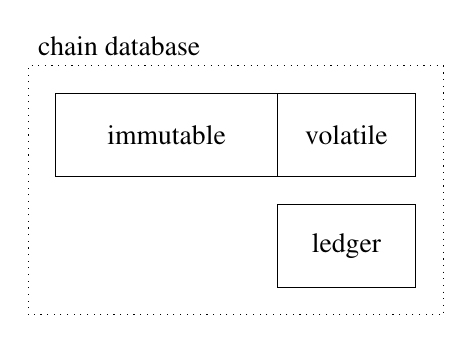
\begin{tikzpicture}
\draw [dotted]
     (-50pt, -65pt)
  -- ++(0, 90pt) node[above right] {chain database}
  -- ++(150pt, 0)
  -- ++(0, -90pt)
  -- cycle;
\node [draw, shape=rectangle, minimum width=80pt, minimum height=30pt] at (0,0)  {immutable};
\node [draw, shape=rectangle, minimum width=50pt, minimum height=30pt] at (65pt, 0)  {volatile};
\node [draw, shape=rectangle, minimum width=50pt, minimum height=30pt] at (65pt, - 40pt) {ledger};
\end{tikzpicture}

Discuss the immutable/volatile split (we reference this section for that).

\section{In memory}
\label{storage:inmemory}

TODO: After we discussed the overview, we should give an overview of everything
we store in memory in any component, so that we have a better understanding of
memory usage of the chain DB as a whole.

\subsection{Chain fragments}
\label{storage:fragments}

\subsection{Extended ledger state}
\label{storage:extledgerstate}
\label{storage:headerstate}

TODO: Is there a more natural place to talk about this? Introducing the
header state when introducing the storage layer does not feel quite right.
The storage layer might be storing the header state, but that doesn't
explain its existence.

ChainDepState, (ChainIndepState), LedgerState, ExtLedgerState

\chapter{Non-functional requirements}
\label{nonfunctional}

This whole chapter is Duncan-suitable :)
\duncan

\section{Network layer}
\label{nonfunctional:network}

This report is not intended as a comprehensive discussion of the network layer;
see \cite{network-spec} instead. However, in order to understand
some of the design decisions in the consensus layer we need to understand some
of the requirements imposed on it by the network layer.

TODOs:

\begin{itemize}
\item Highlight relevant aspects of the design of the network layer
\item Discuss requirements this imposes on the consensus layer
Primary example: Forecasting.
\item How do we keep the overlap between network and consensus as small
as possible? Network protocols do not involve consensus protocols
(chain sync client is not dependent on chain selection). Chain sync
client + "pre chain selection" + block download logic keeps things isolated.
\item Why do we even want to validate headers ahead of time? (Thread model etc.)
(Section for Duncan?).
Section with a sketch on an analysis of the amortised cost for attackers versus
our own costs to defend against it ("budget for work" that grows and shrinks
as you interact with a node).
\end{itemize}

\subsection{Header/Body Split (aka: Header submission)}
\label{nonfunctional:network:headerbody}

Discuss the chain fragments that we store per upstream node.
Discuss why we want to validate headers here -- without a full ledger state
(necessarily so, since no block bodies -- can't update ledger state): to prevent
DoS attacks.
(\cref{ledger:forecasting} contains a discussion of this from the point of view of
the ledger).
Forward reference to the chain sync client (\cref{chainsyncclient}).
Discuss why it's useful if the chain sync client can race ahead  for
\emph{performance} (why it's required for chain selection is the discussed in
\cref{forecast:ledgerview}).

See also section on avoiding the stability window
(\cref{low-density:pre-genesis}).

\subsection{Block submission}
\label{nonfunctional:network:blocksubmission}

Forward reference to \cref{servers:blockfetch}.

\subsection{Transaction submission}
\label{nonfunctional:network:txsubmission}

Mention that these are defined entirely network side, no consensus involvement
(just an abstraction over the mempool).

\section{Security "cost" concerns}

TODO: Look through the code and git history to find instances of where we
one way but not the other because it would give an attacker an easy way to
make it do lots of work (where were many such instances).

Fragile. Future work: how might be make this less brittle?
Or indeed, how might we test this?

Counter-examples (things we don't want to do)

\begin{itemize}
\item Parallel validation of an entire epoch of data (say, crypto only).
You might do a lot of work before realising that that work was not needed because
of an invalid block in the middle.
\end{itemize}

Future work: opportunities for parallelism that we don't yet exploit
(important example: script evaluation in Goguen).

\section{Hard time constraints}

Must produce a block on time, get it to the next slot leader

Bad counter-example: reward calculation in the Shelley ledger bad
(give examples of why).

\section{Predictable resource requirements}
\label{nonfunctional:best-is-worst}

make best == worst

(not \emph{just} a security concern: a concern even if every node honest)

\section{Resource registry}
\label{nonfunctional:resourceregistry}

In order to deal with resource allocation and deallocation, we use the
abstraction of the \lstinline!ResourceRegistry!. The resource registry is a
generalization of the \lstinline!bracket! pattern. Using a bracket imposes strict
rules on the scope of the allocated variables, as once the body of the
\lstinline!bracket! call finishes, the resources will be deallocated.

On some situations this is too constraining and resources, despite the need to
ensure they are deallocated, need to live for longer periods or be shared by
multiple consumers. The registry itself lives in a \lstinline!bracket!-like
environment, but the resources allocated in it can be opened and closed at any
point in the lifetime of the registry and will ultimately be closed when the
registry is being closed if they are still open at that time.

The allocation function for a given resource will run with exceptions
unconditionally masked, therefore in an uninterruptible fashion. Because of
this, it is important that such functions are fast. Note that once the
allocation call finishes, the resource is now managed by the registry and will
be deallocated in case an exception is thrown.

A resource that is allocated will be returned coupled with its
\lstinline!ResourceKey! that can be used to release the resource as it holds a
reference to the registry in which it is allocated.

Special care must be used when resources are dependent on one another. For
example, a thread allocated in the registry might hold some mutable reference to
a file handle that is replaced at certain points during the execution. In such
cases, the sequence of deallocation must take this into account and deallocate
the resources in reverse order of dependency.

Also when deallocating the resources, we must ensure that the right order of
deallocation is preserved. Right order here means that as resources that were
allocated later than others could potentially use the latter, the later ones
should probably be deallocated before the earlier ones (unless otherwise taken
care of). Resources in the registry are indexed by their \emph{age} which is a
meaningless backwards counter. A resource is considered older than another if
its age is greater than the one of the other resource. Conversely, a resource is
considered younger if the opposite holds.

\subsection{Temporary registries}
\label{nonfunctional:temporaryregs}

When some resources are not meant to be directly allocated in a registry, one
can take advantage of temporary resource registries as a temporary container for
those resources. For this purpose, the \lstinline!WithTempRegistry! is made
available. It is basically a \lstinline!StateT! computation which will check
that the resource was indeed transferred properly to the returned value and then
the registry will vanish.

Using this construction will ensure that if an exception is thrown while the
resources are being allocated but before they are kept track by the resulting
state, they will be released as the registry itself will close in presence of an
exception. Note that once the resource was transferred to the final state, no
more tracking is performed and the resource could be leaked. It is then
responsibility of the resulting state to eventually deallocate the resource, and
so that resulting state must itself ultimately be for example tracked by a
registry.

Temporary registries are useful when we want to run localized allocations and
checks, i.e. allocations and checks that use implementation details that should
remain hidden for upper layers. This is specially useful when we expect to run a
computation that will provide a result that holds some API which references some
internal data types which are not directly accessible from the API, but we still
want to run some checks on those internal data types. \footnote{See
  \lstinline!VolatileDB.openDB! for an example. The inner computation allocates
  and performs checks against a \lstinline!OpenState blk h! whereas the returned
  value is a \lstinline!VolatileDB! which has a \lstinline!close! function but
  otherwise has no direct access to the internal \lstinline!OpenState blk h!.}
The resulting value will be transitively closable from the general registry
through functions on the API (deallocating its resources), but the actual value
is not accessible to perform the checks usually involved with
\lstinline!WithTempRegistry!.

Note that if we just run the inner computation and return the API value, there
is a short time span during which an exception would leak the resources as the
API that can close the resources is not yet included in any exception handler
that will close it. A special case of this situation is when we run a
computation with a (\emph{upper}) registry and we want to perform a localized
allocation and checks on an internal component. The combinator
\lstinline!runInnerWithTempRegistry! is provided. This combinator will make sure
that the composite resource is allocated in the \emph{upper} registry before
closing the inner one (therefore performing the allocation checks against the
resulting inner state), and thus in presence of an exception the resources will
be safely deallocated. There are a couple of subtleties here that are worth
being mentioned:

\begin{itemize}
  \item There is a short time span during which the inner registry has not yet
        vanished, but the resource has already been allocated in the greater
        registry. An exception in this exact moment will lead to double freeing
        a resource.
  \item Unless the greater resulting state has some way of accessing the
        returned inner state, the function that performs the checks will
        necessarily be degenerate (i.e. \lstinline!const (const True)!). If we
        had a way to access the inner returned state, we could run the checks,
        but adding this implies leaking the inner state, its representation and
        functions, and most of the time this is not desirable as those are
        usually private implementation details.
\end{itemize}

\paragraph{Alternative: Specialization to \lstinline!TrackingTempRegistry!} The
\lstinline!TempRegistry! concept could be specialized in a narrower concept, a
\lstinline!TrackingTempRegistry! which would essentially be equivalent to a
\lstinline!TempRegistry () m! and no checks would be preformed on the resulting
state. This way some redundant situations could be simplified. Note that this is
also equivalent to using a special \lstinline!ResourceRegistry! which works as a
normal \lstinline!ResourceRegistry! but instead of deallocating them, it would
just untrack all the allocated resources when going out of scope.


\part{Consensus Layer}

\chapter{Consensus Protocol}
\label{consensus}

% TODO: what kind of variation does this design support?
% (counter-example: genesis rule)

% TODO: Describe API
%
% TODO: State invariants
%
% TODO: Discuss relationship to the Ouroboros papers. Where are the various parts
% of the paper implemented? How do additional design constraints change this?
% (e.g. header/body split)

\section{Overview}

\subsection{Chain selection}
\label{consensus:overview:chainsel}

Chain selection is the process of choosing between multiple competing chains,
and is one of the most important responsibilities of a consensus protocol. When
choosing between two chains, in theory any part of those chains could be
relevant; indeed, the research literature typically describes chain selection as
a comparison of two entire chains (\cref{bft-paper,praos-paper}). In practice
that is not realistic: the node has to do chain selection frequently, and
scanning millions of blocks each time to make the comparison is of course out of
the question.

The consensus layer keeps the most recent headers as a \emph{chain fragment}
in memory (\cref{storage:inmemory}); the rest of the chain is stored on disk.
Similarly, we keep a chain fragment of headers in memory for every (upstream)
node whose chain we are following and whose blocks we may wish to adopt
(\cref{chainsyncclient}). Before the introduction of the hard fork combinator
chain selection used to be given these fragments to compare; as we will discuss
in \cref{hfc:intro}, however, this does not scale so well to hybrid chains.

It turns out, however, that it suffices to look only at the headers at the very
tip of the chain, at least for the class of consensus algorithms we need to
support. The exact information we need about that tip varies from
one protocol to the other, but at least for the Ouroboros family of consensus
protocols the essence is always the same: we prefer longer chains over shorter
ones (justifying \emph{why} this is the right choice is the domain  of
cryptographic research and well outside the scope of this report). In the
simplest case, the length of the chain is \emph{all} that matters, and hence the
only thing we need to know about the blocks at the tips of the chains is their
block numbers.\footnote{It doesn't actually matter if the actual block headers
contain a block number or not; if they don't, we can add a ``virtual field''
to the in-memory representation of the block header. For block headers that
\emph{do} include a block number (which is the case for the Cardano chain),
header  validation verifies that the block number is increasing. Note that EBBs
complicate this particular somewhat; see page~\pageref{ebb-chain-selection}.}

This does beg the question of how to compare two chains when one (or both) of
them are empty, since now we have no header to compare. We will resolve this by
stating the following fundamental assumption about \emph{all} chain selection
algorithms supported by the consensus layer:

\begin{assumption}[Prefer extension]
\label{prefer-extension}
The extension of a chain is always preferred over that chain.
\end{assumption}

A direct consequence of \cref{prefer-extension} is that a non-empty chain is
always preferred over an empty one,\footnote{Comparing empty chain
\emph{fragments}, introduced in \cref{storage:fragments}, is significantly more
subtle, and will be discussed in \cref{chainsel:fragments}.} but we will
actually need something stronger than that: we insist that shorter chains can
never be preferred over longer ones:

\begin{assumption}[Never Shrink]
\label{never-shrink}
A shorter chain is never preferred over a longer chain.
\end{assumption}

\Cref{never-shrink} does not say anything about chains of equal length; this will
be important for Praos (\cref{praos}). An important side-note here is that
the Ouroboros Genesis consensus protocol includes a chain selection rule
(the genesis rule) that violates \cref{never-shrink} (though not \cref{prefer-extension}); it also cannot be defined by only looking at the tips of chains.
It will therefore require special treatment; we will come back to this in
\cref{genesis}.

\subsection{The security parameter $k$}
\label{consensus:overview:k}

When the Cardano blockchain was first launched, it was using a consensus
protocol that we now refer to as Ouroboros Classic \cite{cryptoeprint:2016:889}.
The re-implementation of the consensus layer never had support for Ouroboros
Classic, instead using Ouroboros BFT \cite{cryptoeprint:2018:1049} as a
transitional protocol towards Ouroboros Praos \cite{cryptoeprint:2017:573},
which is the consensus protocol in use at the time of writing, with plans to
switch to Ouroboros Genesis \cite{cryptoeprint:2018:378} relatively soon
(\cref{genesis}).

Both Ouroboros Classic and Ouroboros Praos are based on a chain selection rule
that imposes a maximum rollback condition: alternative chains to a node's
current chain that fork off more than a certain number of blocks ago are never
considered for adoption. This limit is known as the \emph{security parameter},
and is usually denoted by $k$; at present $k = 2160$ blocks. The Ouroboros
analysis shows that consensus will be reached despite this maximum rollback
limitation; indeed, this maximum rollback is \emph{required} in order to reach
consensus (we discuss this in some detail in
\cref{genesis:background:longest-chain}).

For Ouroboros BFT and Ouroboros Genesis the situation is slightly different:

\begin{itemize}
\item Ouroboros BFT does not impose a maximum rollback, but adding such a
requirement does not change the protocol in any fundamental way: the analysis
for Ouroboros Praos shows that nodes will not diverge more than $k$ blocks, and
since BFT converges much quicker than that, adding this (large) maximum rollback
requirement does not change anything.
\item The analysis that shows that nodes will not diverge by more than $k$
blocks does of course not apply to new nodes joining the system. Indeed, when
using Ouroboros Praos, such nodes are vulnerable to an attack where an adversary
with some stake (does not have to be much) presents the newly joining node with
a chain that diverges by more than $k$ blocks from the honest chain, at which
point point the node would become unable to switch to the real chain. Solving
this is the purview of Ouroboros Genesis.

Like Ouroboros BFT, Ouroboros Genesis likewise does not impose a maximum
rollback, \emph{but} the analysis \cite{cryptoeprint:2018:378} shows that when
nodes are up to date, they can employ the Ouroboros Praos rule (i.e., the rule
\emph{with} the maximum rollback requirement). This is not true when the node is
behind and is catching up, but the main goal of \cref{genesis} is to show how we
can nonetheless avoid rollbacks exceeding $k$ blocks even when a node is
catching up.
\end{itemize}

Within the consensus layer we therefore assume that we \emph{always} have a
limit $k$ on the number of blocks we might have to rollback. We take advantage
of this in many ways; here we just mention a few:

\begin{itemize}
\item We use it as an organising principle in the storage layer
(\cref{storage}), dividing the chain into a part that we know is stable (the
"immutable chain"), and a part near the tip that is still subject to rollback
(the "volatile chain"). Block lookup into the immutable chain is very efficient,
and since the vast majority of the chain is immutable, this helps improve
overall efficiency of the system.

\item When we switch to a new fork by rolling back and then adopting some new
blocks, those new blocks must be verified against the ledger state as it was
at the point we rolled back to. This means we must be able to construct
historical ledger states. In principle this is always possible, as we can always
replay the entire chain, but doing so would be expensive. However, since we have
a limit on the maximum rollback, we also have a limit on how old the oldest
ledger state is we might have to reconstruct; we take advantage of this in the
Ledger Database (\cref{ledgerdb}) which can efficiently reconstruct any of those
$k$ historical ledger states.

\item We need to keep track of the chains of our peer nodes in order to be able
to decide whether or not we might wish to switch to those chains
(\cref{chainsyncclient}). For consensus protocols based on a longest chain rule
(such as Ouroboros Praos), this means that we would need to download and verify
enough blocks from those alternative chains that the alternative chain becomes
longer than our own. Without a maximum rollback, this would be an unbounded
amount of work as well as an unbounded amount of data we would have to store.
A maximum rollback of $k$, however, means that validating (and storing) $k+1$
blocks should be sufficient.\footnote{For chain selection algorithms such as
Ouroboros Genesis which are based on properties of the chains near their
\emph{intersection point} rather than near their tips this is less relevant.}
\end{itemize}

Of course, a maximum rollback may be problematic in the case of severe network
outages that partition the nodes for extended periods of time (in the order of
days). When this happens, the chains will diverge and recovering converge will
need manual intervention; this is true for any of the consensus protocols
mentioned above. This manual intervention is outside the scope of this report.

\section{The \lstinline!ConsensusProtocol! Class}
\label{consensus:class}

We model consensus protocols as a single class called
\lstinline!ConsensusProtocol!; this class can be considered to be the
central class within the consensus layer.

\begin{lstlisting}
class (..) => ConsensusProtocol p where
\end{lstlisting}

The type variable $p$ is a type-level tag describing a particular consensus
protocol; if Haskell had open kinds\footnote{We will come back to this in
\cref{future:openkinds}.}, we could say \lstinline!(p :: ConsensusProtocol)!.
All functions within this class take an argument of type
%
\begin{lstlisting}
data family ConsensusConfig p :: Type
\end{lstlisting}
%
This allows the protocol to depend on some static configuration data; what
configuration data is required will vary from protocol to
protocol.\footnote{Explicitly modelling such a required context could be avoided
if we used explicit records instead of type classes; we will discuss this point
in more detail in \cref{technical:classes-vs-records}.}  The rest of the
consensus layer does not really do much with this configuration, except make it
available where required; however, we do require that whatever the configuration
is, we can extract $k$ from it:
%
\begin{lstlisting}
protocolSecurityParam :: ConsensusConfig p -> SecurityParam
\end{lstlisting}
%
For example, this is used by the chain database to determine when blocks can be
moved from the volatile DB to the immutable DB (\cref{storage:components}). In
the rest of this section we will consider the various parts of the
\lstinline!ConsensusProtocol! class one by one.

\subsection{Chain selection}
\label{consensus:class:chainsel}

As mentioned in \cref{consensus:overview:chainsel}, chain selection will only
look at the headers at the tip of the ledger. Since we are defining consensus
protocols independent from a concrete choice of ledger, however
(\cref{decouple-consensus-ledger}), we cannot use a concrete block or header
type. Instead, we merely say that the chain selection requires \emph{some} view
on headers that it needs to make its decisions:

\begin{lstlisting}
type family SelectView p :: Type
type SelectView p = BlockNo
\end{lstlisting}

The default is \lstinline!BlockNo! because as we have seen this is all that is
required for the most important chain selection rule, simply preferring longer
chains over shorter ones. It is the responsibility of the glue code that
connects a specific choice of ledger to a consensus protocol to define the
projection from a concrete block type to this \lstinline!SelectView!
(\ref{BlockSupportsProtocol}). We then require that these views must be
comparable
%
\begin{lstlisting}
class (Ord (SelectView p), ..) => ConsensusProtocol p where
\end{lstlisting}
%
and say that one chain is (strictly) preferred over another if its
\lstinline!SelectView! is greater. If two chains terminate in headers with
the \emph{same} view, neither chain is preferred over the other, and we
could pick either one (we say they are equally preferable).

Later in this chapter we will discuss in detail how our treatment of
consensus algorithms differs from the research literature (\cref{bft,praos}),
and in \cref{chainsel} we will see how the details of how chain selection
is implemented in the chain database; it is worth pointing out here, however, that the comparison based on \lstinline!SelectView! is not intended to capture

\begin{itemize}
\item chain validity
\item the intersection point (checking that the intersection point is not too
far back, preserving the invariant that we never roll back more than $k$ blocks,
see \cref{consensus:overview:k})
\end{itemize}

Both of these responsibilities would require more than seeing just
the tip of the chains. They are handled independent of the choice of
consensus protocol by the chain database, as discussed in \cref{chainsel}.

When two \emph{candidate} chains (that is, two chains that aren't our current)
are equally preferable, we are free to choose either one. However, when a
candidate chain is equally preferable to our current, we \emph{must} stick
with our current chain. This is true for all Ouroboros consensus protocols,
and we define it once and for all:

\begin{lstlisting}
preferCandidate ::
     ConsensusProtocol p
  => proxy      p
  -> SelectView p  -- ^ Tip of our chain
  -> SelectView p  -- ^ Tip of the candidate
  -> Bool
preferCandidate _ ours cand = cand > ours
\end{lstlisting}

\subsection{Ledger view}
\label{consensus:class:ledgerview}

We mentioned in \cref{overview:ledger} that some consensus protocols may require
limited information from the ledger; for instance, the Praos consensus protocol
needs access to the stake distribution for the leadership check. In the
\lstinline!ConsensusProtocol! abstraction, this is modelled as a \emph{view}
on the ledger state

\begin{lstlisting}
type family LedgerView p :: Type
\end{lstlisting}

The ledger view will be required in only one function: when we ``tick'' the
state of the consensus protocol. We will discuss this state management in more
detail next.

\subsection{Protocol state management}
\label{consensus:class:state}

Each consensus protocol has its own type chain dependent state\footnote{We are
referring to this as the ``chain dependent state'' to emphasise that this is
state that evolves with the chain, and indeed is subject to rollback when we
switch to alternatives forks. This distinguishes it from chain
\emph{independent} state such as evolving private keys, which are updated
independently from blocks and are not subject to rollback.}

\begin{lstlisting}
type family ChainDepState p :: Type
\end{lstlisting}

The state must be updated with each block that comes in, but just like for
chain selection, we don't work with a concrete block type but instead define a
\emph{view} on blocks that is used to update the consensus state:

\begin{lstlisting}
type family ValidateView p :: Type
\end{lstlisting}

We're referring to this as the \lstinline!ValidateView! because updating the
consensus state also serves as \emph{validation} of (that part of) the block;
consequently, validation can also \emph{fail}, with protocol specific error
messages:

\begin{lstlisting}
type family ValidationErr p :: Type
\end{lstlisting}

Updating the chain dependent state now comes as a pair of functions. As for the ledger
(\cref{overview:ledger}), we first \emph{tick} the protocol state to the
appropriate slot, passing the already ticked ledger view as an
argument:\footnote{Throughout the consensus layer, the result of ticking is
distinguished from the unticked value at the type level. This allows to store
additional (or indeed, less) information in the ticked ledger state, but also
clarifies ordering. For example, it is clear in \lstinline!tickChainDepState!
that the ledger view we pass as an argument is already ticked, as opposed to the
\emph{old} ledger view.}

\begin{lstlisting}
tickChainDepState ::
     ConsensusConfig p
  -> Ticked (LedgerView p)
  -> SlotNo
  -> ChainDepState p
  -> Ticked (ChainDepState p)
\end{lstlisting}

As an example, the Praos consensus protocol (\cref{praos}) derives its
randomness from the  chain itself. It does that by maintaining a set of random
numbers called \emph{nonces}, which are used as seeds to pseudo-random number
generators. Every so often the current nonce is swapped out for a new one; this
does not depend on the specific block, but merely on a certain slot number being
reached, and hence is an example of something that the ticking function should
do.

The (validation view on) a block can then be applied to the already ticked
protocol state:

\begin{lstlisting}
updateChainDepState ::
     ConsensusConfig       p
  -> ValidateView          p
  -> SlotNo
  -> Ticked (ChainDepState p)
  -> Except (ValidationErr p) (ChainDepState p)
\end{lstlisting}

Finally, there is a variant of this function that can we used to \emph{reapply}
a known-to-be-valid block, potentially skipping expensive cryptographic checks,
merely computing what the new state is:

\begin{lstlisting}
reupdateChainDepState ::
     ConsensusConfig       p
  -> ValidateView          p
  -> SlotNo
  -> Ticked (ChainDepState p)
  -> ChainDepState         p
\end{lstlisting}

Re-applying previously-validated blocks happens when we are replaying blocks
from the immutable database when initialising the in-memory ledger state
(\cref{ledgerdb:on-disk:initialisation}). It is also useful during chain
selection (\cref{chainsel}): depending on the consensus protocol, we may end up
switching relatively frequently between short-lived forks; when this happens,
skipping expensive checks can improve the performance of the node. \todo{How
  does this relate to the best case == worst case thing? Or to the asymptotic
  attacker/defender costs?}

\subsection{Leader selection}
\label{consensus:class:leaderselection}

The final responsibility of the consensus protocol is leader selection. First,
it is entirely possible for nodes to track the blockchain without ever producing
any blocks themselves; indeed, this will be the case for the majority of
nodes\footnote{Most ``normal'' users will not produce blocks themselves, but
instead delegate their stake to stakepools who produce blocks on their behalf.}
In order for a node to be able to lead at all, it may need access to keys and
other configuration data; the exact nature of what is required is different
from protocol to protocol, and so we model this as a type family

\begin{lstlisting}
type family CanBeLeader p :: Type
\end{lstlisting}

A value of \lstinline!CanBeLeader! merely indicates that the node has the
required configuration to lead at all. It does \emph{not} necessarily mean that
the node has the right to lead in any particular slot; \emph{this} is indicated
by a value of type \lstinline!IsLeader!:

\begin{lstlisting}
type family IsLeader p :: Type
\end{lstlisting}

In simple cases \lstinline!IsLeader! can just be a unit value (``yes, you are a
leader now'') but for more sophisticated consensus protocols such as Praos this
will be a cryptographic proof that the node indeed has the right to lead in this
slot. Checking whether a that \emph{can} lead \emph{should} lead in a given slot
is the responsibility of the final function in this class:

\begin{lstlisting}
checkIsLeader ::
     ConsensusConfig       p
  -> CanBeLeader           p
  -> SlotNo
  -> Ticked (ChainDepState p)
  -> Maybe (IsLeader       p)
\end{lstlisting}

\section{Connecting a block to a protocol}
\label{BlockSupportsProtocol}

Although a single consensus protocol might be used with many blocks, any given
block is designed for a \emph{single} consensus protocol. The following type
family witnesses this relation:\footnote{For a discussion about why we
choose to make some type families top-level definitions rather than associate
them with a type class, see \cref{technical:toplevel-vs-associated}.}
%
\begin{lstlisting}
type family BlockProtocol blk :: Type
\end{lstlisting}
%
Of course, for the block to be usable with that consensus protocol, we need
functions that construct the \lstinline!SelectView!
(\cref{consensus:class:chainsel}) and \lstinline!ValidateView!
(\cref{consensus:class:state}) projections from that block:
%
\begin{lstlisting}
class (..) => BlockSupportsProtocol blk where
  validateView ::
       BlockConfig blk
    -> Header blk -> ValidateView (BlockProtocol blk)

  selectView ::
       BlockConfig blk
    -> Header blk -> SelectView (BlockProtocol blk)
\end{lstlisting}
%%
The \lstinline!BlockConfig! is the static configuration required to work with
blocks of this type; it's just another data family:
%
\begin{lstlisting}
data family BlockConfig blk :: Type
\end{lstlisting}

\section{Design decisions constraining the Ouroboros protocol family}
\label{design-decisions-constraining-ouroboros}

\todo{TODO} TODO: Perhaps we should move this to conclusions; some of these
requirements may only become clear in later chapters (like the forecasting
range).

\todo{TODO} TODO: The purpose of this section should be to highlight design
decisions we're already covering in this chapter that impose constraints
on existing or future members of the Ouroboros protocol family.

For example, we at least have:
\begin{itemize}
\item max-K rollback, we insist that there be a maximum rollback length. This
was true for Ouroboros Classic, but is not true for Praos/Genesis, nevertheless
we insist on this for our design. We should say why this is so helpful for our
design. We should also admit that this is a fundamental decision on liveness vs
consistency, and that we're picking consistency over liveness. The Ouroboros
family is more liberal and different members of that family can and do make
different choices, so some adaptation of protocols in papers may be needed to
fit this design decision. In particular this is the case for Genesis. We cannot
implement Genesis as described since it is not compatible with a rollback limit.

\item We insist that we can compare chains based only on their tips. For example
even length is a property of the whole chain not a block, but we insist that
chains include their length into the blocks in a verifiable way, which enables
this tip-only checking. Future Ouroboros family members may need some adaptation
to fit into this constraint. In particular the Genesis rule as described really
is a whole chain thing. Some creativity is needed to fit Genesis into our
framework: e.g. perhaps seeing it not as a chain selection rule at all but as a
different (coordinated) mode for following headers.

\item We insist that a strict extension of a chain is always preferred over
that chain.

\item We insist that we never roll back to a strictly shorter chain.

\item The minimum cyclic data dependency time: the minimum time we permit
between some data going onto the chain and it affecting the validity of blocks
or the choices made by chain selection. This one is a constraint on both the
consensus algorithm and the ledger rules. For example this constrains the Praos
epoch structure, but also ledger rules like the Shelley rule on when genesis
key delegations or VRF key updates take effect. We should cover why we have this
constraint: arising from wanting to do header validation sufficiently in advance
of block download and validation that we can see that there's a potential longer
valid chain.

\item The ledger must be able to look ahead sufficiently to validate $k + 1$
headers (to guarantee a roll back of $k$). \todo{TODO}TODO: We should discuss
this in more detail.
\end{itemize}

\section{Permissive BFT}
\label{bft}

Defined in \cite{byron-chain-spec}
Not to be confused with ``Practical BFT'' \cite{10.1145/571637.571640}

\subsection{Background}
\label{bft:background}

\duncan
Discuss \emph{why} we started with Permissive BFT (backwards compatible with
Ouroboros Classic).

\subsection{Implementation}

\subsection{Relation to the paper}
\label{bft-paper}

Permissive BFT is a variation on Ouroboros BFT, defined in
\cite{cryptoeprint:2018:1049}. We have included the main protocol description
from that paper as \cref{figure:bft} in this document; the only difference is
that we've added a few additional labels so we can refer to specific parts of
the protocol description below.

It will be immediately obvious from \cref{figure:bft} that this description
covers significantly more than what we consider to be part of the consensus
protocol proper here. We will discuss the various parts of the BFT protocol
description below.

\begin{description}
  \item[Clock update and network delivery] The BFT specification requires that
  ``with each advance of the clock (..) a collection of transactions and
  blockchains are pushed to the server''. We consider neither block submission
  nor transaction submission to be within the scope of the consensus algorithm;
  see \cref{nonfunctional:network:blocksubmission,servers:blockfetch} and
  \cref{nonfunctional:network:blocksubmission,servers:txsubmission} instead, respectively.

  \item[Mempool update] (\cref{bft:mempool}). The design of the mempool is the
  subject of \cref{mempool}. Here we only briefly comment on how it relates to
  what the BFT specification assumes:
%
  \begin{itemize}
    \item \textit{Consistency} (\cref{bft:mempool:consistency}). Our mempool
    does indeed ensure consistency. In fact, we require something strictly
    stronger; see \cref{mempool:consistency} for details.
    \item \textit{Time-to-live (TTL)} (\cref{bft:mempool:ttl}). The BFT
    specification requires that transactions stay in the mempool for a maximum
    of $u$ rounds, for some configurable $u$. Our current mempool does not have
    explicit support for a TTL parameter. The Shelley ledger will have support
    for TTL starting with the ``Allegra'' era, so that transactions are only
    valid within a certain slot window; this is part of the normal ledger rules
    however and requires no explicit support from the consensus layer. That's
    not to say that explicit support would not be useful; see \cref{future:ttl}
    in the chapter on future work.
    \item \textit{Receipts} (\cref{bft:mempool:receipts}). We do not offer any
    kind of receipts for inclusion in the mempool. Clients such as wallets must
    monitor the chain instead (see also \cite{wallet-spec}). The BFT
    specification marks this as optional so this is not a deviation.
  \end{itemize}
%
  \item[Blockchain update] (\cref{bft:update}). The BFT specification requires
  that the node prefers any valid chain over its own, as long as its strictly
  longer. \emph{We do not satisfy this requirement.} The chain selection rule
  for Permissive BFT is indeed the longest chain rule, \emph{but} consensus
  imposes a global maximum rollback (the security parameter $k$;
  \cref{consensus:overview:k}). In other words, nodes \emph{will} prefer longer
  chains over its own, \emph{provided} that the intersection between that chain
  and the nodes own chain is no more than $k$ blocks away from the node's tip.
  \todo{Justify this maximum rollback?}

  Moreover, our definition of validity is also different. We do require that
  hashes line up (\cref{bft:update:hash}), although we do not consider this part
  of the responsibility of the consensus protocol, but instead require this
  independent of the choice of consensus protocol when updating the header state
  (\cref{storage:headerstate}). We do of course also require that the transactions in
  the block are valid (\cref{bft:update:body}), but this is the responsibility
  of the ledger layer instead (\cref{ledger}); the consensus protocol should be
  independent from what's stored in the block body.

  Permissive BFT is however different from BFT \emph{by design} in the
  signatures we require.\footnote{\label{footnote:singlesignature}There is
  another minor deviation from the specification: we don't require an explicit
  signature on the block body. Instead, we have a single signature over the
  header, and the header includes a \emph{hash} of the body.} BFT requires that
  each block is signed strictly according to the round robin schedule
  (\cref{bft:update:signatures}); the whole point of \emph{permissive} BFT is
  that we relax this requirement and merely require that blocks are signed by
  \emph{any} of the known core nodes.

  Permissive BFT is however not \emph{strictly} more permissive than BFT:
  although blocks do not need to be signed according to the round robin
  schedule, there is a limit on the number of signatures by any given node in a
  given window of blocks. When a node exceeds that threshold, its block is
  rejected as invalid. Currently that threshold is set to 0.22 \cite[Appendix A,
  Calculating the $t$ parameter]{byron-chain-spec}, which was considered to be
  the smallest value that would be sufficiently unlikely to consider a chain
  generated by Ouroboros Classic as invalid (\cref{bft:background}) and yet give
  as little leeway to a malicious node as possible. This has an unfortunate side
  effect, however. BFT can always recover from network partitions \cite[Section
  1, Introduction]{cryptoeprint:2018:1049}, but this is not true for PBFT: in a
  setting with 7 core nodes (the same setting as considered in the PBFT
  specification), a 4:3 network partition would quickly lead to \emph{both}
  partitions being unable to produce more blocks; after all, the nodes in the
  partition of 4 nodes would each sign 1/4th of the blocks, and the nodes in the
  partition of 3 nodes would each sign 1/3rd. Both partitions would therefore
  quickly stop producing blocks. Picking 0.25 for the threshold instead of 0.22
  would alleviate this problem, and would still be conform the PBFT
  specification, which says that the value must be in the closed interval
  $[\frac{1}{5}, \frac{1}{4}]$. Since PBFT is however no longer required (the
  Byron era is past and fresh deployments would not need Permissive BFT but
  could use regular BFT), it's probably not worth reconsidering this, although
  it \emph{is} relevant for the consensus tests (\cref{testing:dire}).
%
  \item[Blockchain extension] (\cref{bft:extension}).
  The leadership check implemented as part of PBFT is conform specification
  (\cref{bft:leadershipcheck}). The rest of this section matches the
  implementation, modulo some details some of which we already alluded to above:
%
  \begin{itemize}
    \item The block format is slightly different; for instance, we only have a
    single signature (\cref{footnote:singlesignature}).
    \item Blocks in Byron have a maximum size, so we cannot necessarily take
    \emph{all} valid transactions from the mempool.
    \item Block diffusion is not limited to the suffix of the chain: clients
    can request \emph{any} block that's on the chain. This is of course critical
    to allow nodes to join the network later, something which the BFT paper does
    not consider.
  \end{itemize}
%
  It should also be pointed out that we consider neither block production nor
  block diffusion to be part of the consensus protocol at all; only the
  leadership check itself is.

  \item[Ledger reporting].
  Although we do offer a way to query the state of the ledger
  (\cref{ledger:queries}), we do not offer a query to distinguish between
  finalised/pending blocks.
  \todo{TODO} TODO: It's also not clear to me why the BFT specification would
  consider a block to be finalised as soon as it's $3t + 1$ blocks deep
  (where $t$ is the maximum number of core nodes). The paper claims that BFT
  can always recover from a network partition, and the chain selection rule
  in the paper requires supporting infinite rollback.

\end{description}

\begin{figure}
\small
\hrule
\textbf{Parameters}:

\vspace{1em}

\begin{tabular}{c|l}
$n$ & total number of core nodes \\
$t$ & maximum number of core nodes \\
    & (we do not make this distinction between $n$ and $t$ in the consensus layer, effectively setting $n = t$) \\
$u$ & time to live (TTL) of a transaction \\
\end{tabular}

\vspace{1em}

\textbf{Protocol}: \\

The $i$-th server locally maintains a blockchain $B_0 B_1 \ldots B_l$, an
ordered sequence of transactions called a mempool, and carries out the following
protocol:

\begin{description}
  \item[Clock update and network delivery] With each advance of the clock to a
  slot $\mathit{sl}_j$, a collection of transactions and blockchains are pushed
  to the server by the network layer. Following this, the server proceeds as
  follows:
  %
  \begin{enumerate}
    \item \textbf{Mempool update}.\label{bft:mempool}
      \begin{enumerate}
        \item \label{bft:mempool:consistency} Whenever a transaction
        $\mathit{tx}$ is received, it is added to the mempool as long as it is
        consistent with
        \begin{enumerate}
          \item the existing transactions in the mempool and
          \item the contents of the local blockchain.
        \end{enumerate}
        \item \label{bft:mempool:ttl} The transaction is maintained in the
        mempool for $u$ rounds, where $u$ is a parameter.
        \item \label{bft:mempool:receipts} Optionally, when the transaction
        enters the mempool the server can return a signed receipt back to the
        client that is identified as the sender.
      \end{enumerate}
%
  \item \textbf{Blockchain update}.\label{bft:update} Whenever the server
  becomes aware of an alternative blockchain
  $B_0 B_1' \ldots B'_s$
  with $s > l$, it replaces its local chain with this new chain provided it is
  valid, i.e. each one of its blocks
  $(h, d, \mathit{sl}_j, \sigma_\mathit{sl}, \sigma_\mathrm{block})$
%
  \begin{enumerate}
    \item \label{bft:update:signatures} contains proper signatures
    \begin{enumerate}
      \item one for time slot $\mathit{sl}_j$ and
      \item one for the entire block
    \end{enumerate}
    by server $i$ such that $i - 1 = (j - 1) \bmod n$
    \item \label{bft:update:hash} $h$ is the hash of the previous block, and
    \item \label{bft:update:body} $d$ is a valid sequence of transactions w.r.t.
    the ledger defined by the transactions found in the previous blocks
  \end{enumerate}
%
  \item \textbf{Blockchain extension}.\label{bft:extension} Finally, the server
  checks if it is responsible to issue the next block by testing if
%
  \begin{equation}
    i - 1 = (j - 1) \bmod n
  \label{bft:leadershipcheck}
  \end{equation}
%
  In such case, this $i$-th server is the slot leader. It
%
  \begin{itemize}
    \item collects the set $d$ of all valid transactions from its mempool and
    \item appends the block $B_{l+1} = (h, d, \mathit{sl}_j, \sigma_\mathit{sl}, \sigma_\mathrm{block})$ to its blockchain, where
    \begin{equation*}
      \begin{split}
      \sigma_\mathit{sl}    & = \mathsf{Sign}_{\mathsf{sk}_i}(\mathit{sl}_j) \\
      \sigma_\mathrm{block} & = \mathsf{Sign}_{\mathsf{sk}_i}(h, d, \mathit{sl}_j, \sigma_\mathit{sl}) \\
      h                     & = H(B_l) \\
      \end{split}
    \end{equation*}
    It then diffuses $B_{l+1}$ as well as any requested blocks from the suffix of its blockchain that covers the most recent $2t + 1$ slots.
    \end{itemize}

  \end{enumerate}

  \item[Ledger Reporting] Whenever queried, the server reports as ``finalised'' the ledger of transactions contained in the blocks $B_0 \ldots B_m, m \le l$, where $B_m$ has a slot time stamp more than $3t + 1$ slots in the past. Blocks $B_{m+1} \ldots B_l$ are reported as ``pending''.
\end{description}

\hrule
\caption{\label{figure:bft}Ouroboros-BFT \cite[Figure 1]{cryptoeprint:2018:1049}}
\end{figure}

\section{Praos}
\label{praos}

TODO: Discuss $\Delta$: When relating the papers to the implementation, we
loosely think of $\Delta$ as roughly having value 5, i.e., there is a maximum
message delay of 5 slots. However, this link to the paper is tenuous at best:
the messages the paper expects the system to send, and the messages that the
system \emph{actually} sends, are not at all the same. Defining how these relate
more precisely would be critical for a more formal statement of equivalence
between the paper and the implementation, but such a study is well outside the
scope of this report.

\subsection{Active slot coefficient}
\label{praos:f}

\subsection{Implementation}

\subsection{Relation to the paper}
\label{praos-paper}

\cite{cryptoeprint:2018:378}

\section{Combinator: Override the leader schedule}
\label{consensus:override-leader-schedule}

\cleardoublepage
\section{Separation of responsibility between consensus and ledger}

\subsection{Vision}

In the vision that underlies the abstract design of the consensus layer,
the separation of responsibility between the consensus layer and the
ledger layer happens along three axes.

\begin{description}
\item{Block \emph{selection} versus block \emph{contents}}

The primary objective of the consensus layer is to ensure that \emph{consensus}
is reached: that is, everyone agrees on (a sufficiently long prefix of) the
chain. From a sufficiently high vantage point, the consensus layer could
reasonably be described as an implementation of the various Ouroboros papers
(Praos, Genesis, etc.). A critical component of this is \emph{chain selection},
choosing between competing chains. The consensus layer does not need to be aware
of what is inside the blocks that it is choosing between.

By contrast, the ledger layer is not aware of multiple chains at all, and will
never need to execute chain selection: it exclusively deals with linear
histories. \emph{Its} primary objective is to define the contents of blocks,
along with rules that interpret those contents, computing the \emph{ledger
state}.

\item{\emph{Construction} versus \emph{verification}}

The ledger layer only ever deals with fully formed blocks. Its responsibility is
to \emph{verify} those blocks and describe how they transform the ledger state.
But those blocks need to come from somewhere in the first place; block
\emph{construction} is the responsibility of the consensus layer. This dichotomy
manifests itself in two ways:

\begin{itemize}
\item When the ledger layer verifies a block, it must verify whether or not the
node that produced the block had the right to do so, that is, whether or not it
was a slot leader in the block's slot (though it may be argued that this should
be a consensus concern instead, see below). Typically, it will need only access
to the node's \emph{public} key to do so. Note that multiple nodes may have the
right to produce a block in any given slot; the ledger layer is not checking
for \emph{the} slot leader, but rather for \emph{a} slot leader.

By contrast, the consensus layer is not checking if \emph{some} node is a leader
for slot, but rather whether \emph{it} is a leader for the current slot, and if
so, produce a block for that slot (along with evidence that it had the right to
do so). Typically, it will need access to the node's \emph{private} key in order
to execute that check.

\item Blocks are only valid with respect to a particular ledger state. Since
blocks specify their predecessor (the predecessor hash), they also implicitly
specify which ledger state they should be evaluated against: the ledger state
that was the result of applying that predecessor block (or the genesis ledger
state for the very first block).

By contrast, when the consensus layer produces a block, it must construct a
block that is valid with respect to the node's \emph{current} ledger state, and
\emph{choose} the predecessor of that new block to be the tip of the node's
current chain.

\end{itemize}

\item{\emph{Stateful} versus \emph{stateless}}

The ledger layer is entirely stateless: it is a pure function that accepts a
ledger state and a block as input and produces the new ledger state (or an
error if the block was invalid). State management is the responsibility of
the consensus layer:

\begin{itemize}

\item The consensus layer must maintain the current ledger state, and pass that
to the ledger layer when validating blocks that fit neatly onto the node's
current tip. In addition, the consensus must provide efficient access to
\emph{historical} ledger states, so that it can validate (and possibly adopt)
alternative forks of the chain.

\item Although the consensus layer does not need to be aware of the exact nature
of the block contents, it \emph{does} have to collect these ``transactions'' and
consider them when producing a block (the mempool, \cref{mempool}). If it
chooses to do eager transaction validation (that is, before it actually produces
a block), it will need support from the ledger layer to do; when producing a
block, it will need assistance from the ledger layer to produce the block body.

In both cases (transaction validation and block body construction), the
consensus layer is responsible for passing an appropriate ledger state to the
ledger layer. In the case of block production, the choice of ledger state is
clear: the current ledger state. For the mempool, it is slightly less clear-cut;
the mempool is effectively constructing a ``virtual'' block with a predecessor
chosen from the node's current chain, near its tip.\footnote{We could update
this ``virtual'' block every time that the node's current chain changes, so that
the virtual block's predecessor is always the current chain's tip. This however
couples two concurrent processes more tightly than required, and is moreover
costly: re-evaluating the mempool can be expensive.}

\end{itemize}

\end{description}

Ideally, the implementation of a particular consensus protocol (say, Praos)
should be usable with any choice of ledger (cryptocurrency or otherwise), and
conversely, a particular ledger (say, Shelley) should be usable with any choice
of consensus protocol  (Praos, Genesis, or indeed a different consensus protocol
entirely). The consensus protocol \emph{does} need some limited information from
the ledger, but we can provide this separately
(\cref{ledger:api:LedgerSupportsProtocol}), and abstract over what a particular
consensus algorithm needs from the ledger layer it is used with (specifically,
the \lstinline!SelectView! and the \lstinline!LedgerView!, discussed in
\cref{consensus:class:chainsel,consensus:class:ledgerview}).

\subsection{Practice}

In practice, the separation is not quite so clean. Partly this is for
historical reasons. When the Cardano blockchain was re-implemented, the new
consensus layer and the new ledger layer were developed in tandem, and it was
not always practical to have one wait for design decisions by the other.
For example, most of Praos is currently implemented in the ledger layer,
despite the ledger layer never having to do chain selection, ever. These are
issues that we can resolve with some relatively minor refactoring.

More problematic is that the current ledgers are not designed to be parametric
in a choice of consensus algorithm. Specifically, the Shelley ledger hardcodes
Praos. At some level, that statement makes no sense: the ledger layer never
needs to execute chain selection nor decide if it's a leader for a given slot.
However, the \emph{verification} of a block by the ledger layer currently
includes verification of the cryptographic proof produced by the consensus layer
when constructing a block. This is specific to Praos; other consensus algorithms
may require entirely different fields in the block (header). So while the ledger
layer is morally independent from the choice of consensus algorithm, in practice
it includes just enough information that running it with a different consensus
algorithm is difficult to do.

In an ideal world, the Shelley ledger would not be aware of the consensus
algorithm at all. Since the implementation of the consensus protocol, and
details of the fields required in blocks to support that protocol, are the
responsibility of the consensus layer, it would make sense to move the
leader verification check from the ledger layer into the consensus header check
instead. Block assembly now becomes more of a joint effort between the
consensus layer and the ledger layer: the ledger layer produces the block body
and some fields in the block header\footnote{In an perfect world this
header/body boundary would align neatly with the consensus/ledger boundary; I
think this ought to be possible in principle, but in the current design this is
non-trivial to achieve, since the ledger layer is interpreting some fields in
the header; for example, it is executing some rules in response to epoch
transitions, which it detects based on fields in the header.}), whereas the
consensus layer produces the fields in the block header that are required by the
consensus protocol.

Unfortunately, disentangling the two isn't \emph{quite} that easy. In
particular, the Shelley ledger supports key delegation, which is affecting
the leadership check. Disentangling this would be non-trivial; it's not
clear what consensus-protocol independent delegation would even \emph{mean}
and what kind of data it should carry. Solving this will probably require
some parameterization in the \emph{other} direction, with the ledger
rules for delegation allowing for some protocol specific data to be included.

\chapter{Interface to the ledger}
\label{ledger}

\section{Abstract interface}
\label{ledger:api}

In \cref{overview:ledger} we identified three responsibilities for the ledger
layer:
%
\begin{itemize}
\item ``Ticking'' the ledger state, applying any time related changes
(\cref{ledger:api:IsLedger}). This is independent from blocks, both at the value
level (we don't need a block in order to tick) and at the type level.
\item Applying and verifying blocks (\cref{ledger:api:ApplyBlock}). This
obviously connects a ledger and a block type, but we try to avoid to talk about
\emph{the} ledger corresponding to a block, in order to improve
compositionality; we will see examples of where this comes in useful in the
definition of the extended ledger state (\cref{storage:extledgerstate}) and the
ledger database (\cref{ledgerdb}).
\item Projecting out the ledger view (\cref{ledger:api:LedgerSupportsProtocol}),
connecting a ledger to a consensus protocol.
\end{itemize}
%
We will discuss these responsibilities one by one.

\subsection{Independent definitions}
\label{ledger:api:IsLedger}

We will start with ledger API that can be defined independent of a choice of
block or a choice of consensus protocol.

\subsubsection{Configuration}

Like the other abstractions in the consensus layer, the ledger defines its own
type of required static configuration
%
\begin{lstlisting}
type family LedgerCfg l :: Type
\end{lstlisting}

\subsubsection{Tip}

We require that any ledger can report its tip as a \lstinline!Point!. A
\lstinline!Point! is either genesis (no blocks have been applied yet) or a pair
of a hash and slot number; it is parametric over $l$ in order to allow
different ledgers to use different hash types.
%
\begin{lstlisting}
class GetTip l where
  getTip :: l -> Point l
\end{lstlisting}

\subsubsection{Ticking}

We can now define the \lstinline!IsLedger! class as
%
\begin{lstlisting}
class (GetTip l, GetTip (Ticked l), ..) => IsLedger l where
  type family LedgerErr l :: Type
  applyChainTick :: LedgerCfg l -> SlotNo -> l -> Ticked l
\end{lstlisting}

The type of \lstinline!applyChainTick! is similar to the type of
\lstinline!tickChainDepState! we saw in \cref{consensus:class:state}.
Examples of the time-based changes in the ledger state include activating
delegation certificates in the Byron ledger, or paying out staking rewards
in the Shelley ledger.

Ticking is not allowed to fail (it cannot return an error). Consider what it
would mean if it \emph{could} fail: it would mean that a previous block was
accepted as valid, but set up the ledger state so that no matter what would
happen next, as soon as a particular moment in time is reached, the ledger would
fail to advance any further. Obviously, such a situation cannot be permitted to
arise (the block should have been rejected as invalid).

Note that ticking does not change the tip of the ledger: no blocks have been
applied (yet). This means that we should have

\begin{equation}
  \mathtt{getTip} \; l
= \mathtt{getTip} \; (\mathtt{applyChainTick}_\mathit{cfg} \; s \; l)
\end{equation}

\subsubsection{Ledger errors}

The inclusion of \lstinline!LedgerErr! in \lstinline!IsLedger! is perhaps
somewhat surprising. \lstinline!LedgerErr! is the type of errors that can arise
when applying blocks to the ledger, but block application is not yet defined
here. Nonetheless, a ledger can only be used with a \emph{single} type of
block\footnote{While it is true that the Cardano ledger can be used with Byron
blocks, Shelley blocks, Goguen blocks, etc., this distinction between the
different blocks is invisible to most of the consensus layer. The whole raison
d'\^{e}tre of the hard fork combinator (\cref{hfc}) is to present a composite
ledger (say, the one consisting of the Byron, Shelley and Goguen eras) as a
single type of ledger with a single type of block. The rest of the consensus
layer is not aware that this composition has happened; from its point
perspective it's just another ledger with an associated block type.}, and
consequently can only have a \emph{single} type of error; the only reason block
application is defined separately is that a single type of \emph{block} can be
used with multiple ledgers (in other words, this is a 1-to-many
relationship).\footnote{Defining \lstinline!LedgerErr! in \lstinline!ApplyBlock!
(\cref{ledger:api:ApplyBlock}) would result in ambiguous types, since it would
not refer to the \lstinline!blk! type variable of that class.}

\subsection{Applying blocks}
\label{ledger:api:ApplyBlock}

If \lstinline!applyChainTick! was analogous to \lstinline!tickChainDepState!,
then \lstinline!applyLedgerBlock! and \lstinline!reapplyLedgerBlock! are
analogous to \lstinline!updateChainDepState! and
\lstinline!reupdateChainDepState!, respectively
(\cref{consensus:class:state}): apply a block to an already ticked
ledger state:
%
\begin{lstlisting}
class (IsLedger l, ..) => ApplyBlock l blk where
  applyLedgerBlock ::
    LedgerCfg l -> blk -> Ticked l -> Except (LedgerErr l) l
  reapplyLedgerBlock ::
    LedgerCfg l -> blk -> Ticked l -> l
\end{lstlisting}
%
The discussion of the difference between, and motivation for, the distinction
between application and reapplication in \cref{consensus:class:state}
about the consensus protocol state applies here equally.

\subsection{Linking a block to its ledger}

We mentioned at the start of \cref{ledger:api} that a single block can be used
with multiple ledgers. Nonetheless, there is one ``canonical'' ledger for each
block; for example, the Shelley block is associated with the Shelley ledger,
even if it can also be applied to the extended ledger state or the ledger
DB. We express this through a data family linking a block to its ``canonical
ledger state'':
%
\begin{lstlisting}
data family LedgerState blk :: Type
\end{lstlisting}
%
and then require that it must be possible to apply a block to its associated
ledger state
%
\begin{lstlisting}
class ApplyBlock (LedgerState blk) blk => UpdateLedger blk
\end{lstlisting}
%
(this is an otherwise empty class). For convenience, we then also introduce
some shorthand:
%
\begin{lstlisting}
type LedgerConfig      blk = LedgerCfg (LedgerState blk)
type LedgerError       blk = LedgerErr (LedgerState blk)
type TickedLedgerState blk = Ticked    (LedgerState blk)
\end{lstlisting}

\subsection{Projecting out the ledger view}
\label{ledger:api:LedgerSupportsProtocol}

In \cref{overview:ledger} we mentioned that a consensus protocol may require
some information from the ledger, and in \cref{consensus:class:ledgerview} we
saw that this is modelled as the \lstinline!LedgerView! type family in the
\lstinline!ConsensusProtocol! class. A ledger and a consensus protocol are
linked through the block type (indeed, apart from the fundamental concepts we
have discussed so far, most of consensus is parameterised over blocks, not
ledgers or consensus protocols). Recall from \cref{BlockSupportsProtocol} that
the \lstinline!BlockProtocol! type family defines for each block what the
corresponding consensus protocol is; we can use this to define the projection of
the ledger view (defined by the consensus protocol) from the ledger state as
follows:
%
\begin{lstlisting}
class (..) => LedgerSupportsProtocol blk where
  protocolLedgerView ::
       LedgerConfig blk
    -> Ticked (LedgerState blk)
    -> Ticked (LedgerView (BlockProtocol blk))

  ledgerViewForecastAt ::
       LedgerConfig blk
    -> LedgerState blk
    -> Forecast (LedgerView (BlockProtocol blk))
\end{lstlisting}
%
The first method extracts the ledger view out of an already ticked ledger state;
think of it as the ``current'' ledger view. Forecasting deserves a more detailed
discussion and will be the topic of the next section.

\section{Forecasting}
\label{ledger:forecasting}

\subsection{Introduction}

In \cref{nonfunctional:network:headerbody} we discussed the need to validate
headers from upstream peers. In general, header validation requires information
from the ledger state. For example, in order to verify whether a Shelley header
was produced by the right node, we need to know the stake distribution (recall
that in Shelley the probability of being elected a leader is proportional to the
stake); this information is precisely what is captured by the
\lstinline!LedgerView! (\cref{consensus:class:ledgerview}). However, we cannot
update the ledger state with block headers only, we need the block bodies: after
all, to stay with the Shelley example, the stake evolves based on the
transactions that are made, which appear only in the block bodies.

Not all is lost, however. The stake distribution used by the Shelley ledger for
the sake of the leadership check \emph{is not the \emph{current} stake
distribution}, but the stake distribution as it was at a specific point in the
past. Moreover, that same stake distribution is then used for all leadership
checks in a given period of time.\footnote{The exact details of precisely
\emph{how} the chain is split is not relevant to the consensus layer, and is
determined by the ledger layer.} In the depiction below, the stake distribution
as it was at point $b$ is used for the leadership checks near the current tip,
the stake distribution at point $a$ was used before that, and so forth:
%
\begin{center}
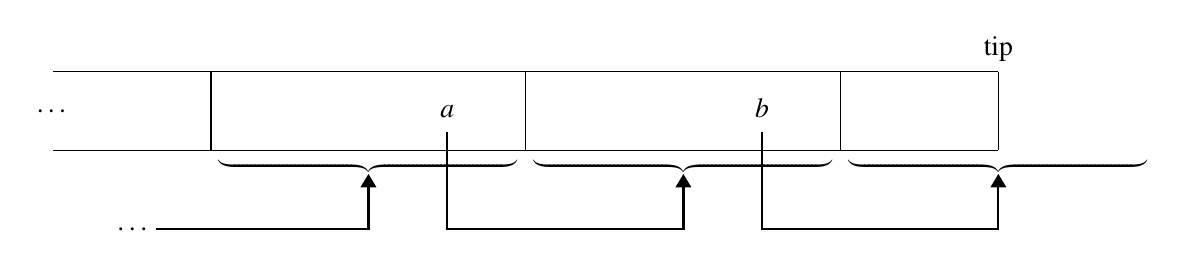
\begin{tikzpicture}
%                             /--------\
%                             |        |
%                             *        v  tip
% 1 -----+------------+------------+-----+
%        |       *    |            |     * current stake
% 0 -----+------------+------------+-----|
%   -10  -8           -4           0     2
%                |          ^
%                \----------/
\draw (-10, 0.5) node{\ldots};
\draw (-10,  0) --  (2, 0);
\draw (-10,  1) --  (2, 1);
\draw  (-8,  0) -- (-8, 1);
\draw  (-4,  0) -- (-4, 1);
\draw   (0,  0) --  (0, 1);
\draw   (2,  0) --  (2, 1) node[above]{tip};
\draw  (-6, -0.2) node {$\underbrace{\hspace{3.8cm}}$};
\draw  (-2, -0.2) node {$\underbrace{\hspace{3.8cm}}$};
\draw  ( 2, -0.2) node {$\underbrace{\hspace{3.8cm}}$};
\draw [thick, arrows={-Triangle}] (-9, -1) node[fill=white] {$\ldots$}-- (-6, -1) -- (-6, -0.3);
\draw [thick, arrows={-Triangle}] (-5, 0.5) node[fill=white] {$\mathstrut a$} -- (-5, -1) -- (-2, -1) -- (-2, -0.3);
\draw [thick, arrows={-Triangle}] (-1, 0.5) node[fill=white] {$\mathstrut b$} -- (-1, -1) -- (2, -1) -- (2, -0.3);
\end{tikzpicture}
\end{center}
%
This makes it possible to \emph{forecast} what the stake distribution (i.e.,
the ledger view) will be at various points. For example, if the chain looks like
%
\begin{center}
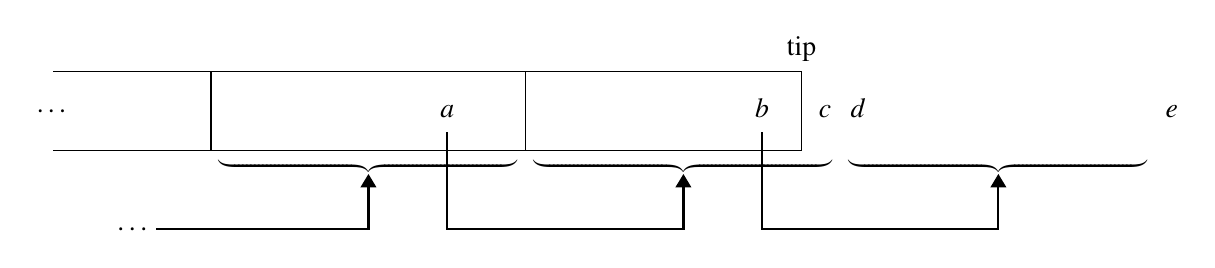
\begin{tikzpicture}
\draw (-10,    0.5) node{\ldots};
\draw (-10,    0) -- (-0.5, 0);
\draw (-10,    1) -- (-0.5, 1);
\draw  (-8,    0) -- (-8,   1);
\draw  (-4,    0) -- (-4,   1);
\draw  (-0.5,  0) -- (-0.5, 1) node[above]{tip};
\draw  (-6,   -0.2) node {$\underbrace{\hspace{3.8cm}}$};
\draw  (-2,   -0.2) node {$\underbrace{\hspace{3.8cm}}$};
\draw  ( 2,   -0.2) node {$\underbrace{\hspace{3.8cm}}$};
\draw [thick, arrows={-Triangle}] (-9, -1) node[fill=white] {$\ldots$}-- (-6, -1) -- (-6, -0.3);
\draw [thick, arrows={-Triangle}] (-5, 0.5) node[fill=white] {$\mathstrut a$} -- (-5, -1) -- (-2, -1) -- (-2, -0.3);
\draw [thick, arrows={-Triangle}] (-1, 0.5) node[fill=white] {$\mathstrut b$} -- (-1, -1) -- (2, -1) -- (2, -0.3);
\draw (0, 0.5) node[left] {$\mathstrut c$};
\draw (0, 0.5) node[right] {$\mathstrut d$};
\draw (4, 0.5) node[right] {$\mathstrut e$};
\end{tikzpicture}
\end{center}
%
then we can ``forecast'' that the stake distribution at point $c$ will be the one
established at point $a$, whereas the stake distribution at point $d$ will be the
one established at point $b$. The stake distribution at point $e$ is however not
yet known; we say that $e$ is ``out of the forecast range''.

\subsection{Code}

Since we're always forecasting what the ledger would look like \emph{if it would
be advanced to a particular slot}, the result of forecasting is always something
ticked:\footnote{An \emph{unticked} ledger view would arise from deriving the
ledger view from the \emph{current} ledger state, not taking (nor needing to
take) into account any changes that have been scheduled for later slots. The
unticked ledger view is however rarely useful; when we validate a header, any
changes that have been scheduled in the most recent ledger state for slots
before or at the slot number of the header must be applied before we validate
the header; we therefore almost exclusively work with ticked ledger views.}
%
\begin{lstlisting}
data Forecast a = Forecast {
      forecastAt  :: WithOrigin SlotNo
    , forecastFor :: SlotNo -> Except OutsideForecastRange (Ticked a)
    }
\end{lstlisting}
%
Here \lstinline!forecastAt! is the tip of the ledger in which the forecast was
constructed and \lstinline!forecastFor! is constructing the forecast for a
particular slot, possibly returning an error message of that slot is out of
range. This terminology---a forecast constructed \emph{at} a slot
and computed \emph{for} a slot---is used throughout both this technical report
as well as the consensus layer code base.

\subsection{Ledger view}
\label{forecast:ledgerview}

For the ledger view specifically, the \lstinline!LedgerSupportsProtocol!
class (\cref{ledger:api:LedgerSupportsProtocol}) requires a function
%
\begin{lstlisting}
ledgerViewForecastAt ::
     LedgerConfig blk
  -> LedgerState blk
  -> Forecast (LedgerView (BlockProtocol blk))
\end{lstlisting}
%
This function must satisfy two important properties:
%
\begin{description}
\item[Sufficient range]

When we validate headers from an upstream node, the most recent usable ledger
state we have is the ledger state at the intersection of our chain and the chain
of the upstream node. That intersection will be at most $k$ blocks back, because
that is our maximum rollback and we disconnect from nodes that fork from our
chain more than $k$ blocks ago (\cref{consensus:overview:k}). Furthermore, it is
only useful to track an upstream peer if we might want to adopt their blocks,
and we only switch to their chain if it is longer than ours
(\cref{consensus:overview:chainsel}). This means that in the worst case
scenario, with the intersection $k$ blocks back, we need to be able to evaluate
$k + 1$ headers in order to adopt the alternative chain. However, the range of a
forecast is based on \emph{slots}, not blocks; since not every slot may contain
a block (\cref{time:slots-vs-blocks}), the range needs to be sufficient to
\emph{guarantee} to contain at least $k + 1$ blocks\footnote{Due to a
misalignment between the consensus requirements and the Shelley specification,
this is not the case for Shelley, where the effective maximum rollback is in
fact $k - 1$; see \cref{shelley:forecasting}).}; we will come back to this in
\cref{future:block-vs-slot}.

The network layer may have additional reasons for wanting a long forecast
range; see \cref{nonfunctional:network:headerbody}.

\item[Relation to ticking]
Forecasting is not the only way that we can get a ledger view for a particular
slot; alternatively, we can also \emph{tick} the ledger state, and then ask
for the ledger view at that ticked ledger state. These two ways should give us
the same answer:
%
\begin{equation}
\begin{array}{lllll}
\mathrm{whenever} &
\mathtt{forecastFor} \; (\mathtt{ledgerViewForecastAt}_\mathit{cfg} \; l) \; s & = & \mathtt{Right} & l' \\
\mathrm{then} & \mathtt{protocolLedgerView}_\mathit{cfg} \; (\mathtt{applyChainTick}_\mathit{cfg} \; s \; l) & = && l'
\end{array}
\end{equation}
%
In other words, whenever the ledger view for a particular slot is within the
forecast range, then ticking the ledger state to that slot and asking for the
ledger view at the tip should give the same answer. Unlike forecasting, however,
ticking has no maximum range. The reason is the following fundamental difference between these two concepts:
%
\begin{quote}
\textbf{(Forecast vs. ticking)} When we \emph{forecast} a ledger view, we are
predicting what that ledger view will be, \emph{no matter which blocks will  be
applied to the chain} between the current tip and the slot of the forecast. By
contrast, when we \emph{tick} a ledger, we are applying any time-related
changes to the ledger state in order to apply the \emph{next} block; in other
words, when we tick to a particular slot, \emph{there \emph{are} no blocks in
between the current tip and the slot we're ticking to}. Since there are no
intervening blocks, there is no uncertainty, and hence no limited range.
\end{quote}
\end{description}

\section{Queries}
\label{ledger:queries}

\section{Abandoned approach: historical states}

\chapter{Serialisation abstractions}
\label{serialisation}

Some of the various pieces of data that are handled by consensus also need to be
serialised to a binary format so that they can be:

\begin{enumerate}
\item written/read to/from \emph{storage} (see \cref{storage}) or;
\item sent/received across the \emph{network} (e.g., headers via the chain sync
  protocol \cref{chainsyncclient}).
\end{enumerate}

The two serialisation purposes above have different requirements and are
independent of each other. For example, when establishing a network connection,
a version number is negotiated. We can vary the network serialisation format
depending on the version number, allowing for instance to include some more
information in the payload. A concrete example of this is that starting from a
certain version, we include the block size in the payload when sending a
Byron\todo{Can I talk about Byron here?} header across the network as the header
itself does not contain it. This kind of versioning only concerns the network
and is independent of the storage layer. Hence we define separate abstractions
for them, decoupling them from each other.

For both abstractions, we use the CBOR (Concise Binary Object
Representation)\todo{command for acronyms?} format, because it has the following
benefits, paraphrasing the \texttt{cborg} library\todo{link?}:
\begin{itemize}
\item fast serialisation and deserialisation
\item compact binary format
\item stable format across platforms (32/64bit, big/little endian)
\item potential to read the serialised format from other languages
\item incremental or streaming (de)serialisation
\item suitable to use with untrusted input (resistance to asymmetric resource consumption attacks)
\item ...
\end{itemize}
Moreover, CBOR was chosen for the initial implementation of the Cardano
blockchain,\todo{correct?} with which we must maintain binary compatibility.
While it was possible to switch to another format for the block types developed
after the initial implementation, we saw no reason to switch.

We will now discuss both serialisation abstractions in more detail.

\section{Serialising for storage}
\label{serialisation:storage}

The following data is stored on disk (see \cref{storage}):

\begin{itemize}
\item Blocks
\item The extended ledger state (see \cref{storage:extledgerstate} and
  \cref{ledgerdb:on-disk}) which is the combination of:
  \begin{itemize}
  \item The header state (\cref{storage:headerstate})
  \item The ledger state\todo{link?}
  \end{itemize}
\end{itemize}

We use the following abstraction for serialising data to and from disk:

\begin{lstlisting}
class EncodeDisk blk a where
  encodeDisk :: CodecConfig blk -> a -> Encoding

class DecodeDisk blk a where
  decodeDisk :: CodecConfig blk -> forall s. Decoder s a
\end{lstlisting}

\begin{itemize}
\item These type classes have two type parameters: the block \lstinline!blk!,
  over which most things are parameterised, and \lstinline!a!, the type to
  (de)serialise. For example, \lstinline!a! can be the block type itself or the
  type corresponding to the ledger state.
\item \lstinline!CodecConfig blk! is a data family that defines the extra
  configuration needed for (de)serialisation. For example, to deserialise an EBB
  (\cref{ebbs}), the number of slots per epoch needs to be known statically to
  compute the slot of the block based on the epoch number, as the serialisation
  of an EBB does not contain its slot number, but the in-memory representation
  does. This configuration is kept as small as possible and is ideally empty.
\item The \lstinline!a -> Encoding! and \lstinline!forall s. Decoder s a! are
  the types for respectively encoders and decoders of the \lstinline!cborg!
  library.\todo{link?}
\item The encoder and decoder are split in two classes because they are not
  always \emph{symmetric}: the instantiation of \lstinline!a! in the encoder is
  not always the same as in the corresponding decoder. This is because blocks
  are \emph{annotated} with their serialisation. We discuss this in more detail
  in \cref{serialisation:annotations}.
\end{itemize}

\subsection{Nested contents}
\label{serialisation:storage:nested-contents}

By writing a block to disk we automatically have written the block's header to
disk, as the header is a part of the block. While we never write just a header,
we do support \emph{reading} just the header. This is more efficient than
reading the entire block and then extracting the header, as fewer bytes have to
be read from disk and deserialised.

\begin{center}
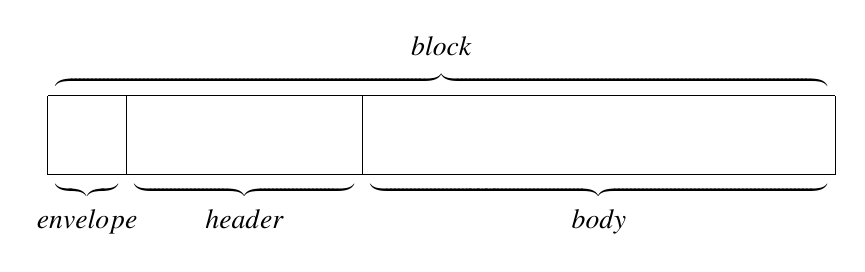
\begin{tikzpicture}
\draw  (0,    0)  -- (10,  0);
\draw  (0,    1)  -- (10,  1);
\draw  (0,    0)  --  (0,  1);
\draw  (1,    0)  --  (1,  1);
\draw  (4,    0)  --  (4,  1);
\draw (10,    0)  -- (10,  1);
\draw  (5,    1.2) node {$\overbrace{\hspace{9.8cm}}$};
\draw  (5,    1.6) node[fill=white] {$\mathstrut block$};
\draw  (0.5, -0.2) node {$\underbrace{\hspace{0.8cm}}$};
\draw  (0.5, -0.6) node[fill=white] {$\mathstrut envelope$};
\draw  (2.5, -0.2) node {$\underbrace{\hspace{2.8cm}}$};
\draw  (2.5, -0.6) node[fill=white] {$\mathstrut header$};
\draw  (7,   -0.2) node {$\underbrace{\hspace{5.8cm}}$};
\draw  (7,   -0.6) node[fill=white] {$\mathstrut body$};
\end{tikzpicture}
\end{center}

Extracting the header from a block on disk can be very simple, like in the
figure above. The block starts with an envelope, which is followed by the block
header and the block body. In this case, we read the bytes starting from the
start of the header until the end of the header, which we then decode. We use
the following abstraction to represent this information:

\begin{lstlisting}
data BinaryBlockInfo = BinaryBlockInfo {
      headerOffset :: !Word16
    , headerSize   :: !Word16
    }

class HasBinaryBlockInfo blk where
  getBinaryBlockInfo :: blk -> BinaryBlockInfo
\end{lstlisting}

As the size of a header can vary on a per-block basis, we maintain this
information \emph{per block} in the storage layer.\todo{link?} We trade four
extra bytes of storage and memory space for faster reading of headers.

However, it is not for every type of block the case that the encoding of a
header can literally be sliced out of the encoding of the corresponding block.
The serialisation of a header when embedded in a block might be different from
the serialisation of a header on its own. For example, the standalone header
might require an additional envelope or a different one than the block's
envelope.

A concrete example of this are the Byron blocks and headers. A Byron block is
either a regular block or an epoch boundary block (EBB) (discussed in
\cref{ebbs}). A regular block has a different header than an EBB, consequently,
their encoding differs. The envelope of the encoding of a Byron block includes a
tag indicating whether the block is a regular block or an EBB, so that the
decoder knows what kind of header and body to expect. For the same reason, the
envelope of the encoding of a standalone Byron header includes the same tag.
However, when we slice out the header from the Byron block and feed that to the
decoder for Byron headers, the envelope containing the tag will be
\emph{missing}.

The same problem presents itself for the hard fork combinator (\cref{hfc}): when
using the hard fork combinator to combine two block types, A and B, into one,
the block's envelope will (typically) indicate whether it is a block of type A
or B. The header corresponding to such a block will have a similar envelope.
When we slice the header out of such a block, the required envelope will be
missing. The right envelope has to be prepended so that the header decoder knows
whether it should expect A or B.

The header is \emph{nested} inside the block and to be able to decode it, we
need some more \emph{context}, i.e., the envelope of the header. In the storage
layer (\cref{storage}), we store the context of each block in an index
(in-memory or on-disk, depending on the database) so that after reading both the
context and the sliced header, we can decode the header without having to read
and decode the entire block. We capture this idea in the following abstractions.

\begin{lstlisting}
data family NestedCtxt_ blk :: (Type -> Type) -> (Type -> Type)
\end{lstlisting}
As usual, we parameterise over the block type. We also parameterise over another
functor, e.g., \lstinline!f!, which in practice will be instantiated to
\lstinline!Header!, but in the future, there might be more types of nested
contents, other than headers, e.g., block bodies. The constructors of this data
family will represent the different types of context available, e.g., for Byron
a context for regular blocks and a context for EBBs.

\lstinline!NestedCtxt! is indexed by \lstinline!blk!: it is the block that
determines this type. However, we often want to partially apply the second
argument (the functor), leaving the block type not yet defined, hence we define:
\begin{lstlisting}
newtype NestedCtxt f blk a = NestedCtxt {
      flipNestedCtxt :: NestedCtxt_ blk f a
    }
\end{lstlisting}
The \lstinline!a! type index will correspond to the raw, sliced header that
requires the additional context. It can vary with the context, e.g., the context
for a Byron EBB will fix \lstinline!a! to a raw EBB header (without the
necessary envelope).

Now that we have defined \lstinline!NestedCtxt!, we can define the class that
allows us to separate the nested type (the header) into the context and the raw,
sliced type (the raw header, \lstinline!a!), as well as the inverse:
\begin{lstlisting}
class (..) => HasNestedContent f blk where
  unnest :: f blk -> DepPair (NestedCtxt f blk)
  nest   :: DepPair (NestedCtxt f blk) -> f blk
\end{lstlisting}
\lstinline!DepPair! is a dependent pair that allows us to hide the type
parameter \lstinline!a!. When writing a block, \lstinline!unnest! is used to
extract the context so that it can be stored in the appropriate index. When
reading a header, \lstinline!nest! is used to combine the context, read from the
appropriate index, with the raw header into the header.

In certain scenarios, we do not have access to the separately stored context of
the block, but we do have access to the encoded block, in which case we should
be able to able to extract the context directly from the encoded block, without
having to decode it entirely. We use the \lstinline!ReconstructNestedCtxt! class
for this:
\begin{lstlisting}
class HasNestedContent f blk => ReconstructNestedCtxt f blk where
  reconstructPrefixLen  :: proxy (f blk) -> PrefixLen
  reconstructNestedCtxt ::
       proxy (f blk)
    -> ShortByteString
    -> ..
    -> SomeSecond (NestedCtxt f) blk
\end{lstlisting}
The \lstinline!PrefixLen! is the number of bytes extracted from the beginning of
the encoded block required to reconstruct the context. The
\lstinline!ShortByteString! corresponds to these bytes. The
\lstinline!reconstructNestedCtxt! method will parse this bytestring and return
the corresponding context. The \lstinline!SomeSecond! type is used to hide the
type parameter \lstinline!a!.

As these contexts and context-dependent types do not fit the mould of the
\lstinline!EncodeDisk! and \lstinline!DecodeDisk! classes described in
\cref{serialisation:storage}, we define variants of these classes:
\begin{lstlisting}
class EncodeDiskDepIx f blk where
  encodeDiskDepIx :: CodecConfig blk
                  -> SomeSecond f blk -> Encoding

class DecodeDiskDepIx f blk where
  decodeDiskDepIx :: CodecConfig blk
                  -> Decoder s (SomeSecond f blk)

class EncodeDiskDep f blk where
  encodeDiskDep :: CodecConfig blk -> f blk a
                -> a -> Encoding

class DecodeDiskDep f blk where
  decodeDiskDep :: CodecConfig blk -> f blk a
                -> forall s. Decoder s (ByteString -> a)
\end{lstlisting}
\todo{explain?}

\section{Serialising for network transmission}
\label{serialisation:network}

The following data is sent across the network:
\begin{itemize}
\item Header hashes
\item Blocks
\item Headers
\item Transactions
\item Transaction IDs
\item Transaction validation errors
\item Ledger queries
\item Ledger query results
\end{itemize}
\todo{less whitespace}

We use the following abstraction for serialising data to and from the network:

\begin{lstlisting}
class SerialiseNodeToNode blk a where
  encodeNodeToNode :: CodecConfig blk
                   -> BlockNodeToNodeVersion blk
                   -> a -> Encoding
  decodeNodeToNode :: CodecConfig blk
                   -> BlockNodeToNodeVersion blk
                   -> forall s. Decoder s a

class SerialiseNodeToClient blk a where
  encodeNodeToClient :: CodecConfig blk
                     -> BlockNodeToClientVersion blk
                     -> a -> Encoding
  decodeNodeToClient :: CodecConfig blk
                     -> BlockNodeToClientVersion blk
                     -> forall s. Decoder s a
\end{lstlisting}

These classes are similar to the ones used for storage
(\cref{serialisation:storage}), but there are some important differences:

\begin{itemize}
\item The encoders and decoders are always symmetric, which means we do not have
  to separate encoders from decoders and can merge them in a single class.
  Nevertheless, some of the types sent across the network still have to deal
  with annotations (\cref{serialisation:annotations}), we discuss how we solve
  this in \cref{serialisation:network:cbor-in-cbor}.
\item We have separate classes for \emph{node-to-node} and \emph{node-to-client}
  serialisation.\todo{link?}
  By separating them, we are more explicit about which data is serialised for
  which type of connection. Node-to-node protocols and node-to-client protocols
  have different properties and requirements. This also gives us the ability to,
  for example, use a different encoding for blocks for node-to-node protocols
  than for node-to-client protocols.
\item The methods in these classes all take a \emph{version} as argument. We
  will discuss versioning in \cref{serialisation:network:versioning}.
\end{itemize}

\subsection{Versioning}
\label{serialisation:network:versioning}

As requirements evolve, features are added, data types change, constructors are
added and removed. For example, adding the block size to the Byron headers,
adding new ledger query constructors, etc. This affects the data we send across
the network. In a distributed network of nodes, it is a given that not all nodes
will simultaneously upgrade to the latest released version and that nodes
running different versions of the software, i.e., different versions of the
consensus layer, will try to communicate with each other. They should of course
be able to communicate with each other, otherwise the different versions would
cause partitions in the network.

This means we should be careful to maintain binary compatibility between
versions. The network layer is faced with the same issue: as requirements
evolve, network protocols (block fetch, chain sync\todo{link?}) are modified
change (adding messages, removing messages, etc.), network protocols are added
or retired, etc. While the network layer is responsible for the network
protocols and the encoding of their messages, the consensus layer is responsible
for the encoding of the data embedded in these messages. Changes to either
should be possible without losing compatibility: a node should be able to
communicate successfully with other nodes that run a newer or older version of
the software, up to certain limits (old versions can be retired eventually).

To accomplish this, the network layer uses \emph{versions}, one for each bundle
of protocols:
\begin{lstlisting}
data NodeToNodeVersion
    = NodeToNodeV_1
    | NodeToNodeV_2
    | ..

data NodeToClientVersion
    = NodeToClientV_1
    | NodeToClientV_2
    | ..
\end{lstlisting}
For each backwards-incompatible change, either a change in the network protocols
or in the encoding of the consensus data types, a new version number is
introduced in the corresponding version data type. When the network layer
establishes a connection with another node or client, it will negotiate a
version number during the handshake: the highest version that both parties can
agree on. This version number is then passed to any client and server handlers,
which decide based on the version number which protocols to start and which
protocol messages (not) to send. A new protocol message would only be sent when
the version number is greater or equal than the one with which it was
introduced.

This same network version is passed to the consensus layer, so we can follow the
same approach. However, we decouple the network version numbers from the
consensus version numbers for the following reason. A new network version number
is needed for each backwards-incompatible change to the network protocols or the
encoding of the consensus data types. This is clearly a strict superset of the
changes caused by consensus. When the network layer introduces a new protocol
message, this does not necessarily mean anything changes in the encoding of the
consensus data types. This means multiple network versions can correspond to the
same consensus-side encoding or \emph{consensus version}. In the other
direction, each change to the consensus-side encodings should result in a new
network version. We capture this in the following abstraction:
\begin{lstlisting}
class (..) => HasNetworkProtocolVersion blk where
  type BlockNodeToNodeVersion   blk :: Type
  type BlockNodeToClientVersion blk :: Type

class HasNetworkProtocolVersion blk
   => SupportedNetworkProtocolVersion blk where
  supportedNodeToNodeVersions ::
       Proxy blk -> Map NodeToNodeVersion   (BlockNodeToNodeVersion   blk)
  supportedNodeToClientVersions ::
       Proxy blk -> Map NodeToClientVersion (BlockNodeToClientVersion blk)
\end{lstlisting}
The \lstinline!HasNetworkProtocolVersion! class has two associated types to
define the consensus version number types for the given block. When no
versioning is needed, one can use the unit type as the version number. The
\lstinline!SupportedNetworkProtocolVersion! defines the mapping between the
network and the consensus version numbers. Note that this does not have to be an
injection, as multiple network version can most certainly map to the same
consensus version. Nor does this have to be a surjection, as old network and
consensus versions might be removed from the mapping when the old version no
longer needs to be supported. This last reason is also why this mapping is
modelled with a \lstinline!Map! instead of a function: it allows enumerating a
subset of all defined versions, which is not possible with a function.

\todo{TODO} Global numbering vs multiple block types

The \lstinline!SerialiseNodeToNode! and \lstinline!SerialiseNodeToClient!
instances can then branch on the passed version to introduce changes to the
encoding format, for example, the inclusion of the block size in the Byron
header encoding.

Consider the following scenario: a change is made to one of the consensus data
types, for example, a new query constructor is added the ledger query data type.
This requires a new consensus and thus network version number, as older versions
will not be able to decode it. What should be done when the new query
constructor is sent to a node that does not support it (the negotiated version
is older than the one in which the constructor was added)? If it is encoded and
send, the receiving side will fail to decode it and terminate its
connection.\todo{right?} This is rather confusing to the sender, as they are
left in the dark. Instead, we let the \emph{encoder} throw an exception in this
case, terminating that connection, so that the sender is at least notified of
this. \todo{TODO} Ideally, we could statically prevent such cases.

\subsection{CBOR-in-CBOR}
\label{serialisation:network:cbor-in-cbor}

In \cref{serialisation:annotations}, we explain why the result of the decoder
for types using \emph{annotations} needs to be passed the original encoding as a
bytestring. When reading from disk, we already have the entire bytestring in
memory,\todo{explain why} so it can easily be passed to the result of the
decoder. However, this is not the case when receiving a message via the network
layer: the entire message, containing the annotated type(s), is decoded
incrementally.\todo{right?} When decoding CBOR, it is not possible to obtain the
bytestring corresponding to what the decoder is decoding. To work around this,
we use \emph{CBOR-in-CBOR}: we encode the original data as CBOR and then encode
the resulting bytestring as CBOR \emph{again}. When decoding CBOR-in-CBOR, after
decoding the outer CBOR layer, we have exactly the bytestring that we will need
for the annotation. Next, we feed this bytestring to the original decoder, and,
finally, we pass the bytestring to the function returned by the decoder.

\subsection{Serialised}
\label{serialisation:network:serialised}

One of the duties of the consensus layer is to serve blocks and headers to other
nodes in the network.\todo{link?} To serve for example a block, we read it from
disk, deserialise it, and then serialise it again and send it across the
network. The costly deserialisation and serialisation steps cancel each other
out and are thus redundant. We perform this optimisation in the following way.
When reading such a block from storage, we do not read the \lstinline!blk!, but
the \lstinline!Serialised blk!, which is a phantom type around a raw, still
serialised bytestring:
\begin{lstlisting}
newtype Serialised a = Serialised ByteString
\end{lstlisting}
To send this serialised block over the network, we have to encode this
\lstinline!Serialised blk!. As it happens, we use CBOR-in-CBOR to send both
blocks and headers over the network, as described in
\cref{serialisation:network:cbor-in-cbor}. This means the serialised block
corresponds to the inner CBOR layer and that we only have to encode the
bytestring again as CBOR, which is cheap.

This optimisation is only used to \emph{send} and thus encode blocks and
headers, not when \emph{receiving} them, because each received block or header
will have to be inspected and validated, and thus deserialised anyway.

As discussed in \cref{serialisation:storage:nested-contents}, reading a header
(nested in a block) from disk requires reading the context and the raw header,
and then combining them before we can deserialise the header. This means the
approach for serialised headers differs slightly:
\begin{lstlisting}
newtype SerialisedHeader blk = SerialisedHeaderFromDepPair {
      serialisedHeaderToDepPair :: GenDepPair Serialised
                                              (NestedCtxt Header blk)
    }
\end{lstlisting}
This is similar to the \lstinline!DepPair (NestedCtxt f blk)! type from
\cref{serialisation:storage:nested-contents}, but this time the raw header is
wrapped in \lstinline!Serialised! instead of being deserialised.

\section{Annotations}
\label{serialisation:annotations}

\todo{TODO} move up? The previous two sections refer to this

The following technique is used in the Byron and Shelley ledgers for a number of
data types like blocks, headers, transactions, \ldots The in-memory representation
of, for example a block, consists of both the typical fields describing the
block (header, transactions, \ldots), but also the \emph{serialisation} of the block
in question. The block is \emph{annotated} with its serialisation.

The principal reason for this is that it is possible that multiple
serialisations, each which a different hash, correspond to the same logical
block. For example, a client sending us the block might encode a number using a
binary type that is wider than necessary (e.g., encoding the number 0 using four
bytes instead of a single byte). CBOR defines a \emph{canonical format}, we call
an encoding that is in CBOR's canonical format a \emph{canonical
encoding}.\todo{link?}

When after deserialising a block in a non-canonical encoding, we serialise it
again, we will end up with a different encoding, i.e., the canonical encoding,
as we stick to the canonical format. This means the hash, which is part of the
blockchain, is now different and can no longer be verified.

For this reason, when deserialising a block, the original, possibly
non-canonical encoding is retained and used to annotate the block. To compute
the hash of the block, one can hash the annotated serialisation.

Besides solving the issue with non-canonical encodings, this has a performance
advantage, as encoding such a block is very cheap, it is just a matter of
copying the in-memory annotation.

\todo{TODO} We rely on it being cheap in a few places, mention that/them?

\todo{TODO} extra memory usage

This means that the result of the decoder must be passed the original encoding
as a bytestring to use as the annotation of the block or other type in question.
Hence the decoder corresponding to the encoder \lstinline!blk -> Encoding! has
type \lstinline!forall s. Decoder s (ByteString -> blk)!, which is a different
instantiation of the type \lstinline!a!, explaining the split of the
serialisation classes used for storage (\cref{serialisation:storage}). The
original encoding is then applied to the resulting function to obtain the
annotated block. This asymmetry is handled in a different way for the network
serialisation, namely using CBOR-in-CBOR
(\cref{serialisation:network:cbor-in-cbor}).

\subsection{Slicing}

\todo{TODO} discuss the slicing of annotations with an example. What is the
relation between the decoded bytestring and the bytestring passed to the
function the decoder returns? Talk about compositionality.


\part{Storage Layer}

\chapter{Overview}
\label{storage}

\section{Components}
\label{storage:components}

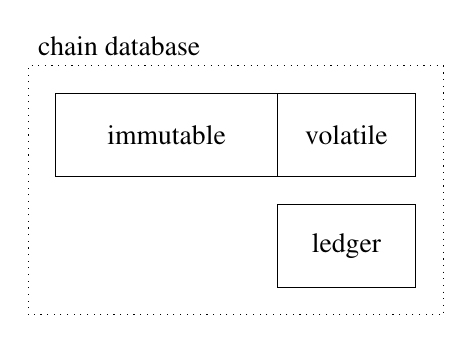
\begin{tikzpicture}
\draw [dotted]
     (-50pt, -65pt)
  -- ++(0, 90pt) node[above right] {chain database}
  -- ++(150pt, 0)
  -- ++(0, -90pt)
  -- cycle;
\node [draw, shape=rectangle, minimum width=80pt, minimum height=30pt] at (0,0)  {immutable};
\node [draw, shape=rectangle, minimum width=50pt, minimum height=30pt] at (65pt, 0)  {volatile};
\node [draw, shape=rectangle, minimum width=50pt, minimum height=30pt] at (65pt, - 40pt) {ledger};
\end{tikzpicture}

Discuss the immutable/volatile split (we reference this section for that).

\section{In memory}
\label{storage:inmemory}

TODO: After we discussed the overview, we should give an overview of everything
we store in memory in any component, so that we have a better understanding of
memory usage of the chain DB as a whole.

\subsection{Chain fragments}
\label{storage:fragments}

\subsection{Extended ledger state}
\label{storage:extledgerstate}
\label{storage:headerstate}

TODO: Is there a more natural place to talk about this? Introducing the
header state when introducing the storage layer does not feel quite right.
The storage layer might be storing the header state, but that doesn't
explain its existence.

ChainDepState, (ChainIndepState), LedgerState, ExtLedgerState

\newcommand{\chunkNumber}[1]{\ensuremath{\mathsf{chunkNumber}(#1)}}
\newcommand{\relativeSlot}[2]{\ensuremath{\mathsf{relativeSlot}(#1, #2)}}

\chapter{Immutable Database}
\label{immutable}

The Immutable DB is tasked with storing the blocks that are part of the
\emph{immutable} part of the chain. Because of the nature of this task, the
requirements and \emph{non-requirements} of this component are fairly specific:

\begin{itemize}
\item \textbf{Append-only}: as it represents the immutable chain, blocks will
  only be appended in the same order as they are ordered in the chain. Blocks
  will never be \emph{modified} or \emph{deleted}.
\item \textbf{Reading}: the database should be able to return the block or
  header stored at a given \emph{point} (combination of slot number and hash)
  efficiently.\todo{define point somewhere?}
\item \textbf{Efficient streaming}: when serving blocks or headers to other
  nodes, we need to be able to stream ranges of \emph{consecutive} blocks or
  headers efficiently. As described in \cref{serialisation:network:serialised},
  it should be possible to stream \emph{raw} blocks and headers, without
  serialising them.
\item \textbf{Recoverability}: it must be possible to validate the blocks stored
  in the database. When a block in the database is corrupt or missing, it is
  sufficient to truncate the database, representing an immutable chain, to the
  last valid block before the corrupt or missing block. The truncated blocks can
  simply be downloaded again. It is therefore not necessary to be able recover
  the full database when blocks are missing.
\end{itemize}

While we touched upon some of the non-requirements already above, it is useful
to highlight the following non-requirements.

\begin{itemize}
\item \textbf{Queries}: besides looking up a single block by its point and
  streaming ranges of consecutive blocks, the database does have to be able to
  answer queries about blocks. No searching or filtering is needed.
\item \textbf{Durability}: the system does not require the durability guarantee
  that traditional database systems provide (the D in ACID). If the system
  crashes right after appending a block, it is acceptable that the block in
  question is truncated when recovering the database. Because of the overlap
  with the Volatile DB\todo{link}, such a truncation is likely to even go
  unnoticed. In the worst case, the truncated blocks can simply be downloaded
  again.
\end{itemize}

Because of the specific requirements and non-requirements listed above, we
decided to write our own implementation, the \lstinline!ImmutableDB!, instead of
using an existing off-the-shelf database system. Traditional database systems
provide guarantees that are not needed and, conversely, do not take advantage of
the requirements to optimise certain operations. For example, there is no need
for a journal or flushing (\lstinline!fsync!) the buffers after each write
because of our unique durability and recoverability (non-)requirements.

\section{API}
\label{immutable:api}

Before we describe the implementation of the Immutable DB, we first describe its
functionality. The Immutable DB has the following API:

\begin{lstlisting}
data ImmutableDB m blk = ImmutableDB {
      closeDB :: m ()

    , getTip :: STM m (WithOrigin (Tip blk))

    , appendBlock :: blk -> m ()

    , getBlockComponent ::
           forall b.
           BlockComponent blk b
        -> RealPoint blk
        -> m (Either (MissingBlock blk) b)

    , stream ::
           forall b.
           ResourceRegistry m
        -> BlockComponent blk b
        -> StreamFrom blk
        -> StreamTo   blk
        -> m (Either (MissingBlock blk) (Iterator m blk b))
    }
\end{lstlisting}

The database is parameterised over the block type \lstinline!blk! and the monad
\lstinline!m!, like most of the consensus layer.\todo{mention io-sim}
\todo{TODO} Mention our use of records for components?

The \lstinline!closeDB! operation closes the database, allowing all opened
resources, including open file handles, to be released. This is typically only
used when shutting down the entire system. Calling any other operation on an
already-closed database should result in an exception.

The \lstinline!getTip! operation returns the current tip of the Immutable DB.
The \lstinline!Tip! type contains information about the block at the tip like
the slot number, the block number, the hash, etc. The \lstinline!WithOrigin!
type is isomorphic to \lstinline!Maybe! and is used to account for the
possibility of an empty database, i.e., when the tip is at the ``origin'' of the
chain. This operation is an \lstinline!STM! operation, which allows it to be
combined with other \lstinline!STM! operations in a single transaction, to
obtain a consistent view on them. This also implies that no IO or disk access is
needed to obtain the current tip.

The \lstinline!appendBlock! operation appends a block to the Immutable DB. As
slot numbers increase monotonically in the blockchain, the block's slot must be
greater than the current tip's slot (or equal when the tip points at an EBB, see
\cref{ebbs}). It is not required that each slot is filled,\todo{link?} so there
can certainly be gaps in the slot numbers.

The \lstinline!getBlockComponent! operation allows reading one or more
components of the block in the database at the given point. We discuss what
block components are in \cref{immutable:api:block-component}. The
\lstinline!RealPoint! type represents a point that can only refer to a block,
not to genesis (the empty chain), which the larger \lstinline!Point! type
allows. As the given point might not be in the Immutable DB, this operation can
also return a \lstinline!MissingBlock! error instead of the requested block
component.

The \lstinline!stream! operation returns an iterator to efficiently stream the
blocks between the two given bounds. The bounds are defined as such:
\begin{lstlisting}
data StreamFrom blk =
    StreamFromInclusive !(RealPoint blk)
  | StreamFromExclusive !(Point     blk)

newtype StreamTo blk =
    StreamToInclusive (RealPoint blk)
\end{lstlisting}
Lower bounds can be either inclusive or exclusive, but exclusive upper bounds
were omitted because they were not needed in practice. An inclusive bound must
refer to a block, not genesis, hence the use of \lstinline!RealPoint!. The
exclusive lower bound \emph{can} refer to genesis, hence the use of
\lstinline!Point!, in particular to begin streaming from the start of the chain.
As one or both of the bounds might not be in the Immutable DB, this operation
can return a \lstinline!MissingBlock! error. We discuss what block components
are in \cref{immutable:api:block-component}. The \lstinline!ResourceRegistry!
will be used to allocate all the resources the iterator opens during its
lifetime, e.g., file handles. By closing the registry in case of an exception
(using \lstinline!bracket!), all open resources are released and nothing is
leaked.\todo{link} More discussion about iterators follows in
\cref{immutable:api:iterators}.

\subsection{Block Component}
\label{immutable:api:block-component}

\todo{TODO} move to ChainDB?

Besides reading or streaming blocks from the Immutable DB, it must be possible
to read or stream headers, raw blocks (see
\cref{serialisation:network:serialised}), but in some cases also \emph{nested
contexts} (see \cref{serialisation:storage:nested-contents}) or even block
sizes. Adding an operation to the API for each of these would result in too much
duplication. We handle this with the \lstinline!BlockComponent! abstraction:
when reading or streaming, one can choose which \emph{components} of a block
should be returned, e.g., the block itself, the header of the block, the size of
the block, the raw block, the raw header, etc. We model this with the following
GADT:

\begin{lstlisting}
data BlockComponent blk a where
  GetVerifiedBlock :: BlockComponent blk blk
  GetBlock         :: BlockComponent blk blk
  GetRawBlock      :: BlockComponent blk ByteString
  GetHeader        :: BlockComponent blk (Header blk)
  GetRawHeader     :: BlockComponent blk ByteString
  GetHash          :: BlockComponent blk (HeaderHash blk)
  GetSlot          :: BlockComponent blk SlotNo
  GetIsEBB         :: BlockComponent blk IsEBB
  GetBlockSize     :: BlockComponent blk Word32
  GetHeaderSize    :: BlockComponent blk Word16
  GetNestedCtxt    :: BlockComponent blk (SomeSecond (NestedCtxt Header) blk)
  ..
\end{lstlisting}
The \lstinline!a! type index determines the type of the block component.
Additionally, we have \lstinline!Functor! and \lstinline!Applicative! instances.
The latter allows combining multiple \lstinline!BlockComponent!s into one. This
can be considered a small DSL for querying components of a block.

\subsection{Iterators}
\label{immutable:api:iterators}

The following API can be used to interact with an iterator:

\begin{lstlisting}
data Iterator m blk b = Iterator {
      iteratorNext    :: m (IteratorResult b)
    , iteratorHasNext :: STM m (Maybe (RealPoint blk))
    , iteratorClose   :: m ()
    }

data IteratorResult b =
    IteratorExhausted
  | IteratorResult b
\end{lstlisting}

The \lstinline!iteratorNext! operation returns the current
\lstinline!IteratorResult! and advances the iterator to the next block in the
stream. When the iterator has reached its upper bound, it is exhausted. Remember
that the \lstinline!b! type argument corresponds to the requested block
component.

The \lstinline!iteratorHasNext! operation returns the point corresponding to the
block the next call to \lstinline!iteratorNext! will return. When exhausted,
\lstinline!Nothing! is returned.

As an open iterator can hold onto resources, e.g., open file handles, it should
be explicitly closed using the \lstinline!iteratorClose! operation. Interacting
with a closed iterator should result in an exception, except for calling
\lstinline!iteratorClose!, which is idempotent.

\section{Implementation}
\label{immutable:implementation}

We will now give a high-level overview of our custom implementation of the
Immutable DB that satisfies the requirements and the API.

\begin{itemize}
\item We store blocks sequentially in a file, called a \emph{chunk file}. We
  append each raw block, without any extra information before or after it, to
  the chunk file. This will facilitate efficient binary streaming of blocks. In
  principle, it is a matter of copying bytes from one buffer to another, without
  any additional processing needed.

\item Every $x$ \emph{slots}, where $x$ is the configurable chunk size, we start
  a new chunk file to avoid storing all blocks in a single file.

\item To facilitate looking up a block by a point, which consists of the hash
  and the slot number, we ``index'' our database by slot numbers. One can then
  look up the block in the given slot and compare its hash against the point's
  hash. No searching will be needed.

  Blocks are stored sequentially in chunk files, but slot numbers do \emph{not}
  increase one-by-one; they are \emph{sparse}. This means we need a mapping from
  the slot number to the offset and size of the block in the chunk file. We
  store this mapping in the on-disk \emph{primary index}, one per chunk file,
  which we discuss in more detail in \cref{immutable:implementation:indices}.

\item As mentioned above, when looking up a block by a point, we will compare
  the hash of the block at the point's slot in the Immutable DB with the point's
  hash. We should be able to do this without first having to read and
  deserialise the entire block in order to know its hash.

  Moreover, it should be possible to read just the header of the block without
  first having to read the entire block. As described in
  \cref{serialisation:storage:nested-contents}, we can do this if have access to
  the header offset, header size, and nested context of the block.

  For these reasons, we store the aforementioned extra information, which should
  be available without having to read and deserialise the entire block,
  separately in the on-disk \emph{secondary index}, one per chunk file
  (\cref{immutable:implementation:indices}).

\item All the information stored in the primary and secondary indices can be
  recovered from the blocks in the chunk files. This is described in
  \cref{immutable:implementation:recovery}.

\item Whenever a file-system operation fails, or a file is missing or corrupted,
  we shut down the Immutable DB and consequently the whole system. When this
  happens, either the system's file system is no longer reliable (e.g., disk
  corruption), manual intervention (e.g., disk is full) is required, or there is
  a bug in the system. In all cases, there is no point in trying to continue
  operating. We shut down the system and flag the shutdown as \emph{dirty},
  triggering a full validation on the next start-up, see
  \cref{immutable:implementation:recovery}.

  Not all forms of disk corruption can easily be detected. For example, when
  some bytes in a block stored in a chunk file have been flipped on disk, this
  can easily go unnoticed. Deserialising the block might fail if the
  serialisation format is no longer valid, but the bitflip could also happen in,
  e.g., the amount of a transaction, which will not be detected by the
  deserialiser. In fact, the majority of blocks read will not even be
  deserialised, as blocks served to other nodes are read and sent in their raw,
  still serialised format. However, sending a corrupted block must be avoided,
  as nodes receiving it will consider it invalid and can blacklist us, mistaking
  us for an adversary.

  To detect such forms of silent corruption, we store CRC32 checksums in the
  secondary index (\cref{immutable:implementation:indices}) which we verify when
  reading the block, which we can do even when not deserialising the block. Note
  that we could use the block's own hash for this purpose,\footnote{To be
  precise: we would have to check the block body against the body hash stored in
  the header, and verify the signature of the header.} but because computing
  such a cryptographic hash is much more expensive, we opted for a separate
  CRC32 checksum, which is much more efficient to compute and designed for
  exactly this purpose.

\item We store the state of the current chunk, including its indices, in memory.
  We store this state, a pure data type, in a \lstinline!StrictMVar!. Besides
  avoiding space leaks by forcing its contents to WHNF, this
  \lstinline!StrictMVar! type has another useful ability that its standard
  non-strict variant is lacks: while it is locked when being modified, the
  previous, \emph{stale} value can still be read.

  This is convenient for the Immutable DB: we can support multiple concurrent
  reads even when at most one append operation is in progress, as it is safe to
  read a block based on the stale state because data will only be appended, not
  modified.

  To append a block to the Immutable DB, we lock the state to avoid concurrent
  append operations. We append the block to the chunk file, and append the
  necessary information to the primary and secondary indices. We unlock the
  state, updated with the information about the newly appended block.

\item We \emph{do not flush} any writes to disk, as discussed in the
  introduction of this chapter. This makes appending a block quite cheap: the
  serialised block is copied to an OS buffer, which is then asynchronously
  flushed in the background.

\item To avoid repeatedly reading and deserialising the same primary and
  secondary indices of older chunks, we cache them in a LRU-cache that is
  bounded in size.

\item To open an iterator, we check its bounds using the (cached) indices. The
  bounds are valid when both correspond to blocks present in the Immutable DB.
  Next, a file handle is opened for the chunk file containing the first block to
  stream. The same chunk file's indices are read (from the cache) and the
  iterator will maintain a list of secondary index entries, one for each block
  to stream from the chunk file. By having this list of entries in memory, the
  indices will not have to be accessed for each streamed block.

  When a block component is requested from the iterator, it is read from the
  chunk file and/or extracted from the corresponding in-memory entry.
  Afterwards, the entry is dropped from the in-memory list so that the next
  entry is ready to be read. When the list of entries is exhausted without
  reaching the end bound, we move on to the next chunk file. This process
  repeats until the end bound is reached.
\end{itemize}

\subsection{Chunk layout}
\label{immutable:implementation:chunk-layout}

Each block in the block chain has a unique slot number (except for EBBs, which
we discuss below). Slot numbers increase in the blockchain, but not all slots
have to be filled. For example, in the Byron era (using the Permissive BFT
consensus algorithm), nearly every slot will be filled, but in the Shelley era
(using the Praos consensus algorithm), on average only one in twenty slots will
be filled.

As mentioned above, we want to group blocks into chunk files. Because we need to
be able to look up blocks in the Immutable DB based on their slot number, we
group blocks into chunk files based on their slot numbers so that the chunk file
containing a block can be determined by looking at the slot number of the block.

Internally, we translate \emph{absolute} slot numbers into \emph{chunk numbers}
and \emph{relative slot numbers} (relative w.r.t.\ the chunk). As EBBs
(\cref{ebbs}) have the same slot number as their successor, this translation is
not injective. To restore injectivity, we include ``whether the block is an EBB
or not'' as an input to the translation.

\todo{TODO} how should this be formatted?

\begin{definition}[Chunk number]
  Let $s$ be the absolute slot number of a block. Using a chunk size of
  $\mathit{sz}$:

  \[
  \chunkNumber{s} = \lfloor s / \mathit{sz} \rfloor
  \]
  Naturally, chunks are zero-indexed.

\end{definition}

\begin{definition}[Relative slot number]
  Let $s$ be the absolute slot number of a block. Using a chunk size of
  $\mathit{sz}$:

  \[
  \relativeSlot{s}{\mathit{isEBB}} =
  \begin{cases}
    0                         & \text{if}\,\mathit{isEBB} \\
    (s \bmod \mathit{sz}) + 1 & \text{otherwise}
  \end{cases}
  \]
  We reserve the very first relative slot for an EBB, hence the need to make
  room for it by incrementing by one in the non-EBB case.
\end{definition}

In the example below, we show a chunk with chunk number 1 using a chunk size of
100:

\begin{center}
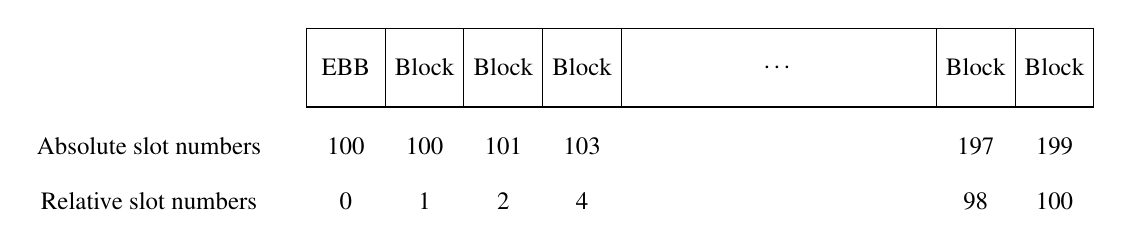
\begin{tikzpicture}
\draw (0, 0) -- (10, 0);
\draw (0, 1) -- (10, 1);

\draw ( 0, 0) -- ( 0, 1);
\draw ( 1, 0) -- ( 1, 1);
\draw ( 2, 0) -- ( 2, 1);
\draw ( 3, 0) -- ( 3, 1);
\draw ( 4, 0) -- ( 4, 1);
\draw ( 8, 0) -- ( 8, 1);
\draw ( 9, 0) -- ( 9, 1);
\draw (10, 0) -- (10, 1);

\draw (0.5, 0.5) node {\small EBB};
\draw (1.5, 0.5) node {\small Block};
\draw (2.5, 0.5) node {\small Block};
\draw (3.5, 0.5) node {\small Block};
\draw (6.0, 0.5) node {\small \ldots};
\draw (8.5, 0.5) node {\small Block};
\draw (9.5, 0.5) node {\small Block};

\draw (-2.0, -0.5) node {\small Absolute slot numbers};
\draw ( 0.5, -0.5) node {\small 100};
\draw ( 1.5, -0.5) node {\small 100};
\draw ( 2.5, -0.5) node {\small 101};
\draw ( 3.5, -0.5) node {\small 103};
\draw ( 8.5, -0.5) node {\small 197};
\draw ( 9.5, -0.5) node {\small 199};

\draw (-2.0, -1.2) node {\small Relative slot numbers};
\draw ( 0.5, -1.2) node {\small 0};
\draw ( 1.5, -1.2) node {\small 1};
\draw ( 2.5, -1.2) node {\small 2};
\draw ( 3.5, -1.2) node {\small 4};
\draw ( 8.5, -1.2) node {\small 98};
\draw ( 9.5, -1.2) node {\small 100};
\end{tikzpicture}
\end{center}
Note that some slots are empty, e.g., 102 and 198 are missing. The first and
lasts slots can be empty too. In practice, it will never be the case that an
entire chunk is empty, but the implementation allows for it.

If we were to pick a chunk size of 1 and store each block in its own file, we
would need millions of files, as there are millions of blocks. When serving
blocks to peer, we would constantly open and close individual block files, which
is very inefficient.

If we pick a very large or even unbounded chunk size, the resulting chunk file
would be several gigabytes in size and keep growing. This would make the
recovery process (\cref{immutable:implementation:recovery}) more complicated and
potentially much slower, as more data might have to be read and
validated.\todo{Other arguments?} Moreover, our current approach of caching
indices per chunk would have to be revised.

In practice, a chunk size of \num{21600} is used, which matches the \emph{epoch
size} of Byron. It is no coincidence that there is (at most) one EBB at the
start of each Byron epoch, fitting nicely in the first relative slot that we
reserve for it. Originally, the Immutable DB called these chunk files
\emph{epoch files}. With the advent of Shelley, which has a different epoch size
than Byron, we decoupled the two and introduced the name ``chunk''.

\paragraph{Dynamic chunk size}

The \emph{chunking} scheme was designed with the possibility of a non-uniform
chunk size in mind. Originally, the goal was to make the chunk size configurable
such that the number of slots per chunk could change after a certain slot.
Similarly, the reserving an extra slot for an EBB would be optional and could
stop after a certain slot, i.e., when the production of EBBs stopped. The
reasoning behind this was to allow the chunk size to change near the transition
from Byron to Shelley. As the slot density goes down by a factor of twenty when
transitioning to Shelley, the number of blocks per chunk file and, consequently,
the chunk size would go down by the same factor, leading to too many, smaller
chunk files. The intention was to configure the chunk size to increase by the
same factor at the start of the Shelley era.

The transition to another era, e.g., Shelley, is dynamic: the slot at which it
happens is determined by on-chain voting and is not certain up to a number of
hours in advance. Making the mapping from slot number to chunk and relative slot
number rely on the actual slot at which the transition happened would complicate
things significantly. It would make the mapping depend on the ledger state,
which determines the current era. This would make an unwanted coupling between
the Immutable DB, storing \emph{blocks}, to the ledger state obtained by
applying these blocks. A reasonable compromise would be to hard-code the change
in chunk size to the estimated transition slot. When the estimate is incorrect,
only a few Byron chunks would contain more blocks than intended or only a few
Shelley chunks would contain fewer blocks than intended.

Unfortunately, due to lack of time, dynamic chunk sizes were not implemented in
time for the transition to Shelley. This means the same chunk size is being used
for the \emph{entire chain}, resulting in fewer blocks per Shelley chunk file
than ideal, and, consequently, more chunk files than ideal.

\paragraph{Indexing by block number}

The problem of too small, too many chunk files described in the paragraph above
is caused by the fact that slot numbers can be sparse and do not have to be
consecutive. \emph{Block numbers} do not have the same problem: they are
consecutive and thus dense, regardless the era of the blockchain. If instead of
indexing the Immutable DB by slot numbers, we indexed it by \emph{block
numbers}, we would not have the problem. Unfortunately, the point type, which is
used throughout the network layer and the consensus layer to identify and look
up blocks, consists of a hash and \emph{slot number}, not a block number.

Either we would have to maintain another index from slot number to block number,
which would require its own chunking scheme based on slot numbers or just one
big file, which has its own downsides. Or, points should be based on block
numbers instead of slot numbers. As points are omnipresent, this change is very
far-reaching. The latter approach carries our preference, but is currently out
of the question. The former is more localised, but the complexity and risks
involved in migrating deployed on-disk databases to the new format do not
outweigh the uncertain benefits.

\subsection{Indices}
\label{immutable:implementation:indices}

As mentioned before, we have on-disk indices for the chunk files for two
purposes:
\begin{enumerate}
\item To map the sparse slot numbers to the blocks that are densely stored in
  the chunk files.
\item To store the information about a block that should be available without
  having to read and deserialise the actual block, e.g., the header offset, the
  header size, the CRC32 checksum, etc.
\end{enumerate}
We use a separate index for each task: the \emph{primary index} for the first
task and the \emph{secondary index} for the second task. Each chunk file has a
corresponding primary index file and secondary index file. Because of a
dependency of the primary index on the secondary index, we first discuss the
latter.

\paragraph{Secondary index}

In the secondary index, we store the information about a block that is needed
before or without having to read and deserialise the block. The secondary index
is an append-only file, like the chunk file, and contains a \emph{secondary
index entry} for each block. For simplicity and robustness, a secondary index
merely contains a series of densely stored secondary index entries with no extra
information between, before, or after them. This avoids needing to initialise or
finalise such a file, which also makes the recovery process simpler
(\cref{immutable:implementation:recovery}). A secondary index entry consists of
the following fields:

\begin{center}
\begin{tabular}{l r}
  field & size [bytes] \\
  \hline
  block offset  & 8 \\
  header offset & 2 \\
  header size   & 2 \\
  checksum      & 4 \\
  header hash   & X \\
  block or EBB  & 8 \\
\end{tabular}
\end{center}

\begin{itemize}
\item The block offset is used to determine at which offset in the corresponding
  chunk file the raw block can be read.

  As blocks are variable-sized, the size of the block also needs to be known in
  order to read it. Instead of spending another 8 bytes to store the block size
  as an additional field, we read the block offset of the \emph{next entry} in
  the secondary index, which corresponds to the block after it. The block size
  can then be computed by subtracting the latter's block offset from the
  former's.

  In case the block is the final block in the chunk file, there is no next
  entry. Instead, the final block's size can be derived from the chunk file's
  size. When reading the final block $B_n$ of the current chunk file, it is
  important to obtain the chunk file size at the right time, before any more
  blocks ($B_{n+1}, B_{n+2}, \ldots$) are appended to the same file, increasing the
  chunk file size. Otherwise, we risk reading the bytes corresponding to not
  just the previously final block $B_n$, but also $B_{n+1}, B_{n+2},
  \ldots$\footnote{In hindsight, storing the block size as a separate field would
  have simplified the implementation.}

  The reasoning behind using 8 bytes for the block offset is the following. The
  maximum block header and block body sizes permitted by the blockchain itself
  are dynamic parameters that can change through on-chain voting. At the time of
  writing, the maximum header size is 1100 bytes and the maximum body size is
  \num{65536} bytes. By multiplying this theoretical maximum block size of
  $\num{1100} + \num{65536} = \num{66636}$ bytes by the chunk size used in
  practice, i.e., \num{21600}, assuming a maximal density of 1.0 in the Byron
  era, we get \num{1439337600} as the maximal file size for a chunk file. An
  offset into a file of that size fits tightly in 4 bytes, but this would not
  support any future maximum block size increases, hence the decision to use 8
  bytes.

\item The header offset and header size are needed to extract the header from a
  block without first having to read and deserialise the entire block, as
  discussed in \cref{serialisation:storage:nested-contents}. These are stored
  per block, as the header size can differ from block to block. The nested
  context is reconstructed by reading bytes from the start of the block, as
  explained in our discussion of the \lstinline!ReconstructNestedCtxt! class in
  \cref{serialisation:storage:nested-contents}.

  Using 2 bytes for the header offset and header size is enough when taking the
  following into account: (so far all types of) blocks start with their header,
  the current maximum header size is \num{1100} bytes, and the header offset is
  relative to the start of the block.

\item As discussed before, to detect silent corruption of blocks, we store a CRC
  checksum of each block, against which the block is verified after reading it.
  This verification can be done without deserialising the block.

  Note that we do not store a checksum of the raw header, which means we do not
  check for silent corruption when streaming headers.\todo{Maybe we should?}

\item The header hash is used for lookups and bounds checking, i.e., to check
  whether the given point's hash matches the hash of the block as the same slot
  in the Immutable DB. By storing it separately, we do not have to read and
  compute the hash of the block's header just to check whether it has the right
  hash.

  The header hash field's size depends on the concrete instantiation of the
  \lstinline!HeaderHash blk! type family. In practice, a 32-byte hash is used.

\item The ``block or EBB'' field is represented in memory as follows:

  \begin{lstlisting}
  data BlockOrEBB =
      Block !SlotNo
    | EBB   !EpochNo
  \end{lstlisting}

  The former constructor represents a regular block with an absolute slot number
  and the latter an EBB (\cref{ebbs}) with an epoch number (since there is only
  a single EBB per epoch). The main reason this field is part of the secondary
  index entry is to implement the \lstinline!iteratorHasNext! method of the
  iterator API (see \cref{immutable:api:iterators}) without having to read the
  next block from disk, as the iterator will keep these secondary index entries
  in memory.

  Both the \lstinline!SlotNo! and \lstinline!EpochNo! types are newtypes around
  a \lstinline!Word64!, hence the 8 on-disk bytes. We omit the tag
  distinguishing between the two constructors in the serialisation because in
  nearly all cases, this information has already been retrieved from the primary
  index, i.e., whether the first filled slot in a chunk is an EBB or
  not.\footnote{In hindsight, having the tag in the serialisation would have
  simplified the implementation.}

\item Because of the fixed size of each field, it was originally decided to
  (de)serialise the corresponding data type using the \lstinline!Binary! class.
  Using CBOR would be more flexible to future changes. This would make the
  encoding variable-sized, which is not necessarily an issue, which will become
  clear in our description of the primary index.

\end{itemize}

\paragraph{Primary index}

The primary index maps the sparse slot numbers to the secondary index entries of
the corresponding blocks in the dense secondary index. As discussed above, the
secondary index entry of a block tells us the offset in the chunk file of the
corresponding block.

The format of the primary index is as follows. The primary index start with a
byte indicating its version number. Next, for each slot, empty or not, we store
the offset at which its secondary index entry starts in the secondary index.
This same offset will correspond to the \emph{end} of the previous secondary
index entry. When a slot is empty, its offset will be the same as the offset of
the slot before it, indicating that the corresponding secondary index entry is
empty.

When appending a new block, we append the previous offset as many times as the
number of slots that was skipped, indicating that they are empty. Next, we
append the offset after the newly appended secondary index entry corresponding
to the new block.

We use a fixed size of 4 bytes to store each offset. As this is an offset in the
secondary index, it should be at least large enough to address the maximal size
of a secondary index file. We can compute this by multiplying the used chunk
size by the size of a secondary index entry: $\num{21600} * (8 + 2 + 2 + 4 + 32
+ 8) = \num{1209600}$, which requires more than 2 bytes to address.

To look up the secondary index entry for a certain slot, we compute the
corresponding chunk number and relative slot number using $\mathsf{chunkNumber}$
and $\mathsf{relativeSlot}$ (we discuss how we deal with EBBs later). Because we
use a fixed size for each offset, based on the relative slot number, we can
compute exactly at which bytes should be read at which offset in the primary
index, i.e., the 4 + 4 bytes corresponding to the offset at the relative slot
and the offset after it. When both offsets are equal, the slot is empty. When
not equal, we now know which bytes to read from the secondary index to obtain
the secondary index entry corresponding to the block in question.

However, as mentioned in \cref{immutable:implementation}, we maintain a cache of
primary indices, which means that they are always read from disk in their
entirety. After a cache hit, looking up a relative slot in the cached primary
index corresponds to a constant-time lookup in a vector.

We illustrate this format with an example primary index below, which matches the
chunk out of the example from \cref{immutable:implementation:chunk-layout}. The
offsets correspond to the blocks on the line below them, where $\emptyset$ indicates an
empty slot. We assume a fixed size of 10 bytes for each secondary index entry.
The offset $X$ corresponds the final size of the secondary index.

\begin{center}
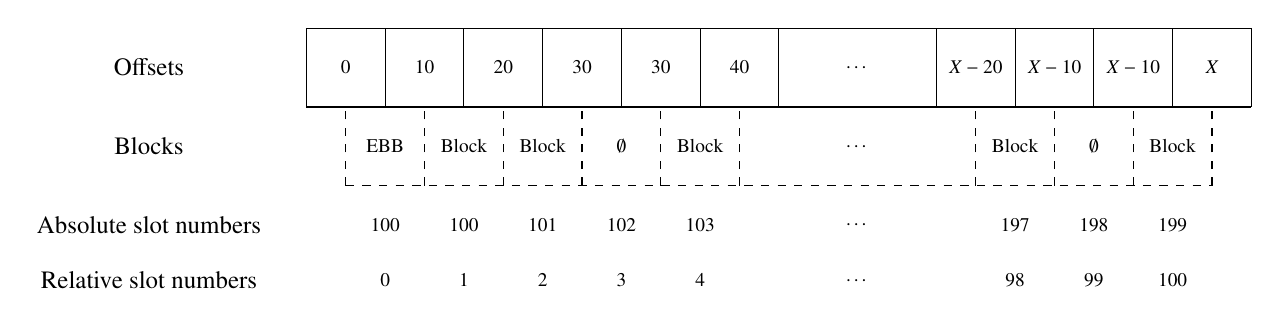
\begin{tikzpicture}
\draw (0, 0)  -- (12, 0);
\draw (0, 1)  -- (12, 1);

\draw ( 0, 0) -- ( 0, 1);
\draw ( 1, 0) -- ( 1, 1);
\draw ( 2, 0) -- ( 2, 1);
\draw ( 3, 0) -- ( 3, 1);
\draw ( 4, 0) -- ( 4, 1);
\draw ( 5, 0) -- ( 5, 1);
\draw ( 6, 0) -- ( 6, 1);
\draw ( 8, 0) -- ( 8, 1);
\draw ( 9, 0) -- ( 9, 1);
\draw (10, 0) -- (10, 1);
\draw (11, 0) -- (11, 1);
\draw (12, 0) -- (12, 1);

\draw (-2.0, 0.5) node {\small Offsets};
\draw ( 0.5, 0.5) node {\scriptsize  0};
\draw ( 1.5, 0.5) node {\scriptsize 10};
\draw ( 2.5, 0.5) node {\scriptsize 20};
\draw ( 3.5, 0.5) node {\scriptsize 30};
\draw ( 4.5, 0.5) node {\scriptsize 30};
\draw ( 5.5, 0.5) node {\scriptsize 40};
\draw ( 7.0, 0.5) node {\scriptsize \ldots};
\draw ( 8.5, 0.5) node {\scriptsize $X - 20$};
\draw ( 9.5, 0.5) node {\scriptsize $X - 10$};
\draw (10.5, 0.5) node {\scriptsize $X - 10$};
\draw (11.5, 0.5) node {\scriptsize $X$};

\draw[dashed] (0.5, -1) -- (11.5, -1);

\draw[dashed] ( 0.5, -1) -- ( 0.5, 0);
\draw[dashed] ( 1.5, -1) -- ( 1.5, 0);
\draw[dashed] ( 2.5, -1) -- ( 2.5, 0);
\draw[dashed] ( 3.5, -1) -- ( 3.5, 0);
\draw[dashed] ( 4.5, -1) -- ( 4.5, 0);
\draw[dashed] ( 5.5, -1) -- ( 5.5, 0);
\draw[dashed] ( 8.5, -1) -- ( 8.5, 0);
\draw[dashed] ( 9.5, -1) -- ( 9.5, 0);
\draw[dashed] (10.5, -1) -- (10.5, 0);
\draw[dashed] (11.5, -1) -- (11.5, 0);

\draw (-2.0, -0.5) node {\small Blocks};
\draw ( 1.0, -0.5) node {\scriptsize EBB};
\draw ( 2.0, -0.5) node {\scriptsize Block};
\draw ( 3.0, -0.5) node {\scriptsize Block};
\draw ( 4.0, -0.5) node {\scriptsize $\emptyset$};
\draw ( 5.0, -0.5) node {\scriptsize Block};
\draw ( 7.0, -0.5) node {\scriptsize \ldots};
\draw ( 9.0, -0.5) node {\scriptsize Block};
\draw (10.0, -0.5) node {\scriptsize $\emptyset$};
\draw (11.0, -0.5) node {\scriptsize Block};

\draw (-2.0, -1.5) node {\small Absolute slot numbers};
\draw ( 1.0, -1.5) node {\scriptsize 100};
\draw ( 2.0, -1.5) node {\scriptsize 100};
\draw ( 3.0, -1.5) node {\scriptsize 101};
\draw ( 4.0, -1.5) node {\scriptsize 102};
\draw ( 5.0, -1.5) node {\scriptsize 103};
\draw ( 7.0, -1.5) node {\scriptsize \ldots};
\draw ( 9.0, -1.5) node {\scriptsize 197};
\draw (10.0, -1.5) node {\scriptsize 198};
\draw (11.0, -1.5) node {\scriptsize 199};

\draw (-2.0, -2.2) node {\small Relative slot numbers};
\draw ( 1.0, -2.2) node {\scriptsize 0};
\draw ( 2.0, -2.2) node {\scriptsize 1};
\draw ( 3.0, -2.2) node {\scriptsize 2};
\draw ( 4.0, -2.2) node {\scriptsize 3};
\draw ( 5.0, -2.2) node {\scriptsize 4};
\draw ( 7.0, -2.2) node {\scriptsize \ldots};
\draw ( 9.0, -2.2) node {\scriptsize 98};
\draw (10.0, -2.2) node {\scriptsize 99};
\draw (11.0, -2.2) node {\scriptsize 100};

\end{tikzpicture}
\end{center}

The version number we mentioned above can be used to migrate indices in the old
format to a newer format, when the need would arise in the future. We do not
include a version number in the secondary index, as both index formats are
tightly coupled, which means that both index files should be migrated together.

One might realise that because the size of a secondary index entry is static,
the primary index could be represented more compactly using a bitmap. This is
indeed the case and the reason for it not being a bitmap is mostly a historical
accident. However, this accident has the upside that migrating to variable-sized
secondary index entries, e.g., serialised using CBOR instead of
\lstinline!Binary! is straightforward.

\paragraph{Lookup}

Having discussed both index formats, we can now finally detail the process of
looking up a block by a point. Given a point with slot $s$ and hash $h$, we need
to go through the following steps to read the corresponding block:

\begin{enumerate}
\item Determine the chunk number $c = \chunkNumber{s}$.
\item Determine the relative slot $\mathit{rs}$ within chunk $c$ corresponding
  to $s$: $\mathit{rs} = \relativeSlot{s}{\mathit{isEBB}}$.

  Note the $\mathit{isEBB}$ argument, which is unknown at this point. Just by
  looking at the slot and the static chunk size, we can tell whether the block
  \emph{could} be an EBB or not: only the very first slot in a chunk (which has
  the same size as a Byron epoch) could correspond to an EBB \emph{or} the
  regular block after it. For all other slots we are certain they cannot
  correspond to an EBB.

  In case the slot $s$ corresponds to the very first slot in the chunk, we will
  have to use the hash $h$ to determine whether the point corresponds to the EBB
  or the regular block in slot $s$.
\item We lookup the offset at $\mathit{rs}$ and the offset after it in the
  primary index of chunk $c$. As discussed, these lookups go through a cache and
  are cheap. We now have the offsets in the secondary index file corresponding
  to the start and end of the secondary index entry we are interested in. If
  both offsets are equal, the slot is empty, and the lookup process terminates.

  In case of a potential EBB, we have to do two such lookups: once for relative
  slot 0 and once for relative slot 1.

\item We read the secondary index entry from the secondary index file. The
  secondary indices are also cached on a per chunk basis. The secondary index
  entry contains the header hash, which we can now compare against $h$. In case
  of a match, we can read the block from the chunk file using the block offset
  contained in the secondary index entry. When the hash does not match, the
  lookup process terminates.

  In case of a potential EBB, the hash comparisons finally tell us whether the
  point corresponds to the EBB or the regular block in slot $s$, or
  \emph{neither} in case both hashes do not match $h$.
\end{enumerate}

\subsection{Recovery}
\label{immutable:implementation:recovery}

Because of the specific requirements of the Immutable DB and the expected write
patterns, we can use a much simpler recovery scheme than traditional database
systems. Only the immutable, append-only part of the chain is stored, which
means that data inconsistencies (e.g., because of a hard shutdown) are most
likely to happen at the end of the chain, i.e., in the last chunk and its
indices. We can simply truncate the chain in such cases. As we maintain some
overlap with the Volatile DB\todo{link}, blocks truncated from the end of the
chain are likely to still be in the Volatile DB, making the recovery process
unnoticeable. If the overlap is not enough and the truncated blocks are not in
the Volatile DB, they can simply be downloaded again.

There are two modes of recovery:
\begin{enumerate}
\item Validate the last chunk: this is the default mode when opening the
  Immutable DB. The last chunk file and its indices are validated. This will
  detect and truncate append operations that did not go through entirely, e.g.,
  a block that was only partially appended to a chunk file, or a block that was
  appended to one or both of the indices, but not to the chunk file.

  When after truncating a chunk file, the chunk file becomes empty, we validate
  the chunk file before it. In the unlikely case that that chunk file has to be
  truncated and ends up empty too, we validate the chunk file before it and so
  on, until we reach a valid block or the database is empty.

\item Validate all chunks: this is the full recovery mode that is triggered by a
  dirty shut down, caused by a missing or corrupted file (e.g., a checksum
  mismatch while reading), or because the node itself was not shut down
  properly.\todo{In the latter case, validating the last would be enough} We
  validate all chunk files and their indices, from oldest to newest. When a
  corrupt or missing block is encountered, we truncate the chain to the last
  valid block before it. Trying to recover from a chain with holes in it would
  be terribly complex, we therefore do not even try it.

\end{enumerate}
In both recovery modes, chunks are validated the same way, which we will shortly
describe. When in full recovery mode, we also check whether the last block in a
chunk is the predecessor of the first block in the next chunk, by comparing the
hashes. This helps sniff out a truncated chunk file that is not the final one,
causing a gap in the chain.

Validating a chunk proceeds as follows:
\begin{itemize}
\item In the common case, the chunk file and the corresponding primary and
  secondary index files will be present and all valid. We optimise for this
  case.\footnote{Unlike in other areas, where we try to maintain that the
  average case is equal to the worst case.}

\item The secondary index contains a CRC32 checksum of each block in the
  corresponding chunk (see \cref{immutable:implementation:indices}), we extract
  these checksums and pass them to the \emph{chunk file parser}.

\item The chunk file parser will try to deserialise all blocks in a chunk file.
  When a block fails to deserialise, it is treated as corrupt and we truncate
  the chain to the last valid block before it. Each raw block is also checked
  against the CRC32 checksum from the secondary index, to detect corruptions
  that are not caught by deserialising, e.g., flipping a bit in a
  \lstinline!Word64!, which can remain a valid, yet corrupt
  \lstinline!Word64!.\footnote{One might think that deserialising the blocks is
  not necessary if the checksums all match. However, the chunk file parser also
  the corresponding secondary index, which is used to validate the on-disk one.
  For this process deserialisation is required.}

  When the CRC32 checksum is not available, because of a missing or partial
  secondary index file, we fall back to the more expensive validation of the
  block based on its cryptographic hashes to detect silent corruption. This type
  of validation is block-dependent and provided in the form of the
  \lstinline!nodeCheckIntegrity! method of the \lstinline!NodeInitStorage!
  class. This validation is implemented by hashing the body of the block and
  comparing it against the body hash stored in the header, and by verifying the
  signature of the header.

  When the CRC32 checksum \emph{is} available, but does not match the one
  computed from the raw block, we also fall back to this validation, as we do
  not know whether the checksum or the block was corrupted (although the latter
  is far more likely).

  The chunk file parser also verifies that the hashes line up within a chunk, to
  detect missing blocks. It does this by comparing the ``previous hash'' of each
  block with the previous block's hash.

  The chunk file parser returns a list of secondary index entries, forming
  together the corresponding secondary index.

\item The chunk file containing the blocks is our source of truth. To check the
  validity of the secondary index, we check whether it matches the secondary
  index returned by the chunk file parser. If there is a mismatch, we overwrite
  the entire secondary index file using the secondary index returned by the
  chunk file parser.

\item We can reconstruct the primary index from the secondary index returned by
  the chunk file parser. When the on-disk primary index is missing or it is not
  equal to the reconstructed one, we (over)write it using the reconstructed one.

\item When truncating the chain, we always make sure that the resulting chain
  ends with a block, i.e., a filled slot, not an empty slot. Even if this means
  going back to the previous chunk.

\end{itemize}

We test the recovery process in our \lstinline!quickcheck-state-machine! tests
of the Immutable DB. In various states of the Immutable DB, we generate one or
more random corruptions for any of the on-disk files: either a simple deletion
of the file, a truncation, or a random bitflip. We verify that after restarting
the Immutable DB, it has recovered to the last valid block before the
truncation.

Additionally, in those same tests, we simulate file-system errors during
operations. For example, while appending a block, we let the second disk write
fail. This is another way of testing whether we can correctly recover from a
write that was aborted half-way through.

\chapter{Volatile Database}
\label{volatile}

The Volatile DB is tasked with storing the blocks that are part of the
\emph{volatile} part of the chain. Do not be misled by its name, the Volatile DB
\emph{should persist} blocks stored to disk. The volatile part of the chain
consists of the last $k$ (the security parameter, see
\cref{consensus:overview:k}) blocks of the chain, which can still be rolled back
when switching to a fork. This means that unlike the Immutable DB, which stores
the immutable prefix of \emph{the} chosen chain, the Volatile DB can store
potentially multiple chains, one of which will be the current chain. It will
also store forks that we have switched away from, or will still switch to, when
they grow longer and become preferable to our current chain. Moreover, the
Volatile DB can contain disconnected blocks, as the block fetch
client\todo{link} might download or receive blocks out of order.

We list the requirements and non-requirements of this component in no particular
order. Note that some of these requirements were defined in response to the
requirements of the Immutable DB (see \cref{immutable}), and vice versa.

\begin{itemize}
\item \textbf{Add-only}: new blocks are always added, never modified.
\item \textbf{Out-of-order}: new blocks can be added in any order, i.e.,
  consecutive blocks on a chain are not necessarily added consecutively. They
  can arrive in any order and can be interspersed with blocks from other chains.
\item \textbf{Garbage-collected}: blocks in the current chain that become older
  than $k$, i.e., there are at least $k$ more recent blocks in the current chain
  after them, are copied from the Volatile DB to the Immutable DB, as they move
  from the volatile to the immutable part of the chain. After copying them to
  the Immutable DB, they can be \emph{garbage collected} from the Volatile DB.

  Blocks that are not part of the chain but are too old to switch to, should
  also be garbage collected.
\item \textbf{Overlap}: by allowing an \emph{overlap} of blocks between the
  Immutable DB and the Volatile DB, i.e., by delaying garbage collection so that
  it does not happen right after copying the block to the Immutable DB, we can
  weaken the durability requirement on the Immutable DB. Blocks truncated from
  the end of the Immutable DB will likely still be in the Volatile DB, and can
  simply be copied again.\todo{done by ChainDB}
\item \textbf{Durability}: similar to the Immutable DB's durability
  \emph{non-requirement}, losing a block because of a crash in the middle or
  right after appending a block is inconsequential. The block can be downloaded
  again.
\item \textbf{Size}: because of garbage collection, there is a bound on the size
  of the Volatile DB in terms of blocks: in the order of $k$, which is 2160 for
  mainnet (we give a more detailed estimate of the size in
  \cref{volatile:implementation:gc}). This makes the size of the Volatile DB
  relatively small, allowing for some information to be kept in memory instead
  of on disk.
\item \textbf{Reading}: the database should be able to return the block or
  header corresponding to the given hash efficiently. Unlike the Immutable DB,
  we do not index by slot numbers, as multiple blocks, from different forks, can
  have the same slot number. Instead, we use header hashes.
\item \textbf{Queries}: it should be possible to query information about blocks.
  For example, we need to be able to efficiently tell which blocks are stored in
  the Volatile DB, or construct a path through the Volatile DB connecting a
  block to another one by chasing its predecessors.\footnote{Note that
  implementing this efficiently using SQL is not straightforward.} Such
  operations should produce consistent results, even while blocks are being
  added and garbage collected concurrently.
\item \textbf{Recoverability}: because of its small size and it being acceptable
  to download missing blocks again, it is not of paramount importance to be able
  to recover as many blocks as possible in case of a corruption.

  However, corrupted blocks should be detected and deleted from the Volatile DB.
\item \textbf{Efficient streaming}: while blocks will be streamed from the
  Volatile DB, this requirement is not as important as it is for the Immutable
  DB. Only a small number of blocks will reside in the Volatile DB, hence fewer
  blocks will be streamed. Most commonly, the block at the tip of the chain will
  be streamed from the Volatile DB (and possibly some of its predecessors). In
  this case, efficiently being able to read a single block will suffice.
\end{itemize}

\section{API}
\label{volatile:api}

Before we describe the implementation of the Volatile DB, we first describe its
functionality. The Volatile DB has the following API:

\begin{lstlisting}
data VolatileDB m blk = VolatileDB {
      closeDB :: m ()

    , putBlock :: blk -> m ()

    , getBlockComponent ::
           forall b.
           BlockComponent blk b
        -> HeaderHash blk
        -> m (Maybe b)

    , garbageCollect :: SlotNo -> m ()

    , getBlockInfo :: STM m (HeaderHash blk -> Maybe (BlockInfo blk))

    , filterByPredecessor :: STM m (ChainHash blk -> Set (HeaderHash blk))

    , getMaxSlotNo :: STM m MaxSlotNo
    }
\end{lstlisting}

The database is parameterised over the block type \lstinline!blk! and the monad
\lstinline!m!, like most of the consensus layer.\todo{mention io-sim}
\todo{TODO} Mention our use of records for components?

The \lstinline!closeDB! operation closes the database, allowing all opened
resources, including open file handles, to be released. This is typically only
used when shutting down the entire system. Calling any other operation on an
already-closed database should result in an exception.

The \lstinline!putBlock! operation adds a block to the Volatile DB. There are no
requirements on this block. This operation is idempotent, as duplicate blocks
are ignored.

The \lstinline!getBlockComponent! operation allows reading one or more
components of the block in the database with the given hash. See
\cref{immutable:api:block-component} for a discussion about block components. As
no block with the given hash might be in the Volatile DB, this operation returns
a \lstinline!Maybe!.

The \lstinline!garbageCollect! operation will try to garbage collect all blocks
with a slot number less than the given one. This will be called after copying a
block with the given slot number to the Immutable DB. Note that the condition is
``less than'', not ``less than or equal to'', even though after a block with
slot $s$ has become immutable, any other blocks produced in the same slot $s$
can never be adopted again and can thus safely be garbage collected. Moreover,
the block we have just copied to the Immutable DB will not even be garbage
collected from the Volatile DB (that will be done after copying its successor
and triggering a garbage collection for the successor's slot number).

The reason for ``less than'' is because of EBBs (\cref{ebbs}). An EBB has the
same slot number as its successor. This means that if an EBB has become
immutable, and we were to garbage collected all blocks with a slot less than or
\emph{equal} to its slot number, we would garbage collect its successor block
too, before having copied it to the Immutable DB.

The next two operations, \lstinline!getBlockInfo! and
\lstinline!filterByPredecessor!, allow querying the Volatile DB. Both operations
are \lstinline!STM!-transactions that return a function. This means that they
can both be called in the same transaction to ensure they produce results that
are consistent w.r.t.\ each other.

The \lstinline!getBlockInfo! operation returns a function to look up the
\lstinline!BlockInfo! corresponding to a block's hash. The \lstinline!BlockInfo!
data type is defined as follows:
\begin{lstlisting}
data BlockInfo blk = BlockInfo {
      biHash         :: !(HeaderHash blk)
    , biSlotNo       :: !SlotNo
    , biBlockNo      :: !BlockNo
    , biPrevHash     :: !(ChainHash blk)
    , biIsEBB        :: !IsEBB
    , biHeaderOffset :: !Word16
    , biHeaderSize   :: !Word16
    }
\end{lstlisting}
This is similar to the information stored in the Immutable DB's on-disk indices,
see \cref{immutable:implementation:indices}. However, in this case, the
information has to be retrieved from an in-memory index, as the function
returned from the \lstinline!STM! transaction is pure.

The \lstinline!filterByPredecessor! operation returns a function to look up the
successors of a given \lstinline!ChainHash!. The \lstinline!ChainHash! data type
is defined as follows:\todo{Explain somewhere else and link?}
\begin{lstlisting}
data ChainHash b =
    GenesisHash
  | BlockHash !(HeaderHash b)
\end{lstlisting}
This extends the header hash type with a case for genesis, which is needed to
look up the blocks that fit onto genesis. As the Volatile DB can store multiple
forks, multiple blocks can have the same predecessor, hence a \emph{set} of
header hashes is returned. This mapping is derived from the ``previous hash''
stored in each block's header. Consequently, the set will only contain the
header hashes of blocks that are currently in the Volatile DB. Hence the choice
for the \lstinline!filterByPredecessor! name instead of the slightly misleading
\lstinline!getSuccessors!. This operation can be used to efficiently construct a
path between two blocks in the Volatile DB. Note that only a single access to
the Volatile DB is need to retrieve the function instead of an access \emph{per
lookup}.

The final operation, \lstinline!getMaxSlotNo!, is also an STM query, returning
the highest slot number stored in the Volatile DB so far. The
\lstinline!MaxSlotNo! data type is defined as follows:
\begin{lstlisting}
data MaxSlotNo =
    NoMaxSlotNo
  | MaxSlotNo !SlotNo
\end{lstlisting}
This is used as an optimisation of fragment filtering in the block fetch
client\todo{link}, look up the \lstinline!filterWithMaxSlotNo! function for more
information.

\section{Implementation}
\label{volatile:implementation}

We will now give a high-level overview of our custom implementation of the
Volatile DB that satisfies the requirements and the API.

\begin{itemize}
\item We append each new block, without any extra information before or after
  it, to a file. When $x$ blocks have been appended to the file, the file is
  closed and a new file is created.

  The smaller $x$, the more files are created.\todo{mention downsides} The
  higher $x$, the longer it will take for a block to be garbage collected, as
  explained in \cref{volatile:implementation:gc}. The default value for $x$ is
  currently \num{1000}.

  For each file, we track the following information:
  \begin{lstlisting}
  data FileInfo blk = FileInfo {
      maxSlotNo :: !MaxSlotNo
    , hashes    :: !(Set (HeaderHash blk))
    }
  \end{lstlisting}
  The \lstinline!maxSlotNo! field caches the highest slot number stored in the
  file. To compute the global \lstinline!MaxSlotNo!, we simply take the maximum
  of these \lstinline!maxSlotNo! fields.

\item We \emph{do not flush} any writes to disk, as discussed in the
  introduction of this chapter. This makes writing a block quite cheap: the
  serialised block is copied to an OS buffer, which is then asynchronously
  flushed in the background.

\item Besides tracking some information per file, we also maintain two in-memory
  indices to implement the \lstinline!getBlockInfo! and
  \lstinline!filterByPredecessor! operations.

  The first index, called the \lstinline!ReverseIndex!\footnote{In a sense, this
  is the reverse of the mapping from file to \lstinline!FileInfo!, hence the
  name \lstinline!ReverseIndex!.} is defined as follows:
  \begin{lstlisting}
  type ReverseIndex blk = Map (HeaderHash blk) (InternalBlockInfo blk)

  data InternalBlockInfo blk = InternalBlockInfo {
        ibiFile        :: !FsPath
      , ibiBlockOffset :: !BlockOffset
      , ibiBlockSize   :: !BlockSize
      , ibiBlockInfo   :: !(BlockInfo blk)
      , ibiNestedCtxt  :: !(SomeSecond (NestedCtxt Header) blk)
      }
  \end{lstlisting}
  In addition to the \lstinline!BlockInfo! that \lstinline!getBlockInfo! should
  return, we also store in which file the block is stored, the offset in the
  file, the size of the block, and the nested context (see
  \cref{serialisation:storage:nested-contents}).

  The second index, called the \lstinline!SuccessorsIndex! is defined as
  follows:
  \begin{lstlisting}
  type SuccessorsIndex blk = Map (ChainHash blk) (Set (HeaderHash blk))
  \end{lstlisting}

  Both indices are updated when new blocks are added and when blocks are removed
  due to garbage collection, see \cref{volatile:implementation:gc}.

  The \lstinline!Map! type used is a strict ordered map from the standard
  \lstinline!containers! package. As for any data that is stored as long-lived
  state, we use strict data types to avoid space leaks. We opt for an ordered
  map, i.e., a sized balanced binary tree, instead of a hashing-based map to
  avoid hash collisions. If an attacker manages to feed us blocks that are
  hashed to the same bucket in the hash map, the performance will deteriorate.
  An ordered map is not vulnerable to this type of attack.

\item Besides the mappings we discussed above, the in-memory state of the
  Volatile DB consists of the path, file handle, and offset into the file to
  which new blocks will be appended. We store this state, a pure data type, in a
  \emph{read-append-write lock}, which we discuss in
  \cref{volatile:implementation:rawlock}.

\item To read a block, header, or any other block component from the Volatile
  DB, we obtain read access to the state (see
  \cref{volatile:implementation:rawlock}) and look up the
  \lstinline!InternalBlockInfo! corresponding to the hash in the
  \lstinline!ReverseIndex!. The found \lstinline!InternalBlockInfo! contains the
  file path, the block offset, and the block size, which is all what is needed
  to read the block. To read the header, we can use the file path, the block
  offset, the nested context (see \cref{serialisation:storage:nested-contents}),
  the header offset, and header size. The other block components can also be
  derived from the \lstinline!InternalBlockInfo!.

\item Note that unlike the Immutable DB, the Volatile DB does not maintain CRC32
  checksums of the stored blocks to detect corruption. Instead, after reading a
  block from the Volatile DB and before copying it to the Immutable DB, we
  validate the block using the \lstinline!nodeCheckIntegrity! method, as
  described in \cref{immutable:implementation:recovery}.

\end{itemize}

\subsection{Garbage collection}
\label{volatile:implementation:gc}

\todo{TODO} Sync with \cref{chaindb:gc}.

As mentioned above, when a garbage collection for slot $s$ is triggered, all
blocks with a slot less than $s$ should be removed from the Volatile DB.

For simplicity and following our robust append-only approach, we do not modify
files in-place during garbage collection. Either all the blocks in a file have a
slot number less than $s$ and it can be deleted atomically, or at least one
block has a slot number greater or equal to $s$ and we do \emph{not} delete the
file. Checking whether a file can be garbage collected is simple and happens in
constant time: the \lstinline!maxSlotNo! field of \lstinline!FileInfo! is
compared against $s$.

The default for blocks per file is currently \num{1000}. Let us now calculate
what the effect of this number is on garbage collection. We will call blocks
that with a slot older than $s$ \emph{garbage}. Garbage blocks that can be
deleted because they are in a file only containing garbage are \emph{collected
garbage}. Garbage blocks that cannot yet be deleted because there is a
non-garbage block in the same file are \emph{uncollected garbage}.

The lower the number of blocks per file, the fewer uncollected garbage there
will be, and vice versa. In the extreme case, a single block is stored per file,
resulting in no uncollected garbage, i.e., a garbage collection rate of 100\%.
The downside is that for each new block to add, a new file will have to be
created, which is less efficient than appending to an already open file. It will
also result in lots of tiny files.

The other extreme is to have no bound on the number of blocks per file, which
will result in one single file containing all blocks. This means no garbage will
ever be collected, i.e., a garbage collection rate of 0\%, which is of course
not acceptable.

During normal operation, roughly one block will be added every 20
seconds.\footnote{When using the PBFT consensus protocol (\cref{bft}), exactly
one block will be produced every 20 seconds. However, when using the Praos
consensus protocol (\cref{praos}), on average there will be one block every 20
seconds, but it is natural to have a fork now and then, leading to one or more
extra blocks. For the purposes of this calculation, the difference is
negligible.} The security parameter $k$ used for mainnet is \num{2160}. This
mean that if a linear chain of \num{2161} blocks has been added, the oldest
block has become immutable and can be copied to the Immutable DB, after which it
can be garbage collected. If we assume no delay between copying and garbage
collection, it will take $\num{1000} + \num{2160} = \num{3160}$ blocks before
the first file containing \num{1000} blocks will be garbage collected.

This means that in the above scenario, starting from a Volatile DB containing
$k$ blocks, after every $\mathsf{blocksPerFile}$ new blocks and thus
corresponding garbage collections, $\mathsf{blocksPerFile}$ blocks will be
garbage collected.\todo{expand calculation}

In practice we allow for overlap by delaying the garbage collection, which has
an impact on the effective size of the Volatile DB, which we discuss in
\todo{link ChainDB}.

\subsection{Read-Append-Write lock}
\label{volatile:implementation:rawlock}

We use a \emph{read-append-write} lock to store the state of the Volatile DB.
This is an extension of the more common read-write lock. A RAW lock allows
multiple concurrent readers, at most one appender, which is allowed to run
concurrently with the readers, and at most one writer, which has exclusive
access to the lock.

The \lstinline!getBlockComponent! operation corresponds to \emph{reading}, the
\lstinline!putBlock! operation to \emph{appending}, and the
\lstinline!garbageCollect! operation to \emph{writing}. Adding a new block can
safely happen at the same time as blocks are being read. The new block will be
appended to the current file or a new file will be started. This does not affect
any concurrent reads of other blocks in the Volatile DB. At most one block can
be added at a time, as blocks are appended one-by-one to the current file. To
garbage collect the Volatile DB, we must obtain an exclusive lock on the state,
as we might be deleting a file while trying to read from it at the same time.
During garbage collection, we ignore the current file and will thus never try to
delete it. This means that, strictly speaking, it would be possible to safely
append blocks and garbage collect blocks concurrently. However, for simplicity
(how should the concurrent changes to the indices be resolved?), we did not
pursue this.

As mentioned in \cref{volatile:implementation:gc}, it is often the case that no
files can be garbage collected. As a (premature) optimisation, we first check
(which is cheap) whether any files can be garbage collected before trying to
obtain the corresponding, more expensive lock on the state.

\subsection{Recovery}
\label{volatile:implementation:recovery}

Whenever a file-system operation fails, or a file is missing or corrupted, we
shut down the Volatile DB and consequently the whole system. When this happens,
either the system's file system is no longer reliable (e.g., disk corruption),
manual intervention (e.g., disk is full) is required, or there is a bug in the
system. In all cases, there is no point in trying to continue operating. We shut
down the system and flag the shutdown as \emph{dirty}, triggering a full
validation on the next start-up.

When opening the Volatile DB, the previous in-memory state, including the
indices, is reconstructed based on the on-disk files. The block in each file are
read and deserialised. There are two validation modes: a standard validation and
a full validation. The difference between the two is that during a full
validation, the integrity of each block is verified to detect silent corruption
using the \lstinline!nodeCheckIntegrity! method, as described in
\cref{immutable:implementation:recovery}.

When a block fails to deserialise or it is detected as a corrupt block when the
full validation mode is enabled, the file is truncated to the last valid block
before it. As mentioned at the start of this chapter, it is not crucial to
recover every single block. Therefore, we do not try to deserialise the blocks
after a corrupt one.

\chapter{Ledger Database}
\label{ledgerdb}

The Ledger DB is responsible for the following tasks:

\begin{enumerate}
\item \textbf{Maintaining the ledger state at the tip}: Maintaining the ledger
  state corresponding to the current tip in memory. When we try to extend our
  chain with a new block fitting onto our tip, the block must first be validated
  using the right ledger state, i.e., the ledger state corresponding to the tip.
  The current ledger state is needed for various other purposes.

\item \textbf{Maintaining the past $k$ ledger states}: As discussed in
  \cref{consensus:overview:k}, we might roll back up to $k$ blocks when
  switching to a more preferable fork. Consider the example below:
  %
  \begin{center}
  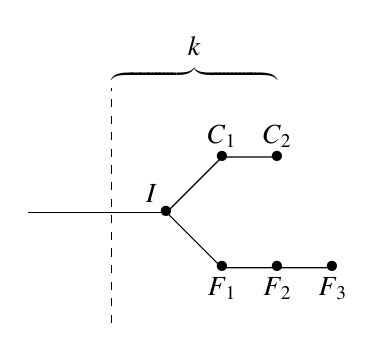
\begin{tikzpicture}
  \draw (0, 0) -- (50pt, 0) coordinate (I);
  \draw (I) -- ++(20pt,  20pt) coordinate (C1) -- ++(20pt, 0) coordinate (C2);
  \draw (I) -- ++(20pt, -20pt) coordinate (F1) -- ++(20pt, 0) coordinate (F2) -- ++(20pt, 0) coordinate (F3);
  \node at (I)  {$\bullet$};
  \node at (C1) {$\bullet$};
  \node at (C2) {$\bullet$};
  \node at (F1) {$\bullet$};
  \node at (F2) {$\bullet$};
  \node at (F3) {$\bullet$};
  \node at (I) [above left] {$I$};
  \node at (C1) [above] {$C_1$};
  \node at (C2) [above] {$C_2$};
  \node at (F1) [below] {$F_1$};
  \node at (F2) [below] {$F_2$};
  \node at (F3) [below] {$F_3$};
  \draw (60pt, 50pt) node {$\overbrace{\hspace{60pt}}$};
  \draw (60pt, 60pt) node[fill=white] {$k$};
  \draw [dashed] (30pt, -40pt) -- (30pt, 45pt);
  \end{tikzpicture}
  \end{center}
  %
  Our current chain's tip is $C_2$, but the fork containing blocks $F_1$, $F_2$,
  and $F_3$ is more preferable. We roll back our chain to the intersection point
  of the two chains, $I$, which must be not more than $k$ blocks back from our
  current tip. Next, we must validate block $F_1$ using the ledger state at
  block $I$, after which we can validate $F_2$ using the resulting ledger state,
  and so on.

  This means that we need access to all ledger states of the past $k$ blocks,
  i.e., the ledger states corresponding to the volatile part of the current
  chain.\footnote{Applying a block to a ledger state is not an invertible
  operation, so it is not possible to simply ``unapply'' $C_1$ and $C_2$ to
  obtain $I$.}

  Access to the last $k$ ledger states is not only needed for validating candidate
  chains, but also by the:
  \begin{itemize}
  \item \textbf{Local state query server}: To query any of the past $k$ ledger
    states (\cref{servers:lsq}).
  \item \textbf{Chain sync client}: To validate headers of a chain that
    intersects with any of the past $k$ blocks
    (\cref{chainsyncclient:validation}).
  \end{itemize}

\item \textbf{Storing on disk}: To obtain a ledger state for the current tip of
  the chain, one has to apply \emph{all blocks in the chain} one-by-one to the
  initial ledger state. When starting up the system with an on-disk chain
  containing millions of blocks, all of them would have to be read from disk and
  applied. This process can take tens of minutes, depending on the storage and
  CPU speed, and is thus too costly to perform on each startup.

  For this reason, a recent snapshot of the ledger state should be periodically
  written to disk. Upon the next startup, that snapshot can be read and used to
  restore the current ledger state, as well as the past $k$ ledger states.
\end{enumerate}

Note that whenever we say ``ledger state'', we mean the
\lstinline!ExtLedgerState blk! type described in \cref{storage:extledgerstate}.

The above duties are divided across the following modules:

\begin{itemize}
\item \lstinline!LedgerDB.InMemory!: this module defines a pure data structure,
  named \lstinline!LedgerDB!, to represent the last $k$ ledger states in memory.
  Operations to validate and append blocks, to switch to forks, to look up
  ledger states, \ldots{} are provided.
\item \lstinline!LedgerDB.OnDisk!: this module contains the functionality to
  write a snapshot of the \lstinline!LedgerDB! to disk and how to restore a
  \lstinline!LedgerDB! from a snapshot.
\item \lstinline!LedgerDB.DiskPolicy!: this module contains the policy that
  determines when a snapshot of the \lstinline!LedgerDB! is written to disk.
\item \lstinline!ChainDB.Impl.LgrDB!: this module is part of the Chain DB, and
  is responsible for maintaining the pure \lstinline!LedgerDB! in a
  \lstinline!StrictTVar!.
\end{itemize}

We will now discuss the modules listed above.

\section{In-memory representation}
\label{ledgerdb:in-memory}

The \lstinline!LedgerDB!, capable of represent the last $k$ ledger states, is an
instantiation of the \lstinline!AnchoredSeq! data type. This data type is
implemented using the \emph{finger tree} data structure~\cite{fingertrees} and
has the following time complexities:

\begin{itemize}
\item Appending a new ledger state to the end in constant time.
\item Rolling back to a previous ledger state in logarithmic time.
\item Looking up a past ledger state by its point in logarithmic time.
\end{itemize}

One can think of a \lstinline!AnchoredSeq! as a \lstinline!Seq! from
\lstinline!Data.Sequence! with a custom \emph{finger tree measure}, allowing for
efficient lookups by point, combined with an \emph{anchor}. When fully
\emph{saturated}, the sequence will contain $k$ ledger states. In case of a
complete rollback of all $k$ blocks and thus ledger states, the sequence will
become empty. A ledger state is still needed, i.e., one corresponding to the
most recent immutable block that cannot be rolled back. The ledger state at the
anchor plays this role.

When a new ledger state is appended to a fully saturated \lstinline!LedgerDB!,
the ledger state at the anchor is dropped and the oldest element in the sequence
becomes the new anchor, as it has become immutable. This maintains the invariant
that only the last $k$ ledger states are stored, \emph{excluding} the ledger
state at the anchor. This means that in practice, $k + 1$ ledger states will be
kept in memory. When fewer the \lstinline!LedgerDB! contains fewer than $k$
elements, new ones are appended without shifting the anchor until it is
saturated.

\todo{TODO} figure?

The \lstinline!LedgerDB! is parameterised over the ledger state $l$.
Conveniently, the \lstinline!LedgerDB! can implement the same abstract interface
(described in \cref{ledger:api}) that the ledger state itself implements. I.e.,
the \lstinline!GetTip!, \lstinline!IsLedger!, and \lstinline!ApplyBlock!
classes. This means that in most places, wherever a ledger state can be used, it
is also possible to wrap it in a \lstinline!LedgerDB!, causing it to
automatically maintain a history of the last $k$ ledger states.

\todo{TODO} discuss \lstinline!Ap! and \lstinline!applyBlock!? These are
actually orthogonal to \lstinline!LedgerDB! and should be separated.


\paragraph{Memory usage}

The ledger state is a big data structure that contains, amongst other things,
the entire UTxO. Recent measurements\footnote{Using the ledger state at the
block with slot number \num{16976076} and hash \lstinline!af0e6cb8ead39a86!.}
show that the heap size of an Allegra ledger state is around \num{361}~MB.
Fortunately, storing $k = \num{2160}$ ledger states in memory does \emph{not}
require $\num{2160} * \num{361}~\textrm{MB} = \num{779760}~\textrm{MB} =
\num{761}~\textrm{GB}$. The ledger state is defined using standard Haskell data
structures, e.g., \lstinline!Data.Map.Strict!, which are \emph{persistent} data
structures. This means that when we update a ledger state by applying a block to
it, we only need extra memory for the new and the modified data. The majority of
the data will stay the same and will be \emph{shared} with the previous ledger
state.

The memory required for storing the last $k$ ledger state is thus proportional
to: the size of the oldest in-memory ledger state \emph{and} the changes caused
by the last $k$ blocks, e.g., the number of transactions in those blocks.
Compared to the \num{361}~MB required for a single ledger state, keeping the
last $k$ ledger states in memory requires only \num{375}~MB in total. This is
only \num{14}~MB or 3.8\% more memory. Which is a very small cost.

\paragraph{Past design}

In the past, before measuring this cost, we did not keep all $k$ past ledger
states because of an ungrounded fear for the extra memory usage. The
\lstinline!LedgerDB! data structure had a \lstinline!snapEvery! parameter,
ranging from 1 to $k$, indicating that a snapshot, i.e., a ledger state, should
be kept every \lstinline!snapEvery! ledger states or blocks. In practice, a
value of 100 was used for this parameter, resulting in 21--22 ledger states in
memory.

The representation was much more complex, to account for these missing ledger
states. More importantly, accessing a past ledger state or rewinding the
\lstinline!LedgerDB! to a past ledger state had a very different cost model. As
the requested ledger state might not be in memory, it would have to be
\emph{reconstructed} by reapplying blocks to an older ledger state.

Consider the example below using \lstinline!snapEvery! = 3. $L_i$ indicate
ledger states and $\emptyset_i$ indicate skipped ledger states. $L_0$ corresponds to the
most recent ledger state, at the tip of the chain.
%
\begin{center}
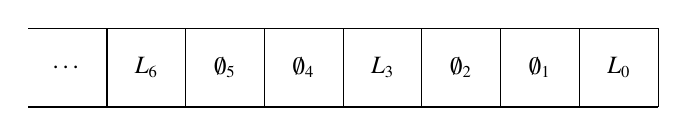
\begin{tikzpicture}
\draw (0, 0) -- (8, 0);
\draw (0, 1) -- (8, 1);

\draw (1, 0) -- (1, 1);
\draw (2, 0) -- (2, 1);
\draw (3, 0) -- (3, 1);
\draw (4, 0) -- (4, 1);
\draw (5, 0) -- (5, 1);
\draw (6, 0) -- (6, 1);
\draw (7, 0) -- (7, 1);
\draw (8, 0) -- (8, 1);

\draw (0.5, 0.5) node {\small \ldots};
\draw (1.5, 0.5) node {\small $L_6$};
\draw (2.5, 0.5) node {\small $\emptyset_5$};
\draw (3.5, 0.5) node {\small $\emptyset_4$};
\draw (4.5, 0.5) node {\small $L_3$};
\draw (5.5, 0.5) node {\small $\emptyset_2$};
\draw (6.5, 0.5) node {\small $\emptyset_1$};
\draw (7.5, 0.5) node {\small $L_0$};

\end{tikzpicture}
\end{center}
%
When we need access to the ledger state at position $3$, we are in luck and can
use the available $L_3$. However, when we need access to the skipped ledger
state at position $1$, we have to do the following: we look for the most recent
ledger state before $\emptyset_1$, i.e., $L_3$. Next, we need to reapply blocks $B_2$
and $B_1$ to it, which means we have to read those from disk, deserialise them,
and apply them again.

This means that accessing a past ledger state is not a pure operation and might
require disk access and extra computation. Consequently, switching to a fork
might require reading and revalidating blocks that remain part of the chain, in
addition to the new blocks.

As mentioned at the start of this chapter, the chain sync client also needs
access to past ledger view (\cref{consensus:class:ledgerview}), which it can
obtain from past ledger states. A malicious peer might try to exploit it and
create a chain that intersects with our chain right \emph{before} an in-memory
ledger state snapshot. In the worst case, we have to read and reapply
\lstinline!snapEvery! - 1 = 99 blocks. This is not acceptable as the costs are
asymmetric and in the advantage of the attacker, i.e., creating and serving such
a header is much cheaper than reconstructing the required snapshot. At the time,
we solved this by requiring ledger states to store snapshots of past ledger
views. The right past ledger view could then be obtained from the current ledger
state, which was always available in memory. However, storing snapshots of
ledger views within a single ledger state is more complex, as we are in fact
storing snapshots \emph{within} snapshots. The switch to keep all $k$ past
ledger states significantly simplified the code and sped up the look-ups.

\paragraph{Future design}

It is important to note that in the future, this design will have to change
again. The UTxO and, consequently, the ledger state are expected to grow in size
organically. This growth will be accelerated by new features added to the
ledger, e.g., smart contracts. At some point, the ledger state will be so large
that keeping it in its entirety in memory will no longer be feasible. Moreover,
the cost of generating enough transactions to grow the current UTxO beyond the
expected memory limit might be within reach for some attackers. Such an attack
might cause a part of the network to be shut down because the nodes in question
are no longer able to load the ledger state in memory without running against
the memory limit.

For these reasons, we plan to revise our design in the future, and start storing
parts of the ledger state on disk again.

\section{On-disk}
\label{ledgerdb:on-disk}

The \lstinline!LedgerDB.OnDisk! module provides functions to write a ledger
state to disk and read a ledger state from disk. The \lstinline!EncodeDisk! and
\lstinline!DecodeDisk! classes from \cref{serialisation:storage} are used to
(de)serialise the ledger state to or from CBOR. Because of its large size, we
read and deserialise the snapshot incrementally.

\todo{TODO} which ledger state to take a snapshot from is determined by the
Chain DB. I.e., the background thread that copies blocks from the Volatile DB to
the Immutable DB will call the \lstinline!onDiskShouldTakeSnapshot! function,
and if it returns \lstinline!True!, a snapshot will be taken. \todo{TODO}
double-check whether we're actually taking a snapshot of the right ledger state.

\subsection{Disk policy}
\label{ledgerdb:on-disk:disk-policy}

The disk policy determines how many snapshots should be stored on disk and when
a new snapshot of the ledger state should be written to disk.

\todo{TODO} worth discussing? We would just be duplicating the existing
documentation.

\subsection{Initialisation}
\label{ledgerdb:on-disk:initialisation}

During initialisation, the goal is to construct an initial \lstinline!LedgerDB!
that is empty except for the ledger state at the anchor, which has to correspond
to the immutable tip, i.e., the block at the tip of the Immutable DB
(\cref{immutable}).

Ideally, we can construct the initial \lstinline!LedgerDB! from a snapshot of
the ledger state that we wrote to disk. Remember that updating a ledger state
with a block is not invertible: we can apply a block to a ledger state, but we
cannot ``unapply'' a block to a ledger state. This means the snapshot has to be
at least as old as the anchor. A snapshot matching the anchor can be used as is.
A snapshot older than the anchor can be used after reapplying the necessary
blocks. A snapshot newer than the anchor can \emph{not} be used, as we cannot
unapply blocks to get the ledger state corresponding to the anchor. This is the
reason why we only take snapshots of an immutable ledger state, i.e., of the
anchor of the \lstinline!LedgerDB! (or older).

Constructing the initial \lstinline!LedgerDB! proceeds as follows:
\begin{enumerate}
\item If any on-disk snapshots are available, we try them from new to old. The
  newer the snapshot, the fewer blocks will need to be reapplied.
\item We deserialise the snapshot. If this fails, we try the next one.
\item If the snapshot is of the ledger state corresponding to the immutable tip,
  we can use the snapshot for the anchor of the \lstinline!LedgerDB! and are
  done.
\item If the snapshot is newer than the immutable tip, we cannot use it and try
  the next one. This situation can arise not because we took a snapshot of a
  ledger state newer than the immutable tip, but because the Immutable DB was
  truncated.
\item If the snapshot is older than the immutable tip, we will have to reapply
  the blocks after the snapshot to obtain the ledger state at the immutable tip.
  If there is no (more) snapshot to try, we will have to reapply \emph{all
  blocks} starting from the beginning of the chain to obtain the ledger state at
  the immutable tip, i.e., the entire immutable chain. The blocks to reapply are
  streamed from the Immutable DB, using an iterator
  (\cref{immutable:api:iterators}).

  Note that we can \emph{reapply} these blocks, which is quicker than applying
  them (see \cref{ledgerdb:lgrdb}), as the existence of a snapshot newer than
  these blocks proves\footnote{Unless the on-disk database has been tampered
  with, but this is not an attack we intend to protect against, as this would
  mean the machine has already been compromised.} that they have been
  successfully applied in the past.
\end{enumerate}
%
Reading and applying blocks is costly. Typically, very few blocks need to be
reapplied in practice. However, there is one exception: when the serialisation
format of the ledger state changes, all snapshots (written using the old
serialisation format) will fail to deserialise, and all blocks starting from
genesis will have to be reapplied. To mitigate this, the ledger state decoder is
typically written in a backwards-compatible way, i.e., it accepts both the old
and new serialisation format.

\section{Maintained by the Chain DB}
\label{ledgerdb:lgrdb}

\todo{TODO} move to Chain DB chapter?

The \lstinline!LedgerDB! is a pure data structure. The Chain DB (see
\cref{chaindb}) maintains the current \lstinline!LedgerDB! in a
\lstinline!StrictTVar!. The most recent element in the \lstinline!LedgerDB! is
the current ledger state. Because it is stored in a \lstinline!StrictTVar!, the
current ledger state can be read and updated in the same \lstinline!STM!
transaction as the current chain, which is also stored in a
\lstinline!StrictTVar!.

The \lstinline!ChainDB.Impl.LgrDB!\footnote{In the past, we had similar modules
for the \lstinline!VolatileDB! and \lstinline!ImmutableDB!, i.e.,
\lstinline!VolDB! and \lstinline!ImmDB!. The former were agnostic of the
\lstinline!blk! type and the latter instantiated the former with the
\lstinline!blk! type. However, in hindsight, unifying the two proved to be
simpler and was thus done. The reason why a separate \lstinline!LgrDB! still
exists is mainly because it needs to wrap the pure \lstinline!LedgerDB! in a
\lstinline!StrictTVar!.} is responsible for maintaining the current ledger
state. Besides this responsibility, it also integrates the Ledger DB with other
parts of the Chain DB.

Moreover, it remembers which blocks have been successfully applied in the past.
When such a block needs to be validated again, e.g., because we switch again to
the same fork containing the block, we can \emph{reapply} the block instead of
\emph{applying} it (see \cref{ledger:api:ApplyBlock}). Because the block has
been successfully applied in the past, we know the block is valid, which means
we can skip some of the more expensive checks, e.g., checking the hashes,
speeding up the process of validating the block. Note that a block can only be
applied to a single ledger state, i.e., the ledger state corresponding to the
predecessor of the block. Consequently, it suffices to remember whether a block
was valid or not, there is no need to remember with respect to which ledger
state it was valid.

To remember which blocks have been successfully applied in the past, we store
the points of the respective blocks in a set. Before validating a block, we look
up its point in the set, when present, we can reapply the block instead of
applying it. To stop this set from growing without bound, we garbage collect it
the same way the Volatile DB is garbage collected, see \cref{chaindb:gc}. When a
block has a slot older than the slot number of the most recent immutable block,
either the block is already immutable or it is part of a fork that we will never
consider again, as it forks off before the immutable block.\todo{slot number vs
  block number} The block in question will never have to be validated again, and
so it is not necessary to remember whether we have already applied it or not.

\newcommand{\chainle}{\ensuremath{\mathrel{\sqsubseteq}}}
\newcommand{\chainlt}{\ensuremath{\mathrel{\sqsubset}}}
\newcommand{\chainnotlt}{\ensuremath{\mathrel{\nsqsubset}}}
\newcommand{\wehave}{.\;}
\newcommand{\suchthat}{.\;}
\newcommand{\app}{\ensuremath{\mathrel{\triangleright}}}
\newcommand{\length}[1]{\ensuremath{\mathrm{length} \; #1}}
\newcommand{\ifthen}[2]{\ensuremath{\mathrm{if} \quad #1 \quad \mathrm{then} \quad #2}}
\renewcommand{\iff}{\ensuremath{\qquad\mathrm{iff}\qquad}}
\newcommand{\candidates}[2]{\ensuremath{\mathsf{candidates}_#1(#2)}}
\newcommand{\blockNo}[1]{\ensuremath{\mathtt{blockNo}(#1)}}
\newcommand{\selectviewle}{\ensuremath{\precsim}}

\chapter{Chain Selection}
\label{chainsel}

Chain selection is one of the central responsibilities of the chain database
(\cref{chaindb}). It of course depends on chain selection as it is defined  by
the consensus protocol (\cref{consensus:class:chainsel}), but needs to  take
care of a lot of operational concerns. In this chapter we will take a closer
look at the implementation of chain selection in the chain database, and state
some properties and sketch some proofs to motivate it.

\section{Comparing anchored fragments}
\label{chainsel:fragments}

\subsection{Introduction}

Recall from \cref{consensus:overview:chainsel} that while in the literature
chain selection is defined in terms of comparisons between entire chains, we
instead opted to model it in terms of a comparison between the \emph{headers} at
the tip of those chains (or rather, a \emph{view} on those headers defined by
the specific consensus protocol).

We saw in \cref{storage:inmemory} (specifically, \cref{storage:fragments}) that
the consensus layer stores chain fragments in memory (the most recent headers on
a chain), both for the node's own current chain as well as for upstream nodes
(which we refer to as ``candidate chains''). Defining chain selection in terms
of fragments is straight-forward when those fragments are non-empty: we simply
take the most recent header, extract the view required by the consensus protocol
(\cref{BlockSupportsProtocol}), and then use the consensus protocol's chain
selection interface to compare them. The question is, however, how to compare
two fragments when one (or both) of them is \emph{empty}. This problem is more
subtle than it might seem at first sight, and requires careful consideration.

We mentioned in \cref{consensus:overview:chainsel} that consensus imposes a
fundamental assumption that the strict extension of a chain is always (strictly)
preferred over that chain (\cref{prefer-extension}), and that consequently we
\emph{always} prefer a non-empty chain over an empty one (and conversely we
\emph{never} prefer an empty chain over a non-empty one). However, chain
fragments are mere proxies for their chains, and the fragment might be empty
even if the chain is not. This means that in principle it's possible we do not
prefer a non-empty fragment over an empty one, or indeed prefer an empty
fragment over a non-empty one. However, when a fragment is empty, we cannot rely
on the consensus protocol's chain selection because we have no header to give
it.

Let's consider under which conditions these fragments might be empty:

\begin{description}
\item[Our fragment]
Our own fragment is a path through the volatile database, anchored at the tip of
the immutable database (\cref{storage:fragments}). Under normal circumstances,
it will be empty only if our \emph{chain} is empty; we will refer to such empty
fragments as \emph{genuinely empty}.\footnote{We can distinguish between an empty
fragment of a non-empty chain and a (necessarily) empty fragment of an empty
chain by looking at the anchor point: if it is the genesis point, the chain must
be empty.} However, our fragment can also be empty even when our chain is not,
if due to data loss the volatile database is empty (or contains no blocks that
fit onto the tip of the immutable database).

\item[Candidate fragment]
A \emph{genuinely} empty candidate fragment, representing an empty candidate
chain, is never preferred over our chain. Unfortunately, however, the candidate
fragment as maintained by the chain sync client (\cref{chainsyncclient}) can
essentially be empty at any point due to the way that a switch-to-fork is
implemented in terms of rollback followed by roll forward: after a maximum
rollback (and before the roll forward), the candidate fragment is empty.
\end{description}

\subsection{Precondition}
\label{chainsel:fragments:precondition}

Since neither of these circumstances can be avoided, we must therefore impose a
precondition for chain selection between chain fragments to be definable:

\begin{definition}[Precondition for comparing chain fragments]
The two fragments must either both be non-empty, or they must intersect.
\end{definition}

In this chapter, we establish this precondition in two different ways:

\begin{enumerate}
\item When we construct candidates chains (potential chains that we may wish
to replace our own chain with), those candidate chains must intersect with
our own chain within $k$ blocks from its tip; after all, if that is not the
case, we would induce a roll back of more than $k$ blocks
(\cref{consensus:overview:k}).

\item When we compare fragments to each other, we only compare fragments from a
set of fragments that are all anchored at the same point (i.e., the anchor of
all fragments in the set is the same, though it might be different from the
anchor of our current fragment). Since they are all anchored at the same point,
they trivially all intersect with each other.
\end{enumerate}

There is one more use of fragment selection, which is rather more subtle;
we will come back to this in \cref{chainsyncclient:plausiblecandidates}.

\todo{TODO} TODO: Throughout we are talking about \emph{anchored} fragments
here. We should make sure that we discuss those somewhere.

\subsection{Definition}
\label{chainsel:fragments:definition}

We will now show that this precondition suffices to compare two fragments,
whether or not they are empty; we'll consider each case in turn.

\begin{description}

\item[Both fragments empty]
Since the two fragments must intersect, that intersection point can only
be the two anchor points, which must therefore be equal. This means that
two fragments represent the same chain: neither fragment is preferred
over the other.

\item[First fragment non-empty, second fragment empty]
Since the two fragments must intersect, that intersection can only be the
anchor of the second fragment, which can lie anywhere on the first fragment.

\begin{itemize}
\item If it lies at the \emph{tip} of the first fragment, the two fragments represent the
same chain, and neither is preferred over the other.
\item If it lies \emph{before} the tip of first fragment, the first fragment is
a strict extension of the second, and is therefore is preferred over the
second.
\end{itemize}

\item[First fragment empty, second fragment non-empty]
This case is entirely symmetric to the previous; if the intersection is the
tip of the second fragment, the fragments represent the same chain. Otherwise,
the second fragment is a strict extension of the first, and is therefore
preferred.

\item[Both fragments non-empty]
In this case, we can simply use the consensus protocol chain selection API
to compare the two most recent headers on both fragments.

\end{description}

Note that this relies critically on the ``prefer extension'' rule
(\cref{prefer-extension}).

\section{Preliminaries}
\label{chainsel:spec}

Recall from \cref{storage:components} that the immutable database stores a
linear chain, terminating in the \emph{tip} $I$ of the immutable database. The
volatile database stores a (possibly fragmented) tree of extensions to that
chain:
%
\begin{center}
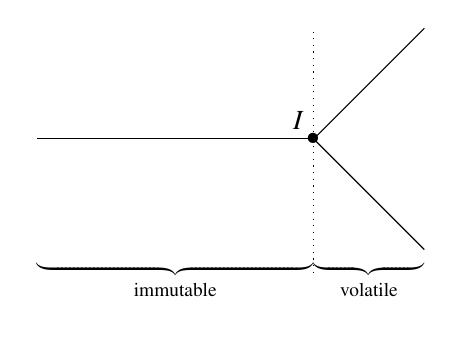
\begin{tikzpicture}
\draw (0,0) -- (100pt, 0) coordinate (immtip) node{$\bullet$} node[above left] {$I$};
\draw (immtip) -- ++(40pt,  40pt);
\draw (immtip) -- ++(40pt, -40pt);
\draw [dotted] (immtip) -- ++(0, 40pt);
\draw [dotted] (immtip) -- ++(0, -50pt);
\node at (50pt, -40pt) [below] {$\underbrace{\hspace{100pt}}_\textrm{immutable}$};
\node at (120pt, -40pt) [below] {$\underbrace{\hspace{40pt}}_\textrm{volatile}$};
\end{tikzpicture}
\end{center}
%
The node's \emph{current chain} is stored in memory as a chain fragment through
the volatile database, anchored at $I$.  When we start up the node, the chain
database must find the best possible path through the volatile database and
adopt that as our current fragment; every time a new block is added to the
volatile database, we have to recompute the new best possible path. In other
words, we maintain the following invariant:

\begin{definition}[Current chain invariant]
\label{current-chain-invariant}
The current chain is the best possible path through the volatile DB.
\end{definition}

``Best'' of course is according to the chain selection rule defined by the
consensus protocol (\cref{consensus:class:chainsel}). In this section we
describe how the chain database establishes and preserves this invariant.

\subsection{Notation}

So far we have been relatively informal in our description of chain selection,
but in order to precisely describe the algorithm and state some of its
properties, we have to introduce some notation.

\begin{definition}[Chain selection]
We will model chain selection as a transitive binary relation (\chainlt) between
valid chains (it is undefined for invalid chains), and let $C \chainle C'$ if
and only if $C \chainlt C'$ or $C = C'$. It follows that (\chainle) is a partial
order (reflexive, antisymmetric, and transitive).
\end{definition}

For example, the simple ``prefer longest chain'' chain selection rule could be
given as
%
\begin{equation*}
\tag{longest chain rule}
C \chainlt C'  \iff  \length{C} < \length{C'}
\end{equation*}

In general of course the exact rule depends on the choice of consensus protocol.
\Cref{prefer-extension} (\cref{consensus:overview:chainsel}) can now be
rephrased as
%
\begin{equation}
\label{eq:prefer-extension}
\forall C, B \wehave C \chainlt (C \app B)
\end{equation}

We will not be comparing whole chains, but rather chain fragments
(we will leave the anchor of fragments implicit):
%
\begin{definition}[Fragment selection]
We lift $\chainlt$ to chain fragments in the manner described in
\cref{chainsel:fragments}; this means that $\chainlt$ is undefined for two
fragments if they do not intersect (\cref{chainsel:fragments:precondition}).
\end{definition}

We also lift $\chainle$ to \emph{sets} of fragments, intuitively indicating that
a particular fragment is the ``best choice'' out of a set $\mathcal{S}$ of
candidate fragments:
%
\begin{definition}[Optimal candidate]
\begin{equation*}
\mathcal{S} \chainle F  \iff   \nexists F' \in \mathcal{S} \suchthat F \chainlt F'
\end{equation*}
(in other words, if additionally $F \in \mathcal{S}$, then $F$ is a maximal
element of $C$). This inherits all the preconditions of $\chainle$ on chains and
fragments.
\end{definition}

Finally, we will introduce some notation for \emph{computing} candidate
fragments:\footnote{In order to compute these candidates efficiently, the
volatile database must support a ``forward chain index'', able to efficiently
answer the question ``which blocks succeed this one?''.}

\begin{definition}[Construct set of candidates]
Given some set of blocks $V$, and some anchor $A$ (with $A$ either a block or
the genesis point), $$\candidates{A}{V}$$ is the set of chain fragments
anchored at $A$ using blocks picked from $V$.
\end{definition}

By construction all fragments in $\candidates{A}{V}$ have the same anchor, and
hence all intersect (at $A$); this will be important for the use of the
$\chainle$ operator.

\subsection{Properties}

In the following we will use ($F \app B$) to denote appending block $B$ to chain
$F$, and lift this notation to sets, so that for some set of blocks
$\mathcal{B}$ we have
%
\begin{equation*}
F \app \mathcal{B} = \{ F \app B \mid B \in \mathcal{B} \}
\end{equation*}

\begin{lemma}[Properties of the set of candidates]
\label{candidates:properties}
The set of candidates computed by $\candidates{A}{V}$ has the following
properties.

\begin{enumerate}

\item \label{candidates:prefixclosed}
It is prefix closed:
\begin{equation*}
\forall F, B \wehave
\ifthen
  {(F \app B) \in \candidates{A}{V}}
  {F \in \candidates{A}{V}}
\end{equation*}

\item \label{candidates:appendnew}
If we add a new block into the set, we can append that block to existing
candidates (where it fits):
\begin{equation*}
\ifthen
  {F \in \candidates{A}{V}}
  {F \app B \in \candidates{A}{V \cup \{ B \}}}
\end{equation*}
provided $F$ can be extended with $B$.

\item \label{candidates:monotone}
Adding blocks doesn't remove any candidates:
\begin{equation*}
\candidates{A}{V} \subseteq \candidates{A}{V \cup \{B\}}
\end{equation*}

\item \label{candidates:musthavenew}
If we add a new block, then any new candidates must involve that new block:
\begin{equation*}
\ifthen
  {F \in \candidates{A}{V \cup \{B\}}}
  {F \in \candidates{A}{V} \text{ or } F = (\ldots \app B \app \ldots)}
\end{equation*}

\end{enumerate}
\end{lemma}

The next lemma says that if we have previously found some optimal candidate $F$,
and subsequently learn of a new block $B$ (where $B$ is a direct or indirect
extension of $F$), it suffices to find a locally optimal candidate \emph{amongst
the candidates that involve $B$}; this new candidate will also be a globally
optimal candidate.

\begin{lemma}[Focus on new block]
\label{focusonnewblock}
Suppose we have $F, F_\mathit{new}$ such that
\begin{enumerate}
\item \label{focusonnewblock:previouslyoptimal}
$\candidates{A}{V} \chainle F$
\item \label{focusonnewblock:optimalamongstnew}
$(\candidates{A}{V \cup \{B\}} \setminus \candidates{A}{V}) \chainle F_\mathit{new}$
\item \label{focusonnewblock:betterthanold}
$F \chainle F_\mathit{new}$
\end{enumerate}
Then
\begin{equation*}
\candidates{A}{V \cup \{B\}} \chainle F_\mathit{new}
\end{equation*}
\end{lemma}

\begin{proof}
Suppose there exists $F' \in \candidates{A}{V \cup \{B\}}$ such that
$F_\mathit{new} \chainlt F'$. By transitivity and
assumption~\ref{focusonnewblock:betterthanold}, $F \chainlt F'$. As
shown in \cref{candidates:properties} (\cref{candidates:musthavenew}), there are two possibilities:

\begin{itemize}
\item $F' \in \candidates{A}{V}$, which would violate
assumption~\cref{focusonnewblock:previouslyoptimal}, or
\item $F'$ must contain block $B$, which would violate
assumption~\cref{focusonnewblock:optimalamongstnew}.
\end{itemize}
\end{proof}

\section{Initialisation}
\label{chainsel:init}

The initialisation of the chain database proceeds as follows.

\begin{enumerate}

\item
\label{chaindb:init:imm}
Initialise the immutable database, determine its tip $I$, and ask the ledger DB
for the corresponding ledger state $L$ (see
\cref{ledgerdb:on-disk:initialisation}).

\item Compute the set of candidates anchored at the immutable database's tip
\label{chaindb:init:compute}
$I$ using blocks from the volatile database $V$
$$\candidates{I}{V}$$
ignoring known-to-be-invalid blocks (if any; see \cref{chaindb:invalidblocks})
and order them using $(\chainlt)$  so that we process better candidates
first.\footnote{Technically speaking we should \emph{first} validate all
candidates, and only then apply selection to the valid chains. We perform chain
selection first, because that is much cheaper. Both approaches are semantically
equivalent, since \lstinline!sortBy f . filter p = filter p . sortBy f! due to
the stability of \lstinline!sortBy!.} Candidates that are strict prefixes of
other candidates can be ignored (as justified by the ``prefer extension''
assumption, \cref{prefer-extension});\footnote{The implementation does not
compute candidates, but rather ``maximal'' candidates, which do not include such
prefixes.} we may reconsider some of these prefixes if we subsequently discover
invalid blocks (see \cref{chaindb:init:select}).

\item
\label{chaindb:init:select}
Not all of these candidates may be valid, because the volatile database stores
blocks whose \emph{headers} have been validated, but whose \emph{bodies} are
still unverified (other than to check that they correspond to their headers).
We therefore validate each candidate chain fragment, starting with $L$ (the
ledger state at the tip of the immutable database) each time.\footnote{We make
no attempt to share ledger states between candidates, even if they share a
common prefix, trading runtime performance for lower memory pressure.}

As soon as we find a candidate that is valid, we adopt it as our current chain.
If we find a candidate that is \emph{invalid}, we mark the invalid
block\footnote{There is no need to mark any successors of invalid blocks; see
\cref{chaindb:dont-mark-invalid-successors}.} (unless it is invalid due to
potential clock skew, see \cref{chainsel:infuture}), and go back to
step~\ref{chaindb:init:compute}. It is important to recompute the set of
candidates after marking some blocks as invalid because those blocks may also
exist in other candidates and we do not know how the valid prefixes of those
candidates should now be ordered.

\end{enumerate}

\section{Adding new blocks}
\label{chainsel:addblock}

When a new block $B$ is added to the chain database, we need to add it to the
volatile DB and recompute our current chain. We distinguish between the
following different cases.

Before we process the new block, we first run chain selection on any blocks that
had previously been temporarily shelved because their slot number was (just)
ahead of the wallclock (\cref{chainsel:infuture}). We do this independent of what
we do with the new block.\footnote{In a way, calls to \lstinline!addBlock! are
how the chain database sees time advance. It does not rely on slot length to do
so, because slot length is ledger state dependent.}

The implementation \lstinline!addBlock! additionally provides  client code with
various notifications throughout the process  (``block added'', ``chain
selection run'', etc.). We will not describe these notifications here.

\subsection{Ignore}

We can just ignore the block if any of the following is true.

\begin{itemize}

\item
The block is already in the immutable DB, \emph{or} it belongs to a branch which
forks more than $k$ blocks away from our tip, i.e.\footnote{The check is a
little more complicated in the presence of EBBs (\cref{ebbs}). This is relevant
if we switch to an alternative fork after a maximum rollback, and that
alternative fork starts with an EBB. It is also relevant when due to data
corruption the volatile database is empty and the first block we add when we
continue to sync the chain happens to be an EBB.}
%
\begin{equation*}
\blockNo{B} \leq \blockNo{I}
\end{equation*}
%
We could distinguish between between the block being on our chain or on a
distant fork by doing a single query on the immutable database, but it does not
matter: either way we do not care about this block.

We don't expect the chain sync client to feed us such blocks under normal
circumstances, though it's not impossible: by the time a block is downloaded
it's conceivable, albeit unlikely, that that block is now older than $k$.

\item
The block was already in the volatile database, i.e.
%
\begin{equation*}
B \in V
\end{equation*}

\item
The block is known to be invalid (\cref{chaindb:invalidblocks}).

\end{itemize}

\subsection{Add to current chain}
\label{chainsel:addtochain}

Let $B_\mathit{pred}$ be the predecessor block of $B$. If $B$ fits onto the end
of our current fragment $F$ (and hence onto our current chain) $F$, i.e.
%
\begin{itemize}
\item $F$ is empty, and $B_\mathit{pred} = I$
(where $I$ must necessarily also be the anchor of the fragment), or
\item $\exists F' \suchthat F = F' \app B_\mathit{pred}$
\end{itemize}
%
then any new candidates must be equal to or an extension of $F \app B$
(\cref{candidates:properties}, \cref{candidates:musthavenew}); this set is
computed by
%
\begin{equation*}
(F \app B \app \candidates{B}{V \cup \{B\}})
\end{equation*}
%
Since all candidates would be strictly preferred over $F$ (since they are
extensions of $F$), by \cref{focusonnewblock} it suffices to pick the best
candidate amongst these extensions. Apart from the starting point, chain
selection then proceeds in the same way as when we are initialising the database
(\cref{chainsel:init}).

This case takes care of the common case where we just add a block to our chain,
as well as the case where we stay with the same branch but receive some blocks
out of order. Moreover, we can use the \emph{current} ledger state as the
starting point for validation.

\subsection{Store, but don't change current chain}

When we are missing one of the (transitive) predecessors of the block, we store
the block but do nothing else. We can check this by following back pointers
until we reach a block $B'$ such that $B' \notin V$ and $B' \neq I$. The cost of
this is bounded by the length of the longest fragment in the volatile DB, and
will typically be low; moreover, the chain fragment we are constructing this way
will be used in the switch-to-fork case
(\cref{chainsel:switchtofork}).\footnote{The function that constructs these
fragments is called \lstinline!isReachable!.}

At this point we \emph{could} do a single query on the immutable DB to check if
$B'$ is in the immutable DB or not. If it is, then this block is on a distant
branch that we will never switch to, and so we can ignore it. If it is not, we
may or may not need this block later and we must store it; if it turns out we
will never need it, it will eventually be garbage collected (\cref{chaindb:gc}).

An alternative and easier approach is to omit the check on the immutable DB,
simply assuming we might need the block, and rely on garbage collection to
eventually remove it if we don't. This is the approach we currently use.

\subsection{Switch to a fork}
\label{chainsel:switchtofork}

If none of the cases above apply, we have a block $B$ such that

\begin{enumerate}
\item \label{chainsel:switchtofork:notinvoldb}
$B \notin V$
\item \label{chainsel:switchtofork:notinimmdb}
$\blockNo{B} > \blockNo{I}$ (and hence $B$ cannot be in the immutable DB)
\item \label{chainsel:switchtofork:connected}
For all transitive predecessors $B'$ of $B$ we have $B' \in V$ or $B' = I$.
In other words, we must have a fragment
$$F_\mathit{prefix} = I \app \ldots \app B$$
in $\candidates{I}{V \cup \{B\}}$.
\item \label{chainsel:switchtofork:doesnotfit}
(Either $F$ is empty and $B_\mathit{pred} \neq I$, or) $\exists F', B' \suchthat
F = F' \app B'$ where $B' \neq B_\mathit{pred}$; i.e., block does not fit onto
current chain.\footnote{\Cref{chainsel:switchtofork:connected} rules out the
first option: if $B_\mathit{pred} \neq I$ then we must have $B_\mathit{pred} \in
V$ and moreover this must form some kind of chain back to $I$; this means that
the preferred candidate cannot be empty.}
\end{enumerate}

(This list is just the negation of the conditions we handled in the sections
above.)
We proceed in similar fashion to the case when the block fit onto the tip of our
chain (\cref{chainsel:addtochain}). The new candidates in $\candidates{I}{V \cup
\{B\}}$ must involve $B$ (\cref{candidates:properties},
\cref{candidates:musthavenew}), which in this case means they must all be
extensions of $F_\mathit{prefix}$; we can compute these candidates
using\footnote{The implementation of the chain database actually does not
construct fragments that go back to $I$, but rather to the intersection point
with the current chain. This can be considered to be an optimisation of what we
describe here.}
$$I \app \ldots \app B \app \candidates{B}{V \cup \{B\}}$$
Not all of these fragments might be preferred over the current chain; we filter
those out.\footnote{Recall that the current chain gets special treatment: when
two candidates are equally preferable, we can pick either one, but when a
candidate and the current chain are equally preferable, we must stick with the
current chain.} We then proceed as usual, considering each of the remaining
fragments in $(\chainle)$ order, and appeal to \cref{focusonnewblock}
again to conclude that the fragment we find in this way will be an optimal
candidate across the entire volatile database.


%
% *
%
% *
%
%
% It is worth pointing out that we do _not_ rely on `F_prefix` being longer than
% the current chain. Indeed, it may not be: if two leaders are selected for the
% same slot, and we _receive_ a block for the current slot before we can _produce_
% one, our current chain will contain the block from the other leader; when we
% then produce our own block, we end up in the switch-to-fork case; here it is
% important that `preferCandidate` would prefer a candidate chain (the chain that
% contains our own block) over our current chain, even if they are of the same
% length, if the candidate ends in a block that we produced (and the current chain
% does not); however, the `ChainDB` itself does not need to worry about this
% special case.
%
% [let's be explicit about the difference between current chain and self
% produced blocks]
%

\section{In-future check}
\label{chainsel:infuture}

As we saw in \cref{chainsel:spec}, the chain DB performs full
block validation during chain selection. When we have validated a block, we then
do one additional check, and verify that the block's slot number is not ahead of
the wallclock time (for a detailed discussion of why we require the block's
ledger state for this, see \cref{time}, especially
\cref{time:block-infuture-check}). If the block is far ahead of the wallclock,
we treat this as any other validation error and mark the block as invalid.

Marking a block as invalid will cause the network layer to disconnect from the
peer that provided the block to us, since non-malicious (and non-faulty) peers
should never send invalid blocks to us. It is however possible that an upstream
peer's clock is not perfectly aligned with us, and so they might produce a block
which \emph{we} think is ahead of the wallclock but \emph{they} do not. To avoid
regarding such peers as malicious, the chain database supports a configurable
\emph{permissible clock skew}: blocks that are ahead of the wallclock by an
amount less than this permissible clock skew are not marked as invalid, but
neither will chain selection adopt them; instead, they simply remain in the
volatile database available for the next chain selection.

It is constructive to consider what happens if \emph{our} clock is off, in
particular, when it is slow. In this scenario \emph{every} (or almost every)
block that the node receives will be considered to be in the future. Suppose we
receive two consecutive blocks $A$ and $B$. When we receive $A$, chain selection
runs, we find that $A$ is ahead of the clock but within the permissible clock
skew, and we don't adopt it. When we then receive $B$, chain selection runs
again, we now discover the $A, B$ extension to our current chain; during
validation we cut off this chain at $B$ because it is ahead of the clock, but we
adopt $A$ because it is now valid.  In other words, we are always behind one
block, adopting each block only when we receive the \emph{next} block.

\section{Sorting}

In this chapter we have modelled chain selection as a partial order
$(\chainle)$. This suffices for the formal treatment, and in theory also
suffices for the implementation. However, at various points during the chain
selection process we need to \emph{sort} candidates in order of preference. We
can of course sort values based on a preorder only (topological sorting), but we
can do slightly better. Recall from \cref{consensus:class:chainsel} that we
require that the \lstinline!SelectView! on headers must be a total order. We can
therefore define

\begin{definition}[Same select view]
Let $C \selectviewle C'$ if the select view at the tip of $C$ is less than
or equal to the select view at the tip of $C'$.
\end{definition}

(\selectviewle) forms a total preorder (though not a partial order); if $C
\selectviewle C'$ \emph{and} $C' \selectviewle C$ then the select views at the
tips of $C$ and $C'$ are equal (though they might be different chains, of
course). Since $C \selectviewle C'$ implies $C' \chainnotlt C$, we can use this
preorder  to sort candidates (in order words, we will sort them \emph{on} their
select view, in Haskell-parlance).

\chapter{Chain Database}
\label{chaindb}

TODO\todo{TODO}: This is currently a disjoint collection of snippets.

\section{Union of the Volatile DB and the Immutable DB}
\label{chaindb:union}

As discussed in \cref{storage:components}, the blocks in the Chain DB are
divided between the Volatile DB (\cref{volatile}) and the Immutable DB
(\cref{immutable}). Yet, it presents a unified view of the two databases.
Whereas the Immutable DB only contains the immutable chain and the Volatile DB
the volatile \emph{parts} of multiple forks, by combining the two, the Chain DB
contains multiple forks.

\subsection{Looking up blocks}
\label{chaindb:union:lookup}

Just like the two underlying databases the Chain DB allows looking up a
\lstinline!BlockComponent! of a block by its point. By comparing the slot number
of the point to the slot of the immutable tip, we could decide in which database
to look up the block. However, this would not be correct: the point might have a
slot older than the immutable tip, but refer to a block not in the Immutable DB,
i.e., a block on an older fork. More importantly, there is a potential race
condition: between the time at which the immutable tip was retrieved and the
time the block is retrieved from the Volatile DB, the block might have been
copied to the Immutable DB and garbage collected from the Volatile DB, resulting
in a false negative. Nevertheless, the overlap between the two makes this
scenario very unlikely.

For these reasons, we look up a block in the Chain DB as follows. We first look
up the given point in the Volatile DB. If the block is not in the Volatile DB,
we fall back to the Immutable DB. This means that if, at the same, a block is
copied from the Volatile DB to the Immutable DB and garbage collected from the
Volatile DB, we will still find it in the Immutable DB. Note that failed lookups
in the Volatile DB are cheap, as no disk access is required.

\subsection{Iterators}
\label{chaindb:union:iterators}

Similar to the Immutable DB (\cref{immutable:api:iterators}), the Chain DB
allows streaming blocks using iterators. We only support streaming blocks from
the current chain or from a recent fork. We \emph{do not} support streaming from
a fork that starts before the current immutable tip, as these blocks are likely
to be garbage collected soon. Moreover, it is of no use to us to serve another
node blocks from a fork we discarded.

We might have to stream blocks from the Immutable DB, the Volatile DB, or from
both. If the end bound is older or equal to the immutable tip, we simply try to
open an Immutable DB iterator with the given bounds. If the end bound is newer
than the immutable tip, we construct a path of points (see
\lstinline!filterByPredecessor! in \cref{volatile:api}) connecting the end bound
to the start bound. This path is either entirely in the Volatile DB or it is
partial because a block is missing from the Volatile DB. If the missing block is
the tip of the Immutable DB, we will have to stream from the Immutable DB in
addition to the Volatile DB. If the missing block is not the tip of the
Immutable DB, we consider the range to be invalid. In other words, we allow
streaming from both databases, but only if the immutable tip is the transition
point between the two, it cannot be a block before the tip, as that would mean
the fork is too old.

\todo{TODO} Image?

To stream blocks from the Volatile DB, we maintain the constructed path of
points as a list in memory and look up the corresponding block (component) in
the Volatile DB one by one.

Consider the following scenario: we open a Chain DB iterator to stream the
beginning of the current volatile chain, i.e., the blocks in the Volatile DB
right after the immutable tip. However, before streaming the iterator's first
block, we switch to a long fork that forks off all the way back at our immutable
tip. If that fork is longer than the previous chain, blocks from the start of
our chain will be copied from the Volatile DB to the Immutable DB,\todo{link}
advancing the immutable tip. This means the blocks the iterator will stream are
now part of a fork older than $k$. In this new situation, we would not allow
opening an iterator with the same range as the already-opened iterator. However,
we do allow streaming these blocks using the already opened iterator, as the
blocks to stream are unlikely to have already been garbage collected.
Nevertheless, it is still theoretically possible\footnote{This is unlikely, as
there is a delay between copying and garbage collection (see
\cref{chaindb:gc:delay}) and there are network time-outs on the block fetch
protocol, of which the server-side (see \cref{servers:blockfetch}) is the
primary user of Chain DB iterators.} that such a block has already been garbage
collected. For this reason, the Chain DB extends the Immutable DB's
\lstinline!IteratorResult! type (see \cref{immutable:api:iterators}) with the
\lstinline!IteratorBlockGCed! constructor:
%
\begin{lstlisting}
data IteratorResult blk b =
    IteratorExhausted
  | IteratorResult b
  | IteratorBlockGCed (RealPoint blk)
\end{lstlisting}

There is another scenario to consider: we stream the blocks from the start of
the current volatile chain, just like in the previous scenario. However, in this
case, we do not switch to a fork, but our chain is extended with new blocks,
which means blocks from the start of our volatile chain are copied from the
Volatile DB to the Immutable DB. If these blocks have been copied and garbage
collected before the iterator is used to stream them from the Volatile DB (which
is unlikely, as explained in the previous scenario), the iterator will
incorrectly yield \lstinline!IteratorBlockGCed!. Instead, when a block that was
planned to be streamed from the Volatile DB is missing, we first look in the
Immutable DB for the block in case it has been copied there. After the block
copied to the Immutable has been streamed, we continue with the remaining blocks
to stream from the Volatile DB. It might be the case that the next block has
also been copied and garbage collected, requiring another switch to the
Immutable DB. In the theoretical worst case, we have to switch between the two
databases for each block, but this is nearly impossible to happen in practice.

\subsection{Followers}
\label{chaindb:union:followers}

In addition to iterators, the Chain DB also supports \emph{followers}. Unlike an
iterator, which is used to request a static segment of the current chain or a
recent fork, a follower is used to follow the \emph{current chain}. Either from
the start of from a suggested more recent point. Unlike iterators, followers are
dynamic, they will follow the chain when it grows or forks. A follower is
pull-based, just like its primary user, the chain sync server (see
\cref{servers:chainsync}). This avoids the need to have a growing queue of
changes to the chain on the server side in case the client side is slower.

The API of a follower is as follows:
%
\begin{lstlisting}
data Follower m blk a = Follower {
      followerInstruction         :: m (Maybe (ChainUpdate blk a))
    , followerInstructionBlocking :: m (ChainUpdate blk a)
    , followerForward             :: [Point blk] -> m (Maybe (Point blk))
    , followerClose               :: m ()
    }
\end{lstlisting}
%
The \lstinline!a! parameter is the same \lstinline!a! as the one in
\lstinline!BlockComponent! (see \cref{immutable:api:block-component}), as a
follower for any block component \lstinline!a! can be opened.

A follower always has an implicit position associated with it. The
\lstinline!followerInstruction! operation and its blocking variant allow
requesting the next instruction w.r.t.\ the follower's implicit position, i.e.,
a \lstinline!ChainUpdate!:
%
\begin{lstlisting}
data ChainUpdate block a =
    AddBlock a
  | RollBack (Point block)
\end{lstlisting}
%
The \lstinline!AddBlock! constructor indicates that to follow the current chain,
the follower should extend its chain with the given block (component). Switching
to a fork is represented by first rolling back to a certain point
(\lstinline!RollBack!), followed by at least as many new blocks
(\lstinline!AddBlock!) as blocks that have been rolled back. If we were to
represent switching to a fork using a constructor like:
%
\begin{lstlisting}
  | SwitchToFork (Point block) [a]
\end{lstlisting}
%
we would need to have many blocks or block components in memory at the same
time.

These operations are implemented as follows. In case the follower is looking at
the immutable part of the chain, an Immutable DB iterator is used and no
rollbacks will be encountered. When the follower has advanced into the volatile
part of the chain, the in-memory fragment containing the last $k$ headers is
used (see \cref{storage:inmemory}). Depending on the block component, the
corresponding block might have to be read from the Volatile DB.

When a new chain has been adopted during chain selection (see
\cref{chainsel:addblock}), all open followers that are looking at the part of
the current chain that was rolled back are updated so that their next
instruction will be the correct \lstinline!RollBack!. By definition, followers
looking at the immutable part of the chain will be unaffected.

By default, a follower will start from the very start of the chain, i.e., at
genesis. Accordingly, the first instruction will be an \lstinline!AddBlock! with
the very first block of the chain. As mentioned, the primary user of a follower
is the chain sync server, of which the clients in most cases already have large
parts of the chain. The \lstinline!followerForward! operation can be used in
these cases to find a more recent intersection from which the follower can
start. The client will sent a few recent points from its chain and the follower
will try to find the most recent of them that is on our current chain. This is
implemented by looking up blocks by their point in the current chain fragment
and the Immutable DB.

Followers are affected by garbage collection similarly to how iterators are
(\cref{chaindb:union:iterators}): when the implicit position of the follower is
in the immutable part of the chain, an Immutable DB iterator with a static range
is used. Such an iterator is not aware of blocks appended to the Immutable DB
since the iterator was opened. This means that when the iterator reaches its
end, we first have to check whether more blocks have been appended to the
Immutable DB. If so, a new iterator is opened to stream these blocks. If not, we
switch over to the in-memory fragment.

\section{Block processing queue}
\label{chaindb:queue}

Discuss the chain DB's block processing queue, the future/promises/events,
concurrency concerns, etc.

Discuss the problem of the effective queue size (\#2721).

\section{Marking invalid blocks}
\label{chaindb:invalidblocks}

The chain database keeps a set of hashes of known-to-be-invalid blocks.
This information is used by the chain sync client (\cref{chainsyncclient}) to
terminate connections to nodes with a chain that contains an invalid block.

\begin{lemma}
\label{chaindb:dont-mark-invalid-successors}
When the chain database discovers an invalid block $X$, it is sufficient
to mark only $X$; there is no need to additionally mark any successors of $X$.
\end{lemma}

\begin{proof}[Proof (sketch).]
The chain sync client maintains a chain fragment corresponding to some suffix
of the upstream node's chain, and it preserves an invariant that that suffix
must intersect with the node's own current chain. It can therefore never be
the case that the fragment contains a successor of $X$ but not $X$ itself:
since $X$ is invalid, the node will never adopt it, and so a fragment that
intersects the node's current chain and includes a successor of $X$ \emph{must}
also contain $X$.
\end{proof}

TODO\todo{TODO}: We should discuss how this relates to GC (\cref{chaindb:gc}).

\section{Effective maximum rollback}

The maximum rollback we can support is bound by the length of the current  fragment. This will be less than $k$ only if

\begin{itemize}
\item We are near genesis and the immutable database is empty, or
\item Due to data corruption the volatile database lost some blocks
\end{itemize}

Only the latter case is some cause for concern: we are in a state where
conceptually we \emph{could} roll back up to $k$ blocks, but due to how we chose
to organise the data on disk (the immutable/volatile split) we cannot. One
option here would be to move blocks \emph{back} from the immutable DB to the
volatile DB under these circumstances, and indeed, if there were other parts of
the system where rollback might be instigated that would be the right thing to
do: those other parts of the system should not be aware of particulars of the
disk layout.

However, since the chain database is \emph{exclusively} in charge of switching
to forks, all the logic can be isolated to the chain database. So, when we have
a short volatile fragment, we will just not roll back more than the length of
that fragment. Conceptually this can be justified also: the fact that $I$ is the
tip of the immutable DB means that \emph{at some point} it was in our chain at
least $k$ blocks back, and so we considered it to be immutable: the fact that
some data loss occurred does not really change that. We may still roll back more
than $k$ blocks when disk corruption occurs in the immutable database, of
course.

One use case of the current fragment merits a closer examination. When the chain
sync client (\cref{chainsyncclient}) looks for an intersection between our chain
and the chain of the upstream peer, it sends points from our chain fragment. If
the volatile fragment is shorter than $k$ due to data corruption, the client
would have fewer points to send to the upstream node. However, this is the
correct behaviour: it would mean we cannot connect to upstream nodes who fork
more than $k$ of what \emph{used to be} our tip before the data corruption, even
if that's not where our tip is anymore. In the extreme case, if the volatile
database gets entirely erased, only a single point is available (the tip of the
immutable database $I$), and hence we can only connect to upstream nodes that
have $I$ on their chain.  This is precisely stating that we can only sync with
upstream nodes that have a chain that extends our immutable chain.

\section{Garbage collection}
\label{chaindb:gc}

Blocks on chains that are never selected, or indeed blocks whose
predecessor we never learn, will eventually be garbage collected when their
slot number number is more than $k$ away from the tip of the selected chain.\footnote{This is slot based rather than block based for historical
reasons only; we should probably change this.}

\begin{bug}
The chain DB (more specifically, the volatile DB) can still grow without bound
if we allow upstream nodes to rapidly switch between forks; this should be
addressed at the network layer (for instance, by introducing rate limiting for
rollback in the chain sync client, \cref{chainsyncclient}).
\end{bug}

Although this is GC of the volatile DB, I feel it belongs here more than in
the volatile DB chapter because here we know \emph{when} we could GC.
But perhaps it should be split into two: a section on how GC is implemented
in the volatile DB chapter, and then a section here how it's used in the
chain DB. References from elsewhere in the report to GC should probably
refer here, though, not to the vol DB chapter.

\subsection{GC delay}
\label{chaindb:gc:delay}

For performance reasons neither the immutable DB nor the volatile DB ever makes
explicit \lstinline!fsync! calls to flush data to disk. This means that when the
node crashes, recently added blocks may be lost. When this happens in the
volatile DB it's not a huge deal: when the node starts back up and the chain
database is initialised we just run chain selection on whatever blocks still
remain; in typical cases we just end up with a slightly shorter chain.

However, when this happens in the immutable database the impact may be larger.
In particular, if we delete blocks from the volatile database as soon as we add
them to the immutable database, then data loss in the immutable database would
result in a gap between the volatile database and the immutable database, making
\emph{all} blocks in the volatile database unusable. We can recover from this, but it
would result in a large rollback (in particular, one larger than $k$).

To avoid this, we currently have a delay between adding blocks to the immutable
DB and removing them from the volatile DB (garbage collection). The delay is
configurable, but should be set in such a way that the possibility that the
block has not yet been written to disk at the time of garbage collection is
minimised;a a relatively short delay should suffice (currently we use a delay of
1 minute), though there are other reasons for preferring a longer delay:

\begin{itemize}
\item Clock changes can more easily be accommodated with more overlap (\cref{{future:clockchanges}})
\item The time delay also determines the worst-case validity of iterators
(todo\todo{TODO}: reference to relevant section).
\end{itemize}

Larger delays will of course result in more overlap between the two databases.
During normal node operation this might not be much, but the overlap might be
more significant during bulk syncing.

Notwithstanding the above discussion, an argument could be made that the
additional complexity due to the delay is not worth it; even a ``rollback'' of
more than $k$ is easily recovered from\footnote{Note that the node will never
actually notice such a rollback; the node would crash when discovering data
loss, and then restart with a smaller chain}, and clock changes as well, as
iterators asking for blocks that now live on distant chains, are not important
use cases. We could therefore decide to remove it altogether.

\section{Resources}
\label{chaindb:resources}

In the case of the chain DB, the allocation function will be wrapped in a
\lstinline!runWithTempRegistry! combinator, which will hold an empty resulting
state. This is because as mentioned in \ref{nonfunctional:temporaryregs}, we only get
values that do not leak implementation details and therefore we can't run any
checks, but still we want to keep track of the resources. The allocation of each
of the databases (Immutable DB and Volatile DB) will be executed using the
combinator \lstinline!runInnerWithTempRegistry! so that each of them performs
the relevant checks on the \lstinline!OpenState! they return but such checks are
not visible (nor runnable) on the chain DB scope.

The threads that are spawned during the initialization of the database will be
registered in the node general registry as they won't be directly tracked by the
chain DB API but instead will coexist on its side.

The final step of ChainDB initialization is registering itself in the general
registry so that it is closed in presence of an exception.

\chapter{Mempool}
\label{mempool}

Whenever a block producing node is the leader of a slot
(\cref{consensus:class:leaderselection}), it gets the chance to mint a block.
For the Cardano blockchain to be useful, the minted block in the blockchain
needs to contain \emph{transactions}. The \emph{mempool} is where we buffer
transactions until we are able to mint a block containing those transactions.

Transactions created by the user using the wallet enter the Mempool via the
local transaction submission protocol (see \cref{servers:txsubmission}). As not
every user will be running a block producing node or stakepool, these
transactions should be broadcast over the network so that other, block
producing, nodes can include these transactions in their next block, in order
for the transactions to ends up in the blockchain as soon as possible. This is
accomplished by the node-to-node transaction submission protocol\todo{link?},
which exchanges the transactions between the mempool of the nodes in the
network.

Naturally, we only want to put transactions in a block that are valid
w.r.t.\ the ledger state against which the block will be applied. Putting
invalid transactions in a block will result in an invalid block, which will be
rejected by other nodes. Consequently, the block along with its rewards is lost.
Even for a node that is not a block producer, there is no point in flooding the
network with invalid transactions. For these reasons, we validate the
transactions in the mempool w.r.t.\ the current ledger state and remove
transactions that are no longer valid.

\section{Consistency}
\label{mempool:consistency}

Transactions themselves affect the ledger state, consequently, the order in
which transactions are applied matters. For example, two transactions might try
to consume the same UTxO entries. The first of the two transactions to be
applied determines will be valid, the second will be invalid. Transactions can
also depend on each other, hence the transactions that are depended upon should
be applied first. Consequently, the mempool needs to decide how transactions are
ordered.

We chose a simple approach: we maintain a list of transactions, ordered by the
time at which they arrived. This has the following advantages:

\begin{itemize}
\item It's simple to implement and it's efficient. In particular, no search for
  a valid subset is ever required.
\item When minting a block, we can simply
  take the longest possible prefix of transactions that fits in a block.
\item It supports wallets that submit dependent transactions (where later
  transaction depends on outputs from earlier ones).
\end{itemize}

We call this \emph{linear consistency}: transactions are ordered linearly and
each transaction is valid w.r.t.\ the transactions before it and the ledger
state against which the mempool was validated.

The mempool has a background thread that watches the current ledger state
exposed by the Chain DB (\cref{chaindb}). Whenever it changes, the mempool will
revalidate its contents w.r.t.\ that ledger state. This ensures that we no
longer keep broadcasting invalid transactions and that the next time we get to
mint a block, we do not have to validate a bunch of invalid transactions,
costing us more crucial time.

\section{Caching}

The mempool caches the ledger state resulting from applying all the transactions
in the mempool to the current ledger state. This makes it quick and easy to
validate incoming transactions, they can simply be validated against the cached
ledger state without having to recompute it for each transaction. As discussed
in \cref{ledgerdb:in-memory}, the memory cost of this is minimal. When the
incoming transaction is valid w.r.t.\ the cached ledger state, we append the
transaction to the mempool and we cache the resulting ledger state.

\todo{TODO} talk about the slot for which we produce

\section{TxSeq}

\todo{TODO} efficiently get the first $x$ transactions that fit into the given size

\todo{TODO} discuss \lstinline!TicketNo!

\section{Capacity}

\todo{TODO} discuss dynamic capacity, based on twice the max block (body?) size in the protocol parameters in the ledger
\todo{TODO} add transactions one-by-one for better concurrency and fewer revalidation in case of retries


\part{Mini protocols}

\chapter{Chain sync client}
\label{chainsyncclient}

\section{Header validation}
\label{chainsyncclient:validation}

Discuss the fact that we validate headers (maybe a forward reference to the genesis chapter, where this becomes critical).

Discuss that this means we need efficient access to the $k$ most recent ledger states (we refer to this section for that).

\section{Forecasting requirements}
\label{chainsyncclient:forecasting}

Discuss that forecasting must have sufficient range to validate a chain longer than our own chain, so that we can meaningfully apply chain selection.

NOTE: Currently \cref{low-density} contains such a discussion.

\section{Trimming}
\label{chainsyncclient:trimming}

\section{Interface to the block fetch logic}
\label{chainsyncclient:plausiblecandidates}

We should discuss here the (very subtle!) reasoning about how we establish
the precondition that allows us to compare candidates
(\cref{chainsel:fragments:precondition}). See
\lstinline!plausibleCandidateChain! in \lstinline!NodeKernel!
(PR \#2735).

\chapter{Mini protocol servers}
\label{servers}

The division of work between the network layer and the consensus layer when it
comes to the implementation of the clients and servers of the mini protocols is
somewhat pragmatic. Servers and clients that do significant amounts of network
layer logic (such as block fetch client which is making delta-Q related
decisions, node-to-node transaction server and client, which are dealing with
transaction windows, etc), live in the network layer. Clients and servers that
primarily deal with consensus side concerns live in the consensus layer; the
chain sync client (\cref{chainsyncclient}), is the primary example of this.
There are also a number of servers for the mini protocols that do little more
than provide glue code between the mini protocol and the consensus interface;
these servers are described in this chapter.

\section{Local state query}
\label{servers:lsq}

\section{Chain sync}
\label{servers:chainsync}

\section{Local transaction submission}
\label{servers:txsubmission}

Unlike remote (node to node) transaction submission, local (client to node)
transaction submission does not deal with transaction windows, and is
consequently much simpler; it therefore lives consensus side rather than
network side.

\section{Block fetch}
\label{servers:blockfetch}


\part{Hard Fork Combinator}

\chapter{Overview}
\label{storage}

\section{Components}
\label{storage:components}

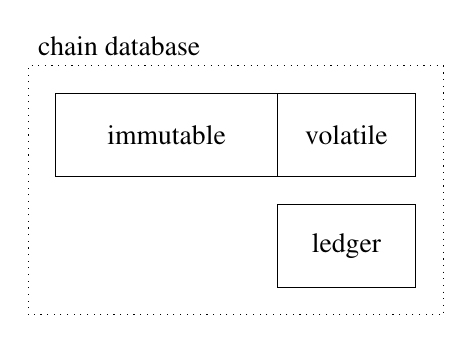
\begin{tikzpicture}
\draw [dotted]
     (-50pt, -65pt)
  -- ++(0, 90pt) node[above right] {chain database}
  -- ++(150pt, 0)
  -- ++(0, -90pt)
  -- cycle;
\node [draw, shape=rectangle, minimum width=80pt, minimum height=30pt] at (0,0)  {immutable};
\node [draw, shape=rectangle, minimum width=50pt, minimum height=30pt] at (65pt, 0)  {volatile};
\node [draw, shape=rectangle, minimum width=50pt, minimum height=30pt] at (65pt, - 40pt) {ledger};
\end{tikzpicture}

Discuss the immutable/volatile split (we reference this section for that).

\section{In memory}
\label{storage:inmemory}

TODO: After we discussed the overview, we should give an overview of everything
we store in memory in any component, so that we have a better understanding of
memory usage of the chain DB as a whole.

\subsection{Chain fragments}
\label{storage:fragments}

\subsection{Extended ledger state}
\label{storage:extledgerstate}
\label{storage:headerstate}

TODO: Is there a more natural place to talk about this? Introducing the
header state when introducing the storage layer does not feel quite right.
The storage layer might be storing the header state, but that doesn't
explain its existence.

ChainDepState, (ChainIndepState), LedgerState, ExtLedgerState

\newcommand{\timeconv}[2]{\ensuremath{\mathtt{Conv}_{#1}(#2)}}
\newcommand{\applyBlocks}[2]{\ensuremath{\mathtt{apply}_\mathit{#1}(#2)}}
\newcommand{\ledgertip}[1]{\ensuremath{\mathtt{tip}(#1)}}
\newcommand{\switch}[3]{\ensuremath{\mathtt{switch}_{(\mathit{#1},\;\mathit{#2})}(#3)}}

\chapter{Time}
\label{time}

\section{Introduction}
\label{time:introduction}

A fundamental property of the Ouroboros family of consensus protocols is that
they all divide time into discrete chunks called \emph{slots}; typically the
duration of a slot is on the order of seconds. In most Ouroboros protocols slots
are grouped into \emph{epochs}, with certain changes to the consensus chain
state happening at various points in an epoch. All nodes running the blockchain
agree on a \emph{system start time} (as a UTC time) through the chain's genesis
configuration, making the translation from a particular wallclock time to a slot
number easy: subtract the system start time from the wall clock time, and
divide by the slot length. This assumption that the mapping between wall clock
and slot or epoch numbers is always available permeated the consensus layer.
Unfortunately, it is not a valid assumption in the presence of hard forks.

It's not difficult to illustrate this with an example. Suppose we want to know
which slot time $t$ corresponds to in:
%
\begin{center}
\begin{tikzpicture}
\draw (0,0) -- (330pt, 0);
\draw [dotted] (180pt,20pt) node[above] {era transition} -- (180pt,-30pt);
\node at (273 pt,0) {$\bullet$};
\node at (273 pt,0) [above] {$t$};
% era 1
% slot length 6
% epoch size 10
% 3 epochs
\foreach \x in {0, 6, ..., 180} {
  \draw (\x pt, 0) -- +(0, -3pt);
}
\foreach \x in {0, 60, ..., 180} {
  \draw (\x pt, 0) -- +(0, -10pt);
}
% era 2
% slot length 3
% epoch size 16
% 3+ epochs
\foreach \x in {180, 183, ..., 330} {
  \draw (\x pt, 0) -- +(0, -3pt);
}
\foreach \x in {180, 228, ..., 330} {
  \draw (\x pt, 0) -- +(0, -10pt);
}
\end{tikzpicture}
\end{center}
%
We can read off from this depiction that $t$ is in epoch 1 \emph{of the second
era}, and relative slot 14 within that epoch. Since there are 16 slots to an
epoch in that era, that makes it slot $1 \times 16 + 14 = 30$ within that era.
The second era was preceded by three epochs in the first era, each of which
contained 10 slots, which means that time $t$ was slot $3 \times 10 + 30 = 60$
globally.

But now consider how this calculation changes if the era transition would have
happened one epoch later:
%
\begin{center}
\begin{tikzpicture}
\draw (0,0) -- (330pt, 0);
\draw [dotted] (240pt,20pt) node[above] {era transition} -- (240pt,-30pt);
\node at (273 pt,0) {$\bullet$};
\node at (273 pt,0) [above] {$t$};
% era 1
% slot length 6
% epoch size 10
% 4 epochs
\foreach \x in {0, 6, ..., 240} {
  \draw (\x pt, 0) -- +(0, -3pt);
}
\foreach \x in {0, 60, ..., 240} {
  \draw (\x pt, 0) -- +(0, -10pt);
}
% era 2
% slot length 3
% epoch size 16
% 1+ epochs
\foreach \x in {240, 243, ..., 330} {
  \draw (\x pt, 0) -- +(0, -3pt);
}
\foreach \x in {240, 288, ..., 330} {
  \draw (\x pt, 0) -- +(0, -10pt);
}
\node at (273 pt,0) {$\bullet$};
\node at (273 pt,0) [above] {$t$};
\end{tikzpicture}
\end{center}
%
Slot $t$ is now in epoch 0 of the second era, with relative
slot 11, making it slot $0 \times 16 + 11 = 11$ within the second era.
Since the second era got preceded by \emph{four} epochs of the first era,
that makes time $t$ global slot $4 \times 10 + 11 = 51$.

All of this would be no more than a minor complication if the exact moment of
the era transition would be statically known. This however is not the case: the
moment of the era transition is decided \emph{on the chain itself}. This leads
to the inevitable conclusion that time/slot conversions depend on the ledger
state, and may indeed be impossible: the slot at time $t$ is \emph{simply not
yet known} if the transition to era 2 has not been decided yet.

\section{Slots, blocks and stability}
\label{time:slots-vs-blocks}

In \cref{consensus:overview:k} we discussed the fundamental parameter $k$:
blocks that are more than $k$ blocks away from the tip of the chain are
considered to be immutable by the consensus layer and no longer subject to
rollback. We say that such blocks are \emph{stable}.

The ledger layer itself also depends on stability; for example, in Shelley the
stake distribution to be used for the leadership check needs to be stable before
it is adopted (this avoids malicious nodes from inspecting the leadership
schedule and then trying to cause a rollback if that leadership schedule is not
beneficial to them).

The ledger layer however does not use block numbers to determine stability, but
uses slot numbers to approximate it instead. This ultimately comes from the fact
that in Ouroboros the length of an \emph{epoch} is based on slots, not blocks,
although this is something we may wish to revisit (\cref{future:block-vs-slot}).

Depending on the particular choice of consensus algorithm, not all slots contain
blocks. For example, in Praos only a relatively small percentage of slots
contain blocks, depending on the Praos $f$ parameter (in Shelley, $f$ is set to
5\%). However,  the various Ouroboros protocols come with proofs (actually, a
probabilistic argument) providing a window of a certain number of slots that is
guaranteed to contain at least $k$ blocks; for example, for Ouroboros Classic
that window is $2k$ slots\footnote{Without much justification, we adopt this
same window for PBFT as well. It is almost certainly a gross overestimation.},
and for Ouroboros Praos that window is $3k/f$. Stability requirements in the
ledger then take the form ``at least $3k/f$ slots must have passed'' instead of
``at least $k$ blocks must have been applied''.

\section{Definitions}

\subsection{Time conversion}

As we saw in \cref{time:introduction}, we cannot do time conversions independent
of a ledger state. This motivates the following definition:

\begin{definition}[Time conversion]
Let $\timeconv{\sigma}{t}$ be the function that converts time $t$, with $t$
either specified as a wallclock time, a slot number, or an epoch number, to a
triplet
\begin{center}
(wallclock time, slot number, epoch number)
\end{center}
using ledger state $\sigma$, provided $\sigma$ contains sufficient information
to do so; $\timeconv{\sigma}{t}$ is undefined otherwise.
\end{definition}

Since all past era transitions are (obviously) known, time conversion should
always be possible for points in the past. Let $\ledgertip{\sigma}$ be the (time
of) the most recently applied block in $\sigma$. Then:

\begin{property}[Conversion for past points]
$\timeconv{\sigma}{t}$ should be defined for all $t \le \ledgertip{\sigma}$.
\end{property}

Furthermore, we assume that time conversion is monotone:

\begin{property}[Monotonicity of time conversion]
\label{time-conversion-monotone}
If $\timeconv{\sigma}{t}$ is defined, then $\timeconv{\applyBlocks{bs}{\sigma}}{t}$ must be as well and
\begin{equation*}
\timeconv{\applyBlocks{bs}{\sigma}}{t} = \timeconv{\sigma}{t}
\end{equation*}
\end{property}
%
where $\applyBlocks{bs}{\sigma}$ denotes the ledger state after applying blocks
$\mathit{bs}$.

\subsection{Forecast range}

Under certain conditions a ledger state may be usable to do time conversions
for slots ahead of the ledger state.

\begin{definition}[Forecast range]
We say that time $t > \ledgertip{\sigma}$ is within the forecast range of
$\sigma$ if \timeconv{\sigma}{t} is defined.
\end{definition}

Note that monotonicity (\cref{time-conversion-monotone}) should still
apply.

\subsection{Safe zone}

In order to be able to have a non-empty forecast range, we need to restrict
when era transitions can occur.

\begin{definition}[Safe zone]
A \emph{safe zone} is a period of time ahead of a ledger's tip in which an
era transition is guaranteed not to occur if it is not yet known.
\end{definition}

Intuitively, a non-empty safe zone means that there will be time between an
era transition being announced and it happening, no matter how the chain
is extended (no matter which blocks are applied):
%
\begin{equation}
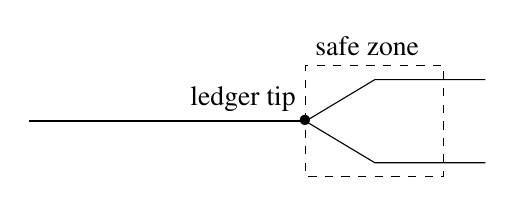
\begin{tikzpicture}[baseline=0pt]
\draw [thick] (-50pt,0) -- (50pt, 0) coordinate (tip);
\draw (tip) -- ++(25pt,  15pt) -- ++(40pt, 0pt);
\draw (tip) -- ++(25pt, -15pt) -- ++(40pt, 0pt);
\node at (tip) {$\bullet$};
\node at (tip) [above left] {ledger tip};
\draw [dashed] (tip)
            -- ++(0pt, 20pt) node[above right] {safe zone}
            -- ++(50pt, 0pt) -- ++(0pt, -40pt) -- ++(-50pt, 0pt) -- cycle;
\end{tikzpicture}
\end{equation}

\section{Ledger restrictions}
\label{time:ledgerrestrictions}

\subsection{Era transitions must be stable}

Monotonicity (\cref{time-conversion-monotone}) only talks about a chain's linear
history; since the consensus layer needs to deal with rollbacks (switching to
alternative chains) too, we will actually need a stronger property. Clearly,
time conversions cannot be invariant under switching to arbitrary chains; after
all, alternative chains might have era transitions in different places. The
consensus layer however does not \emph{support} switching to arbitrary
alternative chains; we have a maximum rollback (\cref{consensus:overview:k}),
and we never switch to a shorter chain (\cref{consensus:overview:chainsel},
\cref{never-shrink}). This means that we can model switching to an alternative
chain as $$\switch{n}{bs}{\sigma}$$ where $n \le k$ indicates how many blocks we
want to rollback, $\mathit{bs}$ is a list of new blocks we want to apply, and
$\mathtt{length} \; \mathit{bs} \ge n$.

\begin{property}[Time conversions stable under chain evolution]
\label{time-stable-under-evolution}
If \timeconv{\sigma}{t} is defined, then so is
\timeconv{\switch{n}{bs}{\sigma}}{t}
and moreover
\begin{equation*}
  \timeconv{\sigma}{t}
= \timeconv{\switch{n}{bs}{\sigma}}{t}
\end{equation*}
\end{property}

Intuitively, \cref{time-stable-under-evolution} says that we might not be able
to do time conversion for some time $t$ because it's outside our current forecast
range, but \emph{if} it is within forecast range, then we don't need to earmark
the answers we get from conversion as ``subject to rollback'': either we don't
know, or we know for sure. This requirement may not be strictly \emph{required}
for consensus to operate (\cref{future:relax-time-requirements}), but it is
a useful assumption which simplifies reasoning about time both within consensus
and within clients of the consensus layer such as the wallet.

The existence of safe zones is not sufficient to establish this stronger
property, in two ways:

\begin{itemize}
\item If we switch from a chain where an era transition is already known but
far in the future, to a chain on which the era transition happens much sooner
(or indeed, to a chain on which the era transition is not yet known), then
the forecast range will shrink and hence
\timeconv{\switch{n}{bs}{\sigma}}{t}
might not be defined, even if \timeconv{\sigma}{t} is.
\item Conversely, if we switch from a chain on which the era transition is
happening relatively soon, to a chain on which the era transition is happening
later, then the forecast range will not shrink, but the time conversions on
both chains will not agree with each other.\footnote{Going from a
chain on which the era transition is not yet known to one in which it \emph{is}
known is not problematic, due to safe zones.}
\end{itemize}

The key problem is that switching to an alternative chain can change our
information about future era transitions, and hence result in different time
conversions. We therefore insist that an era transition is not considered
``known'' until the block confirming the era transition is stable (no longer
subject to rollback). This means that the minimum distance from the announcement
of the era transition to the actual era transition must be long enough to
guarantee $k$ blocks plus the width of the safe zone:
%
\begin{equation}
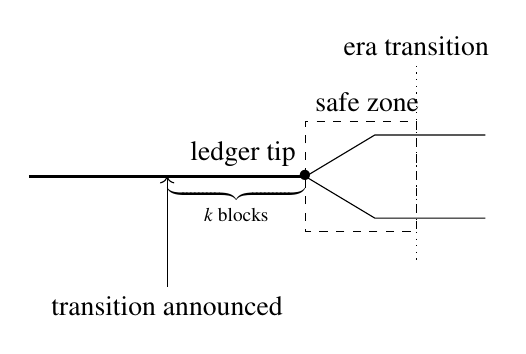
\begin{tikzpicture}[baseline=0pt]
\draw [thick] (-50pt,0) -- (50pt, 0) coordinate (tip);
\draw (tip) -- ++(25pt,  15pt) -- ++(40pt, 0pt);
\draw (tip) -- ++(25pt, -15pt) -- ++(40pt, 0pt);
\node at (tip) {$\bullet$};
\node at (tip) [above left] {ledger tip};
\draw [dashed] (tip)
            -- ++(0pt, 20pt) node[above right] {safe zone}
            -- ++(40pt, 0pt) coordinate (transition)
            -- ++(0pt, -40pt) -- ++(-40pt, 0pt) -- cycle;
\draw [dotted] (transition) ++(0pt, 20pt) node[above] {era transition}
            -- ++(0pt, -70pt);
\draw [<-] (tip) ++(-50pt, 0)
        -- +(0,-40pt) node[below] {transition announced};
% again, cheating...
\node at (25pt, -10pt) {$\underbrace{\hspace{50pt}}_\textrm{$k$ blocks}$};
\end{tikzpicture}
\end{equation}
%
How many slots are required to guarantee at least $k$ blocks is consensus
protocol specific; for example, for Praos this is typically set to $3k/f$ slots,
where $f$ is the active slot coefficient.

Many ledgers set the width of the safe zone such that it guarantees at least $k$
blocks, but \emph{in principle} there is no need for the width of the safe zone
to be related to $k$ at all, although other parts of consensus might have
requirements for the width of the safe zone; we will discuss that in the next
section (\cref{time:ledgerrestrictions:safezones}).

\subsection{Size of the safezones}
\label{time:ledgerrestrictions:safezones}

The most important example of where we might need to do time translation for
blocks ahead of the ledger's tip is forecasting the Shelley ledger view
(\cref{ledger:forecasting}). The Shelley ledger view contains an abstraction
called \lstinline!EpochInfo! allowing the ledger to do time conversions, for
example to decide when rewards should be allocated.

As discussed in \cref{forecast:ledgerview}, it is important that the forecast
range of the ledger to allow us to validate at least $k + 1$ blocks after the
ledger tip; consequently, the safe zone of the ledger must be wide enough to
guarantee that it can span $k + 1$ blocks. This combination of the requirements
of the ledger with the header/body split
(\cref{nonfunctional:network:headerbody}) means that in practice the width of
the safe zone should be at least equal to the forecast range of the ledger, and
hence defined in terms of $k$ after all.

\subsection{Stability should not be approximated}

We discussed in \cref{time:slots-vs-blocks} that the ledger uses uses slot
numbers to approximate stability. Such an approximation would violate
\cref{time-stable-under-evolution}, however. Although we never switch to a
shorter chain in terms of blocks, it is certainly possible that we might switch
to a chain with a smaller \emph{slot} number at its tip: this would happen
whenever we switch to a longer but denser chain. If stability would be based on
slot numbers, this might mean that we could go from a situation in which the era
transition is considered known (and hence the forecast extends into the next
era) to a situation in which the era transition is not yet considered known (and
hence the forecast range only includes the safe zone in the current era).

Admittedly such a reduction of the forecast range would be temporary, and once
the era transition is considered known again, it will be in the same location;
after all, the block that confirmed the era transition \emph{is} stable. This
means that any previously executed time conversions would remain to be valid;
however, the fact that the forecast range shrinks might lead to unexpected
surprises. The consensus layer therefore does not use the ledger's layer
notion of stability, but instead maintains additional state so that it can use
\emph{block} numbers rather than slot numbers to determine stability and be
able to determine stability precisely rather than approximate it.

\section{Properties}

\subsection{Forecast ranges arising from safe zones}

Slot length and epoch size can only change at era transitions. This means that
if the transition to the next era is not yet known, any time $t$ within the
era's safe zone is guaranteed to be within the era's forecast range. If the
transition to the next era \emph{is} known, the safe zone of the current era is
not relevant, but the safe zone of the next era is:
%
\begin{equation}
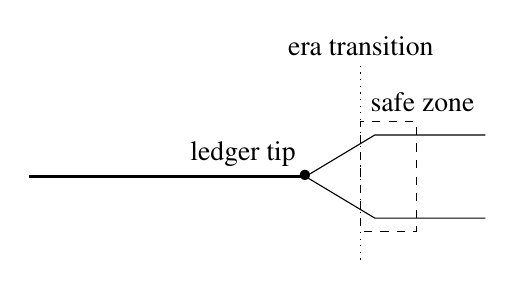
\begin{tikzpicture}[baseline=0pt]
\draw [thick] (-50pt,0) -- (50pt, 0) coordinate (tip);
\draw (tip) -- ++(25pt,  15pt) -- ++(40pt, 0pt);
\draw (tip) -- ++(25pt, -15pt) -- ++(40pt, 0pt);
\node at (tip) {$\bullet$};
\node at (tip) [above left] {ledger tip};
\draw [dashed] (tip) ++(20pt, 0pt) coordinate (transition)
            -- ++(0pt, 20pt) node[above right] {safe zone}
            -- ++(20pt, 0pt) -- ++(0pt, -40pt) -- ++(-20pt, 0pt) -- cycle;
\draw [dotted] (transition) ++(0pt, 40pt) node[above] {era transition}
            -- ++(0pt, -70pt);
\end{tikzpicture}
\end{equation}
%
The safe zone of the next era might be smaller or larger than (or indeed of
equal size as) the safe zone of the previous era; in this example it happens to
be smaller.

\Cref{hfc:era-transition-becoming-known} shows how the forecast range changes as
the next era transition becomes known; as shown, the next era starts at the
earliest possible moment (right after the safe zone); in general it could start
later than that, but of course not earlier (that would violate the definition of
the safe zone).

\begin{figure}

\begin{equation}
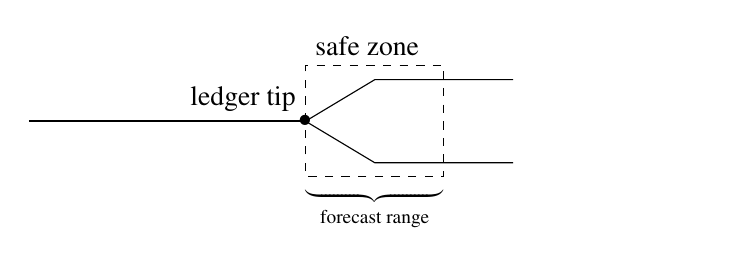
\begin{tikzpicture}[baseline=0pt]
\path (0,0) -- ++(200pt, 0pt); % adjust bounding box
\draw [thick] (-50pt,0) -- (50pt, 0) coordinate (tip);
\draw (tip) -- ++(25pt,  15pt) -- ++(50pt, 0pt);
\draw (tip) -- ++(25pt, -15pt) -- ++(50pt, 0pt);
\node at (tip) {$\bullet$};
\node at (tip) [above left] {ledger tip};
\draw [dashed] (tip)
            -- ++(0pt, 20pt) node[above right] {safe zone}
            -- ++(50pt, 0pt)
            -- ++(0pt, -40pt)
            -- ++(-50pt, 0pt) coordinate[pos=0.5] (safezone)
            -- cycle;
\node at (safezone) [below] {$\underbrace{\hspace{50pt}}_\textrm{forecast range}$};
\end{tikzpicture}
\end{equation}

\begin{equation}
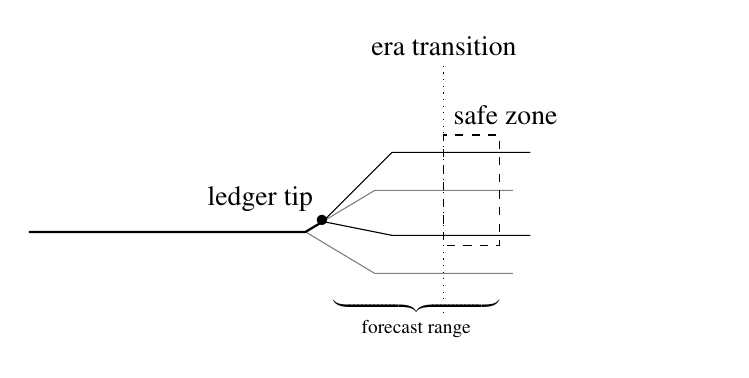
\begin{tikzpicture}[baseline=0pt]
\path (0,0) -- ++(200pt, 0pt); % adjust bounding box
\draw [gray] (-50pt,0) -- (50pt, 0) coordinate (oldtip);
\draw [gray, name path=chaintop] (oldtip) -- ++(25pt, 15pt) coordinate[pos=0.25] (tip) -- ++(50pt, 0pt);
\draw [gray] (oldtip) -- ++(25pt, -15pt) -- ++(50pt, 0pt);
\draw [thick] (-50pt,0) -- (50pt, 0) -- (tip);
\node at (tip) {$\bullet$};
\node at (tip) [above left] {ledger tip};
\draw (tip) -- ++(25pt, 25pt) -- +(50pt, 0pt);
\draw (tip) -- ++(25pt, -5pt) -- +(50pt, 0pt);
\draw [dotted, name path=transition]
        (oldtip) ++(50pt, 60pt) node[above] {era transition}
              -- ++(0pt, -90pt);
\path [name intersections={of=transition and chaintop}]
        (intersection-1) coordinate (safezone);
\draw [dashed] (safezone)
            -- ++(0pt, 20pt) node[above right] {safe zone}
            -- ++(20pt, 0pt)
            -- ++(0pt, -40pt)
            -- ++(-20pt, 0pt) coordinate[pos=0.5] (safezone)
            -- cycle;

% cheat: we should compute this of course :)
\node at (90pt,-20pt) [below] {$\underbrace{\hspace{60pt}}_\textrm{forecast range}$};
\end{tikzpicture}
\label{forecast-range-known-era-transition}
\end{equation}
\caption{\label{hfc:era-transition-becoming-known}Era transition becoming known}
\end{figure}

\subsection{Cross-fork conversions}
\label{time:cross-fork}

\begin{lemma}[Cross fork conversions]
Suppose we have the ledger state at some point $P$, and want to do time
conversions for time $t$ of a point $Q$ on a different fork of the chain:

\begin{center}
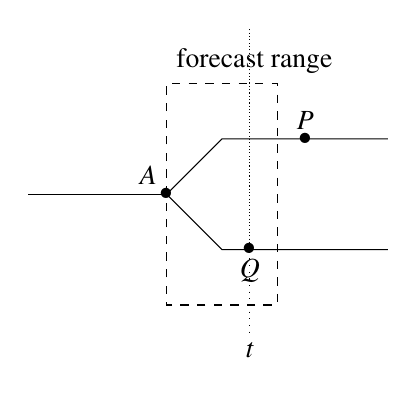
\begin{tikzpicture}
\draw (0,0) -- (50pt, 0) coordinate (A);
\draw (A) -- ++(20pt, 20pt)
          -- ++(30pt, 0) coordinate(P)
          -- ++(30pt, 0);
\draw (A) -- ++(20pt, -20pt)
          -- ++(10pt, 0) coordinate(Q1)
          -- ++(40pt, 0) coordinate(Q2)
          -- ++(10pt, 0);
\node at (A) {$\bullet$};
\node at (A) [above left] {$A$};
\node at (P) {$\bullet$};
\node at (P) [above] {$P$};
\node at (Q1) {$\bullet$};
\node at (Q1) [below] {$Q$};
\draw [dashed] (A) -- ++(0, 40pt) node[above right] {forecast range}
                   -- ++(40pt, 0)
                   -- ++(0, -80pt)
                   -- ++(-40pt, 0)
                   -- cycle;
\draw [dotted] (Q1) -- +(0, 80pt) -- +(0, -30pt) node[below] {$t$};
\end{tikzpicture}
\end{center}

Provided that $Q$ is within the forecast range of the common ancestor $A$
of $P$ and $Q$, the ledger state at $P$ can be used to do time conversions
for point $t$.
\end{lemma}

\begin{proof}
Since $t$ is within the forecast range at $A$, by definition $\timeconv{A}{t}$
is defined. By monotonicity (\cref{time-conversion-monotone}) we must have
\begin{align*}
\timeconv{A}{t} & = \timeconv{P}{t} \\
\timeconv{A}{t} & = \timeconv{Q}{t}
\end{align*}
It follows that $\timeconv{P}{t} = \timeconv{Q}{t}$.
\end{proof}

\section{Avoiding time}
\label{hfc:avoiding-time}

Time is complicated, and time conversions were pervasive throughout the
consensus layer. Despite the exposition above and the increased understanding,
we nonetheless have attempted to limit the use of time as much as possible,
in an attempt to simplify reasoning whenever possible. The use of
time within the core consensus layer is now very limited indeed:

\begin{enumerate}
\item When we check if we are a slot leader and need to produce a block, we
need to know the current time as a slot number (\todo{TODO.}We should discuss
this somewhere. The chapter on the consensus protocol discusses the protocol
side of things, but not the actual ``fork block production'' logic.)
\item When we add new blocks to the chain DB, we need to check if their slot
number is ahead of the wallclock (\cref{chainsel:infuture}).
\item Specific consensus protocols may need to do time conversions; for example,
Praos needs to know when various points in an epoch have been reached in order
to update nonces, switch stake distribution, etc.
\end{enumerate}

None of these use cases require either forecasting or cross-chain conversions.
The most important example of where forecasting is required is in projecting
the ledger view, as discussed in \cref{time:ledgerrestrictions:safezones}.
Cross-fork conversions (\cref{time:cross-fork}) may arise for example when the consensus layer makes time conversions available to tooling such as the wallet,
which may use it for example to show the wallclock of slots of blocks that may
not necessarily live on the current chain.

Keeping track of era transitions, and providing time conversions that take
them into account, is the responsibility of the hard fork combinator and
we will discuss it in more detail in \cref{hfc:time}.

In the remainder of this section we will discuss some simplifications
that reduced the reliance on time within the consensus layer.

\subsection{``Header in future'' check}
\label{time:header-infuture-check}

Recall from \cref{nonfunctional:network:headerbody} that block downloading
proceeds in two steps: first, the chain sync client downloads the block header
and validates it; if it finds that the header is valid, the block download logic
may decide to also download the block body, depending on chain selection
(\cref{consensus:overview:chainsel,consensus:class:chainsel}).

Suppose the node's own ledger state is at point $P$, and the incoming header is
at point $Q$. In order to validate the header, we need a ledger \emph{view} at
point $Q$ without having the ledger \emph{state} at point $Q$; this means that
point $Q$ must be within the ledger's forecast range at the common ancestor $A$
of $P$ and $Q$ (\cref{,ledger:forecasting}):

\begin{center}
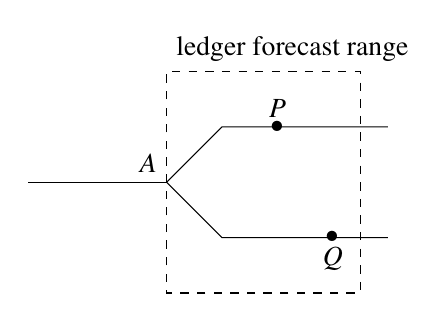
\begin{tikzpicture}
\draw (0, 0) -- (50pt, 0) coordinate (A);
\draw (A) -- ++(20pt,  20pt) -- ++(20pt, 0) coordinate (P) -- ++(40pt, 0);
\draw (A) -- ++(20pt, -20pt) -- ++(40pt, 0) coordinate (Q) -- ++(20pt, 0);
\node at (P) {$\bullet$};
\node at (Q) {$\bullet$};
\node at (A) [above left] {$A$};
\node at (P) [above] {$P$};
\node at (Q) [below] {$Q$};
\draw [dashed] (A) -- ++(0, 40pt) node[above right] {ledger forecast range}
                   -- ++(70pt, 0)
                   -- ++(0, -80pt)
                   -- ++(-70pt, 0)
                   -- cycle;
\end{tikzpicture}
\end{center}

As we have seen in \cref{time:cross-fork}, if $Q$ is within the \emph{time}
forecast range at $A$---put another way, if the time forecast range is at least
as wide as the ledger forecast range---then we also can use the ledger state at
$P$ to do time conversions at point $Q$. Moreover, as we saw in
\cref{time:ledgerrestrictions:safezones}, for many ledgers that inclusion
\emph{must} hold. If we make this a requirement for \emph{all} ledgers, in
principle the chain sync client could do a header-in-future check.

For simplicity, however, we nonetheless omit the check. As we will see in the
next section, the chain database must repeat this check \emph{anyway}, and so
doing it ahead of time in the chain sync client does not help very much;
skipping it avoids one more use of time within the consensus layer. Indeed, a
case could be made that we could skip header validation altogether, which would
alleviate the need for forecasting \emph{at all}; we will come back to this in
\cref{future:eliminating-forecasting}.

\subsection{Ahead-of-time ``block in future'' check}
\label{time:block-infuture-check}

In the original design of the chain database, when a new block was added we
first checked if the block's slot number was ahead of the wallclock, before
considering it for chain selection. If it was ahead of the wallclock by a small
amount (within the permissible clock skew), we then scheduled an action to
reconsider the block when its slot arrived.

In order to compare the block's slot number to the wallclock, we can either
convert the block's slot to a wallclock time, or convert the current wallclock
time to a slot number. Both are problematic: the only ledger state we have
available is our own current ledger state, which may not be usable to translate
the current wallclock time to a slot number, and since we don't know anything
about the provenance of the block (where the block came from), that ledger state
may also not be usable to translate the block's slot number to a wallclock time.
We now circumvent this problem by delaying the in-future check until we have
validated the block,\footnote{One might worry about vulnerability to a DoS
attack, but the scope for an adversary to flood us with blocks from the future
is limited, for two reasons. First, we still \emph{validate} all headers, and
the forecast range will determine quite how far we can look ahead. Second, the
moment that the adversary feeds us with enough blocks from the future that their
chain becomes longer than our own, we will download the corresponding
blocks, find that they are from the future, mark them as invalid (provided it
exceeds clock skew) and disconnect from the peer which we now consider to be
potentially adversarial.} and so can use the block's \emph{own} ledger state to
do the time conversion (\cref{chainsel:infuture}).

We saw in the previous section that the chain sync client \emph{could} do the
in-future check on headers, but the chain sync client is not the only way that
blocks can be added to the chain database, so simply skipping the check in the
chain database altogether, stipulating as a \emph{precondition} that the block
is not ahead of the wallclock, is not a good idea. Nonetheless it is worth
considering if we could use a weaker precondition, merely requiring that the
node's current ledger tip must be usable for time conversions for the slot
number of the new block. Specifically, can we guarantee that we can satisfy this
precondition in the chain sync client, if we do the in-future check on headers
after all?

It turns out that in general we cannot, not even in relatively common cases.
Consider again the diagram from \cref{time:header-infuture-check}, but
specialised to the typical case that the upstream node is on the same chain as
we are, but a bit ahead of us:

\begin{center}
\begin{tikzpicture}
\path (0,0) -- ++(200pt, 0pt); % adjust bounding box
\draw (0, 0) -- (50pt, 0) coordinate (A) coordinate (P);
\draw (A) -- ++(20pt, 0pt) -- ++(20pt, 0) -- ++(40pt, 0);
\draw (A) -- ++(20pt, 0pt) -- ++(40pt, 0) coordinate (Q) -- ++(20pt, 0);
\node at (P) {$\bullet$};
\node at (Q) {$\bullet$};
\node at (A) [above left] {$A$};
\node at (A) {$\bullet$};
\node at (P) [below left] {$P$};
\node at (Q) [below] {$Q$};
\draw [dashed] (A) -- ++(0, 20pt) node[above right] {forecast range}
                   -- ++(70pt, 0)
                   -- ++(0, -40pt)
                   -- ++(-70pt, 0)
                   -- cycle;
\end{tikzpicture}
\end{center}

Since $P$ and $Q$ are on the same chain,  point $P$ is necessarily also the
``intersection'' point, and the distance between $P$ and $Q$ can only arise from
the block download logic lagging behind the chain sync client.
Now consider what happens when the node switches to an alternative fork:

\begin{center}
\begin{tikzpicture}
\path (0,0) -- ++(200pt, 0pt); % adjust bounding box
\draw (0, 0) -- (30pt, 0) coordinate (A);
\draw (A) -- ++(20pt,  20pt) -- ++(20pt, 0) coordinate (P) -- ++(60pt, 0);
\draw (A) -- ++(20pt, -20pt) -- ++(60pt, 0) coordinate (Q) -- ++(20pt, 0);
\node at (P) {$\bullet$};
\node at (Q) {$\bullet$};
\node at (A) [above left] {$A$};
\node at (P) [above] {$P$};
\node at (Q) [below] {$Q$};
\draw [dashed] (A) -- ++(0, 40pt) node[above right] {forecast range}
                   -- ++(70pt, 0)
                   -- ++(0, -80pt)
                   -- ++(-70pt, 0)
                   -- cycle;
\end{tikzpicture}
\end{center}

Note what happens: since the node is switching to another fork, it must rollback
some blocks and then roll forward; consequently, the intersection point $A$
moves back, and $P$ moves forward (albeit on a different chain). $Q$ stays the
same, \emph{but might have fallen out of the forecast range at $A$}.

This means that even if the chain sync client was able to verify that a header
(at point $Q$) was not ahead of the wallclock, if the node switches to a
different fork before the block download logic has downloaded the corresponding
block, when it presents that downloaded block to the chain database, the block
might no longer be within the forecast range of the node's current ledger and
the chain database will not be able to verify (ahead of time) whether or not the
block is ahead of the wallclock. What's worse, unlike the chain sync client, the
chain database has no access to the intersection point $A$; it all it has is the
ledger's current tip at  point $P$ and the new block at point $Q$. It therefore
has no reliable way of even determining \emph{if} it can do time conversions for
the new block.

\subsection{``Immutable tip in future'' check}
\label{time:imm-tip-in-future}

The chain database never adopts blocks from the future
(\cref{chainsel:infuture}). Nevertheless, it is possible that if the user sets
their computer system clock back by (the equivalent of) more than $k$ blocks,
the immutable database (\cref{storage:components}) might contain blocks
whose slot numbers are ahead of the wall clock. We cannot verify this during a
regular integrity check of the immutable database because, as we have seen in
this chapter, we would need a ledger state to do so, which we are not
constructing during that integrity check. For now, we simply omit this check
altogether, declaring it to be the user's responsibility instead to do a
fresh install if they do reset their clock by this much.

However, in principle this check is not difficult: we initialise the immutable
DB \emph{without} doing the check, then initialise the ledger DB, passing it the
immutable DB (which it needs to replay the most recent blocks, see
\cref{ledgerdb}), and then ask the ledger DB for the ledger state
corresponding to the tip of the immutable database. That ledger state will then
allow us to do time conversions for any of the blocks in the immutable DB,
trimming any blocks that are ahead of the wallclock.

\subsection{Scheduling actions for slot changes}
\label{time:scheduling-actions}

The consensus layer provides an abstraction called \lstinline!BlockchainTime!
that provides access to the current slot number. It also offers an interface for
scheduling actions to be run on every slot change. However, if the node is still
syncing with the chain, and does not have a recent ledger state available, the
current slot number, and indeed the current slot length, are simply unknown:
when the node uses its current ledger state to  try and convert the current
wallclock to a slot number, it will discover that  the current wallclock is
outside the ledger's forecast range. In this case the blockchain time will
report the current slot number as unavailable, and any scheduled actions will
not be run.

We therefore limit the use of this scheduler to a single application only:
it is used to trigger the leadership check (and corresponding block
production, if we find we are a leader). This means that the leadership
check will not be run if we are still syncing with the chain and have no
recent ledger state available, but that is correct: producing blocks based on
ancient ledger states is anyway not useful.

\subsection{Switching on ``deadline mode'' in the network layer}

Under normal circumstances, the priority of the network layer is to reduce
\emph{latency}: when a block is produced, it must be distributed across the
network as soon as possible, so that the next slot leader can construct the
\emph{next} block as this block's successor; if the block arrives too late,
the next slot leader will construct their block as the successor of the previous
block instead, and the chain temporarily forks.

When we are far behind, however, the priority is not to reduce latency, but
rather to improve \emph{throughput}: we want to catch up as quickly as we can
with the chain, and aren't producing blocks anyway
(\cref{time:scheduling-actions}).

In order to switch between these two modes we want to know if we are near the
tip of the ledger---but how can we tell? If we know the current slot number
(the slot number corresponding to the current wall clock), we can compare
that current slot number to the slot number at the tip of the ledger. But,
as we mentioned before, if we are far behind, the current slot number is
simply unknown. Fortunately, we can use this to our advantage: if the
slot number is unknown, we \emph{must} be far behind, and hence we can use
the decision, turning on deadline mode only if the slot number is known
\emph{and} within a certain distance from the ledger tip.

\chapter{Miscellaneous}

TODO\todo{TODO}: This is a mess at the moment.

\section{On abstraction}

ledger integration: as things were changing a lot, it made sense for consensus to define the ledger API internally and have the integration be done consensus side. but as things are stabilising, it might make more sense for that abstraction to live externally, so that you can literally plug in Shelley into consensus and we don't have to do anything

\section{On-disk ledger state}

\duncan

Sketch out what we think it could look like
Consequences for the design

\section{Transaction TTL}
\label{future:ttl}

Describe that the mempool could have explicit support for TTL, but that right now we don't (and why this is OK: the ledger anyway checks tx TTL). We should discuss why this is not an attack vector (transactions will either be included in the blockchain or else will be chucked out because some of their inputs will have been used).

\section{Block based versus slot based}
\label{future:block-vs-slot}

\section{Eliminating safe zones}
\label{future:eliminating-safezones}

Are they really needed? Consensus doesn't really look ahead anymore?
(Headers are not checked for time; leadership is ticking, not forecasting).
Does the wallet really need it? What about the ledger?

Other thought: what if we split slots into "microslots", 20 microslots to a
slot. Now the slot/time mapping is \emph{always} known, and for Shelley etc
we don't actually need to know the global microslot, all we care about is
the microslot within a slot (and hence is independent of when Shelley starts).
This would make time conversion no longer state dependent.

\section{Eliminating forecasting}
\label{future:eliminating-forecasting}

This is a stronger version of \cref{future:eliminating-safezones}, where
we eliminate \emph{all} forecasting. Specifically, this means that we don't
do header validation anymore, relying on the chain DB to do block validation.
This would be an important simplification of the consensus layer, but we'd
need to analyse what the ``benefit'' of this simplification is for an
attacker. Personally, I think it'll be okay.

The most important analysis we need to do here is how this affects the memory
usage of the chain sync client. Note that we already skip the ahead-of-time
check, which we don't do until we have the full block and validate it. We
should discuss that somewhere as well.

\section{Open kinds}
\label{future:openkinds}

Avoid type errors such as trying to apply a ledger to a block instead of an era
(or an era instead of crypto, or..).

\section{Relax requirements on time conversions}
\label{future:relax-time-requirements}

Perhaps it would be okay if time conversions we strictly relative to a ledger
state, rather than ``absolute'' (\cref{time:ledgerrestrictions}).

\section{Configuration}

What a mess.

\section{Specialised chain selection data structure}

In \cref{chainsel:spec} we describe how chain selection is implemented. However,
in an ideal world this would mean we have some kind of specialised data
structure supporting

\begin{itemize}
\item Efficient insertion of new blocks
\item Efficient computation of the best chain
\end{itemize}

It's however not at all clear what such a data structure would look like if we
don't want to hard-code the specific chain selection rule.

\section{Dealing with clock changes}
\label{future:clockchanges}

When the user changes their system clock, blocks that we previously adopted
into our current chain might now be ahead of the system clock (\cref{chainsel:infuture}) and should not
be part of the chain anymore, and vice versa.

When the system clock of a node is moved \emph{forward}, we should run chain
selection again because some blocks that we stored because they were in the
future may now become valid. Since this could be any number of blocks, on any
fork, probably easiest to just do a full chain selection cycle (starting from
the tip of the immutable database).

When the clock is moved \emph{backwards}, we may have accepted blocks that we
should not have. Put another way, an attacker might have taken advantage of the
fact that the clock was wrong to get the node to accept blocks in the future. In
this case we therefore really should rollback--- but this is a weird kind of
rollback, one that might result in a strictly smaller current chain. We can only
do this by re-initialising the chain DB from scratch (the ledger DB does not
support such rollback directly). Worse still, we have have decided that some
blocks were immutable which really weren't.

Unlike the data corruption case, here we should really endeavour to get to a
state in which it was as if the clock was never ``wrong'' in the first place;
this may mean we might have to move some blocks back from the immutable DB to
the volatile DB, depending on exactly how far the clock was moved back and how
big the overlap between the immutable DB and volatile DB is.

It is therefore good to keep in mind that the overlap between the immutable DB
and volatile DB does make it a bit easier to deal with relatively small clock
changes; it may be worth ensuring that, say, the overlap is at least a few days
so that we can deal with people turning back their clock a day or two without
having to truncate the immutable database. Indeed, in a first implementation,
this may be the \emph{only} thing we support, though we will eventually have to
lift that restriction.

Right now, we do nothing special when the clock moves forward (we will discover
discover the now valid blocks on the next call to \lstinline!addBlock!
(\cref{chainsel:addblock}). When the clock is reset \emph{backwards}, the node
will currently (intentionally) crash, we make no attempt to try and reset
the state (the current slot number moving backwards might cause difficulties
in many places). Unfortunately, if the clock is moved so far back that blocks
in the \emph{immutable database} are now considered to be ahead of the wall
clock, we will not currently detect this (\cref{time:imm-tip-in-future}).


\part{Testing}

\chapter{Reaching consensus}
\label{testing:consensus}

\section{Dire-but-not-to-dire}
\label{testing:dire}

We should mention the PBFT threshold here \cref{bft-paper}.

\chapter{The storage layer}
\label{testing:storage}


\part{Future Work}

\newcommand{\RequiredPeers}{\ensuremath{N_\mathit{rs}}}

\chapter{Ouroboros Genesis}
\label{genesis}

\section{Introduction}

\subsection{Background: understanding the Longest Chain rule}
\label{genesis:background:longest-chain}

Recall the Praos chain selection rule:

\begin{definition}[Longest Chain Rule]
\label{longest-chain-rule}
A candidate chain is preferred over our current chain if
%
\begin{enumerate}
\item it is longer than our chain, and
\item the intersection point is no more than $k$ blocks away from our tip.
\end{enumerate}
\end{definition}

The purpose of chain selection is to resolve temporary forks that arise from the
normal operation of the protocol (such as when there are multiple leaders in a
single slot), and---importantly---to distinguish honest chains from chains
forged by malicious nodes. It is not a priori clear why choosing longer chains
over shorter chains would help distinguish malicious chains from honest chains:
why would an honest chain be longer?

Recall that the leadership schedule is based on stake: a node's probability of
being elected a leader in a given slot is proportional to their stake. By
assumption, the malicious nodes in the system together have less stake than the
honest nodes; security of the system as a whole critically depends on the
presence of this honest majority. This means that when a malicious node extends
the chain they can only produce a chain with relatively few filled slots: the
honest chain will be \emph{denser}. At least, this will be true near the
intersection point: as we get further away from that intersection point, the
malicious node can attempt to influence the leadership schedule for future slots
to their advantage.

The Praos security analysis \cite{cryptoeprint:2017:573} tells us that provided
all (honest) nodes are online all the time, they will all share the same chain,
except for blocks near the tips of those chains. Moreover, blocks with a slot
number ahead of the wall clock are considered invalid. This means that the only
way\footnote{The chain sync client does actually allow for some clock skew.
Headers that exceed the clock skew are however not included in chain selection.}
for one chain to be longer than another is by having more filled slots between
the tip of the shared prefix and ``now'': in other words, they must be
\emph{denser}.\footnote{A slightly subtle point arises from era transitions on
the chain that may change parameters such as the active slot coefficient,
allowing for denser chains after the transition. Although an adversary can
introduce such a transition on their own fork, such a transition would not take
effect until one stability window later, and so this won't affect the density
near the intersection point. Era transitions that are agreed on on the main
chain  benefit the honest parties and the adversary equally.}
%
\begin{center}
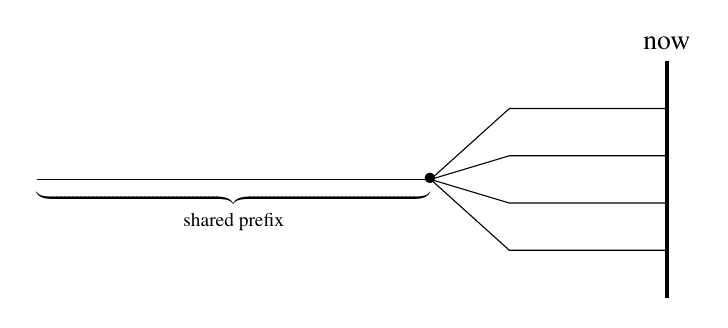
\begin{tikzpicture}
\draw (0,0) -- (5,0) coordinate(branch) node{$\bullet$} node[pos=0.5,below]{$\underbrace{\hspace{5cm}}_\text{shared prefix}$};
\draw (branch) -- ++(1,  0.9) -- ++(2,0);
\draw (branch) -- ++(1,  0.3) -- ++(2,0);
\draw (branch) -- ++(1, -0.3) -- ++(2,0);
\draw (branch) -- ++(1, -0.9) -- ++(2,0);
\draw [ultra thick] (8,-1.5) -- (8,1.5) node[above]{now};
\end{tikzpicture}
\end{center}
%
This motivates the first part of the Longest Chain rule: chain length is a
useful proxy for chain density, which in turn reflects honesty. The second part
of the rule---the intersection point is no more than $k$ blocks away from our
tip---is important because we can only meaningfully compare density \emph{near
  the intersection point}. As we get further away from the intersection point,
an adversary can start to influence the leadership schedule. This means that if
the adversary's chain forks off from the honest chain far back enough, they can
construct a chain that is longer than the honest chain. The Longest Chain rule
therefore restricts rollback, so that we will simply not even consider chains
that fork off that far back. We can still resolve minor forks that happen in the
honest chain during the normal operation of the protocol, because---so the
analysis guarantees---those will not be deeper than $k$ blocks.

\subsection{Nodes joining late}
\label{genesis:background:joining-late}

When new nodes join the network (or rejoin after having been offline for a
while), they don't have the advantage of having been online since the start of
the system, and have no sufficiently long prefix of the honest chain available.
As we saw at the end of \cref{genesis:background:longest-chain}, simply looking
at chain length is insufficient to distinguish the honest chain from malicious
chains: given enough time, an adversary can produce a chain that is longer than
the honest chain:
%
\begin{center}
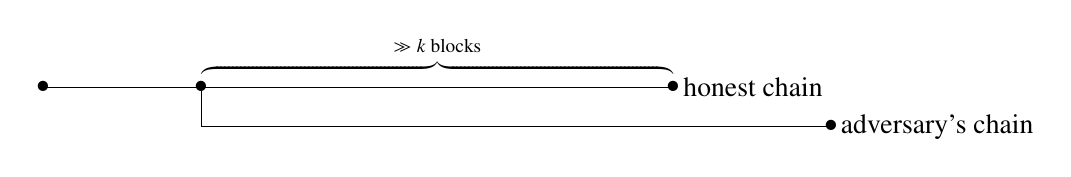
\begin{tikzpicture}[yscale=0.5]
\draw (-2,0) node{$\bullet$} -- (0,0);
\draw (0,0) node{$\bullet$} -- (6,0) node{$\bullet$} node[right] {honest chain};
\draw (0,0) -- (0,-1) -- (8,-1) node{$\bullet$} node[right]{adversary's chain};
\path (0,0) -- (6,0) node[pos=0.5, above]{$\overbrace{\hspace{6cm}}^{\text{$\gg k$ blocks}}$};
\end{tikzpicture}
\end{center}
%
When a node's current chain is somewhere along that common prefix and uses the
longest chain rule, they will choose the adversary's chain rather than the
honest chain. Moreover, they will now be unable to switch to the honest chain,
because the intersection point with that chain is more than $k$ blocks ago. If a
node would get a ``leg up'' in the form of a reliable message telling which
chain to adopt when joining the network (such a message is known as a
``checkpoint'' in the consensus literature), the Praos rule from that point
forward would prevent them from (permanently) adopting the wrong chain, but
Praos cannot be used to help nodes ``bootstrap'' when they are behind.

So far we have just been discussing Praos as it is described in theory. The
situation in practice is worse. In the abstract models of the consensus
algorithm, it is assumed entire chains are being broadcast and validated. In
reality, chains are downloaded and validated one block at a time.
We therefore don't see a candidate chain's \emph{true} length; instead, the
length of a candidate we see depends on how much of that candidate's chain we
have downloaded\footnote{Even if nodes did report their ``true length'' we would
have no way of verifying this information until we have seen the entire chain,
so we can make no use of this information for the purpose of chain selection.}.
Defining chain selection in terms of chain length, where our \emph{perceived}
chain length depends on what we decide to download, is obviously rather
circular. In terms of the above discussion, it means that the adversary's chain
doesn't even need to be longer than the honest chain:
%
\begin{center}
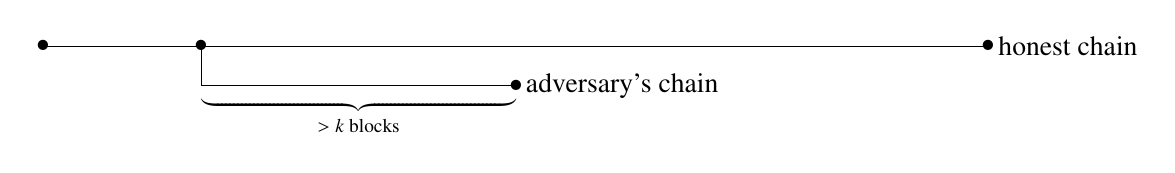
\begin{tikzpicture}[yscale=0.5]
\draw (-2,0) node{$\bullet$} -- (0,0);
\draw (0,0) node{$\bullet$} -- (10,0) node{$\bullet$} node[right] {honest chain};
\draw
   (0,0)
  -- (0,-1)
  -- (4,-1)
    node{$\bullet$}
    node[right]{adversary's chain}
    node[pos=0.5, below]{$\underbrace{\hspace{4cm}}_{\text{$> k$ blocks}}$};
\end{tikzpicture}
\end{center}
%
If the adversary's chain contains more than $k$ blocks after the intersection
point, and we \emph{happen} to download that chain first, we would adopt it and
subsequently be unable to switch to the honest chain; after all, that would
involve a rollback of more than $k$ blocks, which the Praos rule forbids.

\subsection{The Density rule}
\label{genesis:background:density-rule}

It is therefore clear that we need a different chain selection rule so that
nodes can (re)join, and the Ouroboros Genesis paper \cite{cryptoeprint:2018:378}
proposes one, shown in \cref{genesis:maxvalid-bg}. In this chapter we will work
with a slightly simplified (though equivalent) form of this rule, which we will
term the Density Rule:
%
\begin{definition}[Density Rule]
A candidate chain is preferred over our current chain if it is denser
(contains more blocks) in a window of $s$ slots anchored at the intersection
between the two chains.
\end{definition}
%
(We will briefly discuss the differences between the rule in the paper and this
one in \cref{genesis:original}.) Technically speaking, $s$ is a
parameter of the rule, but the following default is a suitable choice both from
a chain security perspective and from an implementation perspective:\footnote{If
we change the epoch size, this value might have to be reconsidered, along with
the ledger's stability window.}

\begin{definition}[Genesis window size]
The genesis window size $s$ will be set to $s = 3k/f$.
\end{definition}

Unlike the Longest Chain rule, the Density rule does not impose a maximum
rollback. It does not need to, as it always considers density \emph{at the
intersection point}. This means that in a situation such as
%
\begin{center}
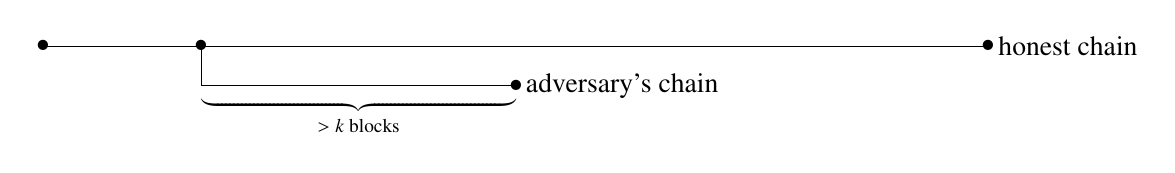
\begin{tikzpicture}[yscale=0.5]
\draw (-2,0) node{$\bullet$} -- (0,0);
\draw (0,0) node{$\bullet$} -- (10,0) node{$\bullet$} node[right] {honest chain};
\draw
     (0,0)
  -- (0,-1)
  -- (4,-1)
    node{$\bullet$} node[right]{adversary's chain}
    node[pos=0.5, below]{$\underbrace{\hspace{4cm}}_{\text{$> k$ blocks}}$};
\end{tikzpicture}
\end{center}
%
if we happen to see and adopt the adversary's chain first, we can still adopt
the honest chain (which will be denser at the intersection point, because of the
honest majority).This would however involve a rollback of more than $k$ blocks;
we will discuss how we can avoid such long rollbacks in
\cref{genesis:avoiding-long-rollbacks}.

\section{Properties of the Density rule}

In this section we will study the Density rule and prove some of its
properties. The improved understanding of the rule will be beneficial in the
remainder of this chapter.

\subsection{Equivalence to the Longest Chain rule}

For nodes that are up to date, the Density rule rule does not change how chain
selection works.

\begin{lemma}
\label{lemma:tip-density-is-chain-length}
When comparing two chains with an intersection that is at most $s$ slots away
from the two tips, the Density rule just prefers the longer chain.
\end{lemma}

\begin{proof}
The two chains share a common prefix, and differ only in the blocks
within the last $s$ slots:
%
\begin{center}
\begin{tikzpicture}[yscale=0.5]
\draw (0,0) -- (6,0) coordinate (I);
\draw (I) -- ++(1,1) -- ++(1.5,0);
\draw (I) -- ++(1,-1) -- ++ (2,0);
\draw [dashed]
    (I)
  -- ++(0, 1.5)
  -- ++(4, 0) node[pos=0.5,above]{$s$ slots}
  -- ++(0, -3)
  -- ++(-4, 0)
  -- cycle;
\end{tikzpicture}
\end{center}
%
Since the chain length in this case is simply the length of the length of the
common prefix plus the number of blocks in the window (i.e., their density),
the longer chain will also be denser in the window.

Just to be very explicit, \cref{lemma:tip-density-is-chain-length} does
\emph{not} hold when the intersection is more than $s$ slots away:
%
\begin{center}
\begin{tikzpicture}[yscale=0.5]
\draw (0,0) -- (3,0) coordinate (I);
\draw (I) -- ++(1,1) -- ++(5.5,0);
\draw (I) -- ++(1,-1) -- ++ (6,0);
\draw [dashed]
    (I)
  -- ++(0, 1.5)
  -- ++(4, 0) node[pos=0.5,above]{$s$ slots}
  -- ++(0, -3)
  -- ++(-4, 0)
  -- cycle;
\end{tikzpicture}
\end{center}
%
In this case of course the longer chain may well not be denser in the window.
\end{proof}

\begin{lemma}[Rule Equivalence]
\label{lemma:rule-equivalence}
When comparing two chains with an intersection that is at most $k$ blocks away
from the two tips, the Density rule and the Longest Chain rule are equivalent.
\end{lemma}

\begin{proof}
First, observe that since the intersection is at most $k$ blocks away, the
maximum rollback condition of the Longest Chain rule is trivially satisfied.
Remains to show that the intersection is at most $s$ slots away, so that we can
apply \cref{lemma:tip-density-is-chain-length}. This is easiest to see by
contradiction: suppose the intersection is \emph{more} than $s$ slots away. Then
we would have a section on the chain which is more than $s$ slots long but
contains fewer than $k$ blocks; the Chain Growth analysis in
\cite{cryptoeprint:2017:573,cryptoeprint:2018:378} tells us that the probability
of this happening is negligibly small (provided $s$ is at least $3k/f$).
\end{proof}

\Cref{lemma:rule-equivalence} has a corollary that is of practical importance
for the consensus layer, as it re-establishes an invariant that we rely on
(\cref{never-shrink}):

\begin{lemma}
Alert nodes (that is, an honest node that has consistently been online)
will never have to switch to a shorter chain.
\end{lemma}

\begin{proof}
The Ouroboros Genesis analysis \cite{cryptoeprint:2018:378} tells us that
alert nodes will never have to roll back by more than $k$ blocks. In other
words, the intersection between their current chain and any chain they might
have to switch to will be at most $k$ blocks ago. The lemma now follows
from \cref{lemma:rule-equivalence}.
\end{proof}

\subsection{Honest versus adversarial blocks}

In this section we will consider what kinds of chains an adversary might try to
construct.

\begin{lemma}
\label{lemma:adversarial-before-k}
An adversary cannot forge a chain that forks off more than $k$ blocks from an
alert node's tip and is denser than the alert node's chain at the intersection
between the two chains.
\end{lemma}

\begin{proof}
This is an easy corollary of the Ouroboros Genesis analysis. If the adversary
would be able to construct such a chain, then by the Density rule the node
should switch to it. As mentioned above, however, the analysis tells us that
alert nodes never have to roll back more than $k$ blocks.
\end{proof}

\Cref{lemma:adversarial-before-k} has a useful specialisation for chains that an
adversary might try to construct near the wallclock:

\begin{lemma}
\label{lemma:adversarial-within-s}
An adversary cannot forge a chain that satisfies all of the below:
%
\begin{itemize}
\item It forks off no more than $s$ slots from the wallclock.
\item If forks off more than $k$ blocks before the tip of an alert node.
\item It is longer than the alert node's current chain.
\end{itemize}
\end{lemma}

\begin{proof}
This example satisfies the first two criteria but not the third:
%
\begin{center}
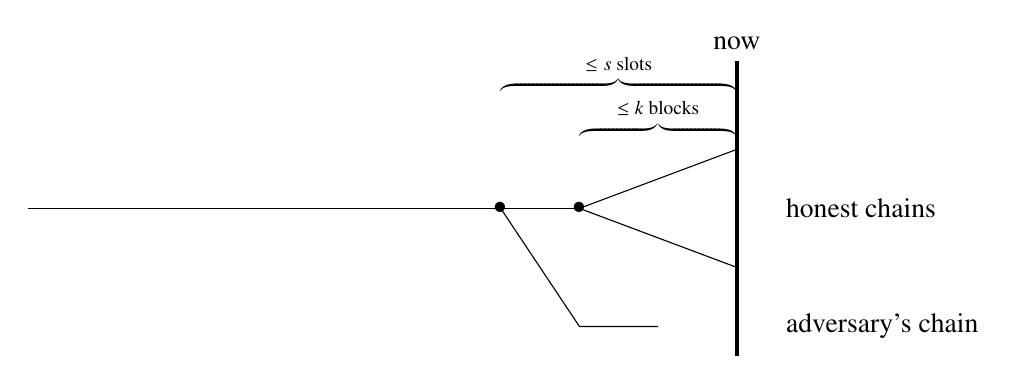
\begin{tikzpicture}[yscale=0.75]
\draw
     (0,0)
  -- (6,0) coordinate (s-back) node{$\bullet$}
  -- (7,0) coordinate (k-back) node{$\bullet$};
\draw
     (k-back)
  -- ++(2, 1)
  -- ++(0, -2) node[pos=0.5,right=0.5]{honest chains}
  -- cycle;
\draw
     (s-back)
  -- ++(1, -2)
  -- ++(1, 0) node[right=1.5cm]{adversary's chain};
\path
     (k-back)
  -- ++(0, 1)
  -- ++(2, 0) node[pos=0.5,above]{$\overbrace{\hspace{2cm}}^{\text{$\le k$ blocks}}$};
\path
     (s-back)
  -- ++(0, 1.75)
  -- ++(3, 0) node[pos=0.5,above]{$\overbrace{\hspace{3cm}}^{\text{$\le s$ slots}}$};
\draw [very thick] (9, -2.5) -- (9, 2.5) node[above]{now};
\end{tikzpicture}
\end{center}
%
The intersection between the alert node's chain and the adversarial chain is
within $s$ slots from the wallclock. This means that density at the intersection
point is just chain length (\cref{lemma:tip-density-is-chain-length}), and
hence the property follows from \cref{lemma:adversarial-before-k}.
\end{proof}

\subsection{The original genesis rule}
\label{genesis:original}

The Density rule is simplification of the rule as presented in the paper
\cite{cryptoeprint:2018:378}.  The original rule is shown in
\cref{genesis:maxvalid-bg}, and paraphrased below:

\begin{definition}[Genesis chain selection rule, original version]
\label{genesis:originalrule}
A candidate chain is preferred over our current chain if

\begin{itemize}
\item The intersection between the candidate chain and our chain is \textbf{no
more than $k$} blocks back, and the candidate chain is strictly \textbf{longer}
than our chain.

\item If the intersection \emph{is} \textbf{more than $k$} blocks back, and the
candidate chain is \textbf{denser} (contains more blocks) than our chain in
a region of $s$ slots starting at the intersection.
\end{itemize}
\end{definition}

As we saw in \cref{lemma:rule-equivalence}, the Density rule is equivalent
to the Longest Chain rule if the intersection is within $k$ blocks, so the
original rule and the simplified form are in fact equivalent.

For completeness sake, we should note that this equivalence only holds for
suitable choice of $s$. If $s$ is much smaller (for example, the paper uses $s =
\frac{1}{4}(k/f)$ in some places), then we might have a situation such as the
following, where we have two chains $A$ and $B$; $A$ is denser than $B$ at the
intersection with $B$, but $B$ is longer:
%
\begin{center}
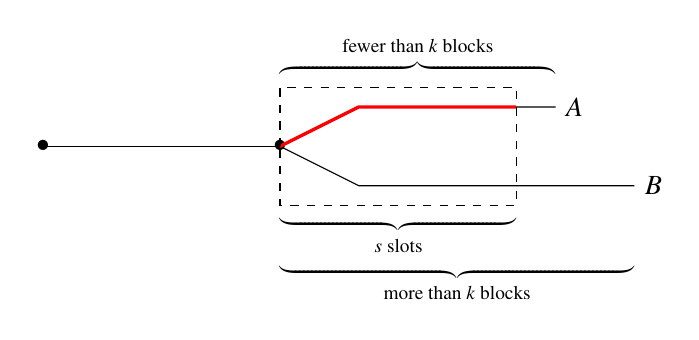
\begin{tikzpicture}
\path (0, 0) coordinate (tip) node{$\bullet$};
\draw (tip) -- ++(1.0,  0.5) -- ++(2.5, 0) coordinate(C1) node[right]{$A$};
\draw (tip) -- ++(1.0, -0.5) -- ++(3.5, 0) coordinate(C2) node[right]{$B$};
\draw [red, very thick] (tip) -- ++(1.0,  0.5) -- ++(2.0, 0);
\draw [dashed]
     (tip)
  -- ++(0, 0.75)
  -- ++(3, 0)
  -- ++(0, -1.5)
  -- ++(-3, 0) node[pos=0.5, below]{$\underbrace{\hspace{3cm}}_{\text{$s$ slots}}$}
  -- cycle;
\path (tip) -- (C1) node[pos=0.5, above=0.5cm]{$\overbrace{\hspace{3.5cm}}^{\text{fewer than $k$ blocks}}$};
\path (tip) -- (C2) node[pos=0.5, below=1.1cm]{$\underbrace{\hspace{4.5cm}}_{\text{more than $k$ blocks}}$};
\draw (tip) + (-3,0) node{$\bullet$} -- (tip);
\end{tikzpicture}
\end{center}
%
In this case, the original rule ends up preferring either $A$ or $B$ depending
on the order in which we consider them, whereas the Density Rule would simply
pick $A$.

\begin{figure}
\hrule

\textbf{Parameters} \\[0.5em]
\begin{tabular}{ll}
$C_\mathit{loc}$ & Current chain \\
$\mathcal{N} = \{C_1, \ldots, C_M\}$ & All possible chains (including our own) \\
$k$ & Security parameter (\cref{consensus:overview:k}) \\
$s$ & Genesis window size (Genesis rule specific parameter) \\
$f$ & Active slot coefficient (\cref{praos:f}) \\[1em]
\end{tabular}

\textbf{Algorithm}

\begin{lstlisting}[escapeinside={(*}{*)}, language={}, keywords={for,do,if,then,else,end,return}]
// Compare (*$C_\mathit{max}$*) to each (*$C_i \in \mathcal{N}$*)
Set (*$C_\mathit{max} \leftarrow C_\mathit{loc}$*)
for (*$i = 1$*) to (*$M$*) do
  if (*$(C_i \text{ forks from } C_\mathit{max} \text{ at most } k \text{ blocks})$*) then
    if (*$|C_i| > |C_\mathit{max}|$*) then // Condition A
      Set (*$C_\mathit{max} \leftarrow C_i$*).
  else
    Let (*$j \leftarrow \max \Bigl\{ j' \ge 0 \mathrel{\Bigl\lvert} C_\mathit{max} \text{ and } C_i \text{ have the same block in } \mathtt{sl}_{j'} \Bigr\} $*)
    if (*$|C_i[0 : j + s]| > |C_\mathit{max}[0 : j + s]|$*) then // Condition B
      Set (*$C_\mathit{max} \leftarrow C_i$*).
return (*$C_\mathit{max}$*)
\end{lstlisting}

\hrule
\caption{\label{genesis:maxvalid-bg}Algorithm \texttt{maxvalid-bg}}
\end{figure}

\section{Fragment selection}
\label{genesis:fragment-selection}

While the algorithms described in the literature on Ouroboros compare entire
chains, we will want to compare \emph{fragments} of chains: if at all possible
we would prefer not to have to download and verify entire chains before we can
make any decisions. As we have discussed in
\cref{genesis:background:joining-late}, comparing fragments (prefixes) of chains
using the Longest Chain rule does not actually make much sense, but in this
section we will see that the situation is fortunately much better when we use
the Density rule.

\begin{definition}[Preferred fragment]
Let $\mathcal{S}$ be set of chain fragments, all anchored at the same point
(that is, the fragments share a common ancestor), corresponding to some set of
chains $\mathcal{C}$. Then $A$ is a preferred fragment in $\mathcal{S}$ if and
only if $A$ is a fragment of a preferred chain in $\mathcal{C}$.
\end{definition}

We will now establish the (necessary and sufficient) condition for fragment
preference to be decidable. First, if we have to choose between two chains, we
must see enough of those chains to do a density comparison.

\begin{definition}[Known density]
We say that a chain fragment has a \emph{known density} at some point $p$
if either of the following conditions hold:

\begin{enumerate}
\item The fragment contains a block after at least $s$ slots:
\begin{center}
\begin{tikzpicture}[yscale=0.75]
\path (0,0) -- (9,0); % adjust bounding box
\path (0,0) -- (1,0) node[pos=0.5]{$\cdots$};
\draw
     (1,0)
  -- (3,0)   node{$\bullet$} node[above left]{$p$} coordinate(p)
  -- (3.5,0) node{$\bullet$}
  -- (4,0);
\path
     (4,0)
  -- (5,0) node[pos=0.5]{$\cdots$};
\draw
     (5,0)
  -- (5,0) node{$\bullet$}
  -- (6,0) node{$\bullet$}
  -- (7,0) node[red]{$\bullet$}
  -- (8,0) node[right]{$\cdots$};
\draw [dashed]
     (p)
  -- ++(0, 1)
  -- ++(3.5, 0) node[pos=0.5,above]{$s$ slots}
  -- ++(0, -2)
  -- ++(-3.5, 0)
  -- cycle;
\end{tikzpicture}
\end{center}

\item The chain (not just the fragment\footnote{We can distinguish between these
two cases because nodes report the tip of their chain as part of the chain sync
protocol, independent from the headers that we have downloaded from those
nodes.}) terminates within the window:
\begin{center}
\begin{tikzpicture}[yscale=0.75]
\path (0,0) -- (9,0); % adjust bounding box
\path (0,0) -- (1,0) node[pos=0.5]{$\cdots$};
\draw
     (1,0)
  -- (3,0)   node{$\bullet$} node[above left]{$p$} coordinate(p)
  -- (3.5,0) node{$\bullet$}
  -- (4,0);
\path
     (4,0)
  -- (5,0) node[pos=0.5]{$\cdots$};
\draw
     (5,0)
  -- (6,0) node[red]{$\bullet$};
\draw [dashed]
     (p)
  -- ++(0, 1)
  -- ++(3.5, 0) node[pos=0.5,above]{$s$ slots}
  -- ++(0, -2)
  -- ++(-3.5, 0)
  -- cycle;
\end{tikzpicture}
\end{center}
\end{enumerate}
\end{definition}

\begin{definition}[Look-ahead closure]
\label{lookahead-closure}
Let $\mathcal{S}$ be a set of chain fragments all anchored at the same point. We
say that $\mathcal{S}$ is \emph{look-ahead closed} if whenever there are two
fragments $A, B \in \mathcal{S}$, the densities of $A$ and $B$ are known at
their intersection.
\end{definition}

\begin{lemma}[Look-ahead closure is sufficient for fragment selection]
\label{lemma:fragment-selection}
Let $\mathcal{S}$ be a look-ahead closed set of chain fragments. Then
we can always choose a preferred fragment in $\mathcal{S}$.
\end{lemma}

\begin{proof}[Proof (sketch)]
In order to be able to pick a chain, we need to resolve forks. In order to
resolve forks using the Density Rule, we need to know the density, but that
is precisely what is guaranteed by look-ahead closure.
\end{proof}

\Cref{lemma:fragment-selection} is relevant because it reflects how the
consensus layer uses chain selection:

\begin{enumerate}
\item We maintain a fragment of the chain for each upstream peer we track
(\cref{chainsyncclient}). The block fetch client
(\cref{chainsyncclient:plausiblecandidates}) then picks a preferred fragment and
downloads that.
\item When the chain database needs to construct the current chain
(\cref{chainsel}), it constructs a set of chain fragments through the volatile
DB, all anchored at the tip of the immutable database, picks a preferred
fragment, and adopts that as the node's current chain.
\end{enumerate}

However, \cref{lemma:fragment-selection} is less useful than it might seem:
the look-ahead closure requirement means that in the worst case, we still need
to see entire chains before we can make a decision: every new intersection point
requires us to see $s$ more slots:
%
\begin{center}
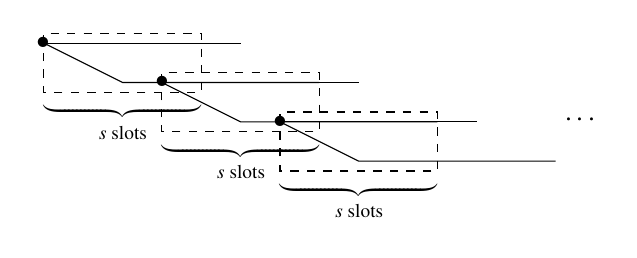
\begin{tikzpicture}[yscale=0.5]
\path (0,0) coordinate(I);
%
\node at (I) {$\bullet$};
\draw (I) -- ++(2.5, 0);
\draw (I) -- ++(1,-1) -- ++(0.5,0) coordinate(A) -- ++(2,0);
\draw [dashed]
     (I)
  -- ++(0,0.25)
  -- ++(2,0)
  -- ++(0,-1.5)
  -- ++(-2,0) node[pos=0.5,below]{$\underbrace{\hspace{2cm}}_\text{$s$ slots}$}
  -- cycle;
%
\node at (A) {$\bullet$};
\draw (A) -- ++(2.5, 0);
\draw (A) -- ++(1,-1) -- ++(0.5,0) coordinate(B) -- ++(2,0);
\draw [dashed]
     (A)
  -- ++(0,0.25)
  -- ++(2,0)
  -- ++(0,-1.5)
  -- ++(-2,0) node[pos=0.5,below]{$\underbrace{\hspace{2cm}}_\text{$s$ slots}$}
  -- cycle;
%
\node at (B) {$\bullet$};
\draw (B) -- ++(2.5, 0);
\draw (B) -- ++(1,-1) -- ++(0.5,0) coordinate(C) -- ++(2,0) node[above=0.5cm, right]{$\cdots$};
\draw [dashed]
     (B)
  -- ++(0,0.25)
  -- ++(2,0)
  -- ++(0,-1.5)
  -- ++(-2,0) node[pos=0.5,below]{$\underbrace{\hspace{2cm}}_\text{$s$ slots}$}
  -- cycle;
\end{tikzpicture}
\end{center}
%
Moreover, due to the header/body split
(\cref{nonfunctional:network:headerbody}), when we are tracking the headers from
an upstream peer, we cannot (easily) verify headers that are more than $3k/f$
slots away from the intersection between our chain and their chain (see also
\cref{low-density}). In the next section we will therefore consider how we can
drop the look-ahead closure requirement.

In case it is not obvious why we must only compare density at intersection
points, in the remainder of this section we will consider an example that will
hopefully clarify it. Suppose a malicious node with some stake intentionally
skips their slot, after which the chain continues to grow as normal:
%
\begin{center}
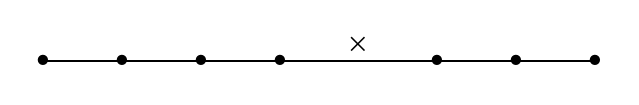
\begin{tikzpicture}
\draw
       (0,0) node{$\bullet$}
  -- ++(1,0) node{$\bullet$}
  -- ++(1,0) node{$\bullet$}
  -- ++(1,0) node{$\bullet$}
  -- ++(1,0) node[above]{$\times$}
  -- ++(1,0) node{$\bullet$}
  -- ++(1,0) node{$\bullet$}
  -- ++(1,0) node{$\bullet$};
\end{tikzpicture}
\end{center}
%
It is now trivial for the adversary to create an alternative chain that
\emph{does} have a block in that slot; if other nodes switch to the denser chain
the moment they see a window of $s$ slots that is denser, they would adopt the
adversary's chain; after all, it has one more block in the window than the
honest chain does:
%
\begin{center}
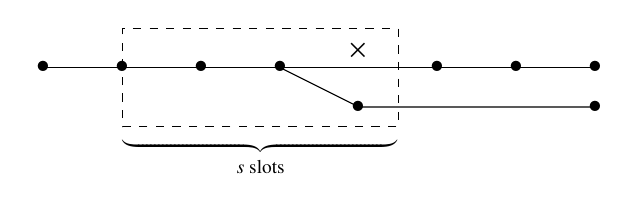
\begin{tikzpicture}[yscale=0.5]
\draw
       (0,0) node{$\bullet$}
  -- ++(1,0) node{$\bullet$} coordinate(s-anchor)
  -- ++(1,0) node{$\bullet$}
  -- ++(1,0) node{$\bullet$} coordinate(branch)
  -- ++(1,0) node[above]{$\times$}
  -- ++(1,0) node{$\bullet$}
  -- ++(1,0) node{$\bullet$}
  -- ++(1,0) node{$\bullet$};
\draw
       (branch)
  -- ++(1, -1) node{$\bullet$}
  -- ++(3,  0) node{$\bullet$};
\draw [dashed]
     (s-anchor)
  -- ++(0,1)
  -- ++(3.5,0)
  -- ++(0,-2.5)
  -- ++(-3.5,0) node[below, pos=0.5]{$\underbrace{\hspace{3.5cm}}_{\text{$s$ slots}}$}
  -- cycle;
\end{tikzpicture}
\end{center}
%
Instead, we must wait until we make such a comparison until we have reached
the intersection point:
%
\begin{center}
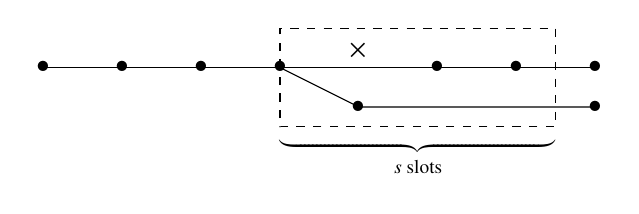
\begin{tikzpicture}[yscale=0.5]
\draw
       (0,0) node{$\bullet$}
  -- ++(1,0) node{$\bullet$}
  -- ++(1,0) node{$\bullet$}
  -- ++(1,0) node{$\bullet$} coordinate(branch)
  -- ++(1,0) node[above]{$\times$}
  -- ++(1,0) node{$\bullet$}
  -- ++(1,0) node{$\bullet$}
  -- ++(1,0) node{$\bullet$};
\draw
       (branch)
  -- ++(1, -1) node{$\bullet$}
  -- ++(3,  0) node{$\bullet$};
\draw [dashed]
     (branch)
  -- ++(0,1)
  -- ++(3.5,0)
  -- ++(0,-2.5)
  -- ++(-3.5,0) node[below, pos=0.5]{$\underbrace{\hspace{3.5cm}}_{\text{$s$ slots}}$}
  -- cycle;
\end{tikzpicture}
\end{center}
%
Since the adversary does not have sufficient stake, their chain will be less
dense and we will therefore not select it. If the adversary creates another fork
earlier on the chain, then we will resolve that fork when we encounter it using
a window of $s$ slots \emph{anchored at that fork}, and then later resolve the
second fork using a \emph{different} window of $s$ slots, anchored at the second
fork:
%
\begin{center}
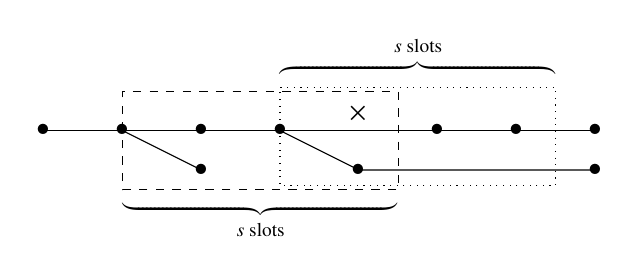
\begin{tikzpicture}[yscale=0.5]
\draw
       (0,0) node{$\bullet$}
  -- ++(1,0) node{$\bullet$} coordinate(s-anchor)
  -- ++(1,0) node{$\bullet$}
  -- ++(1,0) node{$\bullet$} coordinate(branch)
  -- ++(1,0) node[above]{$\times$}
  -- ++(1,0) node{$\bullet$}
  -- ++(1,0) node{$\bullet$}
  -- ++(1,0) node{$\bullet$};
\draw
       (branch)
  -- ++(1, -1) node{$\bullet$}
  -- ++(3,  0) node{$\bullet$};
\draw
       (s-anchor)
  -- ++(1, -1) node{$\bullet$};
\draw [dashed]
     (s-anchor)
  -- ++(0,1)
  -- ++(3.5,0)
  -- ++(0,-2.5)
  -- ++(-3.5,0) node[below, pos=0.5]{$\underbrace{\hspace{3.5cm}}_{\text{$s$ slots}}$}
  -- cycle;
\draw [dotted]
     (branch) ++ (0, 0.1)
  -- ++(0,1)
  -- ++(3.5,0)  node[above, pos=0.5]{$\overbrace{\hspace{3.5cm}}^{\text{$s$ slots}}$}
  -- ++(0,-2.5)
  -- ++(-3.5,0)
  -- cycle;
\end{tikzpicture}
\end{center}

\pagebreak

\section{Prefix selection}
\label{genesis:prefix-selection}

\subsection{Preferred prefix}

When a set $\mathcal{S}$ of chain fragments is not look-ahead closed, we may
not be able to pick a best fragment. For example, in
%
\begin{equation*}
\mathcal{S} = \left\{ \;
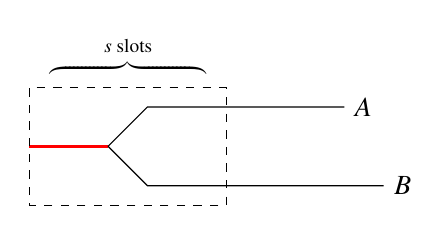
\begin{tikzpicture}[baseline=0pt, xscale=0.5,yscale=0.5]
\draw [very thick, red] (-2,0) -- (0,0);
\draw (0,0) -- (1, 1) -- (6,  1) node[right]{$A$};
\draw (0,0) -- (1,-1) -- (7, -1) node[right]{$B$};
\draw [dashed] (-2,0) -- ++(0,1.5) -- ++(5,0) node[pos=0.5,above]{$\overbrace{\hspace{2cm}}^\text{$s$ slots}$} -- ++(0,-3) -- ++(-5,0) -- cycle;
\end{tikzpicture}
\right\}
\end{equation*}
%
we cannot choose between $A$ and $B$; what we \emph{can} say however is that no
matter which of $A$ and $B$ turns out to be the better fragment, the common
prefix of $A$ and $B$ (shown in red) will definitely be a prefix of that
fragment. This example provides the intuition for the definition of a preferred
prefix:

\begin{definition}[Preferred prefix]
Given a set $\mathcal{S}$ of chain fragments, all anchored at the same point, a
preferred prefix is a prefix $\Pi$ of one of the fragments in $\mathcal{S}$,
such that $\Pi$ is guaranteed to be a prefix of a preferred fragment in the
lookahead-closure of $\mathcal{S}$.
\end{definition}

In other words, we may not be able to pick the best fragment out of
$\mathcal{S}$, but we \emph{can} pick a prefix which is guaranteed to be a
prefix of whatever turns out to be the best fragment. Obviously, the empty
fragment is always a valid choice, albeit not a particularly helpful one.
Ideally, we would choose the \emph{longest} preferred prefix. Fortunately,
constructing such a prefix is not difficult.

\subsection{Algorithm}

We will now consider how we can choose the longest preferred prefix.

\begin{definition}[Prefix selection]
\label{prefix-selection}
Let $\mathcal{S}$ be a set of chain fragments all anchored at the same point $a$,
such that all fragments have known density at point $a$. Then we can construct
the longest preferred prefix in two steps:
%
\begin{enumerate}
\item \emph{Resolve initial fork.}
Suppose $\mathcal{S}$ looks like this:
%
\begin{center}
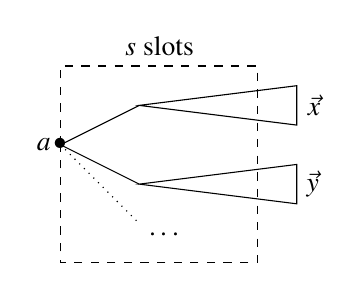
\begin{tikzpicture}
\node at (0,0) [left] {$a$};
\node at (0,0) {$\bullet$};
%
\draw (0,0) -- (1, 0.5) coordinate(x);
\draw (0,0) -- (1,-0.5) coordinate(y);
\draw [dotted] (0,0) -- (1,-1) node[below right]{$\cdots$};
%
\draw (x) -- ++(2,  0.25) -- ++(0, -0.5) node[pos=0.5,right]{$\vec{x}$} -- cycle;
\draw (y) -- ++(2,  0.25) -- ++(0, -0.5) node[pos=0.5,right]{$\vec{y}$} -- cycle;
%
\draw [dashed]
     (0,0)
  -- ++(0, 1)
  -- ++(2.5, 0) node[pos=0.5,above]{$s$ slots}
  -- ++(0, -2.5)
  -- ++(-2.5, 0)
  -- cycle;
\end{tikzpicture}
\end{center}
%
where (without loss of generality) the common prefixes are non-empty. Suppose
one of the $\vec{x}$ has the highest density\footnote{ If two fragments in
different forks have  have exactly the same density, we need a tie-breaker in
order to be able to make progress. The genesis paper does not prefer either
chain in such a scenario, switching only if another chain is strictly denser. We
can therefore follow suit, and just focus on one of the two chains arbitrarily.}
at point $a$; let's call it $x_i$. That means if we ever were to adopt any of
the $\vec{y}, \ldots$, and then compared our chain to $x_i$, we would find that
$x_i$ is denser at the intersection point (which is precisely what we are
comparing in this window here), and therefore switch to it. This means we can
focus our attention on the $\vec{x}$. (\Cref{greedy-chain-selection}
justifies the greedy nature of this algorithm in a bit more depth.)

\item \emph{Adopt common prefix.}
Most of the time, the density of the $\vec{x}$ will yet not be known at point
$b$. This means we do not yet know which $x_i$ will turn out to be the best, but
we \emph{do} know that whichever it turns out to be, it will have the common
prefix from $a$ to $b$, so we choose this as the longest preferred prefix:

\begin{center}
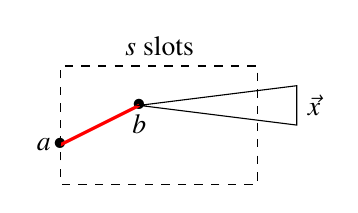
\begin{tikzpicture}
\path (0,0)   node{$\bullet$} node[left]{$a$};
\path (1,0.5) node{$\bullet$} node[below]{$b$};
%
\draw [very thick, red] (0,0) -- (1, 0.5) coordinate(x);
%
\draw (x) -- ++(2,  0.25) -- ++(0, -0.5) node[pos=0.5,right]{$\vec{x}$} -- cycle;
%
\draw [dashed]
     (0,0)
  -- ++(0, 1)
  -- ++(2.5, 0) node[pos=0.5,above]{$s$ slots}
  -- ++(0, -1.5)
  -- ++(-2.5, 0)
  -- cycle;
\end{tikzpicture}
\end{center}
%
One useful special case is when all of the $\vec{x}$ terminate within the
window. In this case, their density \emph{is} known, and we can just pick the
densest fragment as the preferred prefix; the preferred prefix is then in fact
the preferred fragment.
\end{enumerate}
\end{definition}

Prefix selection fits very naturally with the needs of the consensus layer
(\emph{cf.} the description of how consensus uses fragment selection in
\cref{genesis:fragment-selection}):
%
\begin{enumerate}
\item When blockfetch applies prefix selection to the set of fragments of
the upstream peers we are tracking, the computed prefix is precisely the set
of blocks that blockfetch should download.
\item When the chain database applies prefix selection to the set of fragments
through the volatile database, the computed prefix is precisely the chain that
we should adopt as the node's current chain.
\end{enumerate}

\begin{lemma}
If the intersection point between the chains of our upstream peers is at most
$k$ blocks away from their tips, prefix selection will choose the longest chain.
\end{lemma}

\begin{proof}[Proof (sketch)]
The proof is very similar to the proof of \cref{lemma:rule-equivalence}.
If the intersection is at most $k$ blocks away, it will be less than $s$ slots
away; therefore prefix selection will be able to see the chains to their tip,
the density of all chains will be known, and the densest fragment equals the
longest one.
\end{proof}

\begin{figure}[p]
\hrule
\vspace{0.5em}

Step 1 in \cref{prefix-selection} makes greedy decisions, discarding the less
dense chains at every step without looking further ahead. To justify this, it is
instructive to consider an apparent counter-example to the validity of this
strategy. Consider three chains $A, B, C$ in the following example:
%
\begin{center}
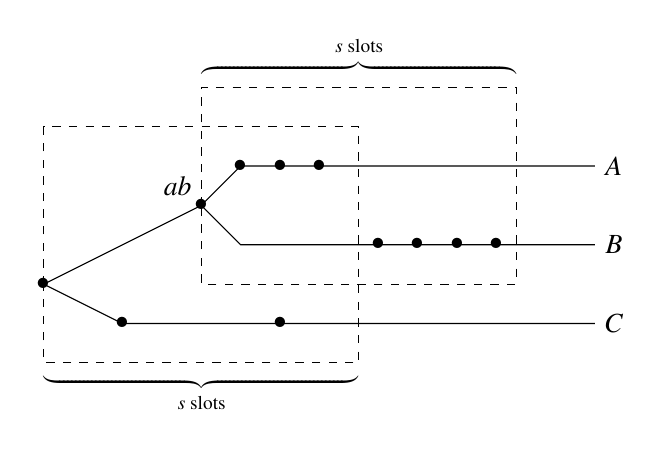
\begin{tikzpicture}
\draw
     (0, 0) node {$\bullet$} coordinate (a)
  -- (2, 1) node {$\bullet$} coordinate (b) node[above left]{$ab$};
\draw
     (a)
  -- ++(1, -0.5) node {$\bullet$}
  -- ++(2,  0  ) node {$\bullet$}
  -- ++(4,  0  ) node[right]{$C$};
\draw
     (b)
  -- ++(0.5, 0.5) node {$\bullet$}
  -- ++(0.5, 0  ) node {$\bullet$}
  -- ++(0.5, 0  ) node {$\bullet$}
  -- ++(3.5, 0  ) node[right]{$A$};
\draw
     (b)
  -- ++(0.5 , -0.5)
  -- ++(1.25,  0  )
  -- ++(0.5 ,  0  ) node {$\bullet$}
  -- ++(0.5 ,  0  ) node {$\bullet$}
  -- ++(0.5 ,  0  ) node {$\bullet$}
  -- ++(0.5 ,  0  ) node {$\bullet$}
  -- ++(1.25,  0  ) node[right]{$B$};
%
\draw [dashed]
     (a)
  -- ++(0, 2)
  -- ++(4, 0)
  -- ++(0, -3)
  -- ++(-4, 0) node[pos=0.5,below]{$\underbrace{\hspace{4cm}}_\text{$s$ slots}$}
  -- cycle;
\draw [dashed]
     (b)
  -- ++(0, 1.5)
  -- ++(4, 0) node[pos=0.5,above]{$\overbrace{\hspace{4cm}}^\text{$s$ slots}$}
  -- ++(0, -2.5)
  -- ++(-4, 0)
  -- cycle;
\end{tikzpicture}
\end{center}
%
Depending on the order in which we consider the chains, we might pick any of
these three chains:
%
\begin{center}
\begin{tabular}{l|l}
\textbf{order} & \textbf{selected chain} \\ \hline
$B, C, A$ & $A$ \\
$C, A, B$ & $B$ \\
$A, B, C$ & $C$ \\
\end{tabular}
\end{center}
%
In practice this situation cannot occur, however. The Genesis analysis tells us
that there will be single chain (the honest chain) which will be denser than any
other chain (within the genesis window) at every intersection point. This is
precisely what justifies the greedy nature of the algorithm: it will always hone
in on the honest chain. In the counter-example above, there is no single chain
with this property, and hence cannot arise.
\caption{\label{greedy-chain-selection}Greedy chain selection}
\end{figure}

\subsection{Prefix selection on headers}

When the chain sync client is deciding which of the chains of its upstream peers
to download, it does so based on chains of \emph{headers}. It does not download
block bodies and so cannot verify them. As such, it is basing its decisions
based on header validity \emph{only}.  However, this is then only used to tell
the block fetch client which blocks to \emph{download}
(\cref{chainsyncclient:plausiblecandidates}); it does not necessarily mean that
those blocks will be \emph{adopted}. When the chain database performs chain
selection (\cref{chainsel}), it will verify the blocks and discard any that turn
out to be invalid. If any blocks \emph{are} invalid, then the chain sync client
will disconnect from the nodes that provided them, which in turn may change
which prefix is chosen by prefix selection.

Indeed, the only reason to even validate headers at all is to avoid a denial
of service attack where an adversary might cause us to waste resources.
It may be worth reconsidering this risk, and balancing it against the costs
for the implementation; the only reason we need forecasting, and a special
treatment of low density chains (\cref{low-density}) is that we insist we want
to validate headers independent from blocks.

\pagebreak
\subsection{Known density}

\Cref{prefix-selection} requires known density at the anchor $a$ of the set, so
that it can resolve the initial fork. This means we have to wait until
we have downloaded enough headers from each peer: the last header we downloaded
must either be outside the $s$ window, or else it must be the last header on that
peer's chain (in which case the peer will tell us so). If a peer tells us they have
more headers but then do not provide them, we should disconnect from them
after some time-out to avoid a potential denial of service attack.

If that header is outside the genesis window, we may not be able to validate it:
since it is more than $s$ slots away from the anchor point (and we only have a
ledger state at the anchor point), it falls outside the ledger's forecast range.
However, this does not matter: the presence of this header only tells us that we
have seen everything we need to see to compute the density within the window; an
invalid header after that window cannot increase the density \emph{within} the
window.

We can make one useful exception to the known density requirement:
if there \emph{is} no initial fork, we do not need to know the density at
all and can go straight to step (2). This will allow a node to sync faster:
consider a new node that is joining the network. In most cases, all of the
node's upstream peers will report the \emph{same} blocks for all but the last
few blocks on the chain. Since there is no fork to resolve, we can start
adopting each block the moment it is reported by all peers.

\subsection{Propagation delays}

Propagation delays will be a bit slower than before. To see why, let's consider
the most ideal situation where all nodes are on exactly the same chain, and
the next slot leader produces a new block. Let
%
\begin{center}
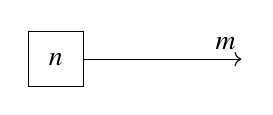
\begin{tikzpicture}[block/.style={rectangle,draw=black,minimum size=7mm}]
\node at (0,0) (A) [block] {$n$};
\draw [->] (A.east) -- ++(2,0) node[pos=0.9,above]{$m$};
\end{tikzpicture}
\end{center}
%
denote an upstream peer and a downstream peer. The upstream peer's tip is $n$,
and is sending headers to the downstream peer; the most recent header that the
downstream peer validated is $m$. When $n = m$, the downstream peer has ``seen''
the upstream peer's entire chain; in the terminology of this chapter, the
density of the upstream peer is then \emph{known}.

Consider a diamond topology with four peers $A \ldots D$, nodes $B$ and $C$
following node $A$, and node $D$ following nodes $B$ and $C$; suppose all nodes
are up to date:

\begin{center}
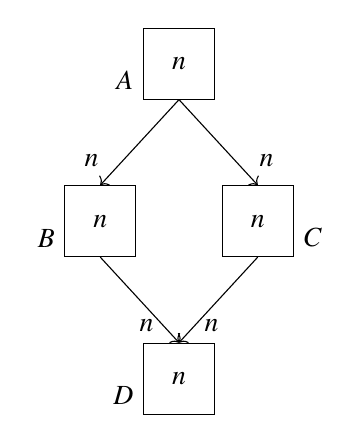
\begin{tikzpicture}[block/.style={rectangle,draw=black,minimum size=9mm}]
\node at ( 0,  0) (A) [block] {$n$};
\node at (-1, -2) (B) [block] {$n$};
\node at ( 1, -2) (C) [block] {$n$};
\node at ( 0, -4) (D) [block] {$n$};
\node at (A.south west) [above left] {$A$};
\node at (B.south west) [above left] {$B$};
\node at (C.south east) [above right] {$C$};
\node at (D.south west) [above left] {$D$};
\draw [->] (A.south) -- (B.north) node[pos=0.9,above left]{$n$};
\draw [->] (A.south) -- (C.north) node[pos=0.9,above right]{$n$};
\draw [->] (B.south) -- (D.north) node[pos=0.8,left]{$n$};
\draw [->] (C.south) -- (D.north) node[pos=0.8,right]{$n$};
\end{tikzpicture}
\end{center}

Now consider what happens when node $A$ produces a new block:\footnote{Exact
details of the chain sync protocol may mean that this example as it  stands is
not quite possible: the only way for $D$ to become aware of $C$'s new tip is
when it receives the header. However, the point still remains; have $A$ switch
to a fork instead and repeat the reasoning.}

\begin{center}
\begin{tabular}{c@{\hspace{1cm}}c@{\hspace{1cm}}c}
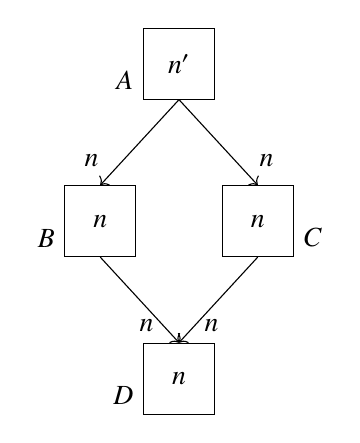
\begin{tikzpicture}[block/.style={rectangle,draw=black,minimum size=9mm}]
\node at ( 0,  0) (A) [block] {$n'$};
\node at (-1, -2) (B) [block] {$n$};
\node at ( 1, -2) (C) [block] {$n$};
\node at ( 0, -4) (D) [block] {$n$};
\node at (A.south west) [above left] {$A$};
\node at (B.south west) [above left] {$B$};
\node at (C.south east) [above right] {$C$};
\node at (D.south west) [above left] {$D$};
\draw [->] (A.south) -- (B.north) node[pos=0.9,above left]{$n$};
\draw [->] (A.south) -- (C.north) node[pos=0.9,above right]{$n$};
\draw [->] (B.south) -- (D.north) node[pos=0.8,left]{$n$};
\draw [->] (C.south) -- (D.north) node[pos=0.8,right]{$n$};
\end{tikzpicture}
&
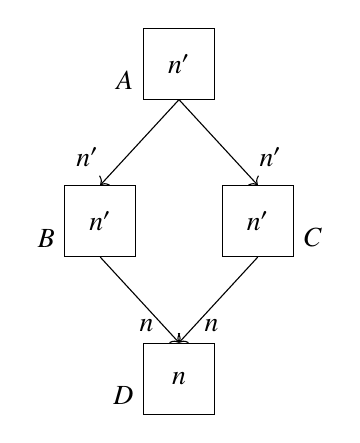
\begin{tikzpicture}[block/.style={rectangle,draw=black,minimum size=9mm}]
\node at ( 0,  0) (A) [block] {$n'$};
\node at (-1, -2) (B) [block] {$n'$};
\node at ( 1, -2) (C) [block] {$n'$};
\node at ( 0, -4) (D) [block] {$n$};
\node at (A.south west) [above left] {$A$};
\node at (B.south west) [above left] {$B$};
\node at (C.south east) [above right] {$C$};
\node at (D.south west) [above left] {$D$};
\draw [->] (A.south) -- (B.north) node[pos=0.9,above left]{$n'$};
\draw [->] (A.south) -- (C.north) node[pos=0.9,above right]{$n'$};
\draw [->] (B.south) -- (D.north) node[pos=0.8,left]{$n$};
\draw [->] (C.south) -- (D.north) node[pos=0.8,right]{$n$};
\end{tikzpicture}
&
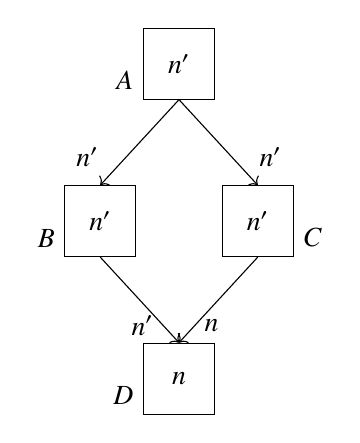
\begin{tikzpicture}[block/.style={rectangle,draw=black,minimum size=9mm}]
\node at ( 0,  0) (A) [block] {$n'$};
\node at (-1, -2) (B) [block] {$n'$};
\node at ( 1, -2) (C) [block] {$n'$};
\node at ( 0, -4) (D) [block] {$n$};
\node at (A.south west) [above left] {$A$};
\node at (B.south west) [above left] {$B$};
\node at (C.south east) [above right] {$C$};
\node at (D.south west) [above left] {$D$};
\draw [->] (A.south) -- (B.north) node[pos=0.9,above left]{$n'$};
\draw [->] (A.south) -- (C.north) node[pos=0.9,above right]{$n'$};
\draw [->] (B.south) -- (D.north) node[pos=0.8,left]{$n'$};
\draw [->] (C.south) -- (D.north) node[pos=0.8,right]{$n$};
\end{tikzpicture}
\\
(i) & (ii) & (iii)
\end{tabular}
\end{center}

Initially node $A$ announces its header to $B$ and $C$ (i), which download it
and verify it. Since their only peer is $A$, the density of ``all'' peers is now
known and so both $B$ and $C$ adopt this new block and make it available to $D$
(ii).

Suppose node $D$ now downloads that header from $B$ and verifies it (iii).
Prior to the implementation of genesis, the chain selection rule would have
concluded that this chain is longer, therefore preferred, and node $D$ would be
able to adopt the block before interacting with $C$.

Prefix selection however will \emph{wait}: it hasn't yet verified the header
from $C$, and so it considers the density of $C$'s chain's to be unknown, and
hence it cannot make a decision. \emph{This is the correct behaviour}: the
old implementation would select $C$'s chain immediately, but it would do so
for a terrible reason: sure, it's longer, but only \emph{because we downloaded
more of that chain}; this is the circular reasoning we described above in
\cref{genesis:background:joining-late}.

In principle it would be possible for $D$ to \emph{skip} the verification of
any number of headers if those headers have already been verified from another
peer. However, this would be optimising the code for the best case, with
performance degrading when the peers are on different chains; this is something
we avoid throughout (\cref{nonfunctional:best-is-worst}).







% \item When we say that the density is \emph{known}, it either means that the
% peer reports the next header to be outside the genesis window, or has given us
% the header corresponding to tip of their chain and we validated it. However,
% consider what happens when the node is up to date, and a new block is produced
% (by some other node). Strictly speaking we must now wait for \emph{all} peers to
% have provided us with this header, and have validated all those headers, before
% we would consider the density to be known and prefix selection can make progress
% (if we are up to date, all headers we receive will be within the genesis
% window). This is however unnecessary: when node $A$ provides us with a header,
% and then node $B$ reports the exact same tip, we know that node $B$'s density
% cannot exceed node $A$s, and so we can go ahead and select node $A$'s chain.
% \end{enumerate}

\section{Avoiding long rollbacks}
\label{genesis:avoiding-long-rollbacks}

\subsection{Representative sample}

At the end of \cref{genesis:background:density-rule} we mentioned that if
we have a situation such as
%
\begin{center}
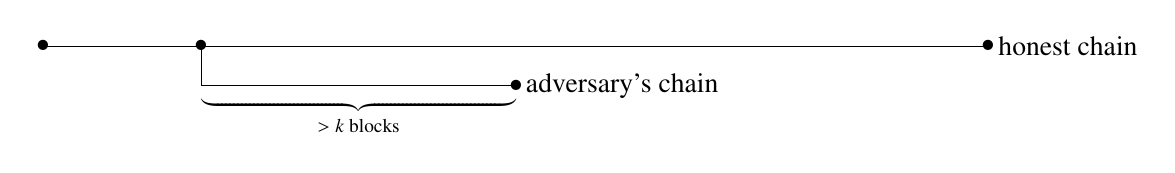
\begin{tikzpicture}[yscale=0.5]
\draw (-2,0) node{$\bullet$} -- (0,0);
\draw (0,0) node{$\bullet$} -- (10,0) node{$\bullet$} node[right] {honest chain};
\draw
     (0,0)
  -- (0,-1)
  -- (4,-1)
    node{$\bullet$}
    node[right]{adversary's chain}
    node[pos=0.5, below]{$\underbrace{\hspace{4cm}}_{\text{$> k$ blocks}}$};
\end{tikzpicture}
\end{center}
%
and we happen to adopt the adversary's chain first and later compare it to the
honest chain, the Density Rule will prefer the honest chain and so we should
switch, at the cost of a rollback of more than $k$ blocks.

Such long rollbacks are problematic; we depend on having a maximum rollback of
$k$ blocks in many ways
(\cref{consensus:overview:k,storage:components,chainsyncclient:validation,chainsyncclient:forecasting}
and others), and we will want to \emph{continue} to depend on it. However, we
needed this long rollback in this example only because we \emph{first} adopted
the adversary's chain, and \emph{then} compared it to the honest chain. In the
consensus layer even as it is today, we already don't do chain selection in such
a chain-by-chain manner; as we saw in \cref{genesis:fragment-selection} and
again in \cref{genesis:prefix-selection}, we instead pick the best out of all
currently known candidates. This means that as long as we are \emph{aware} of
both chains before we adopt either one, we will just pick the honest chain
straight away, and we avoid the rollback.

This then is the solution to avoiding longer-than-$k$ rollbacks: as long as we
are not yet up to date with the main chain, we must make sure that we connect to
a representative sample $\RequiredPeers$ of upstream peers that the probability
that \emph{none} of them will serve us the honest chain is negligible
(presumably aided by a probabilistic way of choosing upstream peers in the
network layer), and avoid doing prefix selection until we have reached
this threshold.

Of course, the need to avoid being eclipsed is not unique to genesis. When we
are up to date we can however tolerate relatively long periods in which we do
not see the honest chain; an exact analysis of the relation between the length
of such an eclipse and the maximum chain divergence we can handle is beyond the
scope of this chapter, but it seems safe to say that being eclipsed for short
periods of time should be unproblematic. If however we are behind and are
catching up with the chain, being eclipsed for even just one minute is already
problematic: an attacker can easily feed us $k$ blocks in that period, at which
point we would be unable to switch to the honest chain.

\subsection{Becoming alert}
\label{genesis:becoming-alert}

The only remaining decision to make is when we can \emph{drop} this requirement:
at which point is the state of the node comparable to the state of an alert node
(a node that has consistently been online)?

Every block that we adopt through prefix selection that is more than $s$ slots
away from the wall clock must be a block on the honest chain, because at every
fork we will only adopt blocks from the denser fragment. Moreover, all honest
parties (all alert nodes) will agree on blocks that are more than $s$ slots away
from their tip. This means that we will not need to roll back at all: any block
that we adopt which is more than $s$ slots away from the wall-clock is a block
that we can be sure about.

It is tempting to conclude from \cref{lemma:adversarial-within-s} that as soon
we have reached $s$ slots from the wallclock, we can drop the requirement to be
connected to $\RequiredPeers$ nodes and restrict rollback to  $k$ blocks. This
is however not the case. Recall what the situation looks like:
%
\begin{center}
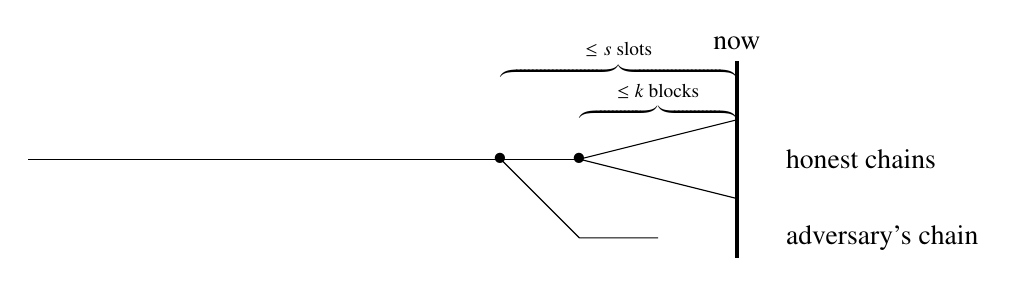
\begin{tikzpicture}[yscale=0.5]
\draw
     (0,0)
  -- (6,0) coordinate (s-back) node{$\bullet$}
  -- (7,0) coordinate (k-back) node{$\bullet$};
\draw
     (k-back)
  -- ++(2, 1)
  -- ++(0, -2) node[pos=0.5,right=0.5]{honest chains}
  -- cycle;
\draw
     (s-back)
  -- ++(1, -2)
  -- ++(1, 0) node[right=1.5cm]{adversary's chain};
\path
     (k-back)
  -- ++(0, 1)
  -- ++(2, 0) node[pos=0.5,above=-0.15]{$\overbrace{\hspace{2cm}}^{\text{$\le k$ blocks}}$};
\path
     (s-back)
  -- ++(0, 1.75)
  -- ++(3, 0) node[pos=0.5,above]{$\overbrace{\hspace{3cm}}^{\text{$\le s$ slots}}$};
\draw [very thick] (9, -2.5) -- (9, 2.5) node[above]{now};
\end{tikzpicture}
\end{center}
%
\Cref{lemma:adversarial-within-s} tells us that the adversary cannot construct a
chain that forks off more than $k$ blocks from an alert node's chain and is
longer than that chain. It does \emph{not} tell us that it cannot contain more
than $k$  blocks after the intersection.\footnote{A worst-case adversary with
near 50\% stake would be able to construct $0.5 \times 3k = 1.5k$ blocks in
$3k/f$ slots. The reasoning would be simpler if the adversary has at most 33\%
stake, as then they could indeed only construct $k$ blocks in $3k/f$ slots.}
This means that if we dropped the requirement that we see all chains and then
see and adopt the adversary's chain, we would be stuck, as switching to the
honest chain would involve a rollback of more than $k$ blocks.

\Cref{lemma:adversarial-within-s} would only help us if we are somehow
guaranteed that we have adopted one of the alert nodes' chains. But how can we
tell? Fortunately, here we have a rare example of reality serendipitously lining
up with theory. In the theoretical model, nodes collect entire chains broadcast
by their peers, and then use the density rule to select the best one. Once they
have done that, they have selected the same chain that any of the alert nodes
might have selected, and so from this point forward their state is effectively
indistinguishable from the state of an alert node.

In reality of course we cannot collect entire chains, and so we introduced
the concept of prefix selection in order to be able to apply the Density rule
incrementally. However, notice what happens when we have reached $s$ slots
from the wallclock: once we have filled our look-ahead window, \emph{we will
have seen every chain to its very tip}. Every fragment terminates within the
window, which means that prefix selection will not just pick the preferred
\emph{prefix}, and not just the preferred \emph{fragment}, but in fact the
preferred \emph{chain}. This means that just like the theory assumes, we have
selected the best chain out of all possible chains, which means we can
conclude we are now completely up to date and can resume normal operation.

\begin{definition}[Recovering ``alert'' status]
\label{recover-alert-status}
When prefix selection can see all available chains to their tip, and we have
selected and adopted the best one, the node is up to date.
\end{definition}

(TODO\todo{TODO}: Christian tells me that the genesis proof also depends on
such a ``final chain selection''. Would be good to refer to that, but I'm
not sure where that happens in the paper.)

\subsection{Avoiding DoS attacks}
\label{genesis:becoming-alert:DoS}

Malicious nodes cannot abuse \cref{recover-alert-status} in an attempt to
prevent us from concluding we are up to date: as we saw, all blocks that get us
to within $s$ slots from the wallclock come from the honest chain, and once we
have reached $s$ slots from the wallclock, an adversary cannot present us with a
chain that exceeds the window, since blocks with a slot number after the
wall-clock are invalid.

We do have to be careful if we allow for clock skew however: if a malicious node
presents us with a header past the $s$ window (and hence past the wallclock,
though within permissible skew), we would not be able to conclude that we have
become alert. This would not stop prefix selection from doing its job---after
all, a header after the window means that we now have a known density---and so
we would continue to adopt blocks from the honest chain; however, the malicious
node could keep presenting us with a header that is just out of reach,
preventing us from ever concluding we are up to date and hence from producing
new blocks. The only reason we allow for clock skew at all, however, is to avoid
branding nodes as adversarial whereas in fact its just that our clocks are
misaligned. This must therefore be a best-effort only: allow for clock skew, but
not if this would exceed $s$ slots from the intersection point.

\subsection{Falling behind}

\Cref{recover-alert-status} gives us a way to discover that we are up to date.
Deciding when we are \emph{not} up to date is less critical. One option is to
simply use the inverse of \cref{recover-alert-status} and say we are not up to
date when one of our peers provides us with a chain that we cannot see until its
tip.  Another option is to assume we are not up to date when we boot up the
node, and then only conclude that have somehow fallen behind again if we notice
that our tip is more than a certain distance away from the wallclock (at most
$s$ slots). This may need some special care; if nodes stop producing blocks for
a while, we might end up in a state in which we both conclude that we are up to
date (because we can see all of our peer's chains to their tip) and not up to
date (because our tip is too far from the wallclock). However, this scenario
needs special case anyway; we will come back to it in \cref{low-density}.

\subsection{Block production}

In principle, block production can happen even when the node is not up to date.
There is however not much point: any blocks that the node will produce while it
is not up to date are likely to be discarded almost immediately after
production, because the node will prefer the existing (honest) chain over the
tiny fork that it itself created. Moreover, blocks that we produce while we are
not up to date may in fact be helpful for an adversary. We should therefore
disable block production while the node is not up to date.

\section{Implementation concerns}

\subsection{Chain selection in the chain database}
\label{genesis:chain-database}

We mentioned in \cref{genesis:prefix-selection} that the prefix selection
interface works equally well for the chain sync client and the chain database.
They are however not doing the same thing; this is a subtle point that deserves
to be spelled out in detail.

It comes back to the difference between perceived chain length and actual chain
length (\cref{genesis:background:joining-late}). In the chain sync client this
is a meaningful and useful difference: since we are tracking chains from
individual peers, it makes sense to distinguish between having seen the tip of
that particular chain, or only seeing a prefix of that chain. However, unless we
completely change the API to the chain database, the chain database just sees
individual blocks, without knowing anything about their provenance;  it  does
therefore not know if those blocks are the tip of ``their'' chains; it's not
even clear what that would mean.

Of course, when the chain database is constructing fragments of chains through
its volatile database, it knows if a particular block is the tip of any
constructed fragment. However, that is \emph{perceived} chain length: it might
be a tip just because we haven't downloaded any more blocks yet. The difference
is important. Consider two forks like this:
%
\begin{center}
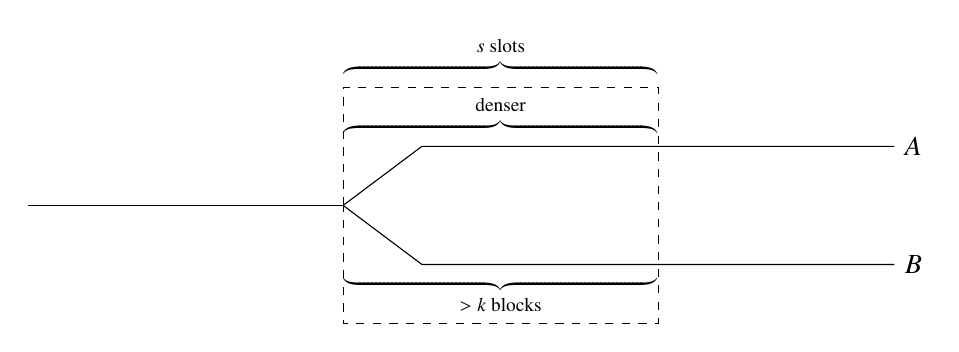
\begin{tikzpicture}[yscale=0.75]
\draw (0, 0) -- (4, 0) coordinate(i);
\draw (i) -- ++(1,  1) -- ++(6,0) node[right]{$A$};
\draw (i) -- ++(1, -1) -- ++(6,0) node[right]{$B$};
\draw [dashed]
     (i)
  -- ++( 0,  2)
  -- ++( 4,  0) node[pos=0.5,above]{$\overbrace{\hspace{4cm}}^\text{$s$ slots}$}
  -- ++( 0, -4)
  -- ++(-4,  0)
  -- cycle;
\path
     (i)
  -- ++(0, 1)
  -- ++(4, 0) node[pos=0.5,above]{$\overbrace{\hspace{4cm}}^\text{denser}$};
\path
     (i)
  -- ++(0, -1)
  -- ++(4,  0) node[pos=0.5,below]{$\underbrace{\hspace{4cm}}_\text{$> k$ blocks}$};
\end{tikzpicture}
\end{center}
%
Chain $A$ is denser in the window, but $B$ nonetheless has more than $k$ blocks
in the window (this is entirely possible; a chain of normal density would have
$3k$ blocks in the window).  The chain sync client knows about both nodes, knows
that the chains extend past the window, will wait until it has seen sufficient
blocks from both chains (that is, for the first header outside the window), then
do a density comparison, find that $A$ is denser, and choose to download the
blocks from chain $A$.

But the chain database cannot replicate any of that reasoning. When blocks  from
either chain $A$ or chain $B$ are added, as far as the chain database is
concerned, those \emph{are} the tips of those chains. This means that is not
doing a density comparison, but a chain length comparison. What's worse, if more
than $k$ blocks from chain $B$ are added before it sees any blocks from chain
$A$, then it from that point forward be unable to switch to chain $A$, as this
would involve a rollback of more than $k$ blocks.

This is not necessarily problematic: since the chain sync client has more
context, it will make the right decision, and only present blocks from chain $A$
to the database. Indeed, as we saw in \cref{genesis:becoming-alert}, we will
in fact download \emph{only} blocks from the honest chain until we are $s$
slots away from the wallclock, at which point we do one final chain selection,
and we are up to date. At this point the Density Rule is \emph{anyway} just
selecting the longest chain, so the fact that the chain database is effectively
doing longest chain selection \emph{always} does not matter.

It does however mean that the block fetch client becomes an important
``guardian'' of the chain database; they become more tightly coupled than they
are currently. This is unfortunate, but not disastrous; it ``only'' makes the
system more difficult to understand. Solving this problem would require
rethinking how the chain database works; this is well outside the scope of this
chapter.

There is one advantage to this.  \Cref{genesis:prefix-selection} describes how
the chain database could \emph{in principle} use prefix selection: compute all
paths through the volatile database and then use prefix selection to construct a
prefix that the node should adopt as its current chain. While this is a useful
\emph{specification} of what the chain database must do, in practice we will
probably need an equivalent of \cref{focusonnewblock} that will allow us to
avoid looking at the entire volatile database every time a new block is added to
the database. If we however decide that the chain database is just selecting
based on chain length \emph{anyway}, then the existing lemma and existing
implementation can be used as-is.

\subsection{Abstract chain selection interface}

The current chain selection API compares two chains at a time, and only looks at
the tips of those two chains (\cref{consensus:overview:chainsel}). This will
obviously have to change; depending on how exactly we want to modify the chain
database (\cref{genesis:chain-database}), we must either replace the existing
interface with prefix selection as the primitive operation, or else add prefix
selection as an additional concept.

One of the reasons we currently only look at the tips of chains is because this
simplified treatment of chain selection in the hard fork combinator. This by
itself might not be too difficult to change; for example, we could set the
\lstinline!SelectView! of the hard fork block to be an $n$-ary sum of the
\lstinline!SelectView!s of the various eras. However, it is not a-priori clear
what it would mean to apply, say, the Praos rule in one era on the chain,
and the Genesis rule in another. This will require some careful thought,
though we can probably just sidestep the entire issue and pretend we were
using the Genesis rule all along.

\subsection{Possible optimisations}
\label{genesis:optimisations}

Chain selection while we are not up to date has some properties that might
enable us to implement some performance optimisations. Here we just list some of
the possibilities:

\begin{itemize}

\item When a node is operational, we try to line up its average-case performance
requirements with its worst-case performance requirements, since this avoids
an attack vector: if the average-case performance would be significantly better
than the worst-case, it is likely that nodes would be optimised for the average
case (for instance, run on hardware that can handle the average case, but not
necessarily the worst case); then if a malicious node can intentionally cause
the worst-case, they might be able to bring down parts of the network.

For this reason we don't normally share work between various peers; when
multiple upstream peers all send us the same header, we verify the header
each time. This means that the average case (most upstream chains are the same)
and the worst case (every upstream chain is different) are equal.

However, it is less important that we can predict accurately how long it takes
a node (that isn't up to date) to sync with the network. Such a node is anyway
not producing blocks; here, faster is simply better. This means that while we
we are not up to date  we could share the validation work across upstream peers:
when two peers send us the same header, we do not need to validate it twice.

This is \emph{especially} important when we are not up to date, because due to
the requirement to have at least $\RequiredPeers$ upstream peers, we might be
connecting to more peers than usual. Moreover, under normal circumstances we
expect all of these peers to present us with exactly the same chain (and
finally, these cryptographic checks are expensive).

\item Similarly, since we expect all upstream nodes to report the same chain,
if we receive a bunch of headers from peer 1, we can just ask peer 2
whether they have the most recent of those headers on their chain, thereby
skipping over large chunks of the chain altogether.

\item Since we only ever fetch blocks strictly in order, we can simplify
the interaction with the block fetch client: it might be easier to generate
longer fetch ranges, as well as spread the load more evenly across the peers.

\item We saw in \cref{genesis:becoming-alert} that any blocks that we download
while syncing which are more than $s$ slots away from the wall clock, will be
blocks from the common prefix of the honest chains and will not have to be
rolled back. It might therefore be possible to bypass the volatile database
entirely. However, how this works when we switch back from being up to date
to not being up to date would require careful thought.

\end{itemize}

\chapter{Dealing with extreme low-density chains}
\label{low-density}

\section{Introduction}

As we saw in \cref{genesis}, chain density is our principal means for
distinguishing chains forged by malicious nodes from the honest chain: due to
the fundamental assumption that there is an honest majority, the chain forged by
the honest nodes will be denser than any chain forged by an adversary. If
therefore the honest nodes in the system stop producing blocks due to some
network-wide problem---pervasive node misconfiguration, bug in the ledger,
etc.---the security of the system is at risk. Even when the nodes start
producing blocks again, the low-density region of the chain left behind by the
problem will remain to be an issue for security. If an adversary forks off
their own chain at the point where the honest majority stopped producing blocks,
then new nodes joining the network (using the genesis rule, \cref{genesis}) will
adopt the adversarial chain instead of the honest chain:
%
\begin{center}
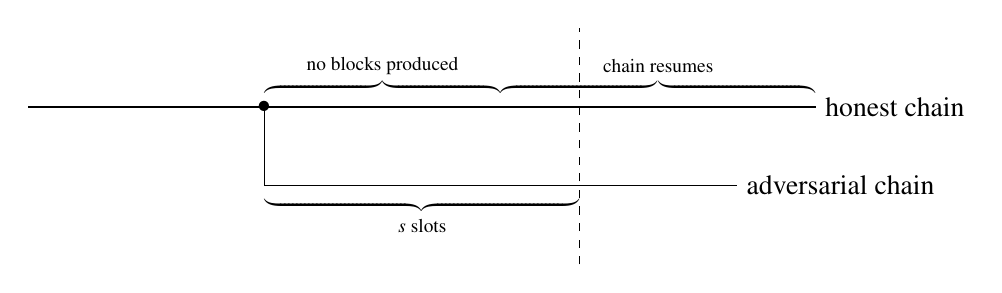
\begin{tikzpicture}
\draw
     (0,0)
  -- (3,0) node{$\bullet$} coordinate(i);
\draw
     (i)
  -- ++(3,0) node[pos=0.5,above]{$\overbrace{\hspace{3cm}}^\text{no blocks produced}$}
  -- ++(4,0) node[pos=0.5,above]{$\overbrace{\hspace{4cm}}^\text{chain resumes}$}
             node[right]{honest chain};
\draw
     (i)
  -- ++(0, -1)
  -- ++(4, 0) node[pos=0.5,below]{$\underbrace{\hspace{4cm}}_\text{$s$ slots}$}
  -- ++(2, 0) node[right]{adversarial chain};
\draw [dashed] (7,-2) -- (7,1);
\end{tikzpicture}
\end{center}
%
The \emph{Disaster Recovery Plan}\footnote{Currently not available as a public
document.} sketches how we might ``patch the chain back up'' when a major
problem like this occurs. This must happen out-of-band with the cooperation of
the major stake holders, and is (mostly) outside the scope of the Consensus
Layer report. That said, the options for disaster recovery are currently limited
due to a technical limitation in the consensus layer, which we will discuss now.

From a chain security point of view, it makes little difference if the honest
chain has a region of $s$ slots containing \emph{one} block or \emph{zero}
blocks; both are equally terrible. However, this makes a big
difference to the implementation as it currently stands: as long as there is at
least one block in every $s$ slots, the system can continue; but when there is a
gap of more than $s$ slots anywhere on the chain, the system will grind to a
halt. As we will see in this chapter, this is a consequence of the fact that we
validate headers independent from blocks, the so-called header/body split
(see also \cref{nonfunctional:network:headerbody}). The main goal of this
chapter is to discuss how we can address this, allowing the system to continue
irrespective of any gaps on the chain. This is important for a number of
reasons:

\begin{enumerate}
\item It makes disaster recovery less immediately urgent: if the honest nodes
stop producing blocks for whatever reason, the problem can be resolved, the
system restarted, and blocks can be produced again. Disaster recovery,
and patching the chain back up, can then be considered as the system is running
again, and put into motion when the various stake holders are ready.
\item It also opens up more avenues for disaster recovery. If the consensus
layer can't skip past large gaps on the chain, then the chain \emph{must} be
patched. However, if we lift this restriction, then there are other ways in
which we might address the problem. For example, we could (even if just
temporarily) simply record the low-density area of the chain within the code
itself and hardcode a preference for (this part of the) ``honest but sparse''
chain in chain selection.
\item Chain regions with extreme low density are difficult to avoid
in our consensus tests (\cref{testing:consensus}).
\end{enumerate}

Even \emph{if} it is desirable that the system stops when the chain density
falls below a certain threshold, it does not make sense to set that threshold at
the ``less than 1 block per $s$ slots'' boundary. This should be defined and
implemented as an external policy, not dictated by implementation details.
Moreover, even with an explicit stop, we might like the ability to mark the
known-to-be-low-density chain and restart the system (point 2, above). It is
also far from clear how to avoid adversarial nodes from taking advantage of such
``automatic'' stops (how do we prevent adversaries from producing blocks?).
Either way, such concerns are well outside the scope of this chapter. Here we
address just one question: how can we allow the system to continue when there
are larger-than-$s$-slots gaps on the chain.

\section{Background}

\subsection{Recap: ledger state, ledger view and forecasting}

Blocks are validated against the state of the ledger
(\cref{ledger:api:ApplyBlock}). For example, we check that inputs spent by
transactions in the block are available in the UTxO in the ledger state.
Depending on the choice of consensus protocol, we may also need part of the
ledger state to be able to validate the block \emph{header}. For example, in
Praos and Genesis we need to know the active stake distribution in order to be
able to verify that whoever produced the block had a right to do so. We call the
part of the ledger state that we need to validate block headers the \emph{ledger
view} (\cref{consensus:class:ledgerview}).

We call it a ledger \emph{view} because it is a projection out of the full
ledger state. Unfortunately, we cannot compute the \emph{next} ledger view based only
on the header; there is nothing that corresponds to the dotted arrow in this
diagram:
%
\begin{center}
\begin{tikzpicture}[block/.style={rectangle}]
\node at (0, 2) (state1) [block] {ledger state};
\node at (7, 2) (state2) [block] {ledger state};
\node at (0, 0) (view1)  [block] {ledger view};
\node at (7, 0) (view2)  [block] {ledger view};
\draw [->] (state1.south) -- (view1.north) node[pos=0.5,left]{project};
\draw [->] (state2.south) -- (view2.north) node[pos=0.5,right]{project};
\draw [->] (state1.east)  -- (state2.west) node[pos=0.5,above]{apply block};
\draw [->, dotted] (view1.east)  -- (view2.west) node[pos=0.5,below]{(cannot apply header)};
\end{tikzpicture}
\end{center}
%
Let's recall the Praos example again: we can compute the active stake
distribution from the ledger state, but in order to understand how the active
stake distribution evolves, we need to know how the full UTxO evolves, and for
that we need the full blocks. (We discussed this also in
\cref{hfc:failed:forecasting}.)

Let's stay with Praos a little longer. The active stake distribution changes
only at epoch boundaries. Therefore we will know the active stake distribution
at least until the end of the epoch.  Moreover, once we get close enough to the
epoch boundary, we also know the stake distribution for the \emph{next} epoch.
The range over which we know the active stake distribution therefore evolves as
follows:
%
\begin{center}
\begin{tikzpicture}[yscale=0.75]
%
\draw (0,  0) -- (2,  0) node{$\bullet$} node[above left]{tip};
\path (2,  0) -- (6,  0) node[pos=0.5,above]{$\overbrace{\hspace{4cm}}^\text{known}$};
%
\draw (0, -1) -- (3, -1) node{$\bullet$} node[above left]{tip};
\path (3, -1) -- (6, -1) node[pos=0.5,above]{$\overbrace{\hspace{3cm}}^\text{known}$};
%
\draw (0, -2) -- (4, -2) node{$\bullet$} node[above left]{tip};
\path (4, -2) -- (6, -2) node[pos=0.5,above]{$\overbrace{\hspace{2cm}}^\text{known}$};
%
\draw (0, -3) -- (5, -3) node{$\bullet$} node[above left]{tip};
\path (9, -3) -- (6, -3) node[pos=0.5,above]{$\overbrace{\hspace{5cm}}^\text{known}$};
%
\draw [dashed] ( 2, -3.2) -- ( 2, 0.7) node[above]{epoch};
\draw [dashed] ( 6, -3.2) -- ( 6, 0.7) node[above]{epoch};
\draw [dashed] (10, -3.2) -- (10, 0.7) node[above]{epoch};
\end{tikzpicture}
\end{center}

\pagebreak

The range over which we know the active stake distribution shrinks and then
grows again, but never falls below a certain minimum size. We abstract from this
process in the consensus layer, and say we can \emph{forecast} the ledger view
from a particular ledger state over a certain \emph{forecast range}
(\cref{ledger:api:LedgerSupportsProtocol}). This does not necessarily mean the
ledger view is constant during that range, but merely that any changes are
\emph{known} (for example, see the last line in the diagram above).

If we change our perspective slightly, we can say that blocks on the chain
cannot influence the ledger view (active stake distribution) until a certain
period of time (in slots) has passed. We call this the \emph{stability window}
of the ledger, and will study it in more detail in the next section.

\subsection{Recap: stability windows}
\label{low-density:recap-stability-window}

Blocks are validated against ledger states; each block is validated against the
ledger state as it was after applying the previous block. This means that when
we validate block $B$ in the example below, we use the ledger state after
applying block $A$; for block $C$, we use the ledger state after applying block
$B$:
%
\begin{center}
\begin{tikzpicture}
  [block/.style={rectangle,draw=black,minimum size=5mm}
  ,baseline=0pt]
\node at (0,0) (A) [block] {A};
\node at (2,0) (B) [block] {B};
\node at (5,0) (C) [block] {C};
\draw (-2,0)   -- (A.west);
\draw (A.east) -- (B.west) node[pos=0.5,above=5mm]{\small validated against};
\draw (B.east) -- (C.west) node[pos=0.5,above=5mm]{\small validated against};
\draw (C.east) -- ++(2,0);
%
\draw [->, dotted] (B.west) to [out=135,in=90] (A.east);
\draw [->, dotted] (C.west) to [out=135,in=90] (B.east);
\end{tikzpicture}
\qquad
\begin{minipage}{0.25\textwidth}
\emph{Horizontal axis represents time (in slots)}
\end{minipage}
\end{center}
%
In the chain sync client (\cref{chainsyncclient}) we are however not validating
blocks, but block \emph{headers}. As we saw, in order to validate a header we
only need part of the ledger state, known as the ledger \emph{view}. We also saw
that  despite the fact that we only need part of the ledger state, we cannot
\emph{update} the ledger view using only headers: we still need the full block.
This means that if we have block $A$, but only block \emph{headers} $B$ and $C$,
we have a problem:
%
\begin{center}
\begin{tikzpicture}
  [block/.style={rectangle,draw=black,minimum size=5mm}]
\path (-2,0) -- (11,0); % adjust bounding box
\node at (0,0) (A) [block] {A};
\node at (2,0) (B) [block, dashed] {B};
\node at (5,0) (C) [block, dashed] {C};
\draw (-2,0)   -- (A.west);
\draw (A.east) -- (B.west) node[pos=0.5,above=5mm]{\small validated against};
\draw (B.east) -- (C.west) node[pos=0.5,above=5mm]{\small validated against};
\draw (C.east) -- ++(2,0);
%
\draw [->, dotted] (B.west) to [out=135,in=90] (A.east);
\draw [->, dotted] (C.west) to [out=135,in=90] (B.east);
\end{tikzpicture}
\end{center}
%
Validating header $B$ is unproblematic, since we have the ledger state available
after applying block $A$. However, since we don't have block $B$, we can't
compute the ledger state after block $B$ to validate header $C$. We are saved by
the fact that we can \emph{forecast} the ledger view  required to validate
header $B$ from the ledger state after $A$:
%
\begin{center}
\begin{tikzpicture}
  [block/.style={rectangle,draw=black,minimum size=5mm}]
\path (-2,0) -- (11,0); % adjust bounding box
\node at (0,0) (A) [block] {A};
\node at (2,0) (B) [block, dashed] {B};
\node at (5,0) (C) [block, dashed] {C};
\draw (-2,0)   -- (A.west);
\draw (A.east) -- (B.west) node[pos=0.55,below=5mm]{\small forecast};
\draw (B.east) -- (C.west);
\draw (C.east) -- ++(2,0);
%
\draw [->, dotted] (B.west) to [out=135,in=90] (A.east);
\draw [->, dotted] (C.west) to [out=135,in=90] (B.east);
%
\draw [->, dotted] (A.east) to [out=270,in=270] (B.east);
\end{tikzpicture}
\end{center}
%
We can do this because of a restriction on the ledger: blocks cannot affect
the ledger view until a \emph{stability window} has passed:
%
\begin{center}
\begin{tikzpicture}
  [block/.style={rectangle,draw=black,minimum size=5mm}]
\path (-2,0) -- (11,0); % adjust bounding box
\node at (0,0) (A) [block] {A};
\node at (2,0) (B) [block, dashed] {B};
\node at (5,0) (C) [block, dashed] {C};
\node at (8,0) (D) [block, dashed] {D};
\draw (-2,0)   -- (A.west);
\draw (A.east) -- (B.west) node[pos=0.55,below=5mm]{\small forecast};
\draw (B.east) -- (C.west);
\draw (C.east) -- (D.west);
\draw (D.east) -- ++(2,0);
%
\draw [->, dotted] (B.west) to [out=135,in=90] (A.east);
\draw [->, dotted] (C.west) to [out=135,in=90] (B.east);
%
\draw [->, dotted] (A.east) to [out=270,in=270] (B.east);
\node at (B.east) [below=0.6, right] {$\underbrace{\hspace{4cm}}_\text{stability window}$};
\node at (7,0) {$\times$};
\end{tikzpicture}
\end{center}
%
We can use the ledger state after applying block $A$ (which we
have complete knowledge of) to validate any header up to the end of $B$'s
stability window: any changes that $A$ (or any block before $A$)
initiates we know about, and any changes that $B$ initiates cannot take effect
until that stability window ends. Therefore we can validate header $C$, but not
header $D$: block $B$ might have scheduled some changes to take effect at the
slot marked as $(\times)$ in the diagram, and we do not know what those effects
are.\footnote{It might be tempting to think that we can validate $D$ because if
we did have blocks $B$ and $C$, block $D$ would be evaluated against the ledger
state as it was after applying $C$, which is still within $B$'s stability
window. However, the slot number of $D$ (its location on the $x$-axis in the
diagram) matters, because changes are scheduled for slots.}

In chain sync we do not currently take advantage of the knowledge of the
location of header $B$.\footnote{\label{footnote:anchor-after-first-header}We
should change this. By anchoring the stability window at the last known block,
we only have a guarantee that we can validate $k$ headers, but we should really
be able to validate $k + 1$ headers in order to get a chain that is longer than
our own (\cref{low-density:tension}). If we anchored the stability window after
the first unknown header, where it \emph{should} be anchored, we can validate
$k$ headers \emph{after} the first unknown header, and hence $k + 1$ in total.
Concretely, we would have to extend the \lstinline!LedgerSupportsProtocol! class
with a function that forecasts the ledger view given a \emph{ticked} ledger
state. Taking advantage of this would then just be a minor additional
complication in the chain sync client.}  This means we have to be conservative:
all we know is that there could be \emph{some} block in between $A$ and $C$ that
might schedule some changes that are relevant for validating header $C$. In this
case we therefore assume that the stability window extends from $A$ instead:
%
\begin{center}
\begin{tikzpicture}
  [block/.style={rectangle,draw=black,minimum size=5mm}]
\path (-2,0) -- (11,0); % adjust bounding box
\node at (0,0) (A) [block] {A};
\node at (2,0) (B) [block, dashed] {B};
\node at (5,0) (C) [block, dashed] {C};
\node at (8,0) (D) [block, dashed] {D};
\draw (-2,0)   -- (A.west);
\draw (A.east) -- (B.west);
\draw (B.east) -- (C.west);
\draw (C.east) -- (D.west);
\draw (D.east) -- ++(2,0);
%
\node at (A.east) [below=0.6, right] {$\underbrace{\hspace{4cm}}_\text{stability window}$};
\end{tikzpicture}
\end{center}
%
In this example, that means we can validate $B$, but not $C$ (nor
$D$).\footnote{We could in principle shift this up by 1 slot: after all, the
very first next block after $A$ cannot be in the same slot as $A$. While EBBs
are an exception to that rule (\cref{ebbs}), we do not need to validate EBBs so
this is a rare example where EBBs do not cause a problem.}

\subsection{Tension with chain selection}
\label{low-density:tension}

Changes that affect the ledger view are scheduled for slots (often
for epoch boundaries, which happen at particular slots); the stability window
must therefore be defined in terms of slots as well. This means that
the number of \emph{headers} we can validate within a given stability window
depends on the density of that chain; if the chain we considered at the end
of the previous section looks like this instead
%
\begin{center}
\begin{tikzpicture}
  [block/.style={rectangle,draw=black,minimum size=5mm}]
\path (-2,0) -- (11,0); % adjust bounding box
\node at (0,0) (A) [block] {A};
\node at (1.5,0) (B) [block, dashed] {B};
\node at (3,0) (C) [block, dashed] {C};
\node at (8,0) (D) [block, dashed] {D};
\draw (-2,0)   -- (A.west);
\draw (A.east) -- (B.west);
\draw (B.east) -- (C.west);
\draw (C.east) -- (D.west);
\draw (D.east) -- ++(2,0);
%
\node at (A.east) [below=0.6, right] {$\underbrace{\hspace{4cm}}_\text{stability window}$};
\end{tikzpicture}
\end{center}
%
we can validate headers $B$ and $C$ (but still not $D$).

There is a fundamental tension between the stability window defined in
\emph{slots}, and chain selection preferring  longer chains: chains that have
more \emph{blocks}. In order to be able to do a meaningful comparison between
our chain and the candidate chain, we must be able to verify enough of that
candidate chain that the length of that verified prefix exceeds the length of
our own chain. Since the maximum rollback we support is $k$
(\cref{consensus:overview:k}), that means we must be able to validate at least
$k + 1$ headers. The tension is resolved by a theoretical result that says that
within $3k/f$ slots we \emph{will} see more than $k$ blocks (more precisely, the
probability that we see fewer than $k$ blocks in $3k/f$ slots is negligibly
small; \cite{cryptoeprint:2017:573}). This therefore provides us with a suitable
choice for a stability window.

Unfortunately, while in theory there is no difference between theory and
practice, there is in practice. Currently, when all nodes in the system are
unable to produce blocks for an extended period of time, the system grinds to a
halt. Even if the underlying problem is resolved, nodes will refuse to create a
block if the distance between that block and the previous block exceeds the
stability window; after all, if they did produce a block, other nodes would be
unable to validate it. The former is easily resolved, this is merely a check in
the block production code; resolving the second problem is the topic of this
chapter.

It would be preferable to avoid the tension altogether, and schedule
changes that affect the ledger view for particular \emph{blocks} instead
(and consequently, have epoch boundaries also happen at certain blocks). This
however requires backing from theoretical research; we will come back to this
in \cref{future:block-vs-slot}.

\pagebreak

\subsection{Single-gap case}

It is tempting to think that when there is only a \emph{single} large gap
on the chain, there is no problem:
%
\begin{center}
\begin{tikzpicture}
  [block/.style={rectangle,draw=black,minimum size=5mm}]
\path (-2,0) -- (11,0); % adjust bounding box
\node at (0,0) (A) [block] {A};
\node at (6,0) (B) [block, dashed] {B};
\node at (7,0) (C) [block, dashed] {C};
\node at (8,0) (D) [block, dashed] {D};
\draw (-2,0)   -- (A.west);
\draw (A.east) -- (B.west);
\draw (B.east) -- (C.west);
\draw (C.east) -- (D.west);
\draw (D.east) -- ++(2,0);
%
\node at (B.east) [below=0.6, right] {$\underbrace{\hspace{4cm}}_\text{stability window}$};
\end{tikzpicture}
\end{center}
%
The gap between $A$ and $B$ exceeds the stability window, but this
should not matter: it's not the stability window after $A$ that
matters, but the stability window after $B$. This seems to be a useful special
case: if a problem \emph{does} arise that prevents nodes from producing blocks
for an extended period of time, one might hope that this problem does not
immediately arise again after the nodes resume producing blocks.

As we saw, the consensus layer always conservatively anchors the stability
window at the last known block rather than the first header after the tip. We
could change this (and probably should; see
\cref{footnote:anchor-after-first-header}), but it turns out this does not
actually help very much for this particular problem. To see this, suppose there
is another node in the system which is currently on a fork that intersects with
this chain after some block $I$ before the gap:
%
\begin{center}
\begin{tikzpicture}[yscale=0.5,block/.style={rectangle,draw=black,minimum size=5mm}]
\node at (-2,-1) (I) [block] {I};
\node at (0,0) (A) [block, dashed] {A};
\node at (6,0) (B) [block, dashed] {B};
\node at (7,0) (C) [block, dashed] {C};
\node at (8,0) (D) [block, dashed] {D};
\draw (-4,-1)   -- (I.west);
\draw (I.east) -- (A.west);
\draw (A.east) -- (B.west);
\draw (B.east) -- (C.west);
\draw (C.east) -- (D.west);
\draw (D.east) -- ++(2,0);
%
\node at (A.east) [below=0.6, right] {$\underbrace{\hspace{4cm}}_\text{stability window}$};
%
\node at (0, -2) (A') [block] {A$'$};
\draw (I.east) -- (A'.west);
\end{tikzpicture}
\end{center}
%
The second node must execute a rollback to $I$ in order to be able to adopt
the new chain, but from \emph{its} perspective the first unknown block is $A$,
not $B$: hence the stability window \emph{must} be anchored at $A$, and the
node will be unable to bridge the gap.

\section{Pre-genesis}
\label{low-density:pre-genesis}

In this section we will consider how we might allow nodes to recover from a low
density chain, prior to the implementation of the genesis rule. An obvious
solution suggests itself: we could just allow chain sync to download blocks
when it needs to validate a header which is beyond its forecast range.

\subsection{Damage mitigation}

The reason the chain sync client doesn't normally download blocks is to limit
the amount of unnecessary work an attacker can make it do (prevent DoS attacks,
\cref{nonfunctional:network:headerbody}). We might therefore consider if we can
restrict \emph{when} we allow the chain sync client to download blocks. Ideally
we would do this only ``when necessary'': to bridge the gap on the honest chain.
Unfortunately, it is difficult to come up with a criterion that
approximates this ideal. Consider how the situation evolves from the point of
view of a single node:

\begin{center}
\begin{tikzpicture}[yscale=0.25]
%
\path (0, 0) coordinate(imm1) node{$\bullet$} node[above]{imm};
\draw (imm1) -- ++(-1,0);
\draw (imm1) -- ++(0.5,0);
\path (imm1) -- ++(0.5,0) -- ++(1,0) node[pos=0.5]{$\cdots$} -- ++(0.5,0) coordinate(cp1);
\draw (cp1) -- ++(-0.5,0);
\draw (cp1) -- ++(1, 1.5) -- ++(1,   0) node{$\bullet$};
\draw (cp1) -- ++(1, 0.5) -- ++(1.5, 0) node{$\bullet$};
\draw (cp1) -- ++(1,-0.5) -- ++(0.5, 0) node{$\bullet$};
\draw (cp1) -- ++(1,-1.5) -- ++(1,   0) node{$\bullet$};
\draw [very thick] (4.5,-2) -- (4.5,2) node[above]{now};
%
\path (0, -7) coordinate(imm2) node{$\bullet$} node[above]{imm};
\draw (imm2) -- ++(-1,0);
\draw (imm2) -- ++(0.5,0);
\path (imm2) -- ++(0.5,0) -- ++(1,0) node[pos=0.5]{$\cdots$} -- ++(0.5,0) coordinate(cp2);
\draw (cp2) -- ++(-0.5,0);
\draw (cp2) -- ++(1, 1.5) -- ++(1,   0) node{$\bullet$};
\draw (cp2) -- ++(1, 0.5) -- ++(1.5, 0) node{$\bullet$};
\draw (cp2) -- ++(1,-0.5) -- ++(0.5, 0) node{$\bullet$};
\draw (cp2) -- ++(1,-1.5) -- ++(1,   0) node{$\bullet$};
\draw [very thick] (5.5,-9) -- (5.5,-5) node[above]{now};
%
\path (0, -14) coordinate(imm3) node{$\bullet$} node[above]{imm};
\draw (imm3) -- ++(-1,0);
\draw (imm3) -- ++(0.5,0);
\path (imm3) -- ++(0.5,0) -- ++(1,0) node[pos=0.5]{$\cdots$} -- ++(0.5,0) coordinate(cp3);
\draw (cp3) -- ++(-0.5,0);
\draw (cp3) -- ++(1, 1.5) -- ++(1,   0) node{$\bullet$};
\draw (cp3) -- ++(1, 0.5) -- ++(1.5, 0) node{$\bullet$};
\draw (cp3) -- ++(1,-0.5) -- ++(0.5, 0) node{$\bullet$};
\draw (cp3) -- ++(1,-1.5) -- ++(1,   0) node{$\bullet$};
\path (4.5,-12.5) -- (7.5,-12.5) node[pos=0.5,above=-0.1]{$\overbrace{\hspace{3cm}}^\text{$> s$ slots}$};
\draw [very thick] (7.5,-16) -- (7.5,-12) node[above]{now};
%
\path (0, -21) coordinate(imm4) node{$\bullet$} node[above]{imm};
\draw (imm4) -- ++(-1,0);
\draw (imm4) -- ++(0.5,0);
\path (imm4) -- ++(0.5,0) -- ++(1,0) node[pos=0.5]{$\cdots$} -- ++(0.5,0) coordinate(cp4);
\draw (cp4) -- ++(-0.5,0);
\draw (cp4) -- ++(1, 1.5) -- ++(1,   0) node{$\bullet$} coordinate(before1);
\draw (cp4) -- ++(1, 0.5) -- ++(1.5, 0) node{$\bullet$};
\draw (cp4) -- ++(1,-0.5) -- ++(0.5, 0) node{$\bullet$} coordinate(before2);
\draw (cp4) -- ++(1,-1.5) -- ++(1,   0) node{$\bullet$};
\path (4.5,-19.5) -- (7.5,-19.5) node[pos=0.5,above=-0.1]{$\overbrace{\hspace{3cm}}^\text{$> s$ slots}$};
\draw [very thick] (10,-23) -- (10,-19) node[above]{now};
\path (before1) -- ++(5,0) coordinate(after1);
\path (before2) -- ++(6,0) coordinate(after2);
\draw (after1) node{$\bullet$} -- ++(2,0);
\draw (after2) node{$\bullet$} -- ++(2,0);
\end{tikzpicture}
\end{center}

\pagebreak

The node is tracking the chains of a number of upstream peers. These chains will
share some common prefix, which must at least include the tip of our own
immutable database (that is, the block $k$ blocks away from our tip), marked
``imm''. When block production is halted due to some problem, the gap between
the tips of the chains and the wallclock will start to increase; at some point
this gap will exceed the stability window. Finally, when the problem is resolved
the nodes will start producing blocks again.

\begin{assumption}
\label{never-only-malicious}
In the period where the honest nodes cannot produce any blocks, malicious nodes
cannot either. If that is not the case, we are in trouble anyway; that is a
problem which is well outside the scope of this chapter.
\end{assumption}

\Cref{never-only-malicious} seems to give some hope. We may not be able to
decide for any \emph{particular} chain if that chain happens to be the honest
chain. However, if \emph{none} of the chains contain any blocks in the gap, then
eventually it will be true for \emph{all} upstream peers that the gap from the
tip of that peer's chain to the wallclock exceeds the stability window. This
might suggest the following rule:

\begin{failedattempt}
Only allow the chain sync client to download blocks if this would be required
for \emph{all} peers.
\end{failedattempt}

Unfortunately, this rule does not work because as soon as we bridge the gap for
\emph{one} of our peers, that condition no longer holds:
%
\begin{center}
\begin{tikzpicture}[yscale=0.25]
\path (0, -21) coordinate(imm4) node{$\bullet$} node[above]{imm};
\draw (imm4) -- ++(-1,0);
\draw (imm4) -- ++(0.5,0);
\path (imm4) -- ++(0.5,0) -- ++(1,0) node[pos=0.5]{$\cdots$} -- ++(0.5,0) coordinate(cp4);
\draw (cp4) -- ++(-0.5,0);
\draw (cp4) -- ++(1, 1.5) -- ++(1,   0) node{$\bullet$} coordinate(before1);
\draw (cp4) -- ++(1, 0.5) -- ++(1.5, 0) node{$\bullet$};
\draw (cp4) -- ++(1,-0.5) -- ++(0.5, 0) node{$\bullet$} coordinate(before2);
\draw (cp4) -- ++(1,-1.5) -- ++(1,   0) node{$\bullet$};
\path (4.5,-19.5) -- (7.5,-19.5) node[pos=0.5,above=-0.1]{$\overbrace{\hspace{3cm}}^\text{$> s$ slots}$};
\draw [very thick] (10,-23) -- (10,-19) node[above]{now};
\path (before1) -- ++(5,0) coordinate(after1);
\draw (before2) -- ++(6,0) coordinate(after2);
\draw (after1) node{$\bullet$} -- ++(2,0);
\draw (after2) node{$\bullet$} -- ++(2,0);
\end{tikzpicture}
\end{center}
%
Now one of our chains has a tip which is near the wallclock, and so the
condition no longer holds. Okay, you might say, but it was true at \emph{some}
point, and when it was true, it would have allowed the chain sync client to
download blocks for \emph{any} peer. Thus, we could try the following rule:

\begin{failedattempt}
When we detect that the tips of all upstream peers are more than the stability
window away from the wallclock, give the chain sync client a chance to download
blocks for \emph{all} peers.
\end{failedattempt}

This \emph{might} work, but it's very stateful. What does ``all peers'' mean
exactly? All peers we are currently connected to? What if we connect to another
peer later? What if the node has restarted in the meantime, do we need to
persist this state? Will we need some notion of peer identity? Perhaps all of
these questions have answers, but this does not seem like a clean solution.

As a final attempt, we might try to ensure that there is only a \emph{single}
chain after we resolve the problem that was preventing block production.
Suppose this could somehow be guaranteed (out of band communication to agree on
a block in the common prefix, use a BFT-like leadership selection for a while,
etc.). Then we could try the following rule:

\begin{failedattempt}
When we detect that the tips of all upstream peers are more than the stability
window away from the wallclock, allow the chain sync client to download enough
blocks to bridge the gap for \emph{one} peer. Allow the other peers to bridge
the gap only if they contain the \emph{same} header after the gap.
\end{failedattempt}

Unfortunately, this still cannot work. Even if the honest nodes agree to only
produce a single chain after the gap, we cannot prevent an adversary from
constructing another chain. If the node then happens to pick the adversary's
chain as the one-and-only allowed header to jump the gap, it would be unable to
then switch to the honest chain later.

\pagebreak

\subsection{Damage analysis}

If we cannot limit when the chain sync client is allowed to download and
validate blocks, then let's analyse exactly what the possibility for denial of
service attacks really is.

\begin{lemma}
When the node is up to date, the chain sync client will never have to download
any blocks.
\end{lemma}

\begin{proof}
The Praos analysis \cite{cryptoeprint:2017:573} tells us that the honest chains
will not diverge by more than $k$ blocks, and that this means that their
intersection cannot be more than $3k/f$ slots away from the wallclock (provided
block production is not halted, of course). This means that any header that
would be more than the stability window away from the intersection point
would have a slot number past the wallclock, and would therefore be
invalid.\footnote{Though we allow for some minimal clock skew, headers past
the wallclock should be considered invalid if this exceeds $s$ slots from the
immutable tip, even if they would still fall within the permissible clock
skew. This is an edge case that was important for implementation of genesis
as well; see \cref{genesis:becoming-alert:DoS}.}
\end{proof}

This means that we only have to worry about DoS attacks while a node is syncing.
As a first observation, node performance is less critical here. The node is
anyway not producing blocks while syncing, so causing the node to slow down
temporarily is not a huge deal (\emph{cf.} also \cref{genesis:optimisations}
where we argue it's less essential during syncing to make the worst case
performance and the normal case performance the same).

It will therefore suffice to simply \emph{bound} the amount of work a malicious
node can make us do. We have to make sure that we can see at least $k+1$ headers
from each peer (we want to support a rollback of $k$ blocks, and chain selection
is based on length, so if we can validate $k+1$ headers, we have seen enough to
do a length comparison and decide we want to switch to the other chain). This
means we would need to download at most $k$ blocks.

This bounds the amount of \emph{memory} we might need to dedicate to any
chain,\footnote{Currently the length of the fragments we keep in memory for each
upstream peer is bound by the forecast range, but that natural bound would of
course no longer work if we allow the chain sync client to download blocks.} but
does not limit how much \emph{work} they can make us do: an attacker with even a
small amount of stake could construct lots of chains that fork off the main
chain, and so we'd end up downloading and validating lots of blocks. We can
limit the impact of this by rate limiting rollback messages, which would be
useful for other purposes as well.\footnote{For example, it can help avoid a DoS
attack where an attacker attempts to flood our volatile DB with lots of useless
blocks.}  Moreover, there is no real asymmetry here between the attacker and the
defender: the cost of downloading and validating a block on our side is  not too
dissimilar from the cost of producing and providing that block on the side of
the attacker, and all the attacker would gain in doing so is slow down a node's
syncing speed. (Admittedly, if we adopt more than $k$ blocks from the
adversarial chain we'd be in trouble, but that is a problem solved by the
Genesis chain selection rule).

\pagebreak

\section{Post-genesis}
\label{low-density:post-genesis}

With the implementation of the genesis rule, discussed in detail in
\cref{genesis}, some things get easier, but unfortunately some things get more
difficult.

\subsection{Pre-disaster genesis window}

Suppose the chain is operating as normal until disaster strikes and the nodes
stop producing blocks:
%
\begin{center}
\begin{tikzpicture}[yscale=0.5]
\draw
     (0,0)
  -- (3,0) node{$\bullet$} coordinate(i);
\draw (i) -- ++(1,  1) -- ++(1,   0);
\draw (i) -- ++(1,  0) -- ++(1.5, 0);
\draw (i) -- ++(1, -1) -- ++(0.5, 0);
\path
     (i)
  -- ++(2.5,  0) node[pos=0.5,above=0.5cm]{$\overbrace{\hspace{2.5cm}}^\text{$\le k$ blocks}$};
\draw [very thick] (6,-1.5) -- (6,2) node[above]{disaster};
\end{tikzpicture}
\end{center}
%
While the Genesis analysis \cite{cryptoeprint:2018:378} tells us that that
common intersection point is \emph{at most} $k$ blocks away, in practice it will
actually be much less than $k$ most of the time, a handful of blocks in typical
cases. This means that when the nodes start producing blocks again, chain
selection will be a looking at a window of $s$ slots where all chains have very
low density:\footnote{Prefix selection does a length comparison when we can see
all chains to their tip, meaning all chains terminate within the $s$ window. It
is important that we don't reinterpret that as ``all chains are less than $k$
\emph{blocks} away from the intersection point''. If we did, we would conclude
in this case that we can still do a length comparison when the chains continue
after the end of the disaster period; that is not correct: it would mean that
while the chains start are growing we would come to one conclusion, but then
once the chains grow past the window of $k$ blocks, we would switch to comparing
density and might come to a \emph{different} conclusion.}
%
\begin{center}
\begin{tikzpicture}[yscale=0.5]
\draw
     (0,0)
  -- (3,0) node{$\bullet$} coordinate(i);
\draw (i) -- ++(0.25,  1) -- ++(0.5,  0);
\draw (i) -- ++(0.25,  0) -- ++(0.75, 0);
\draw (i) -- ++(0.25, -1) -- ++(0.25, 0);
\draw [very thick] (4.5,-1.5) -- (4.5,2.5) node[above]{disaster\vphantom{y}};
\draw [very thick] (6.5,-1.5) -- (6.5,2.5) node[above]{recovery};
\draw [dashed]
     (i)
  -- ++( 0,  2)
  -- ++( 3,  0)
  -- ++( 0, -4)
  -- ++(-3,  0) node[pos=0.5,below]{$\underbrace{\hspace{3cm}}_\text{$s$ slots}$}
  -- cycle;
%
\draw (6.5,  1) -- (8.5,  1);
\draw (6.5,  0) -- (7.5,  0);
\draw (6.5, -1) -- (8,   -1);
\end{tikzpicture}
\end{center}
%
In effect we are doing a density comparison over very short fragments. In
general this is not meaningful; in the extreme case, where that fragment
contains only a single slot, density will either be 100\% or 0\%.
It is tempting to think that we could just \emph{grow} the genesis window to
include part of the post-disaster chain. Growing the genesis window is however
not sound: once we get more than $s$ slots away from the intersection point, an
adversary can start to influence the leadership schedule and so density
comparisons are no longer meaningful.

Essentially what this means is that after disaster recovery we arbitrarily pick
any of the chains from before the disaster to continue. This probably does not
matter too much; at worst more blocks are lost than strictly necessary, but
those transactions can be resubmitted and we're anyway talking about disaster
recovery; some loss is acceptable.\todo{Verify}

It might \emph{even} okay if the chain we happened to pick was constructed by an
adversarial node. After all, at most they can have constructed $k$ blocks, and
all they can do is selectively \emph{omit} transactions; if we continue the
chain based on such an adversarial chain, the damage they can do is very
limited.\todo{Verify}

\emph{However.} Suppose we do make an arbitrary choice and the chain resumes.
Nothing is preventing an adversary from forking off a new chain just prior to
the disaster region \emph{after the fact}. If they do, and new nodes joining
the system end up choosing that chain, they are in serious trouble; now they
are following a chain that is basically under the control of the adversary.

\pagebreak

This ability of adversaries to construct new forks before areas of low density
on the chain mean that these areas are a serious risk to security. Indeed,
somewhat ironically this risk is made \emph{worse} by the genesis rule. If we
look at chain length only, the honest chain will probably be longer than
whatever chain an attacker forges; but if we look at density, an attacker than
can even produce a single block in $s$ slots might already have a sufficient
advantage.

This means that some kind of disaster recovery becomes even more important
after we implement the genesis rule. Ideally we would patch the chain up,
but there is an easier option which can work (at least as a temporarily
solution): it suffices to hardcode a pre-disaster block as the agreed-on
pre-disaster tip.

\subsection{Post-disaster genesis window}

So far we've been talking about the genesis window as we approach the disaster.
Suppose we choose \emph{some} block as our pre-disaster tip; either by randomly
selecting one of the chains (or if by luck all chains happen to converge
pre-disaster) or by hardcoding a preference for a certain block:
%
\begin{center}
\begin{tikzpicture}[yscale=0.5]
\draw (0,0) -- (3,0) coordinate(i) node{$\bullet$};
\draw [dotted] (i) -- ++(0.25,  1) -- ++(0.5,  0);
\draw
     (i)
  -- ++(0.25,  0)
  -- ++(0.75, 0) node{$\bullet$} coordinate(pre-disaster-tip);
\draw [dotted] (i) -- ++(0.25, -1) -- ++(0.25, 0);
\draw [very thick] (4.5,-1.5) -- (4.5,2.5) node[above]{disaster\vphantom{y}};
\draw [very thick] (6.5,-1.5) -- (6.5,2.5) node[above]{recovery};
\draw [dashed]
     (pre-disaster-tip)
  -- ++( 0,  2)
  -- ++( 3,  0)
  -- ++( 0, -4)
  -- ++(-3,  0) node[pos=0.5,below]{$\underbrace{\hspace{3cm}}_\text{$s$ slots}$}
  -- cycle;
%
\draw (6.5,  1) -- (8.5,  1);
\draw (6.5,  0) -- (7.5,  0);
\draw (6.5, -1) -- (8,   -1);
\end{tikzpicture}
\end{center}
%
Having made this choice,  we are \emph{again} faced with a comparison between
chains which all have very low density within the window (in the extreme case,
even zero). This means that here we effectively have a \emph{second} arbitrary
choice between chains, with all the same dangers (in particular the danger of an
attacker forking off a new chain after the fact). However, in this case we have
a way out:
%
\begin{lemma}
\label{lemma:shift-genesis-window}
Suppose we have decided on a particular pre-disaster tip, and the chains we see
look like this:
%
\begin{center}
\begin{tikzpicture}[yscale=0.5]
\draw
     (0,0)
  -- (3,0) node{$\bullet$} node[above left]{tip} coordinate(tip);
\draw
     (tip)
  -- ++(4,1.5) node{$\bullet$}
  -- ++(2.5,0) node[right]{$\cdots$};
\draw
     (tip)
  -- ++(6,0.5) node{$\bullet$}
  -- ++(0.5,0) node[right]{$\cdots$};
\draw
     (tip)
  -- ++(5,-0.5) node{$\bullet$}
  -- ++(1.5,0) node[right]{$\cdots$};
\draw
     (tip)
  -- ++(3,-1.5) node{$\bullet$}
  -- ++(3.5,0) node[right]{$\cdots$};
%
\draw [dashed]
     (tip)
  -- ++(0,2)
  -- ++(4.5,0) node[pos=0.5, above]{$\overbrace{\hspace{4.5cm}}^\text{$s$ slots}$}
  -- ++(0,-4)
  -- ++(-4.5,0)
  -- cycle;
\end{tikzpicture}
\end{center}
%
Then we can shift up the genesis lookahead window until it starts at the
first block after the tip:
%
\begin{center}
\begin{tikzpicture}[yscale=0.5]
\draw
     (0,0)
  -- (3,0) node{$\bullet$} node[above left]{tip} coordinate(tip);
\draw
     (tip)
  -- ++(4,1.5) node{$\bullet$}
  -- ++(2.5,0) node[right]{$\cdots$};
\draw
     (tip)
  -- ++(6,0.5) node{$\bullet$}
  -- ++(0.5,0) node[right]{$\cdots$};
\draw
     (tip)
  -- ++(5,-0.5) node{$\bullet$}
  -- ++(1.5,0) node[right]{$\cdots$};
\draw
     (tip)
  -- ++(3,-1.5) node{$\bullet$}
  -- ++(3.5,0) node[right]{$\cdots$};
%
\draw [dashed]
     (tip) ++(3,0)
  -- ++(0,2)
  -- ++(4.5,0) node[pos=0.5, above]{$\overbrace{\hspace{4.5cm}}^\text{$s$ slots}$}
  -- ++(0,-4)
  -- ++(-4.5,0)
  -- cycle;
\end{tikzpicture}
\end{center}
\end{lemma}

\begin{proof}
The first block that could be produced by an adversary is the first block after
the tip. This adversarial block cannot influence the leadership schedule until
at least $3k/f$ slots later, which is also the size of the lookahead window
($s$). Therefore a density comparison within the shifted window will still
favour the honest chains.
\end{proof}
%
\Cref{lemma:shift-genesis-window} means that we can shift the genesis window
until after the disaster, and avoid the second arbitrary choice between chains.
In particular, it means we can definitely make it across the gap safely if we
\emph{mark} the before-disaster block (to avoid picking an adversary's block).

\pagebreak

\subsection{(No) need for gap jumping}

In \cref{low-density:pre-genesis} we discuss that prior to the implementation
of the genesis rule, we sometimes need to allow the chain sync client to
download blocks. Since chain selection was based on length, we need to be able
to validate a sufficient number of headers to get a fragment that is longer
than our current chain; in the case of a disaster, that might mean validating
a header that is more than $s$ slots away from our latest usable ledger state
to validate that header, and hence we may need to download some blocks.

The genesis rule, in principle, \emph{never needs to look past $s$ slots}.
It makes all of its decisions based on a window of $s$ slots; if a node reports
a header past the end of that window, that just tells us we have seen everything
we need to see about that chain within the window. There is no need to validate
this header: any headers \emph{within} the window contribute to the density
of the chain and are validated, any headers \emph{past} the window just cap
that density; nodes cannot increase their chain's density with an invalid
header past the window, and so nothing can go wrong if we do not validate that
header.

This changes however if we want to make use of \cref{lemma:shift-genesis-window}.
It is of course necessary that we validate the headers \emph{within} the window;
if we shift the window, we are no longer guaranteed that ``within the window''
is synonymous with ``at most $s$ slots away from the ledger state we have
available''.

Whether or not this opens us up to denial of service attacks depends
on when exactly we shift the window. However, if we do this only if we have some
kind of explicit disaster recovery (where we mark the pre-disaster block),
or if the density in the window we see drops below a certain threshold, then
the scope for a denial is service attack is very limited indeed.

\subsection{In the absence of adversaries}

In the consensus tests (\cref{testing:consensus}) periods where no blocks are
being produced are hard to avoid. However, we do not (currently) model
adversarial behaviour. This means that any kind of explicit disaster recovery is
not needed: if pre-disaster and post-disaster we end up picking an ``arbitrary''
chain, consensus is still guaranteed. After all, the choice is not ``arbitrary''
in the sense that different nodes may pick different chains; it is only
``arbitrary'' in the sense that we are doing a density comparison on a fragment
that is too short (it may be necessary to add a deterministic tie-breaker in
case there are multiple fragments with equal density).

\chapter{Epoch Boundary Blocks}
\label{ebbs}

\section{Introduction}

Recall that when a new epoch begins, the active stake distribution in the new
epoch---that is, the stake distribution used to determine the leader schedule---
is not the stake distribution as it was at the end of the last epoch, but
rather as it was some distance back:
%
\begin{center}
\begin{tikzpicture}
\draw
     (0   , 0)
  -- (0.5 , 0) node{$\bullet$}
  -- (1.5 , 0) node{$\bullet$}
  -- (2   , 0) node{$\bullet$}
  -- (2.5 , 0);
\node at (3,0) {$\cdots$};
\draw
     (3.5 , 0)
  -- (4   , 0) node{$\bullet$}
  -- (6   , 0) node{$\bullet$}
  -- (7   , 0) node[right]{$\cdots$};
\draw [very thick] (4.5,0.5) -- (4.5,-1) node[below] {epoch boundary};
\draw [->, dotted] (5,0) to [out=135,in=45] (0.6,0.1);
\path (5,0) -- (0.6,0.1) node[pos=0.5,above=1] {stake distribution from};
\end{tikzpicture}
\end{center}
%
This means that blocks cannot influence the active stake distribution until
some time in the future. That is important, because when a malicious node
forks off from the honest chain, the leadership schedule near the intersection
point cannot be influenced by the attacker, allowing us to compare chain
density and choose the honest chain (which will be denser because of the
assumed honest majority); see \cref{genesis} for an in-depth discussion.

In the literature, the term ``epoch boundary block'' (or EBB for short) normally
simply refers to the last block in any given epoch (for example,
see~\cite{buterin2020combining}). It might therefore be a bit surprising to find
the term in this report since the final block in an epoch is not of special
interest in the Ouroboros family of consensus protocols. However, in the first
implementation of the Byron ledger (using the original Ouroboros protocol
\cite{cryptoeprint:2016:889}, which we now refer to as ``Ouroboros Classic''), a
decision was made to include the leadership schedule for each new epoch as an
explicit block on the blockchain; the term EBB was used to refer to this special
kind of block:\footnote{It is not entirely clear if an EBB should be regarded as
the final block in an epoch, or as the first block in the next epoch. The name
would suggest that the former interpretation is more appropriate; as it turns
out, however, the very first epoch on the chain \emph{starts} with an EBB,
recording the leadership schedule derived from the genesis block. We will
therefore regard the EBB as starting an epoch, rather than ending one.}
%
\begin{center}
\begin{tikzpicture}
\draw
     (0   , 0)
  -- (0.5 , 0) node{$\bullet$}
  -- (1.5 , 0) node{$\bullet$}
  -- (2   , 0) node{$\bullet$}
  -- (2.5 , 0);
\node at (3,0) {$\cdots$};
\draw
     (3.5 , 0)
  -- (4   , 0) node{$\bullet$}
  -- (6   , 0) node{$\bullet$}
  -- (7   , 0) node[right]{$\cdots$};
\draw [very thick] (4.5,0.5) -- (4.5,-1) node[below] {epoch boundary};
\draw [->, dotted] (5,0) to [out=135,in=45] (0.6,0.1);
\path (5,0) -- (0.6,0.1) node[pos=0.5,above=1] {records leadership schedule based on};
\node at (5,0) {$\blacksquare$};
\node [below=0.1] at (5,0) {EBB};
\end{tikzpicture}
\end{center}

Having the leadership schedule explicitly recorded on-chain turns out not to
be particularly useful, however, and the code was modified not to produce EBBs
anymore even before we switched from Byron to Shelley (as part of the OBFT hard
fork, see \cref{overview:history}); these days, the contents of the existing
EBBs on the chain are entirely ignored. Unfortunately, we cannot forget about
EBBs altogether because---since they are an actual block on the
blockchain---they affect the chain of block hashes: the first ``real'' block in
each epoch points to the EBB as its predecessor, which then in turns points to
the final block in the previous epoch.

So far, none of this is particularly problematic to the consensus layer. Having
multiple types of blocks in a ledger presents some challenges for serialisation
(\cref{serialisation:storage:nested-contents}), but does not otherwise affect
consensus much: after all, blocks are interpreted by the ledger layer, not by
the consensus layer. Unfortunately, however, the design of the Byron EBBs has
odd quirk: an EBB has the same block number as its \emph{predecessor}, and the
same slot number as its \emph{successor}:
%
\begin{center}
\begin{tikzpicture}
\draw
     (0   , 0)
  -- (0.5 , 0) node{$\bullet$}
  -- (1.5 , 0) node{$\bullet$}
  -- (2   , 0) node{$\bullet$}
  -- (2.5 , 0);
\node at (3,0) {$\cdots$};
\draw
     (3.5 , 0)
  -- (4   , 0) node{$\bullet$}
  -- (6   , 0) node{$\bullet$}
  -- (7   , 0) node[right]{$\cdots$};
\draw [very thick] (4.5,0.5) -- (4.5,-0.5);
\node at (5,0) {$\blacksquare$};
\node [below=0.1] at (5,0) {EBB};
%
\draw [dotted]
     (3.75, -0.2)
  -- ++(0, 1)
  -- ++(1.5, 0) node[pos=0.5,above] {same block number}
  -- ++(0, -1)
  -- cycle;
\draw [dotted]
     (4.75, -0.8)
  -- ++(0, 1)
  -- ++(1.5, 0)
  -- ++(0, -1)
  -- cycle  node[pos=0.5,below] {same slot number};
\end{tikzpicture}
\end{center}
%
This turns out to be a huge headache. When we started the rewrite, I think we
underestimated quite how many parts of the system would be affected by the
possibility of having multiple blocks with the same block number and
multiple blocks with the same slot number on a single chain. Some examples
include:

\begin{itemize}
\item \label{ebb-chain-selection}
For chain selection protocols based on chain length, two chains may end in
blocks with the same block number, yet not have equal length.

\item When we validate block headers that contain explicit block numbers, we
cannot insist that those block numbers are monotonically increasing, instead
having to add a special case for EBBs.

\item TODO: Many, many others
\end{itemize}

In hindsight, we should have tried harder to eliminate EBBs from the get-go. In
this chapter, we will discuss two options for modifying the existing design to
reduce the impact of EBBs (\cref{ebbs:logical}), or indeed eliminate them
altogether (\cref{ebbs:elimination}).

\section{Logical slot/block numbers}
\label{ebbs:logical}

\section{Eliminating EBBs altogether}
\label{ebbs:elimination}









% For the Ouroboros family of consensus
% protocols, the last block in an epoch is not of special interest, so it
% might be surprising to see the term EBB in this report.
%
% When a new epoch
% begins---that is, at an epoch boundary---the active stake distribution shifts,
% but it is not based on the final block in the previous epoch, but instead on
% the ledger state as it was quite a bit earlier. As a consequence, blocks cannot
% have an effect on the leadership schedule until they are a certain depth into
% the chain. This is important, because it means that if there is a fork in the
% chain, the leadership schedule after the intersection point will be determined
% by the common prefix of both chains.


%
%
% section 3 (The Ouroboros Protocol)
%
% Stage 1: "There is an initial stake distribution which is hardcoded into the genesis block"


% Discuss that although EBBs are a Byron concern, their presence has far reaching
% consequences on the consensus later. In hindsight, we should have tried harder
% to not deal with them at all from the beginning; we did not anticipate quite how
% bad the situation would be. We now have a plan for getting rid of them
% (\cref{decontamination-plan}) but it will be a fairly long term thing and it
% might not happen at all, depending on quite how much time is available for
% removing tech debt.
%
%
% \section{Introduction}
%
% \section{Consequences}
%
% \subsection{Chain selection}
% \label{ebb-chain-selection}
%
% \section{Elimination}
% \label{decontamination-plan}

\chapter{Miscellaneous}

TODO\todo{TODO}: This is a mess at the moment.

\section{On abstraction}

ledger integration: as things were changing a lot, it made sense for consensus to define the ledger API internally and have the integration be done consensus side. but as things are stabilising, it might make more sense for that abstraction to live externally, so that you can literally plug in Shelley into consensus and we don't have to do anything

\section{On-disk ledger state}

\duncan

Sketch out what we think it could look like
Consequences for the design

\section{Transaction TTL}
\label{future:ttl}

Describe that the mempool could have explicit support for TTL, but that right now we don't (and why this is OK: the ledger anyway checks tx TTL). We should discuss why this is not an attack vector (transactions will either be included in the blockchain or else will be chucked out because some of their inputs will have been used).

\section{Block based versus slot based}
\label{future:block-vs-slot}

\section{Eliminating safe zones}
\label{future:eliminating-safezones}

Are they really needed? Consensus doesn't really look ahead anymore?
(Headers are not checked for time; leadership is ticking, not forecasting).
Does the wallet really need it? What about the ledger?

Other thought: what if we split slots into "microslots", 20 microslots to a
slot. Now the slot/time mapping is \emph{always} known, and for Shelley etc
we don't actually need to know the global microslot, all we care about is
the microslot within a slot (and hence is independent of when Shelley starts).
This would make time conversion no longer state dependent.

\section{Eliminating forecasting}
\label{future:eliminating-forecasting}

This is a stronger version of \cref{future:eliminating-safezones}, where
we eliminate \emph{all} forecasting. Specifically, this means that we don't
do header validation anymore, relying on the chain DB to do block validation.
This would be an important simplification of the consensus layer, but we'd
need to analyse what the ``benefit'' of this simplification is for an
attacker. Personally, I think it'll be okay.

The most important analysis we need to do here is how this affects the memory
usage of the chain sync client. Note that we already skip the ahead-of-time
check, which we don't do until we have the full block and validate it. We
should discuss that somewhere as well.

\section{Open kinds}
\label{future:openkinds}

Avoid type errors such as trying to apply a ledger to a block instead of an era
(or an era instead of crypto, or..).

\section{Relax requirements on time conversions}
\label{future:relax-time-requirements}

Perhaps it would be okay if time conversions we strictly relative to a ledger
state, rather than ``absolute'' (\cref{time:ledgerrestrictions}).

\section{Configuration}

What a mess.

\section{Specialised chain selection data structure}

In \cref{chainsel:spec} we describe how chain selection is implemented. However,
in an ideal world this would mean we have some kind of specialised data
structure supporting

\begin{itemize}
\item Efficient insertion of new blocks
\item Efficient computation of the best chain
\end{itemize}

It's however not at all clear what such a data structure would look like if we
don't want to hard-code the specific chain selection rule.

\section{Dealing with clock changes}
\label{future:clockchanges}

When the user changes their system clock, blocks that we previously adopted
into our current chain might now be ahead of the system clock (\cref{chainsel:infuture}) and should not
be part of the chain anymore, and vice versa.

When the system clock of a node is moved \emph{forward}, we should run chain
selection again because some blocks that we stored because they were in the
future may now become valid. Since this could be any number of blocks, on any
fork, probably easiest to just do a full chain selection cycle (starting from
the tip of the immutable database).

When the clock is moved \emph{backwards}, we may have accepted blocks that we
should not have. Put another way, an attacker might have taken advantage of the
fact that the clock was wrong to get the node to accept blocks in the future. In
this case we therefore really should rollback--- but this is a weird kind of
rollback, one that might result in a strictly smaller current chain. We can only
do this by re-initialising the chain DB from scratch (the ledger DB does not
support such rollback directly). Worse still, we have have decided that some
blocks were immutable which really weren't.

Unlike the data corruption case, here we should really endeavour to get to a
state in which it was as if the clock was never ``wrong'' in the first place;
this may mean we might have to move some blocks back from the immutable DB to
the volatile DB, depending on exactly how far the clock was moved back and how
big the overlap between the immutable DB and volatile DB is.

It is therefore good to keep in mind that the overlap between the immutable DB
and volatile DB does make it a bit easier to deal with relatively small clock
changes; it may be worth ensuring that, say, the overlap is at least a few days
so that we can deal with people turning back their clock a day or two without
having to truncate the immutable database. Indeed, in a first implementation,
this may be the \emph{only} thing we support, though we will eventually have to
lift that restriction.

Right now, we do nothing special when the clock moves forward (we will discover
discover the now valid blocks on the next call to \lstinline!addBlock!
(\cref{chainsel:addblock}). When the clock is reset \emph{backwards}, the node
will currently (intentionally) crash, we make no attempt to try and reset
the state (the current slot number moving backwards might cause difficulties
in many places). Unfortunately, if the clock is moved so far back that blocks
in the \emph{immutable database} are now considered to be ahead of the wall
clock, we will not currently detect this (\cref{time:imm-tip-in-future}).


\part{Conclusions}

\chapter{Technical design decisions}
\label{technical}

In this chapter we will discuss a number of interesting technical decision
decisions that aren't directly to any of the specific needs of the consensus
layer.

\section{Classes versus records}
\label{technical:classes-vs-records}

Discuss why classes are helpful (explicit about closures).

\section{Top-level versus associated type families}
\label{technical:toplevel-vs-associated}

\chapter{Conclusions}


\part{Appendices}
\appendix

\chapter{Byron}

Some details specific to the Byron ledger.
EBBs already discussed at length in \cref{ebbs}.

The Byron specification can be found at \url{https://github.com/input-output-hk/cardano-ledger-specs}.

\section{Update proposals}
\label{byron:hardfork}

\subsection{Moment of hard fork}
\label{byron:hardfork:moment}

The Byron ledger state provides the current protocol version in
%
\begin{lstlisting}
adoptedProtocolVersion :: ProtocolVersion
\end{lstlisting}
%
in the \lstinline!State! type from
\lstinline!Cardano.Chain.Update.Validation.Interface!.
This protocol version is a three-tuple \emph{major}, \emph{minor}, \emph{alt}.
The Byron specification does not provide any semantic interpretation of these
components. By convention (outside of the purview of the Byron specification),
the hard fork is initiated the moment that the \emph{major} component of
\lstinline!adoptedProtocolVersion! reaches a predefined, hardcoded, value.

\subsection{The update mechanism for the \lstinline!ProtocolVersion!}

Updates to the \lstinline!ProtocolVersion! in Byron are part of the general
infrastructure for changing protocol parameters (parameters such as the maximum
block size), except that in the case of a hard fork, we care only about changing
the \lstinline!ProtocolVersion!, and not any of the parameters themselves.

The general mechanism for updating protocol parameters in Byron is as follows:

\begin{enumerate}

\item
A protocol update \emph{proposal} transaction is created. It proposes new values
for some protocol parameters and a greater \emph{protocol version} number as an
identifier. There cannot be two proposals with the same version number.

\item
Genesis key delegates can add \emph{vote} transactions that refer to such a
proposal (by its hash). They don't have to wait; a node could add a proposal and
a vote for it to its mempool simultaneously. There are only positive votes, and
a proposal has a time-to-live (see \lstinline!ppUpdateProposalTTL!) during which
to gather sufficient votes. While gathering votes, a proposal is called
\emph{active}.

Note that neither Byron nor Shelley support full centralisation (everybody can
vote); this is what the Voltaire ledger is intended to accomplish.

\item
Once the number of voters satisfies a threshold (currently determined by the
\lstinline!srMinThd! field of the \lstinline!ppSoftforkRule! protocol
parameter), the proposal becomes \emph{confirmed}.

\item
Once the threshold-satisfying vote becomes stable (i.e. its containing block is at
least $2k$ slots deep), a block whose header's protocol version number
(\lstinline!CC.Block.headerProtocolVersion!) is that of the proposal is
interpreted as an \emph{endorsement} of the stably-confirmed proposal by the
block's issuer (specifically by the Verification Key of its delegation
certificate). Endorsements---i.e. \emph{any block}, since they all contain that
header field---also trigger the system to discard proposals that were not
confirmed within their TTL.

Notably, endorsements for proposals that are not yet stably-confirmed (or do not
even exist) are not invalid but rather silently ignored. In other words, no
validation applies to the `headerProtocolVersion` field.

\item
Once the number of endorsers satisfies a threshold (same as for voting), the
confirmed proposal becomes a \emph{candidate} proposal.

\item
\emph{At the beginning of an epoch}, the candidate proposal with the greatest
protocol version number among those candidates whose threshold-satisfying
endorsement is stable (i.e. the block is at least $2k$ deep) is \emph{adopted}:
the new protocol parameter values have now been changed.

If there was no stable candidate proposal, then nothing happens. Everything is
retained; in particular, a candidate proposal whose threshold-satisfying
endorsement was not yet stable will be adopted at the subsequent epoch unless it
is surpassed in the meantime.

When a candidate is adopted, all record of other
proposals/votes/endorsements---regardless of their state---is discarded. The
explanation for this is that such proposals would now be interpreted as an
update to the newly adopted parameter values, whereas they were validated as an
update to the previously adopted parameter values.

\end{enumerate}

The diagram shown in \cref{byron:update-process} summarises the progress of a
proposal that's eventually adopted. For other proposals, the path short circuits
to a ``rejected/discarded'' status at some point.

\begin{figure}
\hrule
\begin{center}
\begin{tikzpicture}
\node (act)                {active}           ;
\node (con) [below=of act] {confirmed}        ;
\node (sta) [below=of con] {stably confirmed} ;
\node (can) [below=of sta] {candidate}        ;
\node (sca) [below=of can] {stable candidate} ;
\node (ado) [below=of sca] {adopted}          ;
\draw[->] (act.south) -- (con.north) node[pos=0.5, right] {sufficient votes};
\draw[->] (con.south) -- (sta.north) node[pos=0.5, right] {$2k$ slots later};
\draw[->] (sta.south) -- (can.north) node[pos=0.5, right] {sufficient endorsements};
\draw[->] (can.south) -- (sca.north) node[pos=0.5, right] {$2k$ slots later};
\draw[->] (sca.south) -- (ado.north) node[pos=0.5, right] {epoch transition};
\end{tikzpicture}
\end{center}
\hrule
\caption{\label{byron:update-process}Byron update proposal process}
\end{figure}

\subsection{Initiating the hard fork}
\label{byron:hardfork:initiating}

Proposals to initiate the hard fork can be submitted and voted on before all
core nodes are ready. After all, once a proposal is stably confirmed, it will
effectively remain so indefinitely until nodes endorse it (or it gets superseded
by another proposal). This means that nodes can vote to initiate the hard fork,
\emph{then} wait for everybody to update their software, and once updated, the
proposal is endorsed and eventually the hard fork is initiated.

Endorsement is somewhat implicit. The node operator does not submit an explicit
``endorsement transaction'', but instead restarts the
node\footnote{\label{byron:unnecessary-restarts}A node restart is necessary for
\emph{any} change to a protocol parameter, even though most parameters do not
require any change to the software at all.} (probably after a software update
that makes the node ready to support the hard fork) with a new protocol version
(as part of a configuration file or command line parameter), which then gets included
in the blocks that the node produces (this value is the
\lstinline!byronProtocolVersion! field in the static \lstinline!ByronConfig!).

\subsection{Software versions}

The Byron ledger additionally also records the latest version of the software on
the chain, in order to facilitate software discovering new versions and
subsequently updating themselves. This would normally precede all of the above,
but as far as the consensus layer is concerned, this is entirely orthogonal. It
does not in any way interact with either the decision to hard fork nor the
moment of the hard fork. If we did forego it, the discussion above would still
be entirely correct. As of Shelley, software discovery is done off-chain.

The Byron \emph{block header} also records a software version
(\lstinline!headerSoftwareVersion!). This is a legacy concern only, and is
present in but ignored by the current Byron implementation, and entirely absent
from the Byron specification.

\chapter{Shelley}

\section{Update proposals}
\label{shelley:hardfork}

\subsection{Moment of the hard fork}
\label{shelley:hardfork:moment}

Similar to the Byron ledger (\cref{byron:hardfork:moment}), the Shelley ledger
provides a ``current protocol version'', but it is a two-tuple (not a
three-tuple), containing only a \emph{hard fork} component and \emph{soft fork}
component:
%
\begin{lstlisting}
_protocolVersion :: (Natural, Natural)
\end{lstlisting}
%
in \lstinline!PParams!. The hard fork from Shelley to its successor will be
initiated once the hard fork component of this version gets incremented.

\subsection{The update mechanism for the protocol version}

The update mechanism in Shelley is simpler than it is in Byron. There is no
distinction between votes and proposals: to ``vote'' for a proposal one merely
submits the exact same proposal. There is also no separate endorsement step
(though see \cref{shelley:hardfork:initiating}).

The procedure is as follows:

\begin{enumerate}

\item
As in Byron, a proposal is a partial map from parameters to their values.

\item
During each epoch, a genesis key can submit (via its delegates) zero, one, or
many proposals; each submission overrides the previous one.

\item
``Voting'' (submitting of proposals) ends $6k/f$ slots before the end of the
epoch (i.e., twice the stability period, called \lstinline!stabilityWindow! in
the Shelley ledger implementation).

\item
At the end of an epoch, if the majority of nodes (as determined by the
\lstinline!Quorum! specification constant, which must be greater than half the
nodes) have most recently submitted the same exact proposal, then it is adopted.

\item
The next epoch is always started with a clean slate, proposals from the
previous epoch that didn't make it are discarded.\footnote{Proposals \emph{can}
be explicitly marked to be for future epochs; in that case, these are simply
not considered until that epoch is reached.}

\end{enumerate}

The protocol version itself is also considered to be merely another parameter,
and parameters can change without changing the protocol version, although a
convention could be established that the protocol version must change if any of
the parameters do; but the specification itself does not mandate this.

\subsection{Initiating the hard fork}
\label{shelley:hardfork:initiating}

The timing of the hard fork in Shelley is different to the one in Byron: in
Byron, we \emph{first} vote and then wait for people to get ready
(\cref{byron:hardfork:initiating}); in Shelley it is the other way around.

Core node operators will want to know that a significant majority of the core
nodes is ready (supports the hard fork) before initiating it. To make this
visible, Shelley blocks contain a protocol version. This is not related to the
current protocol version as reported by the ledger state
(\lstinline!_protocolVersion! as discussed in the previous section), but it is
the \emph{maximum} protocol version that the node which produced that block can
support.

Once we see blocks from all or nearly all core nodes with the `hard fork`
component of their protocol version equal to the post-hard-fork value, nodes
will submit their proposals with the required major version change to initiate
the hard fork.\footnote{This also means that unlike in Byron
(\cref{byron:unnecessary-restarts}), in Shelley there is no need to restart the
node merely to support a particular parameter change (such as a maximum block
size).}

\section{Forecasting}
\label{shelley:forecasting}

Discuss the fact that the effective maximum rollback in Shelley is $k - 1$,
not $k$; see also \cref{ledger:forecasting}.


\bibliographystyle{acm}
\bibliography{references}

\end{document}
